\documentclass[unknownkeysallowed]{beamer}\usepackage[]{graphicx}\usepackage[]{color}
%% maxwidth is the original width if it is less than linewidth
%% otherwise use linewidth (to make sure the graphics do not exceed the margin)
\makeatletter
\def\maxwidth{ %
  \ifdim\Gin@nat@width>\linewidth
    \linewidth
  \else
    \Gin@nat@width
  \fi
}
\makeatother

\definecolor{fgcolor}{rgb}{0.345, 0.345, 0.345}
\newcommand{\hlnum}[1]{\textcolor[rgb]{0.686,0.059,0.569}{#1}}%
\newcommand{\hlstr}[1]{\textcolor[rgb]{0.192,0.494,0.8}{#1}}%
\newcommand{\hlcom}[1]{\textcolor[rgb]{0.678,0.584,0.686}{\textit{#1}}}%
\newcommand{\hlopt}[1]{\textcolor[rgb]{0,0,0}{#1}}%
\newcommand{\hlstd}[1]{\textcolor[rgb]{0.345,0.345,0.345}{#1}}%
\newcommand{\hlkwa}[1]{\textcolor[rgb]{0.161,0.373,0.58}{\textbf{#1}}}%
\newcommand{\hlkwb}[1]{\textcolor[rgb]{0.69,0.353,0.396}{#1}}%
\newcommand{\hlkwc}[1]{\textcolor[rgb]{0.333,0.667,0.333}{#1}}%
\newcommand{\hlkwd}[1]{\textcolor[rgb]{0.737,0.353,0.396}{\textbf{#1}}}%
\let\hlipl\hlkwb

\usepackage{framed}
\makeatletter
\newenvironment{kframe}{%
 \def\at@end@of@kframe{}%
 \ifinner\ifhmode%
  \def\at@end@of@kframe{\end{minipage}}%
  \begin{minipage}{\columnwidth}%
 \fi\fi%
 \def\FrameCommand##1{\hskip\@totalleftmargin \hskip-\fboxsep
 \colorbox{shadecolor}{##1}\hskip-\fboxsep
     % There is no \\@totalrightmargin, so:
     \hskip-\linewidth \hskip-\@totalleftmargin \hskip\columnwidth}%
 \MakeFramed {\advance\hsize-\width
   \@totalleftmargin\z@ \linewidth\hsize
   \@setminipage}}%
 {\par\unskip\endMakeFramed%
 \at@end@of@kframe}
\makeatother

\definecolor{shadecolor}{rgb}{.97, .97, .97}
\definecolor{messagecolor}{rgb}{0, 0, 0}
\definecolor{warningcolor}{rgb}{1, 0, 1}
\definecolor{errorcolor}{rgb}{1, 0, 0}
\newenvironment{knitrout}{}{} % an empty environment to be redefined in TeX

\usepackage{alltt}

\usetheme{default}
\useoutertheme{infolines}
\setbeamertemplate{navigation symbols}{} 
\setbeamertemplate{footline}[frame number]
\setbeamertemplate{headline}{}

\usepackage{statrep}
\usepackage{parskip,xspace}
\newcommand*{\Statrep}{\mbox{\textsf{StatRep}}\xspace}
\newcommand*{\Code}[1]{\texttt{\textbf{#1}}}
\newcommand*{\cs}[1]{\texttt{\textbf{\textbackslash#1}}}
\setcounter{secnumdepth}{0}
\def\SRrootdir{.}
\def\SRmacropath{./statrep_macros.sas}
\usepackage[utf8]{inputenc}
\DeclareUnicodeCharacter{00D7}{$\times$}
\usepackage{graphicx}
\usepackage{hyperref}
\usepackage{multicol}
\usepackage{pbox}
\usepackage{verbatim}

\title{STAC32}
\subtitle{Applications of Statistical Methods}
\author{Ken Butler}
\IfFileExists{upquote.sty}{\usepackage{upquote}}{}
\begin{document}

\maketitle



% introduction and course outline

<intro, child="intro.Rnw">>=
 


% installing our software


\section{History, installation and connection}

\frame{\sectionpage}




\begin{frame}{The men behind our software}

  \begin{tabular}{cc}
    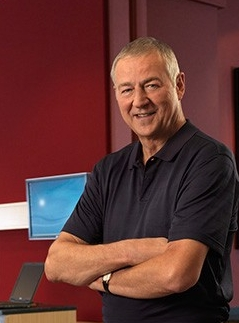
\includegraphics[width=1.4in]{goodnight}
    & 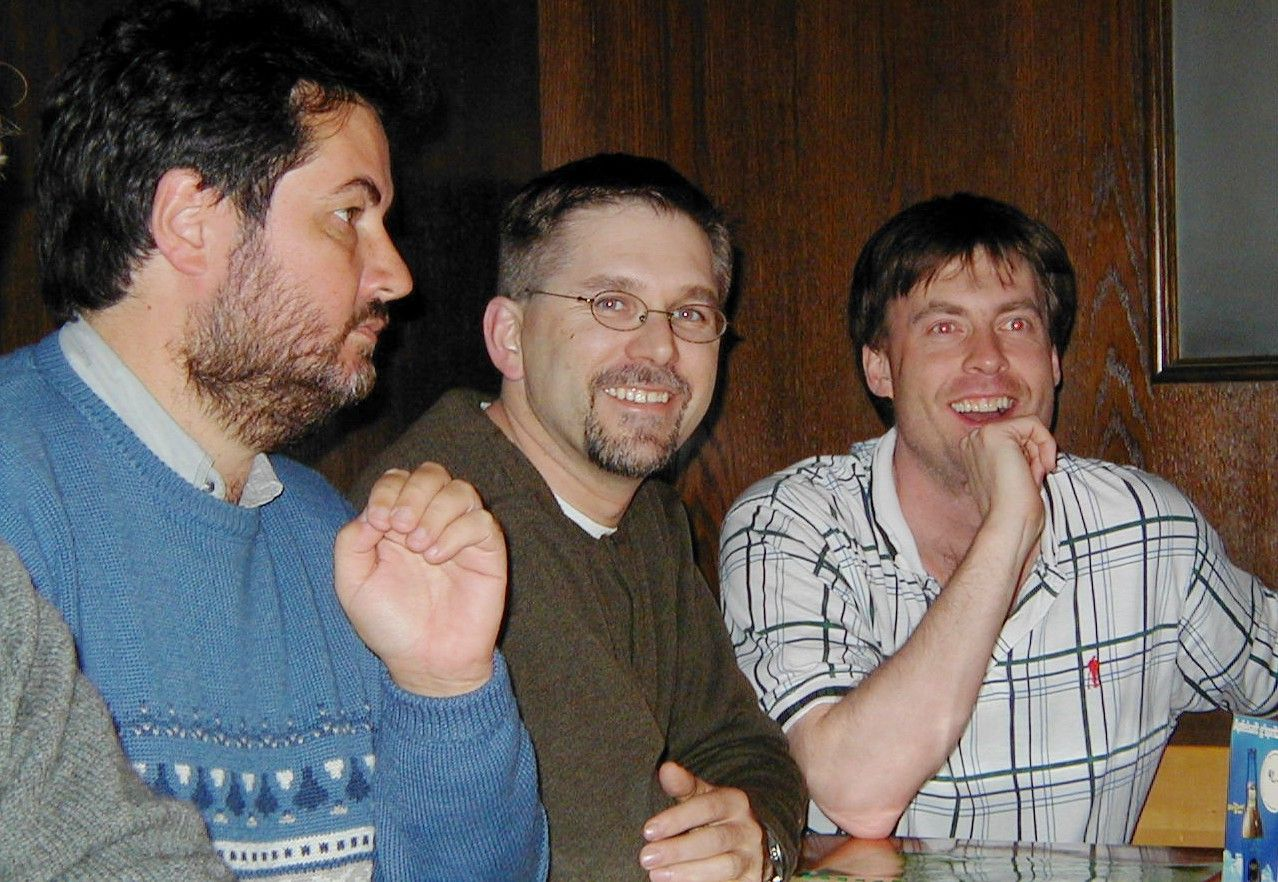
\includegraphics[width=2in]{ihaka} \\
    Jim Goodnight, CEO SAS Inc & \pbox{10cm}{Ross Ihaka\\ Robert Gentleman\\ (Duncan
    Temple Lang)\\ originators of R}
  \end{tabular}
  
\end{frame}

\begin{frame}{History}
  
  \begin{tabular}{p{0.45\textwidth}p{0.49\textwidth}}
    \textbf{SAS} & \textbf{R}\\
    From late 1960s, North Carolina State.&
From 1993, New Zealand.\\                                            
    Then: punched cards, ``submit'' job, get output later.
    Still SAS's way of operating: run list of commands, get lot
      of output.& R style: enter commands one at a time, see output/graphics
      right away.\\
                 
    Commercialized, corporate ethos.             & Open-source, free. Core group, anyone can contribute.\\
    Strength: Submitting same commands again gets \emph{exactly}
      same results. (Government, industry).& 
    Grew out of commercial software S, which appeared when
      graphics terminals new (emphasis on graphics).\\
                                             & Concept of ``function'' lets you add onto R or do
      non-standard things.\\
    Long history: well-tested.&Big user community makes sure everything works.
    
  \end{tabular}
  
  \end{frame}

\begin{frame}{Installing R}

  \begin{itemize}
  \item Free, open-source. Download and run on own computer.
  \item Two things: R itself (install first) and R Studio (front end).
    \item Go to \url{https://www.r-project.org/}:
      
      \includegraphics[width=4in]{r30}
  \end{itemize}
  
\end{frame}

\begin{frame}[fragile]{Click on Download}
  
  \begin{itemize}
  \item R is stored on numerous ``mirrors'', sites around the
    world. Choose one close to you (faster), eg.\ U of T:
    
    \includegraphics[width=4in]{r39}
  \end{itemize}
  
\end{frame}


\begin{frame}[fragile]{Click U of T}
  
  \begin{itemize}
  \item Click U of T (or other mirror), get:
    
    \includegraphics[width=4in]{r32}
    
    \item Click on your operating system, eg.\ Windows.
  \end{itemize}
  
\end{frame}

\begin{frame}[fragile]{Click on Base}

      \includegraphics[width=4in]{r33}

  \begin{itemize}
  \item Click on ``base'' here.
  \end{itemize}
  
\end{frame}


\begin{frame}[fragile]{The actual download}
  
  \begin{itemize}
  \item Click the top link below:
    
    \includegraphics[width=4in]{r34}
    
  \item Then install usual way.
  \end{itemize}
  
\end{frame}


\begin{frame}[fragile]{Now, R Studio}
  
  \begin{itemize}
  \item Go to \url{https://www.rstudio.com/}.
  \item Scroll down to this, and click Learn More (the left one):
    
    \includegraphics[width=3in]{r35}
  \end{itemize}
  
\end{frame}

\begin{frame}[fragile]{Scroll down}
  
  \begin{itemize}
  \item Scroll down to this:
    
    \includegraphics[width=4in]{r37}
    
  \item Click ``Download RStudio Desktop''.
  \end{itemize}
  
\end{frame}

\begin{frame}[fragile]{Find the one for you}
  
  \begin{itemize}
  \item Scroll down, and click the installer for your machine
    (Windows, Mac, 4 flavours of Linux). Install as usual.
    
    \includegraphics[width=4in]{r40}
  \end{itemize}
  
\end{frame}


\begin{frame}[fragile]{Running R}
  
  \begin{itemize}
  \item All of above only done \emph{once}.
  \item To run R, run \textbf{R Studio}, which itself runs R.
  \end{itemize}
  
\end{frame}

\begin{frame}[fragile]{How R Studio looks when you run it}
  
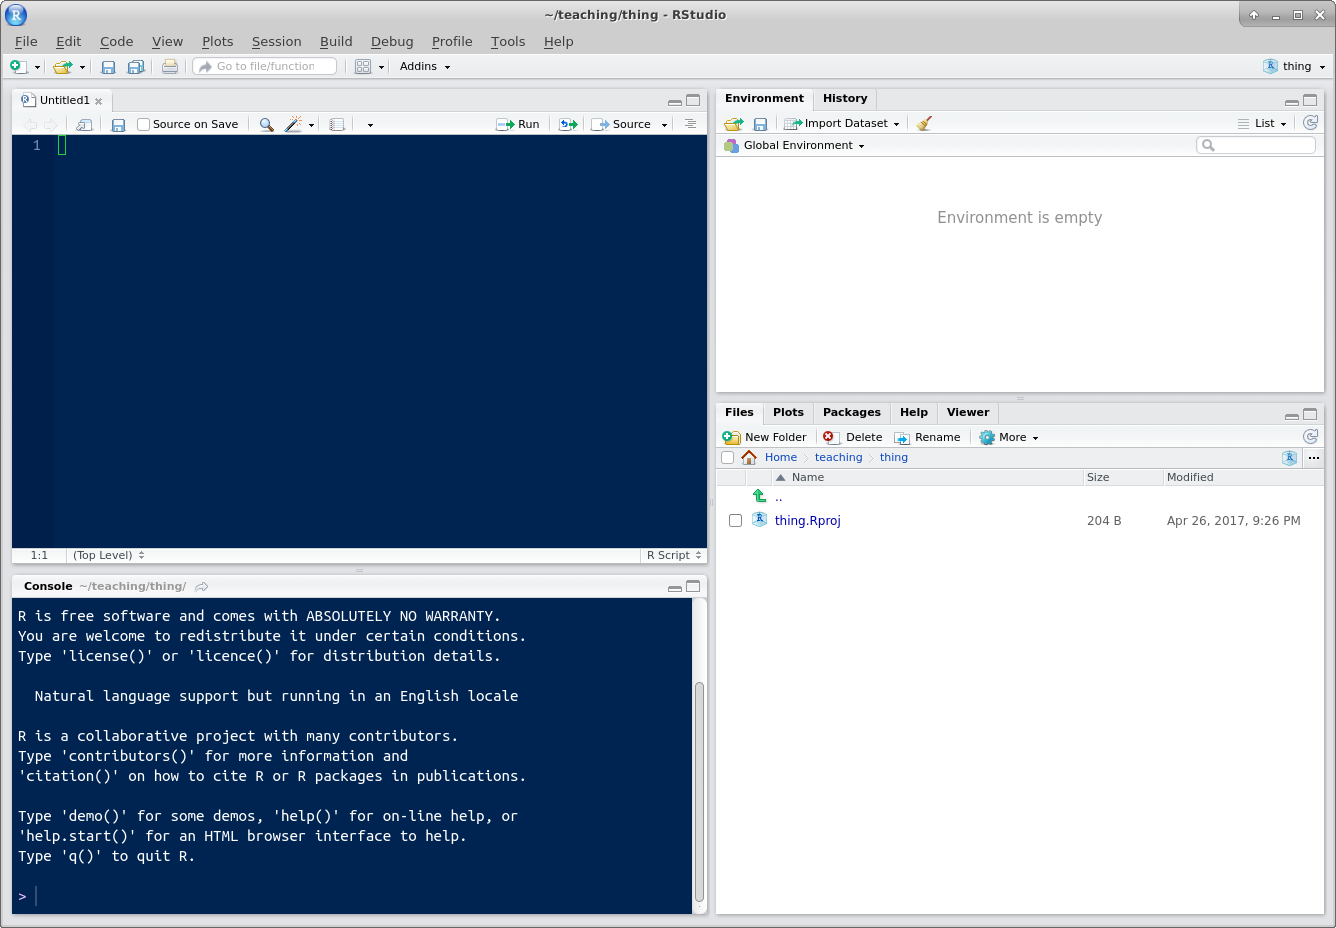
\includegraphics[width=0.8\textwidth]{rstudio-startup}
  
First time you run R Studio, click on Console window, and, next to the
\texttt{>}, type \texttt{install.packages("tidyverse")}. Let it do
what it needs to.
\end{frame}


\begin{frame}[fragile]{Connecting to SAS}

  \begin{itemize}
  \item SAS on your own computer big, expensive.
  \item U of T has ``site licence'' allows us to buy SAS for own
    computer (re-licensed every year, etc.)
  \item SAS offers ``SAS Studio'' that is free for the academic
    world. This runs through a web browser (accessible everywhere)
    with everything hosted on SAS's servers, or on a ``virtual
    machine'' on own computer.
  \item The hard part is getting registered for it.
  \end{itemize}
  
\end{frame}

\begin{frame}[fragile]{Getting registered for online version}

  \begin{itemize}
  \item Go to \url{https://odamid.oda.sas.com}. Get to this:

\includegraphics[height=0.6\textheight]{sas1}

\item Bookmark this page.
\item Go down to ``Don't have an account?'' and click ``Register Here''.
  \end{itemize}
  
\end{frame}

\begin{frame}[fragile]{Enter your name and e-mail}

\ldots and select country (Canada):

\includegraphics[width=3in]{sas2}
  
\end{frame}

\begin{frame}[fragile]{Go check your e-mail}

and look for something like this:

\includegraphics[width=3in]{sas3}

Click on the link.
  
\end{frame}

\begin{frame}[fragile]{Choose a password}

\includegraphics[height=0.7\textheight]{sas5}

  \begin{itemize}
  \item Click orange Create Account. You then get a user ID. Make a note of it.
  \item This completes the registration. You only do this once.
  \end{itemize}
  
\end{frame}

\begin{frame}[fragile]{Log into SAS}

Go back to the page you bookmarked earlier:

\includegraphics[height=0.7\textheight]{sas1b}

Type your user ID and password into the boxes, and click Sign In.
  
\end{frame}


\begin{frame}[fragile]{The dashboard}

\includegraphics[width=\textwidth]{sas6}

On the Dashboard, click SAS Studio. (Ignore the stuff about the
courses.) 
  
\end{frame}

\begin{frame}[fragile]{SAS, as you see it}

Something like this:

\includegraphics[scale=0.3]{sas-webed-opening}
  
\end{frame}


%\begin{frame}[fragile]{Trying out SAS}
%
%Go to the right side of the window, under Program 1, click on Code,
%and type the following into the window with the numbered lines:
%
%\includegraphics[scale=0.4]{prog1}
%
%When you have this to your satisfaction, click the ``running
%humanoid'' under Code. (This is called ``submitting'' in SAS jargon.)
% 
%\end{frame}
%
%\begin{frame}[fragile]{Output}
%
%If everything was correct, the Results tab under Program 1 will be
%selected, and you'll see your results, thus:
%
%\includegraphics[scale=0.35]{results1}
%
%These are: a listing of your data (from \texttt{proc print}) and a
%summary of the data, including mean and SD (from \texttt{proc means}).
%  
%\end{frame}
%
%\begin{frame}[fragile]{Errors}
%  
%  \begin{itemize}
%  \item Let me make a deliberate mistake: I left off the semicolon on the end
%of \texttt{proc print}.
%\item  When I submitted this, the Log tab popped up
%with a whole bunch of stuff including this:
%
%\includegraphics[scale=0.35]{sas-error}
%
%\item When SAS hit \texttt{proc means}, expecting a semicolon (to
%finish off the \texttt{proc print;}), but didn't see one. So error
%was \emph{just before} where the mark was. 
%
%\item Tactic: fix the \emph{first} error and submit again. (That
%first error might have caused a bunch of others.)  
%
%  \end{itemize}
%
%
%
%
%\end{frame}


\begin{frame}[fragile]{Installing SAS on your own machine}

  \begin{itemize}
  \item Pro: not dependent on SAS's servers.
  \item Con: fiendishly complicated!
  \item On your own computer, SAS runs in ``virtual machine'' (so
    doesn't matter what OS you have, as long as the virtual machine
    runs on it).
  \end{itemize}
  
\end{frame}

%%%%%%%%%%%%% 2016 version

\begin{frame}[fragile]{Getting SAS for your own machine}
  
  \begin{itemize}
  \item Go to \url{sas.com} and navigate to Products and Solutions,
    then SAS University Edition, or
    go to \url{http://www.sas.com/en_ca/software/university-edition.html}.
  \item See this:
    
    \includegraphics[width=4in]{sas16}
  \end{itemize}
  
\end{frame}

\begin{frame}[fragile]{And then}
  
  \begin{itemize}
  \item Click Get Free Software. See this:
    
    \includegraphics[width=3in]{sas28}
    
  \item Click Download Now on the \emph{left}.
  \end{itemize}
  
\end{frame}

\begin{frame}[fragile]{Select operating system}
  
  \begin{itemize}
  \item by clicking appropriate tab, eg:
    
    \includegraphics[width=4in]{sas17}
  \end{itemize}
  
\end{frame}

\begin{frame}[fragile]{Starting setup}
  
  \begin{itemize}
  \item Click tab for your operating system, and check that your
    system is good.
  \item Scroll down (4 steps):
    
    \includegraphics[width=3.5in]{sas18}
    
  \end{itemize}
  
\end{frame}

\begin{frame}[fragile]{Download VirtualBox}
  
  \begin{itemize}
  \item SAS runs on ``virtual machine'' (has own operating system
    regardless of what yours is). Download and install virtual machine:
    
    \includegraphics[width=4in]{sas19}
  \end{itemize}
  
\end{frame}


\begin{frame}[fragile]{Scroll down some more}
  
  \begin{itemize}
  \item You will be downloading a 1.7GB ``app'' (this may take a while). You may
    have to create a username/password first (next page):
    
    \includegraphics[width=2.5in]{sas20}
  \end{itemize}
  
  
\end{frame}

\begin{frame}[fragile]{Creating a ``profile''}
  
  \begin{itemize}
  \item New User on the right (unless you already have a SAS profile):

      \includegraphics[width=4in]{sas22}

  \end{itemize}
  
  
\end{frame}

\begin{frame}[fragile]{Finally, step 4}
  
  \begin{itemize}
  \item Follow the steps in the Quick Start Guide. Step 1 you probably
    already did:
    
    \includegraphics[width=4in]{sas23}
  \end{itemize}
  
\end{frame}

\begin{frame}[fragile]{Quick Start step 2}
  
  \begin{itemize}
  \item Follow the instructions. This attaches the ``app'' to your
    virtual machine so that it will run:
    
    \includegraphics[width=4in]{sas24}
  \end{itemize}
  
\end{frame}

\begin{frame}[fragile]{Step 3: setting up file access}
  
  \begin{itemize}
  \item This is kind of complicated, but follow the steps through, and
    then you can read in data files:
    
    \includegraphics[width=4in]{sas25}
  \end{itemize}
  
\end{frame}

\begin{frame}[fragile]{Start SAS}
  
  \begin{itemize}
  \item All of the above you only do once (installation).
  \item To start SAS, do the below (every time):
    
    \includegraphics[width=4in]{sas26}
  \end{itemize}
  
\end{frame}


\begin{frame}[fragile]{SAS Studio online and on your machine}

  \begin{itemize}
  \item SAS Studio runs identically whether it's online or on your machine.
  \item With one exception: accessing files (typically data files).
  \item Otherwise, any reference to SAS Studio applies equally well to
    either version.
  \end{itemize}
  
\end{frame}


\begin{frame}[fragile]{Accessing data files in SAS Studio}

    \begin{itemize}
    \item Depends on whether you're running SAS Studio online or on
      your computer.
    \item If you're running online, you have a username that you used
      for logging in, like \texttt{ken} or \texttt{megan3}.
    \item Online: access file as \texttt{/home/} plus your username
      plus filename: eg.\ \texttt{/home/megan3/mydata.txt}.
    \item On your computer: \texttt{/folders/myfolders/} plus
      filename, eg.\ \texttt{/folders/myfolders/mydata.txt}.
    \item Slashes in both cases are \emph{forward} slashes, and you
      need one to start the filename.
    \end{itemize}
    
\end{frame}

%\begin{frame}[fragile]{Using SAS Studio to save a data file}
%
%Works on either version of SAS Studio. 
%
%Create a new ``SAS Program'' (only it won't be) and
%type/copy these, as shown, into the Code window:
%
%\begin{columns}
%  
%  \begin{column}{0.3\textwidth}
%{\small
%\begin{verbatim}
%a 20
%a 21
%a 16
%b 11
%b 14
%b 17
%b 15
%c 13
%c 9
%c 12
%c 13
%\end{verbatim}
%}
%    
%  \end{column}
%
%  \begin{column}{0.65\textwidth}
%\begin{itemize}
%\item Save into file \texttt{three.txt}. Select My Folders as
%  folder to save in. SAS puts \texttt{.sas} on the
%  file name. Find the file in the Folders window, right-click, select
%  Rename, and make the filename what you really wanted.
%\end{itemize}
%    
%  \end{column}
%
%  
%\end{columns}
%
%  
%\end{frame}
%
%
%\begin{frame}[fragile]{Analysis 1(a): reading in and verifying the data}
%
%  \begin{itemize}
%\item This version if you're accessing SAS Studio online.
%\item Create a new SAS program, and enter its code thus (in the Code
%  tab):
%  
%\begin{semiverbatim}
%data groups;
%  infile '/home/ken/three.txt';
%  input group $ y;
%
%proc print;    
%\end{semiverbatim}
%  
%
%\item Replace \texttt{ken} with your online SAS Studio username.
%
%\item Code much cleaner with data in separate file.
%
%  \end{itemize}
%
%
%\end{frame}
%
%
%\begin{frame}[fragile]{Analysis 1(b): reading in and verifying the data}
%
%  \begin{itemize}
%\item This version if you're accessing SAS Studio on your own computer
%  (via virtual machine).
%\item Create a new SAS program, and enter its code thus (in the Code
%  tab):
%  
%  
%
%\begin{Datastep}
%data groups;
%  infile '/folders/myfolders/three.txt';
%  input group $ y;
%\end{Datastep}
%
%\begin{Sascode}[store=threea]
%proc print;  
%\end{Sascode}
%
%
%
%\item We'll see output in a moment. Same both ways.
%  \end{itemize}
%
%
%\end{frame}
%
%\begin{frame}[fragile]{Output}
%  
%\Listing[store=threea]{threeaa}
%
%
%\end{frame}
%
%\begin{frame}[fragile]{Folder menu}
%
%\includegraphics[width=\textwidth]{folder-menu}
%  
%\end{frame}
%
%\begin{frame}[fragile]{Code menu}
%
%\includegraphics[width=\textwidth]{code-menu}
%  
%\end{frame}
%
%
%\begin{frame}[fragile]{Results menu}
%
%\includegraphics[width=\textwidth]{results-menu}
%  
%\end{frame}
%
%
%\begin{frame}{Other notes}
%
%  \begin{itemize}
%
%  \item When saving your code, SAS appends a \texttt{.sas} to the name
%    you supply. You'll see your code file appear on the left, under Folders.
%  \item To open code, double-click on the code file
%    name under Folders. A new tab will appear with the code file.
%  \item These files all live on the SAS server or virtual machine. To make a copy of a
%    file on your own computer, click the down-arrow ``download'' button.  You'll be
%    prompted to open or save the file.
%  \item You can also upload files. Click the up-arrow ``upload''
%    button, and click Choose Files to select the file to upload. The
%    folder with a name like \texttt{/home/ken} is your file
%    storage on the SAS server, or \texttt{/folders/myfolders} on the
%    virtual machine.
%  \item You can create subfolders. Click on New SAS Program, select
%    Folder and give the new folder a name.  
%  \end{itemize}
%  
%\end{frame}
%
%
%
%\begin{frame}[fragile]{Analysis/output 2: means by group}
%
%Go back to Code tab, enter this code below what was there
%before, and submit whole thing again:
%
%
%\begin{Sascode}[store=threeb]
%proc means;
%  class group;
%  var y;    
%\end{Sascode}
%
%\Listing[store=threeb,fontsize=scriptsize]{threebb}
%
%
%\end{frame}
%
%\begin{frame}[fragile]{Analysis 3: boxplots}
%\begin{Sascode}[store=threec]
%proc sgplot;
%  vbox y / category=group;
%\end{Sascode}
%
%\Graphic[store=threec,scale=0.5]{threecc}
%
%\end{frame}
%
%\begin{frame}{Conclusions}
%
%Both boxplots and \texttt{proc means} support idea that group A has
%largest values and group C has smallest.
%  
%\end{frame}
%
%
%\begin{frame}[fragile]{Copying into SAS}
%  
%  \begin{itemize}
%  \item Copying \emph{into} SAS mostly easy: copy as normal, paste
%    into Code tab.
%  \item If copying from spreadsheet, like this,
%
%\includegraphics[width=3in]{s-data}
%
%values separated by
%    \emph{tabs}. Steps:
%    \begin{itemize}
%    \item Copy into SAS code tab as usual.
%    \item Save into file, eg.\ \texttt{x.dat}.
%    \item Read in as below (note \texttt{expandtabs}):
%    \end{itemize}
%  \end{itemize}
%
%\end{frame}
%
%\begin{frame}[fragile]{Reading a spreadsheet}
%
%\begin{Datastep}
%data x;
%  infile '/folders/myfolders/x.dat' expandtabs;
%  input a b c;  
%\end{Datastep}
%  
%\begin{Sascode}[store=xa]
%proc print;
%\end{Sascode}
%
%\Listing[store=xa]{xaa}
%
%Without \texttt{expandtabs}, get many incomprehensible error messages,
%or no data at all!
%  
%\end{frame}
%
%\begin{frame}{Copying \emph{out} of SAS}
%
%  \begin{itemize}
%    \item Results: export as \texttt{.rtf} file and open in eg.\
%      Word. Can paste several of these together into one Word doc
%      (eg.\ for assignment).
%  \item Copy and paste code from Code window. SAS code should be \texttt{fixed-pitch font}
%    (eg.\ Courier) in your document.
%  \item If all else fails, take screen shots (alt-PrintScreen), paste
%    into doc as images.
%  \end{itemize}
%  
%\end{frame}
%
%\begin{frame}[fragile]{Using R}
%
%  \begin{itemize}
%  \item Mimic above ``analysis'' using R.
%  \item Run commands one at a time, see results right away.
%  \item See \emph{errors} right away too!
%  \item Start up R Studio, go to Console window (bottom left). See
%    \texttt{>} prompt: waiting for you. Try:
%
%<<>>=
%  x=c(1,2,3,5,7)
%@     
%    
%\item ``Glue values together into list, and call it \texttt{x}''.
%\item No comment equals no error.
%\pause
%\item Display anything in R by entering its name:
%
%<<>>=
%x
%@   
%
%\item showing that \texttt{x} really does contain those values.
%
%
%  \end{itemize}
%  
%\end{frame}
%
%\begin{frame}[fragile]{Basic statistics}
%
%  \begin{itemize}
%  \item Mean:
%
%<<>>=
%mean(x)
%@     
%\pause
%  \item SD:
%
%<<>>=
%sd(x)
%@     
%\pause
%\item Quartiles also by function \texttt{summary}:
%
%<<>>=
%summary(x)    
%@   
%
%\item Five-number summary plus mean. For percentiles use
%  \texttt{quantile}, eg.\ 60th percentile:
%
%<<>>=
%quantile(x,0.60)  
%@   
%
%\item Errors come out in red immediately. Output (results) in black.
%\item Command history: up and down arrows take you to all the commands
%  you entered.
%
%  \end{itemize}
%  
%\end{frame}

%\begin{frame}{Projects and R scripts}
%
%  **** this may need moving ****
%  
%  \begin{itemize}
%  \item Can use R from Console window, copy commands and output into Word.
%  \item But better organization by using a Project and R script.
%  \item \textbf{Project}: container for commands, data, stuff associated with
%    one piece of work:
%    \begin{itemize}
%    \item Project-Create Project.
%    \item Use current folder for project or create new one. 
%    \item ``Browse''
%      to navigate to folder.
%    \item R Studio switches to new project.
%    \end{itemize}
%    \pause
%  \item \textbf{Script}: like string of commands fed into SAS, but more flexible.
%    \begin{itemize}
%    \item File-New-R Script. Creates top left window for commands to
%      use (and re-use).
%    \item File-Save as usual. No file extension needed (R Studio
%      supplies one.)
%    \end{itemize}
%  \end{itemize}
%  
%\end{frame}
%
%\begin{frame}[fragile]{Running a script}
%  
%  \begin{itemize}
%    \item To run:
%      \begin{itemize}
%      \item ``Source'' runs everything.
%      \item ``Run'' (or Control/Cmd-Enter) runs code on current line.
%      \item Select several lines: Run or Control-Enter runs selected lines.
%      \end{itemize}
%      \pause
%    \item Commands and output appear in Console window; copy-paste to
%      a report. 
%    \item Save a script to be able to rerun any commands later. (Don't
%      have to remember what you did.)
%  \end{itemize}
%  
%\end{frame}
%
%\begin{frame}[fragile]{Reading data from a file}
%  \begin{itemize}
%  \item ``basic'' way: one observation per line, values for all variables
%separated by whitespace. (Like SAS.)
%
%\item The top-left of R-studio also text editor. 
%\item Create new data file with File, New, Text File 
%\item Open existing data file, eg.\ \texttt{threegroups.txt} as
%we used with SAS. (This file has different name because it has a row
%of headers.)
%\item With R, put the variable names on the first line of the data
%file, like this. Saved as \texttt{threegroups.txt}:
%
%\begin{verbatim}
%group y
%a 20
%a 21
%a 16
%b 11
%...
%\end{verbatim}
%  \end{itemize}
%
%\end{frame}
%
%\begin{frame}[fragile]{Reading data in}
%
%  \begin{itemize}
%  \item Tell R that first row is headers:
%
%<<>>=
%  mydata=read.table("threegroups.txt",header=T)
%  mydata  
%@     
%
%
%  \end{itemize}
%  
%\end{frame}
%
%\begin{frame}[fragile]{Reading data in (2)}
%  
%  \begin{itemize}
%  \item If no headers, say \texttt{header=F}, R supplies column names:
%    
%<<>>=
%  mydata2=read.table("threegroups.dat",header=F)
%  mydata2 
%@     
%  \end{itemize}
%  
%\end{frame}
%
%\begin{frame}[fragile]{Data frames}
%
%  \begin{itemize}
%  \item \texttt{mydata} holding data values called
%\textbf{data frame}: rectangular array with rows and columns,
%rows observations (individuals) and columns
%variables.
%\item Access variable like this:
%
%<<>>=
%  mydata$y
%@   
%
%%$ %$ %$
%\item Or like this:
%<<>>=
%  attach(mydata)
%  y
%@ 
%\item Logic: no variable \texttt{y}, but if \texttt{attach} a
%data frame, variables looked for there as well. Here, \texttt{y} must
%be \texttt{mydata\$y}, since there is no other \texttt{y}.
%
%  \end{itemize}
%  
%\end{frame}
%
%\begin{frame}[fragile]{Polluting the name space}
%  
%  \begin{itemize}
%\item Problem with \texttt{attach}: many extra
%variables; ``where did
%that \texttt{y} and \texttt{group} come from
%anyway?'' (``polluting the name space''.)
%\item If was \emph{already} a \texttt{y} defined, which one do you
%  see? Not clear.
%\item When finished with \texttt{attach}ed
%variables: \texttt{detach(mydata)},
%now no ``extra'' \texttt{y} or
%\texttt{group} any more.
%  \end{itemize}
%  
%\end{frame}
%
%\begin{frame}[fragile]{Means by group}
%
%  \begin{itemize}
%  \item Not quite as easy as SAS, but more flexible:
%
%<<>>=
%  aggregate(y~group,mydata,mean)
%@     
%
%\item This works whether or not you \texttt{attach}ed the data frame.
%\item Three things:
%  \begin{itemize}
%  \item ``Model formula'': variable calculating for, squiggle,
%    grouping variable.
%  \item Data frame containing those variables.
%  \item Thing to calculate.
%  \end{itemize}
%\end{itemize}
%
%\end{frame}
%
%\begin{frame}[fragile]{Other things by group}
%
%  \begin{itemize}
%\item IQR by group like this:
%<<>>=
%aggregate(y~group,data=mydata,IQR)  
%@   
%\item Feed in calculation variable, grouping variable, data frame,
%  thing to calculate.
%\item See model formula again in a few seconds when we draw a boxplot.
%  \end{itemize}
%  
%\end{frame}
%
%\begin{frame}[fragile]{Boxplot}
%
%<<fig.height=4>>=
%  boxplot(y~group,data=mydata)
%@ 
%
%\end{frame}
%
%\begin{frame}[fragile]{Comments}
%
%\begin{itemize}
%
%\item ``Silly'' boxplots with not much data.
%\item Different from SAS because different quartile definition.
%\item In R Studio, plot appears bottom right.
%\item Can omit grouping variable to get boxplot of all values.
%
%\end{itemize}
%  
%\end{frame}
%
%\begin{frame}[fragile]{Another boxplot}
%
%To get boxplot of \emph{all} values in \texttt{y}, not subdivided by
%group, do this:
%
%<<fig.height=3.5>>=
%boxplot(mydata$y)
%@ 
%%$
%
%We see how to get better boxplots as part of \texttt{ggplot} later.
%
%%$ %$
%
%
%\end{frame}
%
%\begin{frame}{Multiple graphs in R Studio}
%
%  \begin{itemize}
%  \item If you made the last two boxplots in R Studio, second one came
%    up on top of first one.
%  \item Use arrows below Plots tab to cycle among your graphs.
%  \item Limit of 30 graphs saved.
%  \end{itemize}
%  
%\end{frame}
%
%\begin{frame}[fragile]{Reading data from a spreadsheet}
%
%  \begin{itemize}
%  \item Best way, for R: save data as \texttt{.csv} file (File, Save As)
%  \item \texttt{.csv} saves values, not formulas.
%  \item Example:
%
%  \includegraphics[width=0.4\textwidth]{small}
%\item Columns have no names.
%\item Save as \texttt{small.csv} in project folder.
%  \end{itemize}
%  
%\end{frame}
%
%\begin{frame}[fragile]{Reading into R}
%
%  \begin{columns}
%    \begin{column}{0.6\textwidth}
%
%<<>>=
%zz=read.csv("small.csv",header=F)
%zz   
%@       
%
%<<>>=
%mynames=c("Foo","Blah","Ding")
%names(zz)=mynames
%zz 
%@ 
%
%      
%    \end{column}
%    \begin{column}{0.4\textwidth}
%      \begin{itemize}
%      \item No column names; R supplied some. Can change.
%        \bigskip
%        \bigskip
%        \bigskip
%      \item Data frame now has supplied names.
%      \end{itemize}
%
%      
%    \end{column}
%  \end{columns}
%
%
%\end{frame}
%
%\begin{frame}[fragile]{Reading \texttt{.csv} files into SAS}
%
%\texttt{dlm} short for ``delimiter'':
%
%\begin{Datastep}
%data stuff;
%  infile '/folders/myfolders/small.csv' dlm=',';
%  input foo blah ding;  
%\end{Datastep}
%
%\begin{Sascode}[store=ia]
%proc print;
%\end{Sascode}
%
%\Listing[store=ia]{iaa}
%  
%\end{frame}
%
%\begin{frame}[fragile]{Alternatively in R}
%
%via copy and paste:
%
%\begin{itemize}
%\item Open new Text File in R Studio.
%\item Paste spreadsheet values into empty window.
%\item Save as eg.\ \texttt{small.txt}.
%\item Into R via \texttt{read.table}
%\end{itemize}
%
%<<>>=
% fred=read.table("small.txt",header=F)
% fred
%@ 
%
%Don't know whether pasting introduced tabs, but R handled it OK.
%  
%\end{frame}
%
%\begin{frame}[fragile]{\texttt{read.table} vs.\ \texttt{read.csv}}
%
%  \begin{itemize}
%  \item \texttt{read.csv} simplified version of \texttt{read.table},
%    especially for reading \texttt{.csv} files. These are same:
%
%<<>>=
%fred1=read.csv("small.txt",header=F)
%fred2=read.table("small.txt",sep=",",header=F)  
%@     
%
%  \end{itemize}
%  
%\end{frame}
%
%\begin{frame}[fragile]{``Compiling a notebook'' 1/4}
%  
%  \begin{itemize}
%  \item   This is the way to handle R code for handing in work.
%  \item Alternative (later) is R Markdown.
%  \item Imagine you have an assignment question like this:
%    \begin{enumerate}
%    \item The variable $x$ has data values 10,11,13,15,16,17,19,24,32.
%      \begin{enumerate}
%      \item[(a)] Read the data into R and demonstrate that you read in the
%        correct values.
%      \item[(b)] Obtain the mean and median of $x$. Does the distribution
%        appear to be skewed or symmetric? Explain briefly.
%      \item[(c)] Obtain a boxplot of $x$. Does the boxplot support your
%        conclusion from the previous part? Explain briefly.
%      \end{enumerate}
%    \end{enumerate}
%  \item Create a script window that contains the code to produce
%    output you want. (You may not get this right the first time;
%    persevere until you do.) Save the script.
%
%  \end{itemize}
%  
%\end{frame}
%
%\begin{frame}[fragile]{``Compiling a notebook'' 2/4}
%
%  
%  \begin{itemize}
%  \item   My script, called \texttt{xcode.R}:
%  
%  \includegraphics[width=0.7\textwidth]{W093}
%  
%  
%\item To your script, add ``comment lines'' that actually answer the
%  questions asked (in general, that explain what the output
%  means). 
%\item The ``comment lines'' begin with the symbols \texttt{\#'}
%  (shift-3 and single-quote). If you press Enter, you'll get the
%  comment characters ready for another line. If you don't want them,
%  delete them.
%\item A comment line with no text will start a new line in the output.
%
%  \end{itemize}
%  
%\end{frame}
%
%\begin{frame}[fragile]{``Compiling a notebook'' 3/4}
%  
%  \begin{itemize}
%  \item   This is mine, with text attached:
%  
%  \includegraphics[width=0.8\textwidth]{W094}
%
%  
%\item Note the empty lines \emph{before} each part of the answer.
%\item Find ``Source on Save'' at the top, go right to thing that looks
%  like paper notebook, click:
%  \end{itemize}
%  
%  
%\end{frame}
%
%\begin{frame}[fragile]{``Compiling a notebook'' 4/4}
%  
%  \begin{itemize}
%    \item \ldots and change Output Format to MS Word:
%
%      \includegraphics[width=0.5\textwidth]{W095}
%      
%      
%    \item Click Compile. You'll see a Word document with the code,
%      output and comments in it, in the right format to form part of
%      an assignment.
%    \item For assignment, copy-and-paste into one document all the
%      \texttt{.rtf} documents that came out of SAS and all the
%      compiled notebooks that came out of R Studio.
%  \end{itemize}
%  
%  
%\end{frame}




% reading in datafiles


\section{Reading data from files}

\frame{\sectionpage}

\begin{frame}[fragile]{Introduction}
  
  \begin{itemize}
  \item First thing we need to do is to read in data, so that we can
    use our software to analyze.
  \item Both R and SAS.
  \item Consider these:
    \begin{itemize}
    \item Spreadsheet data saved as \texttt{.csv} file.
    \item ``Delimited'' data such as values separated by spaces.
    \item Actual Excel spreadsheets.
    \end{itemize}
  \end{itemize}
  
\end{frame}

\begin{frame}[fragile]{A spreadsheet}
  
  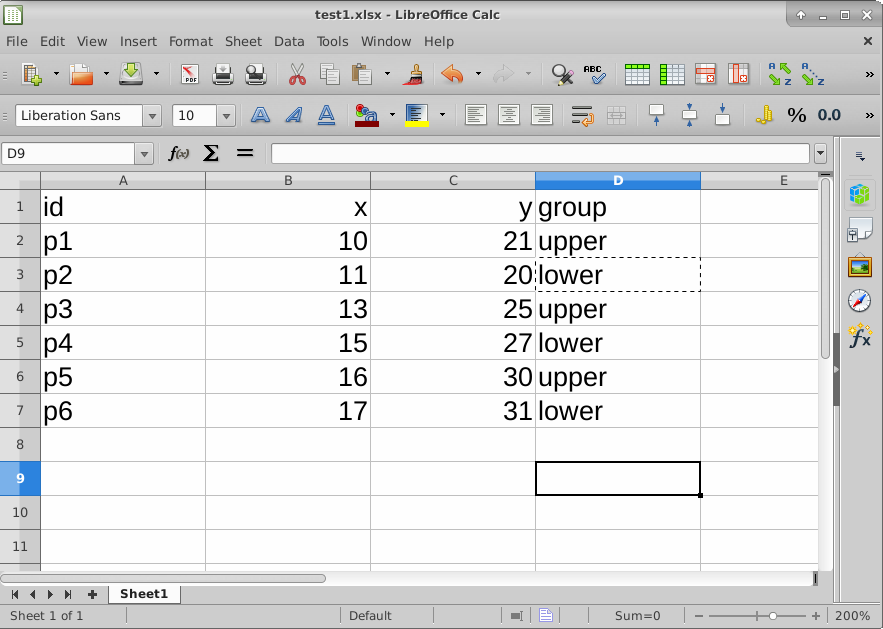
\includegraphics[width=0.9\textwidth]{spreadsheet}
  
\end{frame}

\begin{frame}[fragile]{Save as \texttt{.csv}}
  
  \begin{itemize}
  \item \texttt{.csv} or ``comma-separated values'' is a way of
    turning spreadsheet values into plain text.
  \item Easy to read into R or SAS
  \item but does \emph{not} preserve formulas. (This is a reason for
    doing \emph{all} your calculations in your statistical software,
    and \emph{only} having data in your spreadsheet.)
  \item File, Save As Text CSV (or similar).
  \end{itemize}
  
\end{frame}

\begin{frame}[fragile]{The \texttt{.csv} file}
  
\verbatiminput{test1.csv}
  
\end{frame}


\begin{frame}[fragile]{Reading file in R}
  
  
  \begin{itemize}
  \item Start (as always) with

\begin{knitrout}\footnotesize
\definecolor{shadecolor}{rgb}{0.969, 0.969, 0.969}\color{fgcolor}\begin{kframe}
\begin{alltt}
\hlkwd{library}\hlstd{(tidyverse)}
\end{alltt}


{\ttfamily\noindent\itshape\color{messagecolor}{\#\# Loading tidyverse: ggplot2\\\#\# Loading tidyverse: tibble\\\#\# Loading tidyverse: tidyr\\\#\# Loading tidyverse: readr\\\#\# Loading tidyverse: purrr\\\#\# Loading tidyverse: dplyr}}

{\ttfamily\noindent\itshape\color{messagecolor}{\#\# Conflicts with tidy packages ----------------------------------------------}}

{\ttfamily\noindent\itshape\color{messagecolor}{\#\# filter(): dplyr, stats\\\#\# lag():\ \ \ \ dplyr, stats}}\end{kframe}
\end{knitrout}

If you don't get this, do this (should only need it once):

\begin{knitrout}
\definecolor{shadecolor}{rgb}{0.969, 0.969, 0.969}\color{fgcolor}\begin{kframe}
\begin{alltt}
\hlkwd{install.packages}\hlstd{(}\hlstr{"tidyverse"}\hlstd{)}
\end{alltt}
\end{kframe}
\end{knitrout}



  \end{itemize}
  
\end{frame}

\begin{frame}[fragile]{Finding the file}
  \begin{itemize}
\item Run this:
 

\begin{knitrout}
\definecolor{shadecolor}{rgb}{0.969, 0.969, 0.969}\color{fgcolor}\begin{kframe}
\begin{alltt}
\hlstd{f}\hlkwb{=}\hlkwd{file.choose}\hlstd{()}
\end{alltt}
\end{kframe}
\end{knitrout}

This brings up a file selector. Use it to find your \texttt{.csv}
file. Then type the name \texttt{f} to display what it contains:

\begin{knitrout}
\definecolor{shadecolor}{rgb}{0.969, 0.969, 0.969}\color{fgcolor}\begin{kframe}
\begin{alltt}
\hlstd{f}
\end{alltt}
\begin{verbatim}
## [1] "/home/ken/teaching/c32/notes/2017/test1.csv"
\end{verbatim}
\end{kframe}
\end{knitrout}

(This is Linux. Mac looks similar, Windows different.)

\item Now R knows where our file is, and we can read it in (over).
  \end{itemize}
\end{frame}

\begin{frame}[fragile]{Reading in the file}
  
  \begin{itemize}
  \item Use \texttt{read\_csv} with the name of the file. Save the
    read-in file in something, here called \texttt{mydata}: 
    
\begin{knitrout}
\definecolor{shadecolor}{rgb}{0.969, 0.969, 0.969}\color{fgcolor}\begin{kframe}
\begin{alltt}
\hlstd{mydata}\hlkwb{=}\hlkwd{read_csv}\hlstd{(f)}
\end{alltt}


{\ttfamily\noindent\itshape\color{messagecolor}{\#\# Parsed with column specification:\\\#\# cols(\\\#\#\ \  id = col\_character(),\\\#\#\ \  x = col\_integer(),\\\#\#\ \  y = col\_integer(),\\\#\#\ \  group = col\_character()\\\#\# )}}\end{kframe}
\end{knitrout}
\item \texttt{read\_csv} guesses what kind of thing is in each
  column. Here it correctly guesses that:
  
  \begin{itemize}
  \item   \texttt{id} and
  \texttt{group} are text (categorical variables). \texttt{id} is
  actually ``identifier variable'': identifies
  individuals. 
\item \texttt{x} and \texttt{y} are integers (quantitative variables
  that here have no decimal point). Decimal numbers would be labelled
  \texttt{num} or \texttt{double}. 

  \end{itemize}
  

  \end{itemize}
  
\end{frame}

\begin{frame}[fragile]{Looking at what we read in}
  
  \begin{itemize}
\item Again, type the name of the thing to display it:
  
\begin{knitrout}
\definecolor{shadecolor}{rgb}{0.969, 0.969, 0.969}\color{fgcolor}\begin{kframe}
\begin{alltt}
\hlstd{mydata}
\end{alltt}
\begin{verbatim}
## # A tibble: 6 x 4
##      id     x     y group
##   <chr> <int> <int> <chr>
## 1    p1    10    21 upper
## 2    p2    11    20 lower
## 3    p3    13    25 upper
## 4    p4    15    27 lower
## 5    p5    16    30 upper
## 6    p6    17    31 lower
\end{verbatim}
\end{kframe}
\end{knitrout}

\item This is a ``tibble'' or data frame, the standard way of storing
  a data set in R.
\item Tibbles print as much as will display on the screen. If there
  are more rows or columns, it will say so.
  \end{itemize}
  
\end{frame}

\begin{frame}[fragile]{\texttt{View}-ing your data frame}
    
    \begin{itemize}
    \item Another way to examine your data frame is to View it, like this:
      
\begin{knitrout}
\definecolor{shadecolor}{rgb}{0.969, 0.969, 0.969}\color{fgcolor}\begin{kframe}
\begin{alltt}
\hlkwd{View}\hlstd{(mydata)}
\end{alltt}
\end{kframe}
\end{knitrout}

\item This pops up a ``data frame viewer'' top left:
  
  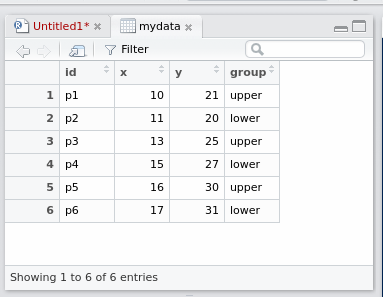
\includegraphics[width=0.6\textwidth]{viewview}
    \end{itemize}
  
\end{frame}

\begin{frame}[fragile]{What you can and cannot do with this View}
  
  \begin{itemize}
  \item Read-only: cannot edit data
  \item Can display data satisfying conditions: click on Filter, then:
    \begin{itemize}
    \item for a categorical variable, type name of category you want
    \item for a quantitative variable, use slider to describe values
      you want.
    \end{itemize}
  \item Can sort a column into ascending or descending order (click
    little arrows next to column name).
    
  \item Clicking the symbol left of Filter ``pops out'' View into
    separate (bigger) window.
  \item Cannot include in output to hand in (except by taking
    screenshot and handing \emph{that} in).
  \end{itemize}
  
\end{frame}

\begin{frame}[fragile]{Summarizing what we read in}
  
  \begin{itemize}
  \item It is \emph{always} a good idea to look at your data after you
    have read it in, to make sure you have believable numbers (and the
    right number of individuals and variables). 
  \item Sometimes the data set is too big, and you want to summarize it:
    
\begin{knitrout}
\definecolor{shadecolor}{rgb}{0.969, 0.969, 0.969}\color{fgcolor}\begin{kframe}
\begin{alltt}
\hlkwd{glimpse}\hlstd{(mydata)}
\end{alltt}
\begin{verbatim}
## Observations: 6
## Variables: 4
## $ id    <chr> "p1", "p2", "p3", "p4", "p5", "p6"
## $ x     <int> 10, 11, 13, 15, 16, 17
## $ y     <int> 21, 20, 25, 27, 30, 31
## $ group <chr> "upper", "lower", "upper", "lower", "upper", "lower"
\end{verbatim}
\end{kframe}
\end{knitrout}

\item This tells you how many observations and variables, and shows
  you the first few values (almost all of them here).
  \end{itemize}
  
\end{frame}

\begin{frame}[fragile]{Five-number summary}
  
  \begin{itemize}
  \item this way:
    
\begin{knitrout}\footnotesize
\definecolor{shadecolor}{rgb}{0.969, 0.969, 0.969}\color{fgcolor}\begin{kframe}
\begin{alltt}
\hlkwd{summary}\hlstd{(mydata)}
\end{alltt}
\begin{verbatim}
##       id                  x               y            group          
##  Length:6           Min.   :10.00   Min.   :20.00   Length:6          
##  Class :character   1st Qu.:11.50   1st Qu.:22.00   Class :character  
##  Mode  :character   Median :14.00   Median :26.00   Mode  :character  
##                     Mean   :13.67   Mean   :25.67                     
##                     3rd Qu.:15.75   3rd Qu.:29.25                     
##                     Max.   :17.00   Max.   :31.00
\end{verbatim}
\end{kframe}
\end{knitrout}

\item For quantitative variables, a five-number summary plus the mean.
\item For categorical variables, count of how many rows.
\item Quick check for errors: these often show up as values too high
  or too low, so the min and/or max will be unreasonable.
  \end{itemize}
  
\end{frame}

\begin{frame}[fragile]{Reading from a URL}
  
  \begin{itemize}
  \item Any data file on the Web can be read directly.
  \item Example data:
    \url{http://www.utsc.utoronto.ca/~butler/c32/global.csv}.
  \item Use URL instead of filename:
    
\begin{knitrout}
\definecolor{shadecolor}{rgb}{0.969, 0.969, 0.969}\color{fgcolor}\begin{kframe}
\begin{alltt}
\hlstd{url}\hlkwb{=}\hlstr{"http://www.utsc.utoronto.ca/~butler/c32/global.csv"}
\hlstd{global}\hlkwb{=}\hlkwd{read_csv}\hlstd{(url)}
\end{alltt}


{\ttfamily\noindent\itshape\color{messagecolor}{\#\# Parsed with column specification:\\\#\# cols(\\\#\#\ \  warehouse = col\_character(),\\\#\#\ \  size = col\_integer(),\\\#\#\ \  cost = col\_double()\\\#\# )}}\end{kframe}
\end{knitrout}
  \end{itemize}
  
\end{frame}

\begin{frame}[fragile]{The data}
  
\begin{knitrout}
\definecolor{shadecolor}{rgb}{0.969, 0.969, 0.969}\color{fgcolor}\begin{kframe}
\begin{alltt}
\hlstd{global}
\end{alltt}
\begin{verbatim}
## # A tibble: 10 x 3
##    warehouse  size  cost
##        <chr> <int> <dbl>
##  1         A   225 11.95
##  2         B   350 14.13
##  3         A   150  8.93
##  4         A   200 10.98
##  5         A   175 10.03
##  6         A   180 10.13
##  7         B   325 13.75
##  8         B   290 13.30
##  9         B   400 15.00
## 10         A   125  7.97
\end{verbatim}
\end{kframe}
\end{knitrout}
  
\end{frame}

\begin{frame}[fragile]{Now, in SAS}
  
  \begin{itemize}
  \item Now, do whole thing again in SAS.
  \item In SAS Studio, click on Files (Home) and find the Upload
    button (4th one in top row) (should be not greyed out):
    

\includegraphics[width=0.5\textwidth]{upload}

  \end{itemize}
  
\end{frame}

\begin{frame}[fragile]{\ldots Continued}
  
  \begin{itemize}
\item Click the Upload button, and then Choose Files in the box that
  pops up. This brings up a file selector as \texttt{file.choose} does
  in R. Find your \texttt{.csv} file, and click to ``open'' it. It
  should appear on your Upload Files box:
  
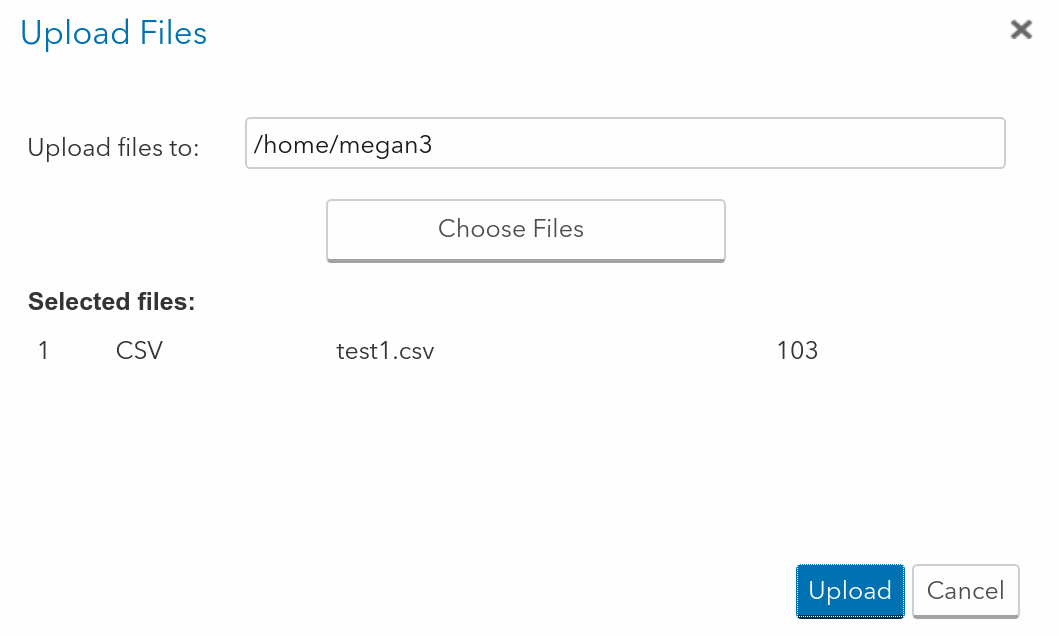
\includegraphics[width=0.5\textwidth]{upload-file}

\item Click Upload. When it's done, you should see your \texttt{.csv}
  file under Files (Home) on the left.
  \end{itemize}
  
\end{frame}

\begin{frame}[fragile]{Reading in the data}
  
  \begin{itemize}
  \item In SAS Studio, click New (leftmost button under Server Files
    and Folders) and select New SAS Program.
  \item On the right, in the Code tab, type code like this, only
    instead of \texttt{ken} put your username:
    
    \begin{Datastep}
proc import 
  datafile='/home/ken/test1.csv'
  dbms=csv
  out=mydata
  replace;
  getnames=yes;
    \end{Datastep}
    
    \begin{Sascode}[store=ra]
proc print;
    \end{Sascode}
  \item Make sure you get \emph{all} the semicolons in the right
    places!
  \item This will read in the data that you uploaded, and list the
    whole data set.
  \end{itemize}
  
\end{frame}


\begin{frame}[fragile]{Running the code}
  
  \begin{itemize}
  \item Find the ``running human'' under the word Code. Click it. 
  \item If all goes well, you should see the data set displayed in a
    Results tab:
    
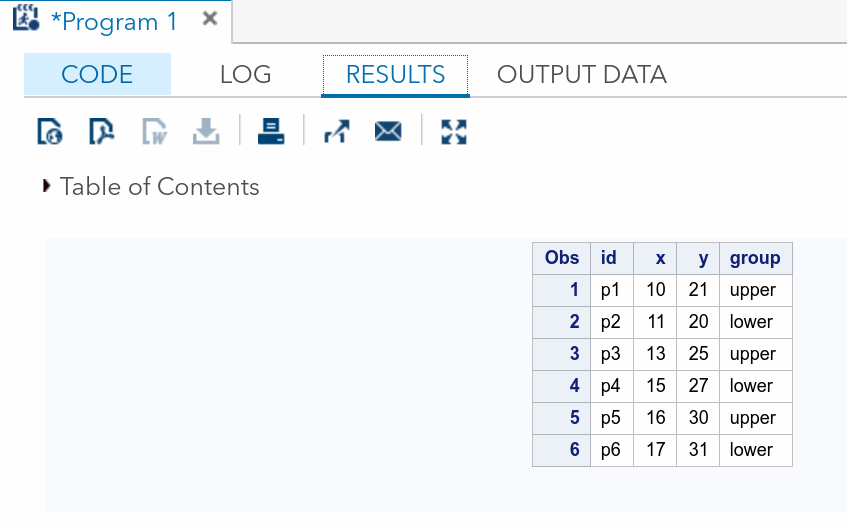
\includegraphics[width=0.7\textwidth]{sasstudio-results}

\item If not, you'll get taken to the Log tab, which will show you
  where your error was. Fix it, and try again. (SAS can sometimes
  guess what you meant, even if it's not what you typed.)
  \end{itemize}
  
\end{frame}

\begin{frame}[fragile]{That code}
  
  \begin{itemize}
  \item \texttt{proc print} displays the whole data set.
  \item The \texttt{proc import} organizes reading in the data:
    \begin{itemize}
    \item \texttt{datafile} says where to find the data file (on SAS
      Studio's server, where you uploaded it to).
    \item \texttt{dbms} says what kind of file it is, a \texttt{.csv}
      in this case.
    \item \texttt{out} gives the data set a name within SAS (that can
      be used to refer to this data set later)
    \item \texttt{getnames} means to take the variable names from the
      top line of the data file (which is usually where they are). 
    \end{itemize}
  \end{itemize}
  
\end{frame}

\begin{frame}[fragile]{Alternatively}
  
  \begin{itemize}
  \item Click the New button, but then Import Data.
  \item Find your data file on the left, and drag it across to Select
    File on the right.
  \item Some code will appear. This is (basically) the \texttt{proc
      import} code we used above.
  \item Copy the text from \texttt{FILENAME} down to \texttt{RUN;}
    (inclusive).
  \item Open a New SAS Code window. Paste the copied code into it.
  \item Add anything else at the bottom, like a \texttt{proc print},
    and run as before.
  \end{itemize}
  
\end{frame}

\begin{frame}[fragile]{Summarizing a data set}
  
  \begin{itemize}
  \item Replace the \texttt{proc print} with \texttt{proc means}:
    
    \begin{Sascode}[store=rb]
proc means;      
    \end{Sascode}
    
    That gives the mean, SD, min, max and \#observations for each
    variable (below).
    
    \item Note that you only get means for quantitative variables.
    \item \texttt{proc print}, \texttt{proc means} etc.\ work on
      \emph{the most recently created data set} (usually what you
      want). 
    
\Listing[store=rb,fontsize=scriptsize]{rbb}    


  \end{itemize}
  
\end{frame}

\begin{frame}[fragile]{Reading from a URL}
  
  \begin{itemize}
  \item A little extra setup:
    
    \begin{Sascode}[store=ua]
filename myurl 
  url "http://www.utsc.utoronto.ca/~butler/c32/global.csv";

proc import 
  datafile=myurl 
  dbms=csv
  out=global
  replace;
  getnames=yes;
  
proc print;
    \end{Sascode}
    
    
  \item The \texttt{filename} line says that the piece of text is
    actually a URL rather than a filename on this computer.
  \end{itemize}
  
\end{frame}

\begin{frame}[fragile]{Did it work?}
  
\Listing[store=ua,fontsize=footnotesize]{uaa}  
  
\end{frame}

\begin{frame}[fragile]{Space-delimited files}
  
  \begin{itemize}
  \item Another common format for data is a text file with the values
    separated by spaces. Data below in two long columns with right
    side below left side:
    
    \begin{footnotesize}
    \begin{multicols}{2}
\verbatiminput{/home/ken/coffee.txt}      
    \end{multicols}
      
    \end{footnotesize}
    
  \end{itemize}
  
\end{frame}

\begin{frame}[fragile]{Reading in these data}
  
  \begin{itemize}
  \item Change the \texttt{proc import}:
    
    \begin{Datastep}
proc import 
  datafile='/home/ken/coffee.txt'
  dbms=dlm
  out=coffee
  replace;
  delimiter=' ';
  getnames=yes;
    \end{Datastep}
  \item On \texttt{dbms}, \texttt{dlm} means ``delimited file'', that
    is, ``values separated by something''. So we have to say what the
    values are separated by, namely exactly one space. (The values
    could be separated by anything.)
  \end{itemize}
  
\end{frame}

\begin{frame}[fragile]{Did it work?}
  
  \begin{itemize}
  \item The first 15 (of 32) lines. It seems to have worked:
    
    \begin{Sascode}[store=rc]
proc print data=coffee(obs=15);      
    \end{Sascode}
    
    \Listing[store=rc,fontsize=footnotesize]{rcc}
  \end{itemize}
  
\end{frame}

\begin{frame}[fragile]{Reading the coffee data into R}
  
  \begin{itemize}
  \item Save the text file somewhere and then find it:

\begin{knitrout}
\definecolor{shadecolor}{rgb}{0.969, 0.969, 0.969}\color{fgcolor}\begin{kframe}
\begin{alltt}
\hlstd{f}\hlkwb{=}\hlkwd{file.choose}\hlstd{()}
\end{alltt}
\end{kframe}
\end{knitrout}
\begin{knitrout}
\definecolor{shadecolor}{rgb}{0.969, 0.969, 0.969}\color{fgcolor}\begin{kframe}
\begin{alltt}
\hlstd{f}
\end{alltt}
\begin{verbatim}
## [1] "/home/ken/teaching/c32/notes/2017/coffee.txt"
\end{verbatim}
\end{kframe}
\end{knitrout}
\item This time, \texttt{read\_delim}, and again we have to say what
  the thing is separating the values:
  
\begin{knitrout}
\definecolor{shadecolor}{rgb}{0.969, 0.969, 0.969}\color{fgcolor}\begin{kframe}
\begin{alltt}
\hlstd{coffee}\hlkwb{=}\hlkwd{read_delim}\hlstd{(f,}\hlstr{" "}\hlstd{)}
\end{alltt}


{\ttfamily\noindent\itshape\color{messagecolor}{\#\# Parsed with column specification:\\\#\# cols(\\\#\#\ \  cup = col\_character(),\\\#\#\ \  tempdiff = col\_double()\\\#\# )}}\end{kframe}
\end{knitrout}

\item Name of the cup, text, and \texttt{tempdiff}, a decimal number.
  \end{itemize}
  
\end{frame}

\begin{frame}[fragile]{Looking at the values}
  
\begin{knitrout}
\definecolor{shadecolor}{rgb}{0.969, 0.969, 0.969}\color{fgcolor}\begin{kframe}
\begin{alltt}
\hlstd{coffee}
\end{alltt}
\begin{verbatim}
## # A tibble: 32 x 2
##          cup tempdiff
##        <chr>    <dbl>
##  1 Starbucks     13.0
##  2 Starbucks      7.0
##  3 Starbucks      7.0
##  4 Starbucks     17.5
##  5 Starbucks     10.0
##  6 Starbucks     15.5
##  7 Starbucks      6.0
##  8 Starbucks      6.0
##  9      SIGG     12.0
## 10      SIGG     16.0
## # ... with 22 more rows
\end{verbatim}
\end{kframe}
\end{knitrout}

These were four brands of travel mug (in \texttt{cup}), and for each,
how much the temperature of the coffee in the mug decreased over 30
minutes. 
  
\end{frame}

\begin{frame}[fragile]{Reading from the Web}
  
  \begin{itemize}
  \item For R, use the URL in place of the filename (or in place of
    the \texttt{f} saved from \texttt{file.choose()}). 
  \item for SAS, do the \texttt{filename} thing, which works for any
    type of file.
  \end{itemize}
  
\end{frame}

\begin{frame}[fragile]{Reading soap data in R}
  
\begin{knitrout}
\definecolor{shadecolor}{rgb}{0.969, 0.969, 0.969}\color{fgcolor}\begin{kframe}
\begin{alltt}
\hlstd{url}\hlkwb{=}\hlstr{"http://www.utsc.utoronto.ca/~butler/c32/soap.txt"}
\hlstd{soap}\hlkwb{=}\hlkwd{read_delim}\hlstd{(url,}\hlstr{" "}\hlstd{)}
\end{alltt}


{\ttfamily\noindent\itshape\color{messagecolor}{\#\# Parsed with column specification:\\\#\# cols(\\\#\#\ \  case = col\_integer(),\\\#\#\ \  scrap = col\_integer(),\\\#\#\ \  speed = col\_integer(),\\\#\#\ \  line = col\_character()\\\#\# )}}\end{kframe}
\end{knitrout}
  
\end{frame}

\begin{frame}[fragile]{The soap data}
  
\begin{knitrout}
\definecolor{shadecolor}{rgb}{0.969, 0.969, 0.969}\color{fgcolor}\begin{kframe}
\begin{alltt}
\hlstd{soap}
\end{alltt}
\begin{verbatim}
## # A tibble: 27 x 4
##     case scrap speed  line
##    <int> <int> <int> <chr>
##  1     1   218   100     a
##  2     2   248   125     a
##  3     3   360   220     a
##  4     4   351   205     a
##  5     5   470   300     a
##  6     6   394   255     a
##  7     7   332   225     a
##  8     8   321   175     a
##  9     9   410   270     a
## 10    10   260   170     a
## # ... with 17 more rows
\end{verbatim}
\end{kframe}
\end{knitrout}
  
\end{frame}

\begin{frame}[fragile]{Reading soap data in SAS}
  
  \begin{Sascode}[store=ub]
filename myurl 
 url "http://www.utsc.utoronto.ca/~butler/c32/soap.txt";

proc import 
  datafile=myurl 
  dbms=dlm
  out=soap
  replace;
  delimiter=' ';
  getnames=yes;
  
proc print data=soap(obs=10);

  \end{Sascode}
  
\end{frame}

\begin{frame}[fragile]{Ten rows of the soap data}
  
\Listing[store=ub,fontsize=footnotesize]{ubb}  
  
\end{frame}

\begin{frame}[fragile]{Data aligned in columns}
  
  \begin{itemize}
  \item Sometimes you see data aligned in columns, thus:
    
    \begin{small}
\begin{verbatim}
DrugA DrugB DrugC
  4     6     6
  5     8     7
  4     4     6
  3     5     6
  2     4     7
  4     6     5
  3     5     6
  4     8     5
  4     6     5
\end{verbatim}      
      \item \texttt{read\_delim} \emph{will not} work: values
        separated by \emph{more than one} space.
      \item In R, \texttt{read\_table} works for this.
      \item In SAS, not possible with \texttt{proc import}.
    \end{small}
  \end{itemize}
  
\end{frame}

\begin{frame}[fragile]{Reading in column-aligned data}
  
  \begin{multicols}{2}
\begin{knitrout}\small
\definecolor{shadecolor}{rgb}{0.969, 0.969, 0.969}\color{fgcolor}\begin{kframe}
\begin{alltt}
\hlstd{drugs}\hlkwb{=}\hlkwd{read_table}\hlstd{(}\hlstr{"migraine.txt"}\hlstd{)}
\end{alltt}


{\ttfamily\noindent\itshape\color{messagecolor}{\#\# Parsed with column specification:\\\#\# cols(\\\#\#\ \  DrugA = col\_integer(),\\\#\#\ \  DrugB = col\_integer(),\\\#\#\ \  DrugC = col\_integer()\\\#\# )}}\end{kframe}
\end{knitrout}

\begin{knitrout}
\definecolor{shadecolor}{rgb}{0.969, 0.969, 0.969}\color{fgcolor}\begin{kframe}
\begin{alltt}
\hlstd{drugs}
\end{alltt}
\begin{verbatim}
## # A tibble: 9 x 3
##   DrugA DrugB DrugC
##   <int> <int> <int>
## 1     4     6     6
## 2     5     8     7
## 3     4     4     6
## 4     3     5     6
## 5     2     4     7
## 6     4     6     5
## 7     3     5     6
## 8     4     8     5
## 9     4     6     5
\end{verbatim}
\end{kframe}
\end{knitrout}
    
  \end{multicols}

\end{frame}

\begin{frame}[fragile]{Reading an Excel sheet directly}
  
  \begin{itemize}
  \item Here is my spreadsheet from before, but tarted up a bit:
    
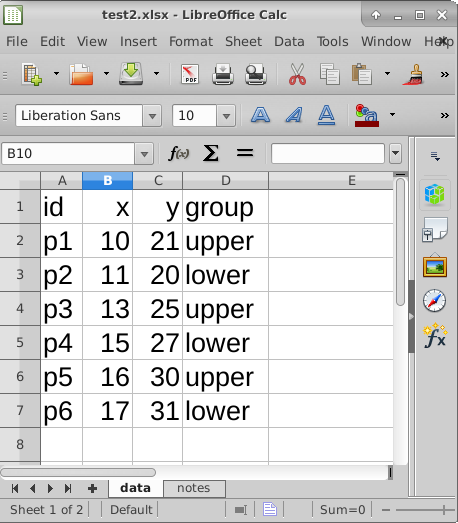
\includegraphics[width=0.4\textwidth]{excel}
\item It is now a workbook with a second sheet called ``notes'' (that
  we don't want).
  \end{itemize}
  
\end{frame}

\begin{frame}[fragile]{Reading it in}
  
  \begin{itemize}
\item Read into R, saying that we only want the sheet ``data''. Start
  with \texttt{file.choose} as before (omitted):
  

\begin{knitrout}
\definecolor{shadecolor}{rgb}{0.969, 0.969, 0.969}\color{fgcolor}\begin{kframe}
\begin{alltt}
\hlkwd{library}\hlstd{(readxl)}
\hlstd{mydata2}\hlkwb{=}\hlkwd{read_excel}\hlstd{(f,}\hlkwc{sheet}\hlstd{=}\hlstr{"data"}\hlstd{)}
\hlstd{mydata2}
\end{alltt}
\begin{verbatim}
## # A tibble: 6 x 4
##      id     x     y group
##   <chr> <dbl> <dbl> <chr>
## 1    p1    10    21 upper
## 2    p2    11    20 lower
## 3    p3    13    25 upper
## 4    p4    15    27 lower
## 5    p5    16    30 upper
## 6    p6    17    31 lower
\end{verbatim}
\end{kframe}
\end{knitrout}
\item That has worked properly.
  \end{itemize}
  
\end{frame}

\begin{frame}[fragile]{Reading Excel spreadsheet into SAS}
  
  \begin{itemize}
  \item Upload the spreadsheet file (as for uploading \texttt{.csv}
    file)
  \item Then, like this:
    
    \begin{Datastep}
proc import 
  datafile='/home/ken/test2.xlsx'
  dbms=xlsx
  out=mydata
  replace;
  sheet=data;
  getnames=yes;
    \end{Datastep}
    
    
  \item \texttt{dbms} is now \texttt{xlsx} for reading this type of
    file (or \texttt{xls} if you have old-style spreadsheet).
  \item Use \texttt{sheet=} to say which worksheet you want (no quotes).
    
  \end{itemize}
  
\end{frame}

\begin{frame}[fragile]{The spreadsheet as data set}

  
  \begin{itemize}
  \item Did it work? Yes:

    \begin{Sascode}[store=re]
proc print;    
  \end{Sascode}
  
  \Listing[store=re]{ree}


  \end{itemize}
  
  
\end{frame}

\begin{frame}[fragile]{Reading Excel files from the Web}
  
  \begin{itemize}
  \item No surprises here.
  \item In R, \texttt{read\_excel} will take a URL rather than a filename,
    in the same way that \texttt{read\_csv} and \texttt{read\_delim}
    do.
  \item In SAS, define a \texttt{filename} as before, and use it in
    the appropriate \texttt{proc import}.
  \end{itemize}
  
\end{frame}

% making graphs


\section{Graphs}

\frame{\sectionpage}

\begin{frame}[fragile]{Our data}
  
  \begin{itemize}
  \item To illustrate making graphs, we need some data.
  \item Data on 202 male and female athletes at the Australian
    Institute of Sport.
  \item Variables:
    \begin{itemize}
    \item categorical: Sex of athlete, sport they play 
    \item quantitative: height (cm), weight (kg), lean body mass, red
      and white blood cell counts, haematocrit and haemoglobin
      (blood), ferritin concentration, body mass index, percent body
      fat. 
    \end{itemize}
  \item Values separated by \emph{tabs} (which impacts reading in).

  \end{itemize}
  
\end{frame}

\begin{frame}[fragile]{Reading data into R}
  

  
  \begin{itemize}
  \item Use \texttt{read\_tsv} (``tab-separated values''), like
    \texttt{read\_csv}.
  \item Data in \texttt{ais.txt}:
    
\begin{knitrout}\small
\definecolor{shadecolor}{rgb}{0.969, 0.969, 0.969}\color{fgcolor}\begin{kframe}
\begin{alltt}
\hlstd{athletes}\hlkwb{=}\hlkwd{read_tsv}\hlstd{(}\hlstr{"ais.txt"}\hlstd{)}
\end{alltt}


{\ttfamily\noindent\itshape\color{messagecolor}{\#\# Parsed with column specification:\\\#\# cols(\\\#\#\ \  Sex = col\_character(),\\\#\#\ \  Sport = col\_character(),\\\#\#\ \  RCC = col\_double(),\\\#\#\ \  WCC = col\_double(),\\\#\#\ \  Hc = col\_double(),\\\#\#\ \  Hg = col\_double(),\\\#\#\ \  Ferr = col\_integer(),\\\#\#\ \  BMI = col\_double(),\\\#\#\ \  SSF = col\_double(),\\\#\#\ \  `\%Bfat` = col\_double(),\\\#\#\ \  LBM = col\_double(),\\\#\#\ \  Ht = col\_double(),\\\#\#\ \  Wt = col\_double()\\\#\# )}}\end{kframe}
\end{knitrout}

  \end{itemize}
  
\end{frame}

\begin{frame}[fragile]{The data (some)}
  
\begin{knitrout}\footnotesize
\definecolor{shadecolor}{rgb}{0.969, 0.969, 0.969}\color{fgcolor}\begin{kframe}
\begin{alltt}
\hlstd{athletes}
\end{alltt}
\begin{verbatim}
## # A tibble: 202 x 13
##       Sex   Sport   RCC   WCC    Hc    Hg  Ferr   BMI   SSF `%Bfat`   LBM
##     <chr>   <chr> <dbl> <dbl> <dbl> <dbl> <int> <dbl> <dbl>   <dbl> <dbl>
##  1 female Netball  4.56  13.3  42.2  13.6    20 19.16  49.0   11.29 53.14
##  2 female Netball  4.15   6.0  38.0  12.7    59 21.15 110.2   25.26 47.09
##  3 female Netball  4.16   7.6  37.5  12.3    22 21.40  89.0   19.39 53.44
##  4 female Netball  4.32   6.4  37.7  12.3    30 21.03  98.3   19.63 48.78
##  5 female Netball  4.06   5.8  38.7  12.8    78 21.77 122.1   23.11 56.05
##  6 female Netball  4.12   6.1  36.6  11.8    21 21.38  90.4   16.86 56.45
##  7 female Netball  4.17   5.0  37.4  12.7   109 21.47 106.9   21.32 53.11
##  8 female Netball  3.80   6.6  36.5  12.4   102 24.45 156.6   26.57 54.41
##  9 female Netball  3.96   5.5  36.3  12.4    71 22.63 101.1   17.93 55.97
## 10 female Netball  4.44   9.7  41.4  14.1    64 22.80 126.4   24.97 51.62
## # ... with 192 more rows, and 2 more variables: Ht <dbl>, Wt <dbl>
\end{verbatim}
\end{kframe}
\end{knitrout}
  
\end{frame}

\begin{frame}[fragile]{Reading data into SAS}
  
  \begin{itemize}
    \item Upload file to SAS Studio first.
  \item A bit trickier because we can't \emph{type} tab: have to use
    special code \texttt{'09'x} (ASCII code \texttt{09} in hex):
    
    \begin{Datastep}
proc import 
  datafile='/home/ken/ais.txt'
  dbms=dlm
  out=sports
  replace;
  delimiter='09'x;
  getnames=yes;

    \end{Datastep}
  \end{itemize}
  
\end{frame}

\begin{frame}[fragile]{Some of the data, tiny}
  
  \begin{Sascode}[store=ga]
proc print data=sports(obs=9);
  \end{Sascode}
  
\Listing[fontsize=scriptsize,store=ga]{gaa}  
  
\end{frame}

\begin{frame}[fragile]{Or, summarized}
  
  \begin{Sascode}[store=gb]
proc means;    
  \end{Sascode}
  
\Listing[store=gb,fontsize=scriptsize]{gbb}  
  
\end{frame}

\begin{frame}[fragile]{Kinds of graph}
  
  Depends on number and type of variables you have:
  
  \begin{center}
  \begin{tabular}{ccp{0.5\textwidth}}
    Categorical & Quantitative & Graph\\
    \hline
    1 & 0 & bar chart\\
    0 & 1 & histogram\\
    2 & 0 & grouped bar charts\\
    1 & 1 & side-by-side boxplots\\
    0 & 2 & scatterplot\\
    2 & 1 & grouped boxplots\\
    1 & 2 & scatterplot with points identified by group (eg.\ by colour)\\
    \hline
  \end{tabular}
    
  \end{center}
  
  With more variables, might want \emph{separate plots by
    groups}. This is called \texttt{facetting} in R, \texttt{paneling}
  in SAS.
  
\end{frame}

\begin{frame}[fragile]{Workhorse graphing procedures}
  
  R and SAS have standard graphing procedures, that we use for all our
  graphs: 
  
  \begin{itemize}
  \item in R, \textbf{ggplot}
  \item in SAS, \textbf{proc sgplot}
  \end{itemize}
  
  Use them in different ways to get precise graph we want.
  
  Let's start with bar chart of the sports played by the athletes.
  
\end{frame}

\begin{frame}[fragile]{Bar chart in R}
  
\begin{knitrout}
\definecolor{shadecolor}{rgb}{0.969, 0.969, 0.969}\color{fgcolor}\begin{kframe}
\begin{alltt}
\hlkwd{ggplot}\hlstd{(athletes,}\hlkwd{aes}\hlstd{(}\hlkwc{x}\hlstd{=Sport))}\hlopt{+}\hlkwd{geom_bar}\hlstd{()}
\end{alltt}
\end{kframe}
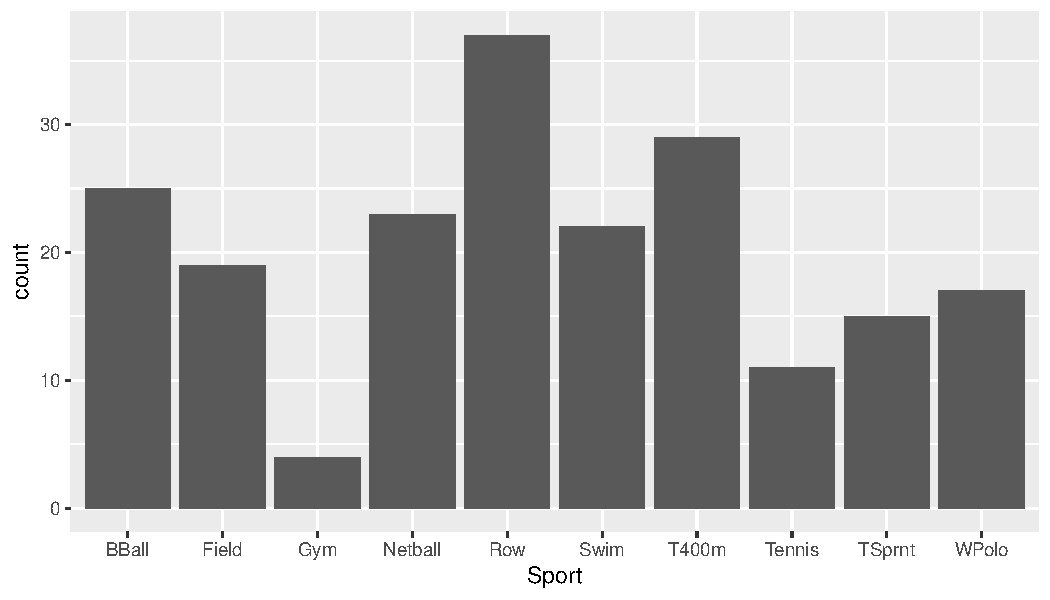
\includegraphics[width=\maxwidth]{figure/unnamed-chunk-27-1} 

\end{knitrout}
  
\end{frame}

\begin{frame}[fragile]{Bar chart in SAS}
  
  \begin{Sascode}[store=gd]
proc sgplot;
  vbar Sport;
  \end{Sascode}
  
  \Graphic[store=gd,scale=0.5]{gdd}
  
\end{frame}

\begin{frame}[fragile]{Histogram of body mass index, in SAS}
  
  \begin{Sascode}[store=ge]
proc sgplot;
  histogram BMI;
  \end{Sascode}
  
  \Graphic[store=ge,scale=0.5]{gee}

  
\end{frame}

\begin{frame}[fragile]{BMI histogram in R}
  
\begin{knitrout}
\definecolor{shadecolor}{rgb}{0.969, 0.969, 0.969}\color{fgcolor}\begin{kframe}
\begin{alltt}
\hlkwd{ggplot}\hlstd{(athletes,}\hlkwd{aes}\hlstd{(}\hlkwc{x}\hlstd{=BMI))}\hlopt{+}\hlkwd{geom_histogram}\hlstd{(}\hlkwc{bins}\hlstd{=}\hlnum{10}\hlstd{)}
\end{alltt}
\end{kframe}
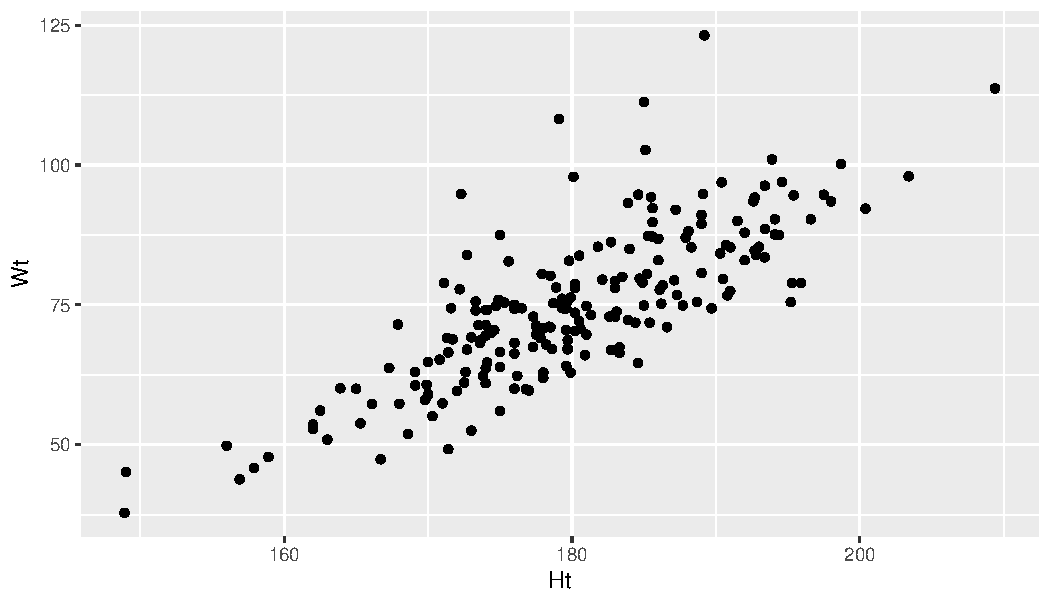
\includegraphics[width=\maxwidth]{figure/unnamed-chunk-28-1} 

\end{knitrout}
  
\end{frame}

\begin{frame}[fragile]{Which sports are played by males and females?}
  

  
\begin{knitrout}
\definecolor{shadecolor}{rgb}{0.969, 0.969, 0.969}\color{fgcolor}\begin{kframe}
\begin{alltt}
\hlkwd{ggplot}\hlstd{(athletes,}\hlkwd{aes}\hlstd{(}\hlkwc{x}\hlstd{=Sport,}\hlkwc{fill}\hlstd{=Sex))}\hlopt{+}
  \hlkwd{geom_bar}\hlstd{(}\hlkwc{position}\hlstd{=}\hlstr{"dodge"}\hlstd{)}
\end{alltt}
\end{kframe}
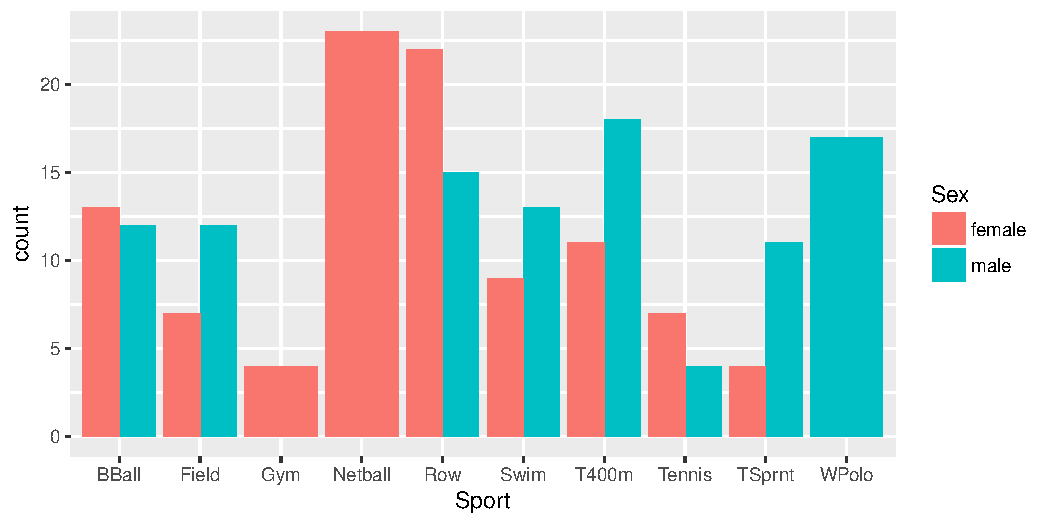
\includegraphics[width=\maxwidth]{figure/unnamed-chunk-29-1} 

\end{knitrout}
  
\end{frame}

\begin{frame}[fragile]{Grouped bar plot in SAS}
  
  \begin{Sascode}[store=gf]
proc sgplot;
  vbar Sport / group=Sex groupdisplay=cluster;
  \end{Sascode}
  
  \Graphic[store=gf,scale=0.5]{gff}
  
\end{frame}

\begin{frame}[fragile]{BMI by gender}
  
  Side-by-side boxplots:
  
  \begin{Sascode}[store=gg]
proc sgplot;
  vbox BMI / category=Sex;
  \end{Sascode}
  
  \Graphic[store=gg,scale=0.5]{ggg}
  
\end{frame}

\begin{frame}[fragile]{And in R}
\begin{knitrout}
\definecolor{shadecolor}{rgb}{0.969, 0.969, 0.969}\color{fgcolor}\begin{kframe}
\begin{alltt}
\hlkwd{ggplot}\hlstd{(athletes,}\hlkwd{aes}\hlstd{(}\hlkwc{x}\hlstd{=Sex,}\hlkwc{y}\hlstd{=BMI))}\hlopt{+}\hlkwd{geom_boxplot}\hlstd{()}
\end{alltt}
\end{kframe}
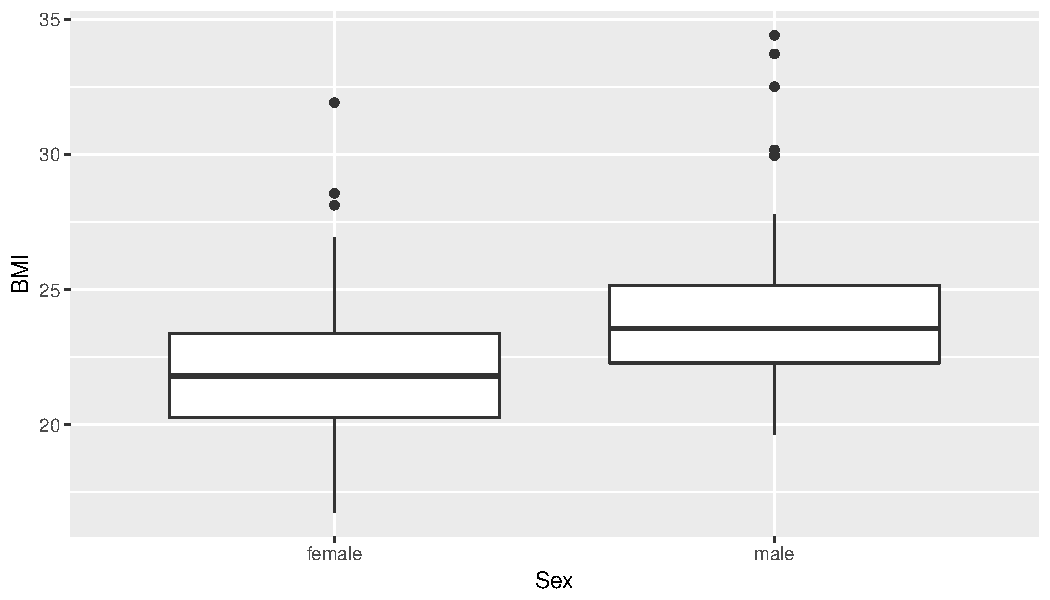
\includegraphics[width=\maxwidth]{figure/unnamed-chunk-30-1} 

\end{knitrout}
\end{frame}

\begin{frame}[fragile]{Height vs.\ weight}
  
  Scatterplot:
  
\begin{knitrout}
\definecolor{shadecolor}{rgb}{0.969, 0.969, 0.969}\color{fgcolor}\begin{kframe}
\begin{alltt}
\hlkwd{ggplot}\hlstd{(athletes,}\hlkwd{aes}\hlstd{(}\hlkwc{x}\hlstd{=Ht,}\hlkwc{y}\hlstd{=Wt))}\hlopt{+}\hlkwd{geom_point}\hlstd{()}
\end{alltt}
\end{kframe}
\includegraphics[width=\maxwidth]{figure/unnamed-chunk-31-1} 

\end{knitrout}
  
\end{frame}

\begin{frame}[fragile]{Height vs.\ weight again}
  
  \begin{Sascode}[store=gh]
proc sgplot;
  scatter x=Ht y=Wt;
  \end{Sascode}
  
  \Graphic[store=gh,scale=0.5]{ghh}
  
\end{frame}

\begin{frame}[fragile]{and again, with regression line}
  
  \begin{Sascode}[store=gj]
proc sgplot;
  scatter x=Ht y=Wt;
  reg x=Ht y=Wt;
  \end{Sascode}
  
  \Graphic[store=gj,scale=0.5]{gjj}
  
  
\end{frame}

\begin{frame}[fragile]{One more time}
  
\begin{knitrout}
\definecolor{shadecolor}{rgb}{0.969, 0.969, 0.969}\color{fgcolor}\begin{kframe}
\begin{alltt}
\hlkwd{ggplot}\hlstd{(athletes,}\hlkwd{aes}\hlstd{(}\hlkwc{x}\hlstd{=Ht,}\hlkwc{y}\hlstd{=Wt))}\hlopt{+}
  \hlkwd{geom_point}\hlstd{()}\hlopt{+}\hlkwd{geom_smooth}\hlstd{(}\hlkwc{method}\hlstd{=}\hlstr{"lm"}\hlstd{)}
\end{alltt}
\end{kframe}
\includegraphics[width=\maxwidth]{figure/unnamed-chunk-32-1} 

\end{knitrout}
  
\end{frame}

\begin{frame}[fragile]{BMI by sport and gender}
  
  \begin{Sascode}[store=gi]
proc sgplot;
  vbox BMI / group=Sex category=Sport;
  \end{Sascode}
  
  \Graphic[store=gi,scale=0.5]{gii}
\end{frame}

\begin{frame}[fragile]{R}
  
\begin{knitrout}
\definecolor{shadecolor}{rgb}{0.969, 0.969, 0.969}\color{fgcolor}\begin{kframe}
\begin{alltt}
\hlkwd{ggplot}\hlstd{(athletes,}\hlkwd{aes}\hlstd{(}\hlkwc{x}\hlstd{=Sport,}\hlkwc{y}\hlstd{=BMI,}\hlkwc{colour}\hlstd{=Sex))}\hlopt{+}
  \hlkwd{geom_boxplot}\hlstd{()}
\end{alltt}
\end{kframe}
\includegraphics[width=\maxwidth]{figure/unnamed-chunk-33-1} 

\end{knitrout}
  
\end{frame}

\begin{frame}[fragile]{Height and weight by gender}

\begin{knitrout}
\definecolor{shadecolor}{rgb}{0.969, 0.969, 0.969}\color{fgcolor}\begin{kframe}
\begin{alltt}
\hlkwd{ggplot}\hlstd{(athletes,}\hlkwd{aes}\hlstd{(}\hlkwc{x}\hlstd{=Ht,}\hlkwc{y}\hlstd{=Wt,}\hlkwc{colour}\hlstd{=Sex))}\hlopt{+}
  \hlkwd{geom_point}\hlstd{()}
\end{alltt}
\end{kframe}
\includegraphics[width=\maxwidth]{figure/unnamed-chunk-34-1} 

\end{knitrout}
  
\end{frame}

\begin{frame}[fragile]{And in SAS}
  
  \begin{Sascode}[store=gk]
proc sgplot;
  scatter x=Ht y=Wt / group=Sex;
  \end{Sascode}
  
  \Graphic[store=gk,scale=0.5]{gkk}
  
\end{frame}

\begin{frame}[fragile]{Height by weight for each sport}
  
  Separate plot for each sport, first two panels here:
  
  \begin{Sascode}[store=gl]
proc sgpanel;
  panelby Sport;
  scatter x=Ht y=Wt / group=Sex;
  \end{Sascode}
  
  \Graphic[store=gl,scale=0.5]{gll}
  
  
\end{frame}

\begin{frame}[fragile]{same in R, with facets}
  
\begin{knitrout}
\definecolor{shadecolor}{rgb}{0.969, 0.969, 0.969}\color{fgcolor}\begin{kframe}
\begin{alltt}
\hlkwd{ggplot}\hlstd{(athletes,}\hlkwd{aes}\hlstd{(}\hlkwc{x}\hlstd{=Ht,}\hlkwc{y}\hlstd{=Wt,}\hlkwc{colour}\hlstd{=Sex))}\hlopt{+}
  \hlkwd{geom_point}\hlstd{()}\hlopt{+}\hlkwd{facet_wrap}\hlstd{(}\hlopt{~}\hlstd{Sport)}
\end{alltt}
\end{kframe}
\includegraphics[width=\maxwidth]{figure/unnamed-chunk-35-1} 

\end{knitrout}
  
  
\end{frame}

\begin{frame}[fragile]{Filling each facet}
  
  Default uses same scale for each facet. To use different scales for
  each facet, this:
  
\begin{knitrout}
\definecolor{shadecolor}{rgb}{0.969, 0.969, 0.969}\color{fgcolor}\begin{kframe}
\begin{alltt}
\hlkwd{ggplot}\hlstd{(athletes,}\hlkwd{aes}\hlstd{(}\hlkwc{x}\hlstd{=Ht,}\hlkwc{y}\hlstd{=Wt,}\hlkwc{colour}\hlstd{=Sex))}\hlopt{+}
  \hlkwd{geom_point}\hlstd{()}\hlopt{+}\hlkwd{facet_wrap}\hlstd{(}\hlopt{~}\hlstd{Sport,}\hlkwc{scales}\hlstd{=}\hlstr{"free"}\hlstd{)}
\end{alltt}
\end{kframe}
\includegraphics[width=\maxwidth]{figure/unnamed-chunk-36-1} 

\end{knitrout}
  
  
\end{frame}

% R scripts


\section{R Studio scripts and projects}

\frame{\sectionpage}

\begin{frame}[fragile]{The console and the script}
  
  \begin{itemize}
  \item You can always type R commands at the console, next to the
    \texttt{>}.
  \item But if you want to use those commands again, or modify them,
    you have to find them first (up/down arrow keys)
  \item plus you have no record of what you did.
  \item Better: create a \emph{script}. File - New File - R Script,
    opens a window top left, into which you can type commands.
  \item To run commands in a script:
    \begin{itemize}
    \item move to or click on the line containing what you want to
      run, then click Run above script window. Runs that line, and
      moves cursor down to next line.
    \item select one or more lines of code, then click Run: runs all
      those lines.
    \end{itemize}
  \end{itemize}
  
\end{frame}

\begin{frame}[fragile]{Advantages of a script}
  
  \begin{itemize}
  \item A script can be \emph{saved} and re-opened later.
  \item This gives you a record of what you did (``reproducible
    research'') 
  \item If something in the script doesn't work, you can fix just
    that part without worrying about the part of the script that works
  \item If you want to run the same code on different data, or
    slightly different code, you can use your script as a starting
    point. (For example, you can keep a bunch of scripts that make
    example plots that you use often.)
  \end{itemize}
  
\end{frame}

\begin{frame}[fragile]{Projects}
  
  \begin{itemize}
  \item A project is a ``container'' for code and data that belong
    together.
  \item Goes with a folder on your computer.
  \item File, New Project. You have option to create the new project
    in a new folder, or in a folder that already exists.
  \item Use a project for a collection of work that belongs together,
    eg.\ data files and code scripts for an assignment. Putting data
    files in a project folder makes it easier to find them.
  \item Later, when we learn about R Markdown, see how to write
    reports that include code. These can go in project folder too.
  \end{itemize}
  
\end{frame}

\begin{frame}[fragile]{Comparison with SAS}
  
  \begin{itemize}
  \item SAS code in SAS Studio \emph{is} a script: some code that is
    saved in a file and can be reloaded and used again.
  \item You can create subfolders under your main folder on SAS
    Studio. These serve the same purpose as R Studio projects: you can
    use them as containers for code, data etc.
  \item Looking ahead, SAS does not have a nice report-writing
    mechanism as R Studio does. (It does have one, \texttt{statrep},
    but that is based on \LaTeX.)
  \end{itemize}
  
\end{frame}

% numerical summaries


\section{More detailed summaries of data}

\frame{\sectionpage}

\begin{frame}[fragile]{Summarizing data in R}


  
  \begin{itemize}
  \item Have seen \texttt{summary} (5-number summary of each
    column). But what if we want:
    
    \begin{itemize}
    \item a summary or two of just one column
    \item a count of observations in each category of a categorical
      variable? 
    \item summaries by group
    \item a different summary of all columns (eg.\ SD)
    \end{itemize}
    
  \item To do this, meet \textbf{pipe} operator \texttt{\%>\%}. This
    takes input data frame, does something do it, and outputs result.
  \item Output from a pipe can be used as input to something else, so
    can have a sequence of pipes.
  \item Summaries include: \texttt{mean}, \texttt{median},
    \texttt{min}, \texttt{max},
    \texttt{sd}, \texttt{IQR}, \texttt{quantile} (for obtaining
    quartiles or any percentile), \texttt{n} (for counting
    observations). 
  \item Use our Australian athletes data again.
  \end{itemize}
  
\end{frame}

\begin{frame}[fragile]{Summarizing one column}
  \begin{itemize}
  \item Like this, for example the mean height:
    
\begin{knitrout}
\definecolor{shadecolor}{rgb}{0.969, 0.969, 0.969}\color{fgcolor}\begin{kframe}
\begin{alltt}
\hlstd{athletes} \hlopt \hlkwd{summarize}\hlstd{(}\hlkwc{m}\hlstd{=}\hlkwd{mean}\hlstd{(Ht))}
\end{alltt}
\begin{verbatim}
## # A tibble: 1 x 1
##         m
##     <dbl>
## 1 180.104
\end{verbatim}
\end{kframe}
\end{knitrout}

or to get mean and SD of BMI:

\begin{knitrout}
\definecolor{shadecolor}{rgb}{0.969, 0.969, 0.969}\color{fgcolor}\begin{kframe}
\begin{alltt}
\hlstd{athletes} \hlopt \hlkwd{summarize}\hlstd{(}\hlkwc{m}\hlstd{=}\hlkwd{mean}\hlstd{(BMI),}\hlkwc{s}\hlstd{=}\hlkwd{sd}\hlstd{(BMI))}
\end{alltt}
\begin{verbatim}
## # A tibble: 1 x 2
##          m        s
##      <dbl>    <dbl>
## 1 22.95589 2.863933
\end{verbatim}
\end{kframe}
\end{knitrout}
  \end{itemize}
\end{frame}

\begin{frame}[fragile]{Quartiles}
  
  \begin{itemize}
  \item \texttt{quantile} calculates percentiles, so we want the 25th
    and 75th percentiles:
    
\begin{knitrout}
\definecolor{shadecolor}{rgb}{0.969, 0.969, 0.969}\color{fgcolor}\begin{kframe}
\begin{alltt}
\hlstd{athletes} \hlopt \hlkwd{summarize}\hlstd{(} \hlkwc{Q1}\hlstd{=}\hlkwd{quantile}\hlstd{(Wt,}\hlnum{0.25}\hlstd{),}
                        \hlkwc{Q3}\hlstd{=}\hlkwd{quantile}\hlstd{(Wt,}\hlnum{0.75}\hlstd{))}
\end{alltt}
\begin{verbatim}
## # A tibble: 1 x 2
##       Q1     Q3
##    <dbl>  <dbl>
## 1 66.525 84.125
\end{verbatim}
\end{kframe}
\end{knitrout}
  \end{itemize}
  
\end{frame}

\begin{frame}[fragile]{Counting how many}
  
  \begin{multicols}{2}
  for example, number of athletes in each sport:
  
\begin{knitrout}
\definecolor{shadecolor}{rgb}{0.969, 0.969, 0.969}\color{fgcolor}\begin{kframe}
\begin{alltt}
\hlstd{athletes} \hlopt \hlkwd{count}\hlstd{(Sport)}
\end{alltt}
\begin{verbatim}
## # A tibble: 10 x 2
##      Sport     n
##      <chr> <int>
##  1   BBall    25
##  2   Field    19
##  3     Gym     4
##  4 Netball    23
##  5     Row    37
##  6    Swim    22
##  7   T400m    29
##  8  Tennis    11
##  9  TSprnt    15
## 10   WPolo    17
\end{verbatim}
\end{kframe}
\end{knitrout}
  
Another way (which will make sense in a moment):

\begin{knitrout}\small
\definecolor{shadecolor}{rgb}{0.969, 0.969, 0.969}\color{fgcolor}\begin{kframe}
\begin{alltt}
\hlstd{athletes} \hlopt \hlkwd{group_by}\hlstd{(Sport)} \hlopt
  \hlkwd{summarize}\hlstd{(}\hlkwc{count}\hlstd{=}\hlkwd{n}\hlstd{())}
\end{alltt}
\begin{verbatim}
## # A tibble: 10 x 2
##      Sport count
##      <chr> <int>
##  1   BBall    25
##  2   Field    19
##  3     Gym     4
##  4 Netball    23
##  5     Row    37
##  6    Swim    22
##  7   T400m    29
##  8  Tennis    11
##  9  TSprnt    15
## 10   WPolo    17
\end{verbatim}
\end{kframe}
\end{knitrout}
    
  \end{multicols}
  
\end{frame}

\begin{frame}[fragile]{Summaries by group}
  
  \begin{itemize}
  \item Might want separate summaries for each ``group'', eg.\ mean
    and SD of height for males and females. Strategy is
    \texttt{group\_by} (to define the groups) and then \texttt{summarize}:
    
\begin{knitrout}
\definecolor{shadecolor}{rgb}{0.969, 0.969, 0.969}\color{fgcolor}\begin{kframe}
\begin{alltt}
\hlstd{athletes} \hlopt \hlkwd{group_by}\hlstd{(Sex)} \hlopt
  \hlkwd{summarize}\hlstd{(}\hlkwc{m}\hlstd{=}\hlkwd{mean}\hlstd{(Ht),}\hlkwc{s}\hlstd{=}\hlkwd{sd}\hlstd{(Ht))}
\end{alltt}
\begin{verbatim}
## # A tibble: 2 x 3
##      Sex        m        s
##    <chr>    <dbl>    <dbl>
## 1 female 174.5940 8.242203
## 2   male 185.5059 7.903487
\end{verbatim}
\end{kframe}
\end{knitrout}

\item This explains second variation on counting within group:
  ``within each sport, how many athletes were there?''
  \end{itemize}
  
\end{frame}

\begin{frame}[fragile]{Summarizing several columns}
  
  \begin{itemize}
  \item Standard deviation of each (numeric) column:
    
\begin{knitrout}\footnotesize
\definecolor{shadecolor}{rgb}{0.969, 0.969, 0.969}\color{fgcolor}\begin{kframe}
\begin{alltt}
\hlstd{athletes} \hlopt \hlkwd{summarize_if}\hlstd{(is.numeric,}\hlkwd{funs}\hlstd{(sd))}
\end{alltt}
\begin{verbatim}
## # A tibble: 1 x 11
##         RCC      WCC       Hc       Hg     Ferr      BMI      SSF  `%Bfat`
##       <dbl>    <dbl>    <dbl>    <dbl>    <dbl>    <dbl>    <dbl>    <dbl>
## 1 0.4579764 1.800549 3.662989 1.362451 47.50124 2.863933 32.56533 6.189826
## # ... with 3 more variables: LBM <dbl>, Ht <dbl>, Wt <dbl>
\end{verbatim}
\end{kframe}
\end{knitrout}

\item Median and IQR of all columns whose name starts with H:
  
\begin{knitrout}
\definecolor{shadecolor}{rgb}{0.969, 0.969, 0.969}\color{fgcolor}\begin{kframe}
\begin{alltt}
\hlstd{athletes} \hlopt \hlkwd{summarize_at}\hlstd{(}\hlkwd{vars}\hlstd{(}\hlkwd{starts_with}\hlstd{(}\hlstr{"H"}\hlstd{)),}
  \hlkwd{funs}\hlstd{(median,IQR))}
\end{alltt}
\begin{verbatim}
## # A tibble: 1 x 6
##   Hc_median Hg_median Ht_median Hc_IQR Hg_IQR Ht_IQR
##       <dbl>     <dbl>     <dbl>  <dbl>  <dbl>  <dbl>
## 1      43.5      14.7     179.7  4.975  2.075 12.175
\end{verbatim}
\end{kframe}
\end{knitrout}
      
  \end{itemize}
  

  
\end{frame}




\begin{frame}[fragile]{Summarizing data in SAS}
  
  \begin{itemize}
  \item Already saw \texttt{proc means} to find means, SDs and sample
    sizes.
  \item \texttt{proc means} will also calculate means of only some
    variables or by group.
  \item Also, \texttt{proc means} can calculate other statistics (by
    group if desired), despite its name.
  \item SAS names for other statistics: \texttt{mean},
    \texttt{median}, \texttt{stddev} (SD), \texttt{qrange} (IQR),
    \texttt{Q1}, \texttt{Q3} (quartiles).
  \end{itemize}
  
\end{frame}

\begin{frame}[fragile]{Specifying summaries, variables and groups}
  
  \begin{itemize}
  \item To specify which summaries to calculate, list them on the
    \texttt{proc means} line.
  \item To specify which variables to calculate summaries for, use a
    line starting with \texttt{var}.
  \item To specify which groups to calculate for, use a line starting
    with \texttt{class} and the name of the grouping variable.
  \item Examples over.

    \begin{Datastep}[program]
data ath;
  set sports;
      \end{Datastep}
    
  \end{itemize}
  
\end{frame}

\begin{frame}[fragile]{Quartiles of athlete weight}
  
  \begin{Sascode}[store=sa]
proc means Q1 Q3 Qrange;
  var Wt;
  \end{Sascode}
  
  \Listing[store=sa,fontsize=small]{saa}
  
\end{frame}

\begin{frame}[fragile]{Mean and SD of height by gender}
  
  \begin{itemize}
  \item Thus:
    
    \begin{Sascode}[store=sb]
proc means mean stddev;
  var Ht;
  class Sex;
    \end{Sascode}
    
    \Listing[store=sb,fontsize=footnotesize]{sbb}
  \end{itemize}
  
\end{frame}

\begin{frame}[fragile]{How many athletes from each sport?}
  
  \begin{itemize}
  \item Have to pick a variable to count observations of (though it
    doesn't matter):
    
    \begin{Sascode}[store=sc]
proc means n;
  var BMI;
  class Sport;
    \end{Sascode}
  \item Results over.
    
  \end{itemize}
  
\end{frame}

\begin{frame}[fragile]{Results}
  
    \Listing[fontsize=scriptsize,store=sc]{scc}
  
  
\end{frame}

\begin{frame}[fragile]{A perhaps better way to count}
  
  \begin{Sascode}[store=sd]
proc freq;
  tables Sport;
  \end{Sascode}
  
  \Listing[fontsize=footnotesize,store=sd]{sdd}
  
\end{frame}


\begin{frame}[fragile]{SD of all the (numerical) columns}
  
  \begin{itemize}
  \item Just don't specify a \texttt{var} or a \texttt{class}:
    
    \begin{Sascode}[store=se]
proc means stddev;
    \end{Sascode}
    
    \Listing[store=se]{see}
  \end{itemize}
  
\end{frame}

% statistical inference


\section{Inference}

\frame{\sectionpage}


\begin{frame}{Statistical Inference and Science}



\begin{itemize}
\item Previously: \emph{descriptive statistics}. ``Here are data; what
  do they say?''.
\item May need to \emph{take some action} based on information in data.
\item Or want to \emph{generalize} beyond data (sample) to larger
  world (population).
\item Science: first guess about how world works.
\item Then collect data, by sampling.
\item Is guess correct (based on data) for whole world, or not?
\end{itemize}

\end{frame}

\begin{frame}[fragile]{Sample data are imperfect}
  
  \begin{itemize}
  \item Sample data never entirely represent what you're observing.
  \item There is always random error present.
  \item Thus you can never be entirely certain about your conclusions.
  \item The Toronto Blue Jays' average home attendance in part of 2015
    season was 25,070
    (up to May 27 2015, from \url{baseball-reference.com}).
  \item Does that mean the attendance at every game was exactly
    25,070? Certainly not. Actual attendance depends on many things, eg.:
    \begin{itemize}
    \item how well the Jays are playing
    \item the opposition
    \item day of week
    \item weather
    \item random chance
    \end{itemize}
  \end{itemize}
  
\end{frame}

\begin{frame}[fragile]{Reading the attendances}

\ldots as a \texttt{.csv} file:

\begin{knitrout}
\definecolor{shadecolor}{rgb}{0.969, 0.969, 0.969}\color{fgcolor}\begin{kframe}
\begin{alltt}
\hlstd{jays}\hlkwb{=}\hlkwd{read_csv}\hlstd{(}\hlstr{"jays15-home.csv"}\hlstd{)}
\end{alltt}


{\ttfamily\noindent\itshape\color{messagecolor}{\#\# Parsed with column specification:\\\#\# cols(\\\#\#\ \  .default = col\_character(),\\\#\#\ \  row = col\_integer(),\\\#\#\ \  game = col\_integer(),\\\#\#\ \  runs = col\_integer(),\\\#\#\ \  Oppruns = col\_integer(),\\\#\#\ \  innings = col\_integer(),\\\#\#\ \  position = col\_integer(),\\\#\#\ \  `game time` = col\_time(format = "{}"{}),\\\#\#\ \  attendance = col\_integer()\\\#\# )}}

{\ttfamily\noindent\itshape\color{messagecolor}{\#\# See spec(...) for full column specifications.}}\end{kframe}
\end{knitrout}
  
\end{frame}

\begin{frame}[fragile]{Taking a look}
  
\begin{knitrout}\footnotesize
\definecolor{shadecolor}{rgb}{0.969, 0.969, 0.969}\color{fgcolor}\begin{kframe}
\begin{alltt}
\hlstd{jays}
\end{alltt}
\begin{verbatim}
## # A tibble: 25 x 21
##      row  game              date      box  team venue   opp result  runs
##    <int> <int>             <chr>    <chr> <chr> <chr> <chr>  <chr> <int>
##  1    82     7    Monday, Apr 13 boxscore   TOR  <NA>   TBR      L     1
##  2    83     8   Tuesday, Apr 14 boxscore   TOR  <NA>   TBR      L     2
##  3    84     9 Wednesday, Apr 15 boxscore   TOR  <NA>   TBR      W    12
##  4    85    10  Thursday, Apr 16 boxscore   TOR  <NA>   TBR      L     2
##  5    86    11    Friday, Apr 17 boxscore   TOR  <NA>   ATL      L     7
##  6    87    12  Saturday, Apr 18 boxscore   TOR  <NA>   ATL   W-wo     6
##  7    88    13    Sunday, Apr 19 boxscore   TOR  <NA>   ATL      L     2
##  8    89    14   Tuesday, Apr 21 boxscore   TOR  <NA>   BAL      W    13
##  9    90    15 Wednesday, Apr 22 boxscore   TOR  <NA>   BAL      W     4
## 10    91    16  Thursday, Apr 23 boxscore   TOR  <NA>   BAL      W     7
## # ... with 15 more rows, and 12 more variables: Oppruns <int>,
## #   innings <int>, wl <chr>, position <int>, gb <chr>, winner <chr>,
## #   loser <chr>, save <chr>, `game time` <time>, Daynight <chr>,
## #   attendance <int>, streak <chr>
\end{verbatim}
\end{kframe}
\end{knitrout}
  
\end{frame}

\begin{frame}[fragile]{Another way}
\begin{knitrout}\scriptsize
\definecolor{shadecolor}{rgb}{0.969, 0.969, 0.969}\color{fgcolor}\begin{kframe}
\begin{alltt}
\hlkwd{glimpse}\hlstd{(jays)}
\end{alltt}
\begin{verbatim}
## Observations: 25
## Variables: 21
## $ row        <int> 82, 83, 84, 85, 86, 87, 88, 89, 90, 91, 92, 93, 94,...
## $ game       <int> 7, 8, 9, 10, 11, 12, 13, 14, 15, 16, 27, 28, 29, 30...
## $ date       <chr> "Monday, Apr 13", "Tuesday, Apr 14", "Wednesday, Ap...
## $ box        <chr> "boxscore", "boxscore", "boxscore", "boxscore", "bo...
## $ team       <chr> "TOR", "TOR", "TOR", "TOR", "TOR", "TOR", "TOR", "T...
## $ venue      <chr> NA, NA, NA, NA, NA, NA, NA, NA, NA, NA, NA, NA, NA,...
## $ opp        <chr> "TBR", "TBR", "TBR", "TBR", "ATL", "ATL", "ATL", "B...
## $ result     <chr> "L", "L", "W", "L", "L", "W-wo", "L", "W", "W", "W"...
## $ runs       <int> 1, 2, 12, 2, 7, 6, 2, 13, 4, 7, 3, 3, 5, 7, 7, 3, 1...
## $ Oppruns    <int> 2, 3, 7, 4, 8, 5, 5, 6, 2, 6, 1, 6, 1, 0, 1, 6, 6, ...
## $ innings    <int> NA, NA, NA, NA, NA, 10, NA, NA, NA, NA, NA, NA, NA,...
## $ wl         <chr> "4-3", "4-4", "5-4", "5-5", "5-6", "6-6", "6-7", "7...
## $ position   <int> 2, 3, 2, 4, 4, 3, 4, 2, 2, 1, 4, 5, 3, 3, 3, 3, 5, ...
## $ gb         <chr> "1", "2", "1", "1.5", "2.5", "1.5", "1.5", "2", "1"...
## $ winner     <chr> "Odorizzi", "Geltz", "Buehrle", "Archer", "Martin",...
## $ loser      <chr> "Dickey", "Castro", "Ramirez", "Sanchez", "Cecil", ...
## $ save       <chr> "Boxberger", "Jepsen", NA, "Boxberger", "Grilli", N...
## $ game time  <time> 02:30:00, 03:06:00, 03:02:00, 03:00:00, 03:09:00, ...
## $ Daynight   <chr> "N", "N", "N", "N", "N", "D", "D", "N", "N", "N", "...
## $ attendance <int> 48414, 17264, 15086, 14433, 21397, 34743, 44794, 14...
## $ streak     <chr> "-", "--", "+", "-", "--", "+", "-", "+", "++", "++...
\end{verbatim}
\end{kframe}
\end{knitrout}
\end{frame}

\begin{frame}[fragile]{Attendance histogram}
\begin{knitrout}
\definecolor{shadecolor}{rgb}{0.969, 0.969, 0.969}\color{fgcolor}\begin{kframe}
\begin{alltt}
\hlkwd{ggplot}\hlstd{(jays,}\hlkwd{aes}\hlstd{(}\hlkwc{x}\hlstd{=attendance))}\hlopt{+}\hlkwd{geom_histogram}\hlstd{(}\hlkwc{bins}\hlstd{=}\hlnum{10}\hlstd{)}
\end{alltt}
\end{kframe}
\includegraphics[width=\maxwidth]{figure/unnamed-chunk-50-1} 

\end{knitrout}

\end{frame}

\begin{frame}[fragile]{Comments}
  
  \begin{itemize}
  \item Attendances have substantial variability, ranging from just
    over 10,000 to around 50,000.
  \item Distribution somewhat skewed to right (but no outliers).
  \item These are a sample of ``all possible games'' (or maybe ``all
    possible games played in April and May''). What can we say about
    mean attendance in all possible games based on this evidence?
  \item Think about:
    \begin{itemize}
    \item Confidence interval
    \item Hypothesis test.
    \end{itemize}
  \end{itemize}
  
\end{frame}



\begin{frame}[fragile]{Getting CI for mean attendance}
  
  \begin{itemize}
  \item \texttt{t.test} function does CI and test. Look at CI first:
\begin{knitrout}
\definecolor{shadecolor}{rgb}{0.969, 0.969, 0.969}\color{fgcolor}\begin{kframe}
\begin{alltt}
\hlkwd{t.test}\hlstd{(jays}\hlopt{$}\hlstd{attendance)}
\end{alltt}
\begin{verbatim}
## 
## 	One Sample t-test
## 
## data:  jays$attendance
## t = 11.389, df = 24, p-value = 3.661e-11
## alternative hypothesis: true mean is not equal to 0
## 95 percent confidence interval:
##  20526.82 29613.50
## sample estimates:
## mean of x 
##  25070.16
\end{verbatim}
\end{kframe}
\end{knitrout}
\item From 20,500 to 29,600.

  \end{itemize}
  
\end{frame}

\begin{frame}[fragile]{Or, 90\% CI}
  
  \begin{itemize}
  \item by including a value for \texttt{conf.level}:
\begin{knitrout}
\definecolor{shadecolor}{rgb}{0.969, 0.969, 0.969}\color{fgcolor}\begin{kframe}
\begin{alltt}
\hlkwd{t.test}\hlstd{(jays}\hlopt{$}\hlstd{attendance,}\hlkwc{conf.level}\hlstd{=}\hlnum{0.90}\hlstd{)}
\end{alltt}
\begin{verbatim}
## 
## 	One Sample t-test
## 
## data:  jays$attendance
## t = 11.389, df = 24, p-value = 3.661e-11
## alternative hypothesis: true mean is not equal to 0
## 90 percent confidence interval:
##  21303.93 28836.39
## sample estimates:
## mean of x 
##  25070.16
\end{verbatim}
\end{kframe}
\end{knitrout}
\item From 21,300 to 28,800. (Shorter, as it should be.)
  \end{itemize}
  
\end{frame}
\begin{frame}[fragile]{Comments}
  
  \begin{itemize}
  \item Need to say ``column \texttt{attendance} within data frame
    \texttt{jays}'' using \texttt{\$}.
  \item 95\% CI from about 20,000 to about 30,000.
  \item Not estimating mean  attendance well at all!
  \item Generally want confidence interval to be \emph{shorter}, which
    happens if:
    \begin{itemize}
    \item SD smaller
    \item sample size \emph{bigger}
    \item confidence level smaller
    \end{itemize}
  \item Last one is a cheat, really, since reducing confidence level
    increases chance that interval won't contain pop.\ mean at all!
  \end{itemize}
  
\end{frame}

\begin{frame}[fragile]{Another way to access data frame columns}
  
\begin{knitrout}
\definecolor{shadecolor}{rgb}{0.969, 0.969, 0.969}\color{fgcolor}\begin{kframe}
\begin{alltt}
\hlkwd{with}\hlstd{(jays,}\hlkwd{t.test}\hlstd{(attendance))}
\end{alltt}
\begin{verbatim}
## 
## 	One Sample t-test
## 
## data:  attendance
## t = 11.389, df = 24, p-value = 3.661e-11
## alternative hypothesis: true mean is not equal to 0
## 95 percent confidence interval:
##  20526.82 29613.50
## sample estimates:
## mean of x 
##  25070.16
\end{verbatim}
\end{kframe}
\end{knitrout}
  
\end{frame}

\begin{frame}[fragile]{Hypothesis test}
  
  \begin{itemize}
  \item CI answers question ``what is the mean?''
  \item Might have a value $\mu$ in mind for the mean, and question
    ``Is the mean equal to $\mu$, or not?''
  \item For example, 2014 average attendance was 29,327. 
  \item Second question answered by \textbf{hypothesis test}.
  \item Value being assessed goes in \textbf{null hypothesis}: here,
    $H_0: \mu=29,327$.
  \item \textbf{Alternative hypothesis} says how null might be wrong,
    eg.\ $H_a: \mu \ne 29,327$.
  \item Assess evidence \emph{against null}. If that evidence strong
    enough, \emph{reject null hypothesis}; if not, \emph{fail to
      reject null hypothesis} (sometimes \emph{retain null}). 
  \item Note asymmetry between null and alternative, and utter absence
    of word ``accept''. 
  \end{itemize}
  
\end{frame}

\begin{frame}[fragile]{$\alpha$ and errors}
  
  \begin{itemize}
  \item Hypothesis test ends with \emph{decision}:
    \begin{itemize}
    \item reject null hypothesis
    \item do not reject null hypothesis.
    \end{itemize}
  \item but decision may be \emph{wrong}:
    

\begin{center}
  
  
\begin{tabular}{|l|cc|}
\hline
  & \multicolumn{2}{c|}{Decision}\\
Truth & Do not reject & Reject null\\
\hline
Null true & Correct & Type I error\\
Null false & Type II error & Correct\\
\hline
\end{tabular}
\end{center}

\item Either type of error is bad, but for now focus on controlling
  Type I error: write $\alpha=P(\mbox{type I error})$, and devise test
  so that $\alpha$ \emph{small}, typically 0.05.
\item That is, \textbf{if null hypothesis true}, have only small
  chance to reject it (which would be a mistake).
\item Worry about type II errors later (when we consider power of
  test). 

  \end{itemize}
  
\end{frame}

\begin{frame}[fragile]{Why 0.05? This man.}
  
  \begin{multicols}{2}
  
  \includegraphics[width=2in]{fisher}
  
  Responsible for:
  
  \begin{itemize}
  \item analysis of variance
  \item Fisher information
  \item Linear discriminant analysis
  \item Fisher's $z$-transformation
  \item Fisher-Yates shuffle
  \item Behrens-Fisher problem
  \end{itemize}

  Sir Ronald A.\ Fisher, 1890--1962.
  \end{multicols}
  
\end{frame}

\begin{frame}[fragile]{Why 0.05? (2)}
  
  \begin{itemize}
  \item From \emph{The Arrangement of Field Experiments}
    (1926):
    
    \includegraphics[width=0.9\textwidth]{fisher1}
    
  \item and
    
    \includegraphics[width=0.9\textwidth]{fisher2}
  \end{itemize}
  
\end{frame}

\begin{frame}[fragile]{Test statistic: going from data to decision}
  
  \begin{itemize}
  \item ``How far away from null hypothesis is data?''
  \item In testing for mean, statistic is
    $$ t = { \bar{x} - \mu \over s/\sqrt{n} }$$
  \item and for our baseball attendance data
\begin{knitrout}
\definecolor{shadecolor}{rgb}{0.969, 0.969, 0.969}\color{fgcolor}\begin{kframe}
\begin{alltt}
\hlstd{t.stat}\hlkwb{=}\hlstd{(}\hlnum{25070}\hlopt{-}\hlnum{29327}\hlstd{)}\hlopt{/}\hlstd{(}\hlnum{11000}\hlopt{/}\hlkwd{sqrt}\hlstd{(}\hlnum{25}\hlstd{))}
\hlstd{t.stat}
\end{alltt}
\begin{verbatim}
## [1] -1.935
\end{verbatim}
\end{kframe}
\end{knitrout}

  \end{itemize}
  
\end{frame}

\begin{frame}[fragile]{P-value}
  
  \begin{itemize}
  \item The probability of observing a test statistic value \emph{as
      extreme or more extreme than that observed, if the null
      hypothesis is true}.
  \item ``More extreme'' depends on $H_a$: count both sides if
    two-sided, count only the proper side if one-sided.
  \item Our $H_a$ was $H_a:  \mu \ne 29,327$, two-sided.
  \end{itemize}
  
\end{frame}


\begin{frame}[fragile]{$t$-table}
  
  \begin{multicols}{2}

      \includegraphics[height=0.95\textheight]{StudentTTable}

      \begin{itemize}
      \item $n=25$ so df is $25-1=24$.
      \item Look up 1.935 not $-1.935$.
      \item $1.71 < 1.935 < 2.06$
      \item P-value between 0.05 and 0.10

\item P-value not less than 0.05: do not reject null.
\item No evidence of change in mean attendance.
      \end{itemize}
    
  \end{multicols}
  
  
\end{frame}


\begin{frame}[fragile]{Or, again, using \texttt{t.test}:}
  
\begin{knitrout}
\definecolor{shadecolor}{rgb}{0.969, 0.969, 0.969}\color{fgcolor}\begin{kframe}
\begin{alltt}
\hlkwd{t.test}\hlstd{(jays}\hlopt{$}\hlstd{attendance,} \hlkwc{mu}\hlstd{=}\hlnum{29327}\hlstd{)}
\end{alltt}
\begin{verbatim}
## 
## 	One Sample t-test
## 
## data:  jays$attendance
## t = -1.9338, df = 24, p-value = 0.06502
## alternative hypothesis: true mean is not equal to 29327
## 95 percent confidence interval:
##  20526.82 29613.50
## sample estimates:
## mean of x 
##  25070.16
\end{verbatim}
\end{kframe}
\end{knitrout}

  
  \begin{itemize}
  \item See test statistic $-1.93$, P-value 0.065.
  \item Again, do not reject null: conclusion same.
  \end{itemize}
  
\end{frame}


\begin{frame}[fragile]{And in SAS}
  
  \begin{Datastep}
proc import
  datafile='/home/ken/jays15-home.csv'
    dbms=csv
    out=jays
    replace;
  getnames=yes;
  \end{Datastep}
  
\end{frame}

\begin{frame}[fragile]{Checking what I read in}
  
  \begin{itemize}
  \item Especially important in SAS:
    
    \begin{Sascode}[store=iza]
proc print data=jays(obs=6);      
    \end{Sascode}
    
    \Listing[fontsize=tiny,store=iza]{izaa}
  \end{itemize}
  
\end{frame}

\begin{frame}[fragile]{Doing the $t$-test}
  \begin{Sascode}[store=ia]
proc ttest h0=29327;
  var attendance;
  \end{Sascode}

  \Listing[store=ia,fontsize=small]{iaa}
  
  Same CI (20527 to 29614) as R, also same P-value 0.0650.

\end{frame}



\begin{frame}[fragile]{Day and night games}
  
  \begin{itemize}
  \item \texttt{daynight} is \texttt{D} for a day game and \texttt{N} for
    a night game. How do attendances compare for these?
\begin{Sascode}[store=id]
  proc sgplot;
    vbox attendance / category=daynight;
\end{Sascode}
  \end{itemize}
  
\end{frame}

\begin{frame}[fragile]{The boxplot}
  
\Graphic[scale=0.5,store=id]{idd}
  
\end{frame}


\begin{frame}[fragile]{Comments}
  
  \begin{itemize}
  \item Attendances on average \emph{much} higher for day games than
    night ones.
  \item Why?
  \item What is that upper outlier in the night games?
  \end{itemize}
  
\end{frame}

%\begin{frame}[fragile]{Inference for proportions}
%  
%  \begin{itemize}
%  \item An instant coffee company took a random sample of 100 married
%    men, and found that 20 of the men in the sample preferred that
%    brand of coffee. What can we say about the proportion of all
%    married men that would prefer that brand of coffee?
%    
%  \item Also, is there evidence that the proportion of all married men
%    preferring that brand is greater than 0.15?
%    
%  \item \texttt{prop.test}.
%  
%  \end{itemize}
%  
%\end{frame}
%
%
%\begin{frame}[fragile]{Confidence interval}
%
%\begin{Rcode}
%prop.test(20,100)  
%\end{Rcode}
%
%0.13 to 0.29. Ignore P-value.
%  
%\end{frame}
%
%\begin{frame}[fragile]{and then test}
%
%\begin{Rcode}
%prop.test(20,100,p=0.15,alternative="greater")  
%\end{Rcode}
%
%P-value $0.1038>0.05$, no evidence that proportion greater than
%0.15. (Sample proportion would have to be much bigger, or sample size larger.)
%
%Ignore CI (``one-sided CI''). 
%  
%\end{frame}


\begin{frame}{Another example: learning to read}

  \begin{itemize}
  \item You devised new method for teaching children to read.
  \item Guess it will be more effective than current methods.
  \item To support this guess, collect data.
  \item Want to generalize to ``all children in Canada''.
  \item So take random sample of all children in Canada.
  \item Or, argue that sample you actually have is ``typical'' of all
    children in Canada.
  \item Randomization: whether or not a child in sample or not has
    nothing to do with anything else about that child.
  \item Aside: if your new method good for 
    teaching \emph{struggling} children to read, then ``all
    kids'' is ``all kids having trouble learning to
    read'', and you take a sample of \emph{those}.
  \end{itemize}
  
\end{frame}

\begin{frame}[fragile]{The data (some), in SAS}

  \begin{itemize}
    \item Data in file \texttt{drp.txt} with header line, group then
    reading test score, separated by \emph{space}:
  \end{itemize}

\begin{Datastep}
proc import
  datafile='/home/ken/drp.txt'
  dbms=dlm
  out=reading
  replace;
  delimiter=' ';
  getnames=yes;
\end{Datastep}
%$ %$
\begin{Sascode}[store=ix]
  proc print;
\end{Sascode}
  
\end{frame}


\begin{frame}[fragile]{The data, some, tiny}

  \Listing[store=ix,fontsize=tiny]{ixx}
  
\end{frame}


\begin{frame}[fragile]{Analysis}

  \begin{itemize}
    \item Groups labelled \texttt{c} for ``control'' and \texttt{t}
      for ``treatment''.
    \item Start with summaries (group means) and plot (boxplot).
  \item No pairing, matching: might compare means with \emph{two-sample $t$-test}.
  \item For test, need approx.\ normality, but don't need equal variability.
    \item Use summaries to decide if test reasonable.

  \end{itemize}
  
\end{frame}

\begin{frame}[fragile]{Comparing means}

\begin{Sascode}[store=if]
  proc means;
    class group;
    var score;
\end{Sascode}

\Listing[store=if,fontsize=scriptsize]{iff}
  
\end{frame}

\begin{frame}[fragile]{Boxplots}

\begin{Sascode}[store=ifx]
  proc sgplot;
    vbox score / category=group;
\end{Sascode}

\Graphic[store=ifx,scale=0.5]{ifxx}

  
\end{frame}

\begin{frame}{Comments}

\begin{itemize}
\item Groups not actually same size (maybe 2 kids had to drop out).
\item Means a fair bit different, treatment mean higher.
\item But a lot of variability, so groups do overlap.
\item Standard deviations somewhat different too.
  \item Biggest threat to normality is outliers, none here.
  \item Both distributions not far off symmetric.
  \item $t$-test should be good enough.
  \end{itemize}
  
\end{frame}

\begin{frame}[fragile]{The $t$-test}

\begin{Sascode}[store=ihy]
  proc ttest side=L;
    var score;
    class group;
\end{Sascode}

\Listing[store=ihy,objects=ttests,fontsize=small]{ihyy}

plus a lot more output. 



\end{frame}

\begin{frame}{Comments and Conclusions}

  \begin{itemize}
  \item One-sided test (looking for \emph{improvement}). \texttt{side}
    can be \texttt{L} (lower), \texttt{U} (upper) or \texttt{2}
    (two-sided, can be omitted.) This is \texttt{L} because control
    group first in alphabetical order.
  \item Right $t$-test is Satterthwaite (does not assume equal variability)
  \item P-value $0.0132<0.05$: there \emph{is} increase in reading scores.
  \item Should not use pooled test, because SDs not close; even so,
    result very similar (P-value 0.0143).
  \item One-sided test doesn't give (regular) CI for difference in
    means. To get that, repeat analysis without \texttt{side=L}.
  \end{itemize}
  
\end{frame}

\begin{frame}[fragile]{Doing it with R}

  \begin{itemize}
  \item Proper reading-in function is \texttt{read\_delim}.
  \item If you know that the file is in current folder, read it in by
    name (instead of searching for it):
    
\begin{knitrout}
\definecolor{shadecolor}{rgb}{0.969, 0.969, 0.969}\color{fgcolor}\begin{kframe}
\begin{alltt}
\hlstd{kids}\hlkwb{=}\hlkwd{read_delim}\hlstd{(}\hlstr{"drp.txt"}\hlstd{,}\hlstr{" "}\hlstd{)}
\end{alltt}


{\ttfamily\noindent\itshape\color{messagecolor}{\#\# Parsed with column specification:\\\#\# cols(\\\#\#\ \  group = col\_character(),\\\#\#\ \  score = col\_integer()\\\#\# )}}\end{kframe}
\end{knitrout}


  \end{itemize}
  
\end{frame}


\begin{frame}[fragile]{The data}
  
\begin{knitrout}\small
\definecolor{shadecolor}{rgb}{0.969, 0.969, 0.969}\color{fgcolor}\begin{kframe}
\begin{alltt}
\hlstd{kids}
\end{alltt}
\begin{verbatim}
## # A tibble: 44 x 2
##    group score
##    <chr> <int>
##  1     t    24
##  2     t    61
##  3     t    59
##  4     t    46
##  5     t    43
##  6     t    44
##  7     t    52
##  8     t    43
##  9     t    58
## 10     t    67
## # ... with 34 more rows
\end{verbatim}
\end{kframe}
\end{knitrout}
  
\end{frame}

\begin{frame}[fragile]{Boxplots}
  
\begin{knitrout}
\definecolor{shadecolor}{rgb}{0.969, 0.969, 0.969}\color{fgcolor}\begin{kframe}
\begin{alltt}
\hlkwd{ggplot}\hlstd{(kids,}\hlkwd{aes}\hlstd{(}\hlkwc{x}\hlstd{=group,}\hlkwc{y}\hlstd{=score))}\hlopt{+}\hlkwd{geom_boxplot}\hlstd{()}
\end{alltt}
\end{kframe}
\includegraphics[width=\maxwidth]{figure/unnamed-chunk-58-1} 

\end{knitrout}
  
\end{frame}

\begin{frame}[fragile]{The (Satterthwaite-Welch) $t$-test}
  
  \begin{itemize}
  \item \texttt{c} (control) before \texttt{t} (treatment)
    alphabetically, so proper alternative is ``less''.
  \item R does Satterthwaite test by default (as before: new reading program really helps):


\begin{knitrout}\footnotesize
\definecolor{shadecolor}{rgb}{0.969, 0.969, 0.969}\color{fgcolor}\begin{kframe}
\begin{alltt}
\hlkwd{t.test}\hlstd{(score}\hlopt{~}\hlstd{group,}\hlkwc{data}\hlstd{=kids,}\hlkwc{alternative}\hlstd{=}\hlstr{"less"}\hlstd{)}
\end{alltt}
\begin{verbatim}
## 
## 	Welch Two Sample t-test
## 
## data:  score by group
## t = -2.3109, df = 37.855, p-value = 0.01319
## alternative hypothesis: true difference in means is less than 0
## 95 percent confidence interval:
##       -Inf -2.691293
## sample estimates:
## mean in group c mean in group t 
##        41.52174        51.47619
\end{verbatim}
\end{kframe}
\end{knitrout}
  \end{itemize}
  
\end{frame}

\begin{frame}[fragile]{The pooled $t$-test}

  \begin{itemize}
  \item Pooled (equal variances) test this way:

\begin{knitrout}
\definecolor{shadecolor}{rgb}{0.969, 0.969, 0.969}\color{fgcolor}\begin{kframe}
\begin{alltt}
\hlkwd{t.test}\hlstd{(score}\hlopt{~}\hlstd{group,}\hlkwc{data}\hlstd{=kids,}\hlkwc{alternative}\hlstd{=}\hlstr{"less"}\hlstd{,}
  \hlkwc{var.equal}\hlstd{=T)}
\end{alltt}
\begin{verbatim}
## 
## 	Two Sample t-test
## 
## data:  score by group
## t = -2.2666, df = 42, p-value = 0.01431
## alternative hypothesis: true difference in means is less than 0
## 95 percent confidence interval:
##       -Inf -2.567497
## sample estimates:
## mean in group c mean in group t 
##        41.52174        51.47619
\end{verbatim}
\end{kframe}
\end{knitrout}

\item Similar P-value to Satterthwaite test (and same results as SAS).
  \end{itemize}
  
\end{frame}

\begin{frame}[fragile]{Two-sided test; CI}
  
  \begin{itemize}
\item To do 2-sided test, leave out \texttt{alternative}:

  {\small
\begin{knitrout}
\definecolor{shadecolor}{rgb}{0.969, 0.969, 0.969}\color{fgcolor}\begin{kframe}
\begin{alltt}
\hlkwd{t.test}\hlstd{(score}\hlopt{~}\hlstd{group,}\hlkwc{data}\hlstd{=kids)}
\end{alltt}
\begin{verbatim}
## 
## 	Welch Two Sample t-test
## 
## data:  score by group
## t = -2.3109, df = 37.855, p-value = 0.02638
## alternative hypothesis: true difference in means is not equal to 0
## 95 percent confidence interval:
##  -18.67588  -1.23302
## sample estimates:
## mean in group c mean in group t 
##        41.52174        51.47619
\end{verbatim}
\end{kframe}
\end{knitrout}
}

\item Also gives CI: new reading program increases average scores by somewhere
  between about 1 and 19 points. 
\item Confidence intervals inherently two-sided, so do 2-sided test to
  get them.

  \end{itemize}

\end{frame}

%\begin{frame}{Jargon for testing}
%
%  \begin{description}
%  \item[Alternative hypothesis:] what we are trying to prove (new reading
%    program is effective).
%  \item[Null hypothesis:] ``there is no difference'' (new reading program
%    no better than current program). \emph{Must contain ``equals''}.
%  \item[One-sided alternative:] trying to prove \emph{better} (as with
%    reading program).
%  \item[Two-sided alternative:] trying to prove \emph{different}.
%  \item[Test statistic:] something expressing difference between data
%    and null (eg.\ difference in sample means, $t$ statistic).
%  \item[P-value:] probability of observing test statistic value
%    \emph{as extreme or more extreme, if null is true}.
%  \end{description}
%  
%\end{frame}

\begin{frame}{Logic of testing}

  \begin{itemize}
  \item Work out what \emph{would} happen if null hypothesis were true.
  \item Compare to what actually \emph{did} happen.
  \item If these are too far apart, conclude that null hypothesis
    \emph{is not} true after all. (Be guided by P-value.)
  \end{itemize}

As applied to our reading programs:

\begin{itemize}
\item If reading programs equally good, expect to see a difference in
  means close to 0. 
  \begin{itemize}
  \item Closeness quantified eg.\ by $t$.
  \end{itemize}
\item Mean reading score was 10 higher for new program.
\item Difference of 10 was unusually big (P-value small from
  $t$-test). So conclude that new reading program is effective.
\end{itemize}

Nothing here about what happens if null hypothesis is
\emph{false}. This is power and type II error probability.
  
\end{frame}

\begin{frame}{Errors in testing}

What can happen:

\bigskip

\begin{center}
\begin{tabular}{|l|cc|}
\hline
  & \multicolumn{2}{c|}{Decision}\\
Truth & Do not reject & Reject null\\
\hline
Null true & Correct & Type I error\\
Null false & Type II error & Correct\\
\hline
\end{tabular}  
\end{center}

\bigskip

Tension between \emph{truth} and \emph{decision about truth}
(imperfect). 

\begin{itemize}
\item Prob.\ of type I error denoted $\alpha$. Usually fix $\alpha$,
  eg.\ $\alpha=0.05$.
\item Prob.\ of type II error denoted $\beta$. Determined by the planned
  experiment. Low $\beta$ good.
\item Prob.\ of \emph{not} making type II error called \textbf{power}
  ($=1-\beta)$. \emph{High} power good.
\end{itemize}
  
\end{frame}

  


\begin{frame}[fragile]{Power}
  \begin{itemize}
  \item Suppose $H_0: \theta=10$, $H_a: \theta \ne 10$ for some
    parameter $\theta$.
  \item Suppose $H_0$ wrong. What does that say about $\theta$?
  \item Not much. Could have $\theta=11$ or $\theta=8$ or
    $\theta=496$. In each case, $H_0$ wrong.
  \item How likely a type II error is depends on what $\theta$ is:
    \begin{itemize}
    \item If $\theta=496$, should be able to reject $H_0:\theta=10$
      even for small sample, so $\beta$ should be small (power large).
    \item If $\theta=11$, might have hard time rejecting $H_0$ even
      with large sample, so $\beta$ would be larger (power smaller).
    \end{itemize}
  \item \emph{Power depends on true parameter value, and on sample size.}
  \item So we play ``what if'': ``if $\theta$ were 11 (or 8 or 496),
    what would power be?''.
  \end{itemize}
\end{frame}

\begin{frame}{Figuring out power}

  \begin{itemize}
  \item Time to figure out power is \emph{before} you collect any
    data, as part of planning process.
  \item Need to have idea of what kind of departure from null
    hypothesis of interest to you, eg.\ average improvement of 5 points on
    reading test scores. (Subject-matter decision, not statistical one.)
  \item Then, either:
    \begin{itemize}
    \item ``I have this big a sample and this big a departure I want
      to detect. What is my power for detecting it?''
    \item ``I want to detect this big a departure with this much
      power. How big a sample size do I need?''
    \end{itemize}
  \item R or SAS.
  \end{itemize}
  
\end{frame}

\begin{frame}[fragile]{How to understand/estimate power?}
  
  \begin{itemize}
  \item Suppose we test $H_0: \mu=10$ against $H_a: \mu \ne 10$, where
    $\mu$ is population mean.
  \item Suppose in actual fact, $\mu=8$, so $H_0$ is \emph{wrong}. We
    want to reject it. How likely is that to happen?
  \item Need population SD (take $\sigma=4$) and sample size (take
    $n=15$). In practice, get $\sigma$ from pilot/previous study, and
    take the $n$ we plan to use.
  \item Idea: draw a random sample from the \emph{true} distribution,
    test whether its mean is 10 or not.
  \item Repeat previous step ``many'' times.
    
  \item ``Simulation''.
  \item Most easily in R.
  \end{itemize}
\end{frame}

\begin{frame}[fragile]{Making it go}
  
  \begin{itemize}
  \item Random sample of 15 normal observations with mean 8 and SD 4:


\begin{knitrout}\small
\definecolor{shadecolor}{rgb}{0.969, 0.969, 0.969}\color{fgcolor}\begin{kframe}
\begin{alltt}
\hlstd{x}\hlkwb{=}\hlkwd{rnorm}\hlstd{(}\hlnum{15}\hlstd{,}\hlnum{8}\hlstd{,}\hlnum{4}\hlstd{)}
\hlstd{x}
\end{alltt}
\begin{verbatim}
##  [1] 14.487469  5.014611  6.924277  5.201860  8.852952 10.835874  3.686684
##  [8] 11.165242  8.016188 12.383518  1.378099  3.172503 13.074996 11.353573
## [15]  5.015575
\end{verbatim}
\end{kframe}
\end{knitrout}
\item Test whether \texttt{x} from population with mean 10 or not:
\begin{knitrout}\small
\definecolor{shadecolor}{rgb}{0.969, 0.969, 0.969}\color{fgcolor}\begin{kframe}
\begin{alltt}
\hlkwd{t.test}\hlstd{(x,}\hlkwc{mu}\hlstd{=}\hlnum{10}\hlstd{)}
\end{alltt}
\begin{verbatim}
## 
## 	One Sample t-test
## 
## data:  x
## t = -1.8767, df = 14, p-value = 0.08157
## alternative hypothesis: true mean is not equal to 10
## 95 percent confidence interval:
##   5.794735 10.280387
## sample estimates:
## mean of x 
##  8.037561
\end{verbatim}
\end{kframe}
\end{knitrout}
  
  \end{itemize}
  
\end{frame}

\begin{frame}[fragile]{\ldots continued}
  
  \begin{itemize}
   
\item Fail to reject the mean being 10 (a Type II error).    
\item Same again, but just get the P-value:
  
\begin{knitrout}
\definecolor{shadecolor}{rgb}{0.969, 0.969, 0.969}\color{fgcolor}\begin{kframe}
\begin{alltt}
\hlkwd{t.test}\hlstd{(x,}\hlkwc{mu}\hlstd{=}\hlnum{10}\hlstd{)}\hlopt{$}\hlstd{p.value}
\end{alltt}
\begin{verbatim}
## [1] 0.0815652
\end{verbatim}
\end{kframe}
\end{knitrout}
  \end{itemize}
  
\end{frame}

\begin{frame}[fragile]{Write a function\ldots}
  
  \begin{itemize}
  \item \ldots to generate the random sample and return its P-value:
    
\begin{knitrout}
\definecolor{shadecolor}{rgb}{0.969, 0.969, 0.969}\color{fgcolor}\begin{kframe}
\begin{alltt}
\hlstd{sim}\hlkwb{=}\hlkwa{function}\hlstd{() \{}
  \hlstd{x}\hlkwb{=}\hlkwd{rnorm}\hlstd{(}\hlnum{15}\hlstd{,}\hlnum{8}\hlstd{,}\hlnum{4}\hlstd{)}
  \hlkwd{t.test}\hlstd{(x,}\hlkwc{mu}\hlstd{=}\hlnum{10}\hlstd{)}\hlopt{$}\hlstd{p.value}
\hlstd{\}}
\end{alltt}
\end{kframe}
\end{knitrout}

\item Test it (different from before: random data):
  
\begin{knitrout}
\definecolor{shadecolor}{rgb}{0.969, 0.969, 0.969}\color{fgcolor}\begin{kframe}
\begin{alltt}
\hlkwd{sim}\hlstd{()}
\end{alltt}
\begin{verbatim}
## [1] 0.1286652
\end{verbatim}
\end{kframe}
\end{knitrout}

\item Once again fail to reject a null mean of 10 (incorrectly).
  \end{itemize}
  
\end{frame}

\begin{frame}[fragile]{To run lots of times}
  
  \begin{itemize}
  \item Like this --- ``as many times as the first thing, do the second thing'':
\begin{knitrout}
\definecolor{shadecolor}{rgb}{0.969, 0.969, 0.969}\color{fgcolor}\begin{kframe}
\begin{alltt}
\hlstd{pvals}\hlkwb{=}\hlkwd{replicate}\hlstd{(}\hlnum{1000}\hlstd{,}\hlkwd{sim}\hlstd{())}
\hlkwd{head}\hlstd{(pvals)}
\end{alltt}
\begin{verbatim}
## [1] 0.189800019 0.000728556 0.250217788 0.277753581 0.014665480 0.160853544
\end{verbatim}
\end{kframe}
\end{knitrout}
\item What fraction of those P-values are 0.05 or smaller? This is our
  best guess at how often our test will correctly reject:
  
\begin{knitrout}
\definecolor{shadecolor}{rgb}{0.969, 0.969, 0.969}\color{fgcolor}\begin{kframe}
\begin{alltt}
\hlkwd{table}\hlstd{(pvals}\hlopt{<=}\hlnum{0.05}\hlstd{)}
\end{alltt}
\begin{verbatim}
## 
## FALSE  TRUE 
##   578   422
\end{verbatim}
\end{kframe}
\end{knitrout}

\item Test correctly rejects 422 times of 1000: estimated power is 0.422.
  \end{itemize}
  
\end{frame}


\begin{frame}[fragile]{Calculating power}
  
  \begin{itemize}
  \item Simulation approach very flexible: will work for any test. But
    answer different each time because of randomness.
  \item In some cases, for example 1-sample and 2-sample $t$-tests,
    power can be \emph{calculated}.
  \item In R, \texttt{power.t.test}. \texttt{delta} is
    \emph{difference} between null and true mean:
    
\begin{knitrout}
\definecolor{shadecolor}{rgb}{0.969, 0.969, 0.969}\color{fgcolor}\begin{kframe}
\begin{alltt}
\hlkwd{power.t.test}\hlstd{(}\hlkwc{n}\hlstd{=}\hlnum{15}\hlstd{,}\hlkwc{delta}\hlstd{=}\hlnum{2}\hlstd{,}\hlkwc{sd}\hlstd{=}\hlnum{4}\hlstd{,}\hlkwc{type}\hlstd{=}\hlstr{"one.sample"}\hlstd{)}
\end{alltt}
\begin{verbatim}
## 
##      One-sample t test power calculation 
## 
##               n = 15
##           delta = 2
##              sd = 4
##       sig.level = 0.05
##           power = 0.4378466
##     alternative = two.sided
\end{verbatim}
\end{kframe}
\end{knitrout}
  \end{itemize}
  
\end{frame}

\begin{frame}[fragile]{Calculating power in SAS}
  
  \begin{itemize}
  \item The magic \texttt{proc} is \texttt{proc power}. Here's how we
    do our example: a one-sample $t$-test with $n=15$, $H_0: \mu=10$
    vs.\ $H_a: \mu \ne 10$, and a true $\mu=8$, so that the difference
    between the true $\mu$ and the $H_0$ value of $\mu$ is 2:
    
    \begin{Sascode}[store=pb]
proc power;
  onesamplemeans
  test=t
  mean=2
  stddev=4
  ntotal=15
  power=.;
    \end{Sascode}
  \end{itemize}
  
\end{frame}

\begin{frame}[fragile]{The results}
  
  \Listing[store=pb,fontsize=small]{pbb}
  
\end{frame}

\begin{frame}[fragile]{Comparison of results}
  
  \begin{center}
  \begin{tabular}{lr}
    Method & Power\\
    \hline
    Simulation & 0.422\\
    \texttt{power.t.test} & 0.4378\\
    \texttt{proc power} & 0.438\\
    \hline
  \end{tabular}
    
  \end{center}
  
  \begin{itemize}
  \item Two calculated power values are same to within rounding.
  \item Simulation power is similar; to get more accurate value,
    repeat more times (eg.\ 10,000 instead of 1,000), which takes
    longer. 
  \item CI for power based on simulation approx.\ $0.42 \pm 0.03$.
  \item With this small a sample size, the power is not great. With a
    bigger sample, the sample mean should be closer to 8 most of the
    time, so would reject $H_0: \mu=10$ more often. 
  \end{itemize}
  
\end{frame}

\begin{frame}[fragile]{Calculating sample size}
  
  \begin{itemize}
  \item Often, when planning a study, we do not have a particular
    sample size in mind. Rather, we want to know how big a sample to
    take. This can be done by asking how big a sample is needed to
    achieve a certain power.
  \item The simulation approach does not work naturally with this,
    since you have to supply a sample size.
  \item For the power-calculation methods, you supply a value for the
    power, but leave the sample size missing.
  \item Re-use the same problem: $H_0: \mu=10$ against 2-sided
    alternative, true $\mu=8$, $\sigma=4$, but now aim for power 0.80.
  \end{itemize}
  
\end{frame}

\begin{frame}[fragile]{Using \texttt{power.t.test}}
  
  
  \begin{itemize}
  \item No \texttt{n=}, replaced by a \texttt{power=}:
\begin{knitrout}
\definecolor{shadecolor}{rgb}{0.969, 0.969, 0.969}\color{fgcolor}\begin{kframe}
\begin{alltt}
\hlkwd{power.t.test}\hlstd{(}\hlkwc{power}\hlstd{=}\hlnum{0.80}\hlstd{,}\hlkwc{delta}\hlstd{=}\hlnum{2}\hlstd{,}\hlkwc{sd}\hlstd{=}\hlnum{4}\hlstd{,}\hlkwc{type}\hlstd{=}\hlstr{"one.sample"}\hlstd{)}
\end{alltt}
\begin{verbatim}
## 
##      One-sample t test power calculation 
## 
##               n = 33.3672
##           delta = 2
##              sd = 4
##       sig.level = 0.05
##           power = 0.8
##     alternative = two.sided
\end{verbatim}
\end{kframe}
\end{knitrout}
\item Sample size must be a whole number, so \emph{round up} to 34 (to
  get at least as much power as you want).
  \end{itemize}
  
  
\end{frame}

\begin{frame}[fragile]{Using \texttt{proc power}}

  Explicitly leave \texttt{ntotal} missing, and supply value for
  \texttt{power}: 
  
    \begin{Sascode}[store=pc]
proc power;
  onesamplemeans
  test=t
  mean=2
  stddev=4
  ntotal=.
  power=0.80;
    \end{Sascode}

\end{frame}

\begin{frame}[fragile]{Results}
  
\Listing[store=pc,fontsize=footnotesize]{pcc}  
  
SAS says that with $n=34$, power
actually 0.808.

\end{frame}

\begin{frame}[fragile]{Power curves}
  
  \begin{itemize}
  \item Rather than calculating power for one sample size, or sample
    size for one power, might want a \emph{picture} of relationship
    between sample size and power.
  \item Or, likewise, picture of relationship between difference
    between true and null-hypothesis means and power.
  \item Called \textbf{power curve}.
  \item SAS makes these automatically (have to learn how); in R, build
    and plot it yourself.
  \end{itemize}
  
\end{frame}

\begin{frame}[fragile]{In SAS}

  
  \begin{Sascode}[store=pd]
  proc power plotonly;
    onesamplemeans
      test=t
      mean=2
      stddev=4
      ntotal=.
      power=0.80;    
    plot y=power min=0.3 max=0.95;
  \end{Sascode}

\end{frame}

\begin{frame}[fragile]{The graph}
  
  \Graphic[store=pd,scale=0.5]{pdd}
  
``Diminishing returns'': increasing sample size increases power, but
by decreasing amount.  
\end{frame}

\begin{frame}[fragile]{Building the same thing in R}
  
  \begin{itemize}
  \item If you feed \texttt{power.t.test} a collection (``vector'') of
    values, it will do calculation for each one.
  \item Do power for variety of sample sizes, from 10 to 100 in steps
    of 10:
\begin{knitrout}
\definecolor{shadecolor}{rgb}{0.969, 0.969, 0.969}\color{fgcolor}\begin{kframe}
\begin{alltt}
\hlstd{ns}\hlkwb{=}\hlkwd{seq}\hlstd{(}\hlnum{10}\hlstd{,}\hlnum{100}\hlstd{,}\hlnum{10}\hlstd{)}
\hlstd{ns}
\end{alltt}
\begin{verbatim}
##  [1]  10  20  30  40  50  60  70  80  90 100
\end{verbatim}
\end{kframe}
\end{knitrout}
\item Calculate powers:
\begin{knitrout}
\definecolor{shadecolor}{rgb}{0.969, 0.969, 0.969}\color{fgcolor}\begin{kframe}
\begin{alltt}
\hlstd{ans}\hlkwb{=}\hlkwd{power.t.test}\hlstd{(}\hlkwc{n}\hlstd{=ns,}\hlkwc{delta}\hlstd{=}\hlnum{2}\hlstd{,}\hlkwc{sd}\hlstd{=}\hlnum{4}\hlstd{,}\hlkwc{type}\hlstd{=}\hlstr{"one.sample"}\hlstd{)}
\hlstd{ans}\hlopt{$}\hlstd{power}
\end{alltt}
\begin{verbatim}
##  [1] 0.2928286 0.5644829 0.7539627 0.8693979 0.9338976 0.9677886 0.9847848
##  [8] 0.9929987 0.9968496 0.9986097
\end{verbatim}
\end{kframe}
\end{knitrout}
  \end{itemize}
  
\end{frame}

\begin{frame}[fragile]{Building a plot}
  
  \begin{itemize}
  \item Make a data frame out of the values to plot:
    
\begin{knitrout}
\definecolor{shadecolor}{rgb}{0.969, 0.969, 0.969}\color{fgcolor}\begin{kframe}
\begin{alltt}
\hlstd{d}\hlkwb{=}\hlkwd{tibble}\hlstd{(}\hlkwc{n}\hlstd{=ns,}\hlkwc{power}\hlstd{=ans}\hlopt{$}\hlstd{power)}
\end{alltt}
\end{kframe}
\end{knitrout}
\item Plot these as points joined by lines, and add horizontal line at
  1 (maximum power):
  
\begin{knitrout}
\definecolor{shadecolor}{rgb}{0.969, 0.969, 0.969}\color{fgcolor}\begin{kframe}
\begin{alltt}
\hlstd{g}\hlkwb{=}\hlkwd{ggplot}\hlstd{(d,}\hlkwd{aes}\hlstd{(}\hlkwc{x}\hlstd{=n,}\hlkwc{y}\hlstd{=power))}\hlopt{+}\hlkwd{geom_point}\hlstd{()}\hlopt{+}\hlkwd{geom_line}\hlstd{()}\hlopt{+}
  \hlkwd{geom_hline}\hlstd{(}\hlkwc{yintercept}\hlstd{=}\hlnum{1}\hlstd{,}\hlkwc{linetype}\hlstd{=}\hlstr{"dashed"}\hlstd{)}
\end{alltt}
\end{kframe}
\end{knitrout}
  \end{itemize}
  
\end{frame}

\begin{frame}[fragile]{The power curve}
  
\begin{knitrout}
\definecolor{shadecolor}{rgb}{0.969, 0.969, 0.969}\color{fgcolor}\begin{kframe}
\begin{alltt}
\hlstd{g}
\end{alltt}
\end{kframe}
\includegraphics[width=\maxwidth]{figure/unnamed-chunk-76-1} 

\end{knitrout}
  
\end{frame}

\begin{frame}[fragile]{Power curves for mean differences}
  
  \begin{itemize}
  \item Can also investigate power as it depends on how far the true
    mean is from the null mean (the farther apart they are, the higher
    the power will be).
  \item Investigate for two different sample sizes, 15 and 34.
  \item First make all combos of mean diff and sample size:
\begin{knitrout}
\definecolor{shadecolor}{rgb}{0.969, 0.969, 0.969}\color{fgcolor}\begin{kframe}
\begin{alltt}
\hlstd{diffs}\hlkwb{=}\hlkwd{seq}\hlstd{(}\hlnum{0}\hlstd{,}\hlnum{4}\hlstd{,}\hlnum{0.5}\hlstd{)}
\hlstd{diffs}
\end{alltt}
\begin{verbatim}
## [1] 0.0 0.5 1.0 1.5 2.0 2.5 3.0 3.5 4.0
\end{verbatim}
\begin{alltt}
\hlstd{ns}\hlkwb{=}\hlkwd{c}\hlstd{(}\hlnum{15}\hlstd{,}\hlnum{34}\hlstd{)}
\hlstd{ns}
\end{alltt}
\begin{verbatim}
## [1] 15 34
\end{verbatim}
\begin{alltt}
\hlstd{combos}\hlkwb{=}\hlkwd{expand.grid}\hlstd{(}\hlkwc{diff}\hlstd{=diffs,}\hlkwc{n}\hlstd{=ns)}
\end{alltt}
\end{kframe}
\end{knitrout}
    
  \end{itemize}
  
\end{frame}

\begin{frame}[fragile]{The combos}
\begin{knitrout}
\definecolor{shadecolor}{rgb}{0.969, 0.969, 0.969}\color{fgcolor}\begin{kframe}
\begin{alltt}
\hlstd{combos}
\end{alltt}
\begin{verbatim}
##    diff  n
## 1   0.0 15
## 2   0.5 15
## 3   1.0 15
## 4   1.5 15
## 5   2.0 15
## 6   2.5 15
## 7   3.0 15
## 8   3.5 15
## 9   4.0 15
## 10  0.0 34
## 11  0.5 34
## 12  1.0 34
## 13  1.5 34
## 14  2.0 34
## 15  2.5 34
## 16  3.0 34
## 17  3.5 34
## 18  4.0 34
\end{verbatim}
\end{kframe}
\end{knitrout}
\end{frame}

\begin{frame}[fragile]{Calculate and plot}
  
  
  \begin{itemize}
  \item Calculate the powers, carefully:
\begin{knitrout}
\definecolor{shadecolor}{rgb}{0.969, 0.969, 0.969}\color{fgcolor}\begin{kframe}
\begin{alltt}
\hlstd{ans}\hlkwb{=}\hlkwd{power.t.test}\hlstd{(}\hlkwc{n}\hlstd{=combos}\hlopt{$}\hlstd{n,}\hlkwc{delta}\hlstd{=combos}\hlopt{$}\hlstd{diff,}\hlkwc{sd}\hlstd{=}\hlnum{4}\hlstd{,}
  \hlkwc{type}\hlstd{=}\hlstr{"one.sample"}\hlstd{)}
\end{alltt}
\end{kframe}
\end{knitrout}
\item Make a data frame to plot, pulling things from the right places:
  
\begin{knitrout}
\definecolor{shadecolor}{rgb}{0.969, 0.969, 0.969}\color{fgcolor}\begin{kframe}
\begin{alltt}
\hlstd{d}\hlkwb{=}\hlkwd{tibble}\hlstd{(}\hlkwc{n}\hlstd{=}\hlkwd{factor}\hlstd{(combos}\hlopt{$}\hlstd{n),}\hlkwc{diff}\hlstd{=combos}\hlopt{$}\hlstd{diff,}
  \hlkwc{power}\hlstd{=ans}\hlopt{$}\hlstd{power)}
\end{alltt}
\end{kframe}
\end{knitrout}
\item then make the plot:

\begin{knitrout}
\definecolor{shadecolor}{rgb}{0.969, 0.969, 0.969}\color{fgcolor}\begin{kframe}
\begin{alltt}
\hlstd{g}\hlkwb{=}\hlkwd{ggplot}\hlstd{(d,}\hlkwd{aes}\hlstd{(}\hlkwc{x}\hlstd{=diff,}\hlkwc{y}\hlstd{=power,}\hlkwc{colour}\hlstd{=n))}\hlopt{+}
  \hlkwd{geom_point}\hlstd{()}\hlopt{+}\hlkwd{geom_line}\hlstd{()}\hlopt{+}
  \hlkwd{geom_hline}\hlstd{(}\hlkwc{yintercept}\hlstd{=}\hlnum{1}\hlstd{,}\hlkwc{linetype}\hlstd{=}\hlstr{"dashed"}\hlstd{)}
\end{alltt}
\end{kframe}
\end{knitrout}
  \end{itemize}

  
\end{frame}


\begin{frame}[fragile]{The power curves}
  
\begin{knitrout}
\definecolor{shadecolor}{rgb}{0.969, 0.969, 0.969}\color{fgcolor}\begin{kframe}
\begin{alltt}
\hlstd{g}
\end{alltt}
\end{kframe}
\includegraphics[width=\maxwidth]{figure/unnamed-chunk-82-1} 

\end{knitrout}
\end{frame}

\begin{frame}[fragile]{Comments}
  \begin{itemize}
  \item When \texttt{diff=0}, that is, the true mean equals the null
    mean, $H_0$ is actually \emph{true}, and the probability of
    rejecting it then is $\alpha=0.05$.
  \item As the null gets more wrong (\texttt{diff} increases), it
    becomes easier to correctly reject it.
  \item The blue power curve is above the red one for any
    \texttt{diff} $>0$, meaning that no matter how wrong $H_0$ is, you
    always have a greater chance of correctly rejecting it with a
    larger sample size.
  \item Previously, we had $H_0: \mu=10$ and a true $\mu=8$, so
    \texttt{diff=2}, producing power 0.42 and 0.80 as shown on the
    graph.
  \item With $n=34$, a mean that is away from the null by more than about 3 is
    almost certain to be correctly rejected. (With $n=15$, the
    difference needs to be more than 4.)
  \end{itemize}
\end{frame}

\begin{frame}[fragile]{The exact same thing in SAS}
  
  \begin{Sascode}[store=pe]
  proc power plotonly;
    onesamplemeans
      test=t
      mean=.
      stddev=4
      ntotal=15 34
      power=0.80;
    plot y=power min=0.3 max=0.99;    
  \end{Sascode}
  
  I left the \texttt{mean} (difference) blank, and had SAS calculate
  for powers between 0.30 and 0.99. I specify two different sample
  sizes as shown.
  
\end{frame}

\begin{frame}[fragile]{The SAS power curves}
  
\Graphic[store=pe,scale=0.5]{pee}  
  
The value labelled \texttt{mean} is actually the \emph{difference}
between the true mean and the null mean (10).
\end{frame}


\begin{frame}[fragile]{Calculating power for a $t$-test}

  
Think about reading programs again. Suppose we treat the study that
was done as a pilot study and wish to plan the real thing.

Recall sample statistics:

\begin{Sascode}[store=ph]
proc means;
  var score;
  class group;
\end{Sascode}

\Listing[store=ph,fontsize=footnotesize]{phh}



\end{frame}

\begin{frame}[fragile]{What to consider}

    \begin{itemize}
  \item What kind of $t$-test (here 2-sample, not 1-sample or paired)
  \item Given a 2-sample $t$, Satterthwaite not pooled
  \item What kind of $H_a$ (here one-sided)
  \item What the population SD is (usually have to guess this). Here
    the sample SDs were 11 and 17, so 15 seems a fair guess (same for
    each group).
  \item What size departure from null of interest to us (here, if the
    new reading method increases mean test score by 5--10 points, that
    is of interest). 
    
    \item Draw some pictures showing sample size-power relationship
      for these mean test score differences.
  \end{itemize}

\end{frame}

\begin{frame}[fragile]{Code}

    \begin{Sascode}[store=pf]
  proc power plotonly;
    twosamplemeans
      test=diff_satt
      sides=1
      meandiff=5 10
      stddev=15
      ntotal=.
      power=0.4;
    plot y=power min=0.2 max=0.9;    
  \end{Sascode}

\end{frame}

\begin{frame}[fragile]{Code comments}
  
  \begin{itemize}
  \item \texttt{twosamplemeans}
  \item \texttt{test=diff\_satt} to specify Satterthwaite two-sample
    test
  \item \texttt{sides=1} (1-sided test)
  \item Population SDs taken to be 15 for both groups.
  \item Leave total sample size blank to plot power against sample
    size for each mean difference.
  \item Have to supply a value for power even though we want to let
    it vary.
  \end{itemize}
  
\end{frame}

\begin{frame}[fragile]{The power curves}
  
\Graphic[store=pf,scale=0.5]{pff}  
  
\end{frame}

\begin{frame}[fragile]{Comments}
  
  \begin{itemize}
  \item If the new reading method actually leads to a 10-point 
   increase in mean test scores (rather than 5), we will be much more
   easily able to prove that it works.
 \item Original total sample size was $23+21=44$:
   \begin{itemize}
   \item if new program improves reading scores by 10, power is barely
     acceptable 0.6 or so
   \item if new program improves reading scores by only 5, power is
     definitely unacceptable 0.3.
   \item If we want to reach power 0.8, we need total of about 60
     children ($2 \times 30$) if the mean improvement is 10, and over
     200 ($2 \times 100$) (!) if the mean improvement is only 5.
   \end{itemize}
  \end{itemize}
  
\end{frame}

\begin{frame}[fragile]{Same picture in R}
  
  Similar procedure to before:
  
\begin{knitrout}
\definecolor{shadecolor}{rgb}{0.969, 0.969, 0.969}\color{fgcolor}\begin{kframe}
\begin{alltt}
\hlstd{diffs}\hlkwb{=}\hlkwd{c}\hlstd{(}\hlnum{5}\hlstd{,}\hlnum{10}\hlstd{)}
\hlstd{ns}\hlkwb{=}\hlkwd{seq}\hlstd{(}\hlnum{10}\hlstd{,}\hlnum{200}\hlstd{,}\hlnum{10}\hlstd{)} \hlcom{# total sample size}
\hlstd{combos}\hlkwb{=}\hlkwd{expand.grid}\hlstd{(}\hlkwc{diff}\hlstd{=diffs,}\hlkwc{n}\hlstd{=ns)}
\hlstd{ans}\hlkwb{=}\hlkwd{power.t.test}\hlstd{(}\hlkwc{n}\hlstd{=combos}\hlopt{$}\hlstd{n}\hlopt{/}\hlnum{2}\hlstd{,}\hlkwc{delta}\hlstd{=combos}\hlopt{$}\hlstd{diff,}\hlkwc{sd}\hlstd{=}\hlnum{15}\hlstd{,}
  \hlkwc{type}\hlstd{=}\hlstr{"two.sample"}\hlstd{,}\hlkwc{alternative}\hlstd{=}\hlstr{"one.sided"}\hlstd{)}
\hlcom{# divide by 2 above because R wants per group  }
\hlstd{d}\hlkwb{=}\hlkwd{tibble}\hlstd{(}\hlkwc{diff}\hlstd{=}\hlkwd{factor}\hlstd{(combos}\hlopt{$}\hlstd{diff),}\hlkwc{n}\hlstd{=combos}\hlopt{$}\hlstd{n,}
  \hlkwc{power}\hlstd{=ans}\hlopt{$}\hlstd{power)}
\hlstd{g}\hlkwb{=}\hlkwd{ggplot}\hlstd{(d,}\hlkwd{aes}\hlstd{(}\hlkwc{x}\hlstd{=n,}\hlkwc{y}\hlstd{=power,}\hlkwc{colour}\hlstd{=diff))}\hlopt{+}
  \hlkwd{geom_point}\hlstd{()}\hlopt{+}\hlkwd{geom_line}\hlstd{()}\hlopt{+}
  \hlkwd{geom_hline}\hlstd{(}\hlkwc{yintercept}\hlstd{=}\hlnum{1}\hlstd{,}\hlkwc{linetype}\hlstd{=}\hlstr{"dashed"}\hlstd{)}
\end{alltt}
\end{kframe}
\end{knitrout}
  
\end{frame}

\begin{frame}[fragile]{The power curves}
\begin{knitrout}
\definecolor{shadecolor}{rgb}{0.969, 0.969, 0.969}\color{fgcolor}\begin{kframe}
\begin{alltt}
\hlstd{g}
\end{alltt}
\end{kframe}
\includegraphics[width=\maxwidth]{figure/unnamed-chunk-84-1} 

\end{knitrout}
\end{frame}

\begin{frame}[fragile]{Or, more accurately\ldots}

  \begin{itemize}
  \item Didn't actually have same-size groups or equal population
    SDs. Assumed them for R.
  \item SAS will allow different values per group.
  \item We had sample sizes 21 and 23, sample SDs 11 and 17 (use as
    population SDs).
  \item Unequal sample sizes usually decrease power, but smaller
    sample size with smaller SD actually better. Overall effect unclear.
  \item SAS: use \texttt{groupstddevs} and \texttt{groupns}, and
    vertical bars.
  \end{itemize}

\begin{Sascode}[store=il,fontsize=footnotesize]
  proc power;
  twosamplemeans
    test=diff_satt
    sides=1
    meandiff=5
    groupstddevs=11|17
    groupns=21|23
    power=.;
\end{Sascode}

  
\end{frame}

\begin{frame}[fragile]{Results}

  \Listing[store=il,fontsize=scriptsize]{ill}

Power actually went \emph{up} a tiny bit.

  
\end{frame}

\begin{frame}[fragile]{Unequal sample sizes}

To show effect of unequal sample sizes, go back to SDs both being 15,
but have very unequal sample sizes. What effect does that have on
power?


\begin{Sascode}[store=im]
  proc power;
  twosamplemeans
    test=diff_satt
    sides=1
    meandiff=5
    stddev=15
    groupns=10|34
    power=.;
\end{Sascode}

  
\end{frame}

\begin{frame}[fragile]{Results}

Power for 22 in each group was 29\%:

\Listing[store=im,fontsize=scriptsize]{imm}

Unequal sample sizes bring power down to 22.5\%.
  
\end{frame}


\begin{frame}[fragile]{Duality between confidence intervals and
    hypothesis tests}

  \begin{itemize}
  \item Tests and CIs really do the same thing, if you look at them
    the right way. They are both telling you something about a
    parameter, and they use same things about data.
  \item Illustrate with R and SAS, R first.


  \end{itemize}
  
\end{frame}

\begin{frame}[fragile]{Some data, to illustrate}
  
\begin{knitrout}
\definecolor{shadecolor}{rgb}{0.969, 0.969, 0.969}\color{fgcolor}\begin{kframe}
\begin{alltt}
\hlstd{twogroups}\hlkwb{=}\hlkwd{read_delim}\hlstd{(}\hlstr{"duality.txt"}\hlstd{,}\hlstr{" "}\hlstd{)}
\end{alltt}


{\ttfamily\noindent\itshape\color{messagecolor}{\#\# Parsed with column specification:\\\#\# cols(\\\#\#\ \  y = col\_integer(),\\\#\#\ \  group = col\_integer()\\\#\# )}}\begin{alltt}
\hlkwd{glimpse}\hlstd{(twogroups)}
\end{alltt}
\begin{verbatim}
## Observations: 15
## Variables: 2
## $ y     <int> 10, 11, 11, 13, 13, 14, 14, 15, 16, 13, 13, 14, 17, 18, 19
## $ group <int> 1, 1, 1, 1, 1, 1, 1, 1, 1, 2, 2, 2, 2, 2, 2
\end{verbatim}
\end{kframe}
\end{knitrout}
  
\end{frame}

\begin{frame}[fragile]{95\% CI (default)}

  

\begin{knitrout}
\definecolor{shadecolor}{rgb}{0.969, 0.969, 0.969}\color{fgcolor}\begin{kframe}
\begin{alltt}
\hlkwd{t.test}\hlstd{(y}\hlopt{~}\hlstd{group,}\hlkwc{data}\hlstd{=twogroups)}
\end{alltt}
\begin{verbatim}
## 
## 	Welch Two Sample t-test
## 
## data:  y by group
## t = -2.0937, df = 8.7104, p-value = 0.0668
## alternative hypothesis: true difference in means is not equal to 0
## 95 percent confidence interval:
##  -5.5625675  0.2292342
## sample estimates:
## mean in group 1 mean in group 2 
##        13.00000        15.66667
\end{verbatim}
\end{kframe}
\end{knitrout}
  
  
\end{frame}

\begin{frame}[fragile]{90\% CI}

\begin{knitrout}
\definecolor{shadecolor}{rgb}{0.969, 0.969, 0.969}\color{fgcolor}\begin{kframe}
\begin{alltt}
  \hlkwd{t.test}\hlstd{(y}\hlopt{~}\hlstd{group,}\hlkwc{data}\hlstd{=twogroups,}\hlkwc{conf.level}\hlstd{=}\hlnum{0.90}\hlstd{)}
\end{alltt}
\begin{verbatim}
## 
## 	Welch Two Sample t-test
## 
## data:  y by group
## t = -2.0937, df = 8.7104, p-value = 0.0668
## alternative hypothesis: true difference in means is not equal to 0
## 90 percent confidence interval:
##  -5.010308 -0.323025
## sample estimates:
## mean in group 1 mean in group 2 
##        13.00000        15.66667
\end{verbatim}
\end{kframe}
\end{knitrout}
  
\end{frame}

\begin{frame}[fragile]{Comparing results}

Recall null here is $H_0: \mu_1-\mu_2=0$. P-value 0.0668.

  \begin{itemize}
  \item 95\% CI from $-5.6$ to 0.2, contains 0.
  \item 90\% CI from $-5.0$ to $-0.3$, does not contain 0.
  \item At $\alpha=0.05$, would not reject $H_0$ since P-value $>0.05$.
  \item At $\alpha=0.10$, \emph{would} reject $H_0$ since P-value $<0.10$.
  \end{itemize}

  Not just coincidence. Let $C=100(1-\alpha)$, so $C\%$ gives corresponding
  CI to level-$\alpha$ test. Then following \emph{always}
  true. ($\iff$ means ``if and only if''.)

\begin{tabular}{|rcl|}
  \hline
  Reject $H_0$ at level $\alpha$ & $\iff$ & $C\%$ CI does not contain $H_0$ value\\
  Do not reject $H_0$ at level $\alpha$ & $\iff$ & $C\%$ CI contains $H_0$ value\\
  \hline
\end{tabular}

Idea: ``Plausible'' parameter value inside CI, not rejected;
  ``Implausible'' parameter value outside CI, rejected.


\end{frame}

\begin{frame}[fragile]{In SAS}
  
    
  \begin{Datastep}
proc import
  datafile='/home/ken/duality.txt'
    dbms=dlm
    out=duality
    replace;
  delimiter=' ';
  getnames=yes;
  \end{Datastep}
  \begin{Sascode}[store=it]
proc print;
  \end{Sascode}
  Output over.

  
\end{frame}

\begin{frame}[fragile]{The data, small}
  
  \Listing[store=it,fontsize=scriptsize]{itt}
  
\end{frame}

\begin{frame}[fragile]{Test and CI at default $\alpha=0.05$}
  
  \begin{Sascode}[store=iu]
    proc ttest;
      var y;
      class group;
  \end{Sascode}
  
  \Listing[store=iu,fontsize=tiny,objects=conflimits ttests]{iuu}
  
\end{frame}

\begin{frame}[fragile]{Getting 90\% CI}
  
  \begin{Sascode}[store=iva]
    proc ttest alpha=0.10;
      var y;
      class group;
  \end{Sascode}
  
  \Listing[store=iva,fontsize=tiny,objects=conflimits ttests]{ivaa}
  
  
\end{frame}

\begin{frame}[fragile]{The value of this}

  \begin{itemize}
  \item If you have a test procedure but no corresponding CI:
  \item you make a CI by including all the parameter values that would
    \emph{not be rejected} by your test.
  \item Use:
    \begin{itemize}
    \item $\alpha=0.01$ for a 99\% CI,
    \item     $\alpha=0.05$ for a 95\% CI,
    \item  $\alpha=0.10$ for a 90\% CI, 
    \end{itemize}
    and so on.
  \end{itemize}
  
\end{frame}


\begin{frame}[fragile]{Testing for non-normal data}
  
  \begin{itemize}
  \item The IRS (``Internal Revenue Service'') is the US authority
    that deals with taxes (like Revenue Canada). 
  \item One of their forms is supposed to take no more than 160
    minutes to complete. A citizen's organization claims that it takes
    people longer than that on average.
  \item Sample of 30 people; time to complete form recorded.
  \item Read in data, and do $t$-test of $H_0: \mu=160$ vs.\
    $H_a: \mu>160$.
  \item For reading in, there is only one column, so can pretend it is
    delimited by anything.
  \end{itemize}
  
\end{frame}

\begin{frame}[fragile]{Reading in data}
  
  \begin{Datastep}
proc import
  datafile='/home/ken/irs.txt'
    dbms=csv
    out=irs
    replace;
  getnames=yes;
  \end{Datastep}
  
\end{frame}

\begin{frame}[fragile]{Checking: all looks good}
  
  \begin{Sascode}[store=ij]
proc print;    
  \end{Sascode}
  
\Listing[store=ij,fontsize=tiny]{ijj}
  
\end{frame}

\begin{frame}[fragile]{$t$-test}
  $n=30$ data values:
  \begin{Sascode}[store=ik]
proc ttest h0=160 sides=U;
  var Time;
  \end{Sascode}
  
\Listing[store=ik, fontsize=footnotesize]{ikk}  
\end{frame}

\begin{frame}[fragile]{Comments}
  
  \begin{itemize}
  \item All looks good, and we have shown that the mean time to
    complete this form is greater than 160 minutes (P-value 0.0392). 
  \item \textbf{But}, the $t$-test assumes approximately
    normally-distributed data. Do we have that? Histogram:
    
    \begin{Sascode}[store=il]
proc sgplot;
  histogram Time;
    \end{Sascode}
  \end{itemize}
  
\end{frame}

\begin{frame}[fragile]{The histogram}
  
\Graphic[store=il,scale=0.5]{ill}

The times are \emph{skewed to the right}. Maybe we should be looking
not at the \emph{mean} time but the \emph{median}. 
  
\end{frame}


\begin{frame}[fragile]{The sign test}
  
  \begin{itemize}
  \item But how to test whether the \emph{median} is greater than 160?
  \item Idea: if the median really is 160 ($H_0$ true), the sampled
    values from the population are equally likely to be above or below
    160.
  \item If the population median is greater than 160, there will be a
    lot of sample values greater than 160, not so many less. Idea:
    \emph{test statistic} is number of sample values greater than
    hypothesized median.
  \item How to decide whether ``unusually many'' sample values are
    greater than 160? Need a \emph{sampling distribution}.
  \item If $H_0$ true, pop.\ median is 160, then each sample value
    independently equally likely to be above or below 160.
  \item So number of observed values above 160 has \emph{binomial}
    distribution with $n=30$ (number of data values) and $p=0.5$ (160
    is hypothesized to be median).
  \end{itemize}
  
\end{frame}

\begin{frame}[fragile]{Obtaining P-value for sign test 1/2}
  \begin{itemize}
  \item Do this in R. Read data in (I checked that this worked):
    
\begin{knitrout}
\definecolor{shadecolor}{rgb}{0.969, 0.969, 0.969}\color{fgcolor}\begin{kframe}
\begin{alltt}
\hlstd{irs}\hlkwb{=}\hlkwd{read_csv}\hlstd{(}\hlstr{"irs.txt"}\hlstd{)}
\end{alltt}


{\ttfamily\noindent\itshape\color{messagecolor}{\#\# Parsed with column specification:\\\#\# cols(\\\#\#\ \  Time = col\_integer()\\\#\# )}}\end{kframe}
\end{knitrout}

\item Count values above/below 160:
\begin{knitrout}
\definecolor{shadecolor}{rgb}{0.969, 0.969, 0.969}\color{fgcolor}\begin{kframe}
\begin{alltt}
\hlstd{irs} \hlopt \hlkwd{count}\hlstd{(Time}\hlopt{>}\hlnum{160}\hlstd{)}
\end{alltt}
\begin{verbatim}
## # A tibble: 2 x 2
##   `Time > 160`     n
##          <lgl> <int>
## 1        FALSE    13
## 2         TRUE    17
\end{verbatim}
\end{kframe}
\end{knitrout}
\item 17 above, 13 below. How unusual is that? Need a \emph{binomial
    table}. 
  \end{itemize}
  
\end{frame}

\begin{frame}[fragile]{Obtaining P-value for sign test 2/2}
  \begin{itemize}
\item R function \texttt{dbinom} gives the probability of eg.\ exactly
  17 successes in a binomial with $n=30$ and $p=0.5$:
  
\begin{knitrout}
\definecolor{shadecolor}{rgb}{0.969, 0.969, 0.969}\color{fgcolor}\begin{kframe}
\begin{alltt}
\hlkwd{dbinom}\hlstd{(}\hlnum{17}\hlstd{,}\hlnum{30}\hlstd{,}\hlnum{0.5}\hlstd{)}
\end{alltt}
\begin{verbatim}
## [1] 0.1115351
\end{verbatim}
\end{kframe}
\end{knitrout}
\item but we want probability of \emph{17 or more}, so get all of them:
  
\begin{knitrout}
\definecolor{shadecolor}{rgb}{0.969, 0.969, 0.969}\color{fgcolor}\begin{kframe}
\begin{alltt}
\hlstd{p}\hlkwb{=}\hlkwd{dbinom}\hlstd{(}\hlnum{17}\hlopt{:}\hlnum{30}\hlstd{,}\hlnum{30}\hlstd{,}\hlnum{0.5}\hlstd{)}
\hlstd{p}
\end{alltt}
\begin{verbatim}
##  [1] 1.115351e-01 8.055309e-02 5.087564e-02 2.798160e-02 1.332457e-02
##  [6] 5.450961e-03 1.895986e-03 5.529961e-04 1.327191e-04 2.552290e-05
## [11] 3.781170e-06 4.051253e-07 2.793968e-08 9.313226e-10
\end{verbatim}
\end{kframe}
\end{knitrout}
\item and add them up to get our P-value:
  
\begin{knitrout}
\definecolor{shadecolor}{rgb}{0.969, 0.969, 0.969}\color{fgcolor}\begin{kframe}
\begin{alltt}
\hlkwd{sum}\hlstd{(p)}
\end{alltt}
\begin{verbatim}
## [1] 0.2923324
\end{verbatim}
\end{kframe}
\end{knitrout}
  \end{itemize}
\end{frame}

\begin{frame}[fragile]{Doing the sign test in SAS}
  
  \begin{itemize}
  \item SAS has \texttt{proc univariate} which obtains a whole bunch
    of information about a single variable, including these,
    \emph{which are two-sided}:
    
    \begin{Sascode}[store=im]
proc univariate location=160;
  var Time;
    \end{Sascode}
    
\Listing[store=im,objects=testsforlocation,fontsize=tiny]{imm}    
  \end{itemize}
  
\end{frame}

\begin{frame}[fragile]{Comments}
  \begin{itemize}
  \item P-values are (take half of the two-sided SAS ones):
    
    \begin{center}
    \begin{tabular}{lr}
      Test & P-value\\
      \hline
      $t$ & 0.0392\\
      Sign & 0.2923\\
      \hline
    \end{tabular}
      
    \end{center}
  \item These are \emph{very} different: we reject a mean of 160 (in
    favour of the mean being bigger), but clearly \emph{fail} to reject a
    median of 160 in favour of a bigger one.
  \item Why is that? Look at boxplot:
    
    \begin{Sascode}[store=in]
proc sgplot;
  vbox Time;
    \end{Sascode}
  \end{itemize}
\end{frame}

\begin{frame}[fragile]{The boxplot}
  
  \Graphic[store=in,scale=0.5]{inn}

  
\end{frame}

\begin{frame}[fragile]{Concluding comments (about this)}
  
  \begin{itemize}
  \item The mean is pulled a long way up by the right skew, and is a
    fair bit bigger than 160.
  \item The median is quite close to 160.
  \item We ought to be trusting the sign test and not the $t$-test
    here (median and not mean), and therefore there is no evidence
    that the ``typical'' time to complete the form is longer than 160
    minutes. 
  \item Having said that, there are clearly some people who take a
    \emph{lot} longer than 160 minutes to complete the form, and the
    IRS could focus on simplifying its form for these people.
  \item In this example, looking at any kind of average is not really
    helpful; a better question might be ``do an unacceptably large
    fraction of people take longer than (say) 300 minutes to complete
    the form?'': that is, thinking about worst-case rather than
    average-case.
  \end{itemize}
  
\end{frame}

\begin{frame}[fragile]{Confidence interval for the median}
  
  \begin{itemize}
  \item The sign test does not naturally come with a confidence
    interval for the median.
  \item So we use the ``duality'' between test and confidence interval
    to say: the (95\%) confidence interval for the median contains
    exactly those values of the null median that would not be rejected
    by the \emph{two-sided} sign test (at $\alpha=0.05$).
  \item The two-sided sign test goes like this:
    
    \begin{itemize}
    \item Count the number $S$ of data values above the
      hypothesized median.
    \item Calculate the probability of getting \emph{either} $S$ or
      more successes, and \emph{also} of getting $S$ or fewer
      successes.
    \item Find the smaller of these, and \emph{multiply it by 2}
      (two-sided test).
    \end{itemize}
  \end{itemize}
  
\end{frame}


\begin{frame}[fragile]{Check procedure for null median 160}
  
  \begin{itemize}
  \item How many observations do we have?
\begin{knitrout}
\definecolor{shadecolor}{rgb}{0.969, 0.969, 0.969}\color{fgcolor}\begin{kframe}
\begin{alltt}
\hlstd{n_obs}\hlkwb{=}\hlkwd{length}\hlstd{(irs}\hlopt{$}\hlstd{Time)}
\end{alltt}
\end{kframe}
\end{knitrout}
  \item This:
\begin{knitrout}\footnotesize
\definecolor{shadecolor}{rgb}{0.969, 0.969, 0.969}\color{fgcolor}\begin{kframe}
\begin{alltt}
\hlstd{irs} \hlopt \hlkwd{count}\hlstd{(Time}\hlopt{>}\hlnum{160}\hlstd{)}
\end{alltt}
\begin{verbatim}
## # A tibble: 2 x 2
##   `Time > 160`     n
##          <lgl> <int>
## 1        FALSE    13
## 2         TRUE    17
\end{verbatim}
\end{kframe}
\end{knitrout}
\item but we need the second thing in the \texttt{n} column:
\begin{knitrout}
\definecolor{shadecolor}{rgb}{0.969, 0.969, 0.969}\color{fgcolor}\begin{kframe}
\begin{alltt}
\hlstd{S}\hlkwb{=}\hlstd{irs} \hlopt \hlkwd{count}\hlstd{(Time}\hlopt{>}\hlnum{160}\hlstd{)} \hlopt \hlkwd{select}\hlstd{(n)} \hlopt \hlkwd{slice}\hlstd{(}\hlnum{2}\hlstd{)} \hlopt
  \hlkwd{as.numeric}\hlstd{()}
\hlstd{S}
\end{alltt}
\begin{verbatim}
## [1] 17
\end{verbatim}
\end{kframe}
\end{knitrout}
  \end{itemize}
  
\end{frame}

\begin{frame}[fragile]{\ldots continued}
  \begin{itemize}
\item then find the probability of \texttt{S} or more:
\begin{knitrout}
\definecolor{shadecolor}{rgb}{0.969, 0.969, 0.969}\color{fgcolor}\begin{kframe}
\begin{alltt}
\hlstd{p1}\hlkwb{=}\hlkwd{sum}\hlstd{(}\hlkwd{dbinom}\hlstd{(S}\hlopt{:}\hlstd{n_obs,n_obs,}\hlnum{0.5}\hlstd{)) ; p1}
\end{alltt}
\begin{verbatim}
## [1] 0.2923324
\end{verbatim}
\end{kframe}
\end{knitrout}
%$ %$

\item and  of \texttt{S} or less:
  
\begin{knitrout}
\definecolor{shadecolor}{rgb}{0.969, 0.969, 0.969}\color{fgcolor}\begin{kframe}
\begin{alltt}
\hlstd{p2}\hlkwb{=}\hlkwd{sum}\hlstd{(}\hlkwd{dbinom}\hlstd{(}\hlnum{0}\hlopt{:}\hlstd{S,n_obs,}\hlnum{0.5}\hlstd{)) ; p2}
\end{alltt}
\begin{verbatim}
## [1] 0.8192027
\end{verbatim}
\end{kframe}
\end{knitrout}

\item and the smaller of these, doubled (two-sided):
  
\begin{knitrout}
\definecolor{shadecolor}{rgb}{0.969, 0.969, 0.969}\color{fgcolor}\begin{kframe}
\begin{alltt}
\hlstd{min_p}\hlkwb{=}\hlkwd{min}\hlstd{(p1,p2) ;} \hlnum{2}\hlopt{*}\hlstd{min_p}
\end{alltt}
\begin{verbatim}
## [1] 0.5846647
\end{verbatim}
\end{kframe}
\end{knitrout}

\item This is the same two-sided P-value that came from SAS.
  \end{itemize}
\end{frame}

\begin{frame}[fragile]{Make a function of this}
  
  \begin{itemize}
  \item To calculate the confidence interval, we'll be doing this a
    lot with different null medians.
  \item So make a function that takes the null median as input
    (``hard-code'' the data frame and column for now). Most of the
    code above we can copy and slightly edit:
    
\begin{knitrout}\small
\definecolor{shadecolor}{rgb}{0.969, 0.969, 0.969}\color{fgcolor}\begin{kframe}
\begin{alltt}
\hlstd{sign_test}\hlkwb{=}\hlkwa{function}\hlstd{(}\hlkwc{null_median}\hlstd{) \{}
  \hlstd{n_obs}\hlkwb{=}\hlkwd{length}\hlstd{(irs}\hlopt{$}\hlstd{Time)}
  \hlstd{S}\hlkwb{=}\hlstd{irs} \hlopt \hlkwd{count}\hlstd{(Time}\hlopt{>}\hlstd{null_median)} \hlopt \hlkwd{select}\hlstd{(n)} \hlopt \hlkwd{slice}\hlstd{(}\hlnum{2}\hlstd{)} \hlopt
    \hlkwd{as.numeric}\hlstd{()}
  \hlstd{p1}\hlkwb{=}\hlkwd{sum}\hlstd{(}\hlkwd{dbinom}\hlstd{(S}\hlopt{:}\hlstd{n_obs,n_obs,}\hlnum{0.5}\hlstd{))}
  \hlstd{p2}\hlkwb{=}\hlkwd{sum}\hlstd{(}\hlkwd{dbinom}\hlstd{(}\hlnum{0}\hlopt{:}\hlstd{S,n_obs,}\hlnum{0.5}\hlstd{))}
  \hlstd{min_p}\hlkwb{=}\hlkwd{min}\hlstd{(p1,p2)}
  \hlnum{2}\hlopt{*}\hlstd{min_p}
\hlstd{\}}
\end{alltt}
\end{kframe}
\end{knitrout}
\item Test, where we know the answer: check.
  
\begin{knitrout}\footnotesize
\definecolor{shadecolor}{rgb}{0.969, 0.969, 0.969}\color{fgcolor}\begin{kframe}
\begin{alltt}
\hlkwd{sign_test}\hlstd{(}\hlnum{160}\hlstd{)}
\end{alltt}
\begin{verbatim}
## [1] 0.5846647
\end{verbatim}
\end{kframe}
\end{knitrout}
  \end{itemize}
  
\end{frame}

\begin{frame}[fragile]{Doing a whole bunch}
  
  \begin{itemize}
  \item We could do it one at a time:
    
\begin{knitrout}
\definecolor{shadecolor}{rgb}{0.969, 0.969, 0.969}\color{fgcolor}\begin{kframe}
\begin{alltt}
\hlkwd{sign_test}\hlstd{(}\hlnum{190}\hlstd{) ;} \hlkwd{sign_test}\hlstd{(}\hlnum{300}\hlstd{)}
\end{alltt}
\begin{verbatim}
## [1] 0.5846647
## [1] 0.001430906
\end{verbatim}
\end{kframe}
\end{knitrout}
\item 190 is inside the interval, and 300 is outside.
\item but this is inefficient. Better to choose our null medians first:
\begin{knitrout}
\definecolor{shadecolor}{rgb}{0.969, 0.969, 0.969}\color{fgcolor}\begin{kframe}
\begin{alltt}
\hlstd{null_medians}\hlkwb{=}\hlkwd{seq}\hlstd{(}\hlnum{100}\hlstd{,}\hlnum{300}\hlstd{,}\hlnum{20}\hlstd{) ; null_medians}
\end{alltt}
\begin{verbatim}
##  [1] 100 120 140 160 180 200 220 240 260 280 300
\end{verbatim}
\end{kframe}
\end{knitrout}
\item and then run the function for each of them, which goes like
  this, ``for each null median, run the function \texttt{sign\_test} for
  that null median and get the P-value'':
  
\begin{knitrout}
\definecolor{shadecolor}{rgb}{0.969, 0.969, 0.969}\color{fgcolor}\begin{kframe}
\begin{alltt}
\hlstd{p}\hlkwb{=}\hlkwd{map_dbl}\hlstd{(null_medians,sign_test)}
\end{alltt}
\end{kframe}
\end{knitrout}
  
  
  \end{itemize}
  
\end{frame}

\begin{frame}[fragile]{The results}
\begin{itemize}
\item Make a data frame of results:
\begin{knitrout}\footnotesize
\definecolor{shadecolor}{rgb}{0.969, 0.969, 0.969}\color{fgcolor}\begin{kframe}
\begin{alltt}
\hlstd{d}\hlkwb{=}\hlkwd{tibble}\hlstd{(}\hlkwc{median}\hlstd{=null_medians,}\hlkwc{p_value}\hlstd{=p)}
\hlstd{d}
\end{alltt}
\begin{verbatim}
## # A tibble: 11 x 2
##    median      p_value
##     <dbl>        <dbl>
##  1    100 0.0003249142
##  2    120 0.0987371467
##  3    140 0.2004884221
##  4    160 0.5846647117
##  5    180 0.8555355519
##  6    200 0.3615946081
##  7    220 0.0427739453
##  8    240 0.0161248017
##  9    260 0.0052228794
## 10    280 0.0014309064
## 11    300 0.0014309064
\end{verbatim}
\end{kframe}
\end{knitrout}
\item 95\% CI to this accuracy from 120 to 200.
\item Can get it more accurately by looking more closely in intervals
  from 100 to 120, and from 200 to 220.
\end{itemize}
\end{frame}

\begin{frame}[fragile]{Refining the bottom end of the interval}
  
\begin{knitrout}
\definecolor{shadecolor}{rgb}{0.969, 0.969, 0.969}\color{fgcolor}\begin{kframe}
\begin{alltt}
\hlstd{null_medians}\hlkwb{=}\hlkwd{seq}\hlstd{(}\hlnum{100}\hlstd{,}\hlnum{120}\hlstd{,}\hlnum{2}\hlstd{)}
\hlkwd{tibble}\hlstd{(}\hlkwc{median}\hlstd{=null_medians,}
             \hlkwc{p_value}\hlstd{=}\hlkwd{map_dbl}\hlstd{(null_medians,sign_test))}
\end{alltt}
\begin{verbatim}
## # A tibble: 11 x 2
##    median      p_value
##     <dbl>        <dbl>
##  1    100 0.0003249142
##  2    102 0.0014309064
##  3    104 0.0052228794
##  4    106 0.0052228794
##  5    108 0.0052228794
##  6    110 0.0161248017
##  7    112 0.0427739453
##  8    114 0.0427739453
##  9    116 0.0427739453
## 10    118 0.0427739453
## 11    120 0.0987371467
\end{verbatim}
\end{kframe}
\end{knitrout}

Lower end of CI actually \emph{is} 120 to this accuracy.
  
\end{frame}


\begin{frame}[fragile]{Generalizing that function}
  
  \begin{itemize}
  \item I want to be able to use that \texttt{sign\_test} function on
    \emph{any} data frame and any column from that data frame, not
    just the ones we coded in above.
  \item Add the data frame and column name to the function inputs.
  \item To get out the column we want: its name is unknown to us as we
    write the function, so we use a different technique to \texttt{\$}
    that we used before:
    
\begin{knitrout}\small
\definecolor{shadecolor}{rgb}{0.969, 0.969, 0.969}\color{fgcolor}\begin{kframe}
\begin{alltt}
\hlstd{sign_test}\hlkwb{=}\hlkwa{function}\hlstd{(}\hlkwc{null_median}\hlstd{,}\hlkwc{mydata}\hlstd{,}\hlkwc{mycol}\hlstd{) \{}
  \hlstd{n_obs}\hlkwb{=}\hlkwd{length}\hlstd{(mydata[[mycol]])}
  \hlstd{S}\hlkwb{=}\hlstd{mydata} \hlopt \hlkwd{count}\hlstd{(.[[mycol]]}\hlopt{>}\hlstd{null_median)} \hlopt
    \hlkwd{select}\hlstd{(n)} \hlopt \hlkwd{slice}\hlstd{(}\hlnum{2}\hlstd{)} \hlopt \hlkwd{as.numeric}\hlstd{()}
  \hlstd{p1}\hlkwb{=}\hlkwd{sum}\hlstd{(}\hlkwd{dbinom}\hlstd{(S}\hlopt{:}\hlstd{n_obs,n_obs,}\hlnum{0.5}\hlstd{))}
  \hlstd{p2}\hlkwb{=}\hlkwd{sum}\hlstd{(}\hlkwd{dbinom}\hlstd{(}\hlnum{0}\hlopt{:}\hlstd{S,n_obs,}\hlnum{0.5}\hlstd{))}
  \hlstd{min_p}\hlkwb{=}\hlkwd{min}\hlstd{(p1,p2)}
  \hlnum{2}\hlopt{*}\hlstd{min_p}
\hlstd{\}}
\end{alltt}
\end{kframe}
\end{knitrout}

  \end{itemize}
  
\end{frame}

\begin{frame}[fragile]{Does it work?}
  
\begin{knitrout}
\definecolor{shadecolor}{rgb}{0.969, 0.969, 0.969}\color{fgcolor}\begin{kframe}
\begin{alltt}
\hlkwd{sign_test}\hlstd{(}\hlnum{160}\hlstd{,irs,}\hlstr{"Time"}\hlstd{)}
\end{alltt}
\begin{verbatim}
## [1] 0.5846647
\end{verbatim}
\begin{alltt}
\hlstd{null_medians}\hlkwb{=}\hlkwd{seq}\hlstd{(}\hlnum{100}\hlstd{,}\hlnum{140}\hlstd{,}\hlnum{20}\hlstd{)}
\hlkwd{tibble}\hlstd{(}\hlkwc{medians}\hlstd{=}\hlkwd{seq}\hlstd{(}\hlnum{100}\hlstd{,}\hlnum{140}\hlstd{,}\hlnum{20}\hlstd{),}
  \hlkwc{p_value}\hlstd{=}\hlkwd{map_dbl}\hlstd{(null_medians,sign_test,irs,}\hlstr{"Time"}\hlstd{))}
\end{alltt}
\begin{verbatim}
## # A tibble: 3 x 2
##   medians      p_value
##     <dbl>        <dbl>
## 1     100 0.0003249142
## 2     120 0.0987371467
## 3     140 0.2004884221
\end{verbatim}
\end{kframe}
\end{knitrout}

\begin{itemize}
\item yes!
\item To obtain a column whose name \emph{is stored in a
    variable}, use \texttt{.} to refer to ``the data frame that came
  from the previous step'' and \texttt{[[} around the variable that
      contains the name.
\end{itemize}
  
\end{frame}
 
\begin{frame}[fragile]{Some different data, and a different test}

Take a look at these data (12 rows of 3 columns):

\bigskip

\begin{multicols}{2}
\begin{verbatim}
Case Drug A Drug B
   1    2.0    3.5
   2    3.6    5.7
   3    2.6    2.9
   4    2.6    2.4
   5    7.3    9.9
   6    3.4    3.3
   7   14.9   16.7
   8    6.6    6.0
   9    2.3    3.8
  10    2.0    4.0
  11    6.8    9.1
  12    8.5   20.9
\end{verbatim}
  
\end{multicols}

%\includegraphics[width=\textwidth]{matched-pairs}

\end{frame}

\begin{frame}[fragile]{Matched pairs}
  
  \begin{itemize}
  \item Data are comparison of 2 drugs for effectiveness at reducing pain.
  \item 12 subjects (cases) were arthritis sufferers
  \item Response is \#hours of pain relief from each drug.
  \item In reading example, each child tried only \emph{one} reading method.
  \item But here, each subject tried out \emph{both} drugs, giving us
    two measurements.
  \item Possible because, if you wait long enough, one drug has no
    influence over effect of other.
  \item Advantage: focused comparison of drugs. Compare one drug with
    another on \emph{same} person, removes a lot of random variability.
  \item \textbf{Matched pairs}, requires different analysis.
  \item Design: randomly choose 6 of 12 subjects to get drug A first,
    other 6 get drug B first.
  \end{itemize}

\end{frame}

\begin{frame}[fragile]{Reading data, in SAS}


\begin{Datastep}
proc import
  datafile='/home/ken/analgesic.txt'
    dbms=dlm
    out=pain
    replace;
  delimiter=' ';
  getnames=yes;
\end{Datastep}


  
\end{frame}

\begin{frame}[fragile]{The data}
  
  \begin{Sascode}[store=iz]
proc print;    
  \end{Sascode}
  
  \Listing[store=iz,fontsize=footnotesize]{izz}
  
\end{frame}

\begin{frame}[fragile]{Matched pairs $t$-test}

  \begin{Sascode}[store=ic]
proc ttest;
  paired druga*drugb;
\end{Sascode}

\Listing[store=ic,fontsize=small]{icc}  

\end{frame}

\begin{frame}[fragile]{Comments}


  \begin{itemize}
  \item P-value 0.0530. 
  \item At $\alpha=0.05$, cannot quite reject null of no
difference, though result is very close to significance.
\item ``Hand-calculation'' way of doing this is to find the 12
  differences, one for each subject, and do 1-sample $t$-test on those
  differences. Shown on next page.
  \end{itemize}
  
\end{frame}

\begin{frame}[fragile]{Alternative way to do matched pairs}

  \begin{itemize}
  \item Define a new variable to calculate and store differences.
  \item This is done by creating a \emph{new data set} and then
    defining the new variable, as shown:
\begin{Datastep}
data pain2;
  set pain;
  diff=druga-drugb;  
\end{Datastep}

\item \texttt{set} means ``bring in everything from the old data
  set''. To that we add the new variable \texttt{diff}.
  \end{itemize}
  
  
  

\end{frame}

\begin{frame}[fragile]{The new data set \texttt{pain2}}
  \begin{Sascode}[store=iy]
proc print;    
  \end{Sascode}
  
  \Listing[store=iy,fontsize=footnotesize]{iyy}
\end{frame}

\begin{frame}[fragile]{Now do $t$-test on differences}


\begin{Sascode}[store=id]
  proc ttest h0=0;
    var diff;
\end{Sascode}


$t$-test is an ordinary 1-sample test on \texttt{diff}. Note that
null-hypothesis mean has to be given with only one sample.

\Listing[store=id,fontsize=small]{idd}

  
\end{frame}

\begin{frame}[fragile]{Paired test in R: reading the data}

  Values separated by spaces:
  
\begin{knitrout}
\definecolor{shadecolor}{rgb}{0.969, 0.969, 0.969}\color{fgcolor}\begin{kframe}
\begin{alltt}
\hlstd{pain}\hlkwb{=}\hlkwd{read_delim}\hlstd{(}\hlstr{"analgesic.txt"}\hlstd{,}\hlstr{" "}\hlstd{)}
\end{alltt}


{\ttfamily\noindent\itshape\color{messagecolor}{\#\# Parsed with column specification:\\\#\# cols(\\\#\#\ \  subject = col\_integer(),\\\#\#\ \  druga = col\_double(),\\\#\#\ \  drugb = col\_double()\\\#\# )}}\end{kframe}
\end{knitrout}
    
\end{frame}

\begin{frame}[fragile]{The data}
\begin{knitrout}
\definecolor{shadecolor}{rgb}{0.969, 0.969, 0.969}\color{fgcolor}\begin{kframe}
\begin{alltt}
\hlstd{pain}
\end{alltt}
\begin{verbatim}
## # A tibble: 12 x 3
##    subject druga drugb
##      <int> <dbl> <dbl>
##  1       1   2.0   3.5
##  2       2   3.6   5.7
##  3       3   2.6   2.9
##  4       4   2.6   2.4
##  5       5   7.3   9.9
##  6       6   3.4   3.3
##  7       7  14.9  16.7
##  8       8   6.6   6.0
##  9       9   2.3   3.8
## 10      10   2.0   4.0
## 11      11   6.8   9.1
## 12      12   8.5  20.9
\end{verbatim}
\end{kframe}
\end{knitrout}
\end{frame}

\begin{frame}[fragile]{Paired test}

  
\begin{knitrout}
\definecolor{shadecolor}{rgb}{0.969, 0.969, 0.969}\color{fgcolor}\begin{kframe}
\begin{alltt}
\hlkwd{with}\hlstd{(pain,}\hlkwd{t.test}\hlstd{(druga,drugb,}\hlkwc{paired}\hlstd{=T))}
\end{alltt}
\begin{verbatim}
## 
## 	Paired t-test
## 
## data:  druga and drugb
## t = -2.1677, df = 11, p-value = 0.05299
## alternative hypothesis: true difference in means is not equal to 0
## 95 percent confidence interval:
##  -4.29941513  0.03274847
## sample estimates:
## mean of the differences 
##               -2.133333
\end{verbatim}
\end{kframe}
\end{knitrout}

P-value as before. Likewise, you can calculate the differences
yourself and do a 1-sample $t$-test on them, over:
  
\end{frame}

\begin{frame}[fragile]{T-testing the differences}
  
  \begin{itemize}
  \item First calculate a column of differences (separate from the
    data frame, this way):
    
\begin{knitrout}\footnotesize
\definecolor{shadecolor}{rgb}{0.969, 0.969, 0.969}\color{fgcolor}\begin{kframe}
\begin{alltt}
\hlstd{diff}\hlkwb{=}\hlkwd{with}\hlstd{(pain,druga}\hlopt{-}\hlstd{drugb)}
\hlstd{diff}
\end{alltt}
\begin{verbatim}
##  [1]  -1.5  -2.1  -0.3   0.2  -2.6   0.1  -1.8   0.6  -1.5  -2.0  -2.3
## [12] -12.4
\end{verbatim}
\end{kframe}
\end{knitrout}
\item then throw them into \texttt{t.test}, testing that the mean is
  zero, with same result as before: 
  
\begin{knitrout}\footnotesize
\definecolor{shadecolor}{rgb}{0.969, 0.969, 0.969}\color{fgcolor}\begin{kframe}
\begin{alltt}
\hlkwd{t.test}\hlstd{(diff,}\hlkwc{mu}\hlstd{=}\hlnum{0}\hlstd{)}
\end{alltt}
\begin{verbatim}
## 
## 	One Sample t-test
## 
## data:  diff
## t = -2.1677, df = 11, p-value = 0.05299
## alternative hypothesis: true mean is not equal to 0
## 95 percent confidence interval:
##  -4.29941513  0.03274847
## sample estimates:
## mean of x 
## -2.133333
\end{verbatim}
\end{kframe}
\end{knitrout}

  \end{itemize}
  
\end{frame}

%\begin{frame}[fragile]{Or, the \texttt{tidyverse} way}
%  
%  \begin{itemize}
%  \item Create a column \emph{in} data frame using \texttt{mutate}
%  \item then pass ``the data frame
%    that came out of the previous step'' into \texttt{t.test}:
%    
%<<>>=
%pain %>% mutate(mydiff=druga-drugb) %>%
%  as.data.frame() %>%
%  t.test(.$mydiff,mu=0)
%@     
%  \end{itemize} 
%  
%\end{frame}


\begin{frame}[fragile]{Assessing normality}

  \begin{itemize}
  \item Matched pairs analyses assume (theoretically) that differences normally
distributed. 
\item 1-sample and 2-sample $t$-tests assume (each) group normally distributed.
\item Though we know that $t$-tests generally behave well even
without normality. 
\item How to assess normality? A normal quantile plot.
\item Idea: scatter of points should follow the straight line, without curving.
\item Outliers show up at bottom left or top right of plot as points
  off the line.
  \end{itemize}


  
\end{frame}

\begin{frame}[fragile]{The normal quantile plot}

\begin{knitrout}
\definecolor{shadecolor}{rgb}{0.969, 0.969, 0.969}\color{fgcolor}\begin{kframe}
\begin{alltt}
\hlkwd{qqnorm}\hlstd{(diff) ;} \hlkwd{qqline}\hlstd{(diff)}
\end{alltt}
\end{kframe}
\includegraphics[width=\maxwidth]{figure/unnamed-chunk-113-1} 

\end{knitrout}

Points should follow the straight line. Bottom left one way
off, so normality questionable here: outlier.
  
\end{frame}

\begin{frame}[fragile]{And using ``ggplot'', but without line}
  
\begin{knitrout}
\definecolor{shadecolor}{rgb}{0.969, 0.969, 0.969}\color{fgcolor}\begin{kframe}
\begin{alltt}
\hlkwd{ggplot}\hlstd{(pain,}\hlkwd{aes}\hlstd{(}\hlkwc{sample}\hlstd{=diff))}\hlopt{+}\hlkwd{stat_qq}\hlstd{()}
\end{alltt}
\end{kframe}
\includegraphics[width=\maxwidth]{figure/unnamed-chunk-114-1} 

\end{knitrout}
  
\end{frame}




\begin{frame}[fragile]{And in SAS\ldots}

\begin{Sascode}[store=ie]
  proc univariate noprint;
    qqplot diff;
\end{Sascode}

\Graphic[store=ie,scale=0.5]{iee}

  
\end{frame}

\begin{frame}[fragile]{Getting a line on SAS normal quantile plot}

  \begin{itemize}
  \item SAS doesn't automatically provide a line, but even without
    one, you see that these data are not normal because of the outlier
    bottom left.
  \item SAS can draw lines, but requires you to give a mean and SD to
    make the line with.
  \item Simplest way is to have SAS estimate them from the data, but
    the line is usually not very good.
  \item Or we can estimate them another way from IQR.
  \end{itemize}
  
\end{frame}

\begin{frame}[fragile]{Having SAS estimate them}

\begin{Sascode}[store=if]
  proc univariate noprint;
    qqplot diff / normal(mu=est sigma=est);
\end{Sascode}

\Graphic[store=if,scale=0.5]{iff}
  
\end{frame}

\begin{frame}[fragile]{Another way to estimate $\mu$ and $\sigma$}

  \begin{itemize}
  \item Problem above is that SD was grossly inflated by outlier.
  \item On standard normal, quartiles about $\pm 0.675$:
\begin{knitrout}
\definecolor{shadecolor}{rgb}{0.969, 0.969, 0.969}\color{fgcolor}\begin{kframe}
\begin{alltt}
\hlkwd{qnorm}\hlstd{(}\hlnum{0.25}\hlstd{);} \hlkwd{qnorm}\hlstd{(}\hlnum{0.75}\hlstd{)}
\end{alltt}
\begin{verbatim}
## [1] -0.6744898
## [1] 0.6744898
\end{verbatim}
\end{kframe}
\end{knitrout}
\item So IQR of standard normal about $2(0.675)=1.35$.
\item Thus IQR of \emph{any} normal about $1.35\sigma$.
\item Idea: estimate $\sigma$ by taking sample IQR and dividing by
  1.35. Not affected by outliers.
\item Here, IQR is 1.95,
so estimate of $\sigma$ is 1.455.
\item  In similar spirit, estimate $\mu$ by median, $-1.65$.
  \end{itemize} 
  
\end{frame}

\begin{frame}[fragile]{Using improved $\mu$ and $\sigma$}

\begin{Sascode}[store=ig]
  proc univariate noprint;
    qqplot diff / normal(mu=-1.65 sigma=1.455);
\end{Sascode}

\Graphic[store=ig,scale=0.5]{igg}
  
\end{frame}

\begin{frame}[fragile]{More normal quantile plots}

  \begin{itemize}
  \item How straight does a normal quantile plot have to be?
  \item There is randomness in real data, so even a normal quantile
    plot from normal data won't look \emph{perfectly} straight.
  \item With a small sample, can look not very straight even from
    normal data.
  \item Looking for \emph{systematic} departure from a straight line;
    random wiggles ought not to concern us.
  \item Look at some examples where we know the answer, so that we can
    see what to expect.
  \end{itemize}
  
\end{frame}

\begin{frame}[fragile]{Normal data, large sample}
  

  
\begin{knitrout}
\definecolor{shadecolor}{rgb}{0.969, 0.969, 0.969}\color{fgcolor}\begin{kframe}
\begin{alltt}
\hlstd{d}\hlkwb{=}\hlkwd{tibble}\hlstd{(}\hlkwc{x}\hlstd{=}\hlkwd{rnorm}\hlstd{(}\hlnum{200}\hlstd{))}
\hlkwd{ggplot}\hlstd{(d,}\hlkwd{aes}\hlstd{(}\hlkwc{x}\hlstd{=x))}\hlopt{+}\hlkwd{geom_histogram}\hlstd{(}\hlkwc{bins}\hlstd{=}\hlnum{10}\hlstd{)}
\end{alltt}
\end{kframe}
\includegraphics[width=\maxwidth]{figure/unnamed-chunk-117-1} 

\end{knitrout}

As normal as you could wish for.
  
\end{frame}

\begin{frame}[fragile]{The normal quantile plot}
  
\begin{knitrout}
\definecolor{shadecolor}{rgb}{0.969, 0.969, 0.969}\color{fgcolor}\begin{kframe}
\begin{alltt}
\hlkwd{qqnorm}\hlstd{(d}\hlopt{$}\hlstd{x) ;} \hlkwd{qqline}\hlstd{(d}\hlopt{$}\hlstd{x)}
\end{alltt}
\end{kframe}
\includegraphics[width=\maxwidth]{figure/unnamed-chunk-118-1} 

\end{knitrout}
  
\end{frame}

\begin{frame}[fragile]{Normal data, small sample}
  

  
\begin{knitrout}
\definecolor{shadecolor}{rgb}{0.969, 0.969, 0.969}\color{fgcolor}\begin{kframe}
\begin{alltt}
\hlstd{d}\hlkwb{=}\hlkwd{tibble}\hlstd{(}\hlkwc{x}\hlstd{=}\hlkwd{rnorm}\hlstd{(}\hlnum{20}\hlstd{))}
\hlkwd{ggplot}\hlstd{(d,}\hlkwd{aes}\hlstd{(}\hlkwc{x}\hlstd{=x))}\hlopt{+}\hlkwd{geom_histogram}\hlstd{(}\hlkwc{bins}\hlstd{=}\hlnum{7}\hlstd{)}
\end{alltt}
\end{kframe}
\includegraphics[width=\maxwidth]{figure/unnamed-chunk-120-1} 

\end{knitrout}

Not so convincingly normal, but not obviously skewed.
  
\end{frame}

\begin{frame}[fragile]{The normal quantile plot}
  
\begin{knitrout}
\definecolor{shadecolor}{rgb}{0.969, 0.969, 0.969}\color{fgcolor}\begin{kframe}
\begin{alltt}
\hlkwd{qqnorm}\hlstd{(d}\hlopt{$}\hlstd{x) ;} \hlkwd{qqline}\hlstd{(d}\hlopt{$}\hlstd{x)}
\end{alltt}
\end{kframe}
\includegraphics[width=\maxwidth]{figure/unnamed-chunk-121-1} 

\end{knitrout}
Good, apart from the highest and lowest points being slightly off. I'd
call this good.
\end{frame}

  
%%%%%%%%%%%%%%%%%%%%%%%%%%%%%%%%%%%%%%%%%%%%%%%%

\begin{frame}[fragile]{Chi-squared data, $df=10$}
  

  
\begin{knitrout}
\definecolor{shadecolor}{rgb}{0.969, 0.969, 0.969}\color{fgcolor}\begin{kframe}
\begin{alltt}
\hlstd{d}\hlkwb{=}\hlkwd{tibble}\hlstd{(}\hlkwc{x}\hlstd{=}\hlkwd{rchisq}\hlstd{(}\hlnum{100}\hlstd{,}\hlnum{10}\hlstd{))}
\hlkwd{ggplot}\hlstd{(d,}\hlkwd{aes}\hlstd{(}\hlkwc{x}\hlstd{=x))}\hlopt{+}\hlkwd{geom_histogram}\hlstd{(}\hlkwc{bins}\hlstd{=}\hlnum{10}\hlstd{)}
\end{alltt}
\end{kframe}
\includegraphics[width=\maxwidth]{figure/unnamed-chunk-123-1} 

\end{knitrout}

Somewhat skewed to right.
  
\end{frame}

\begin{frame}[fragile]{The normal quantile plot}
  
\begin{knitrout}
\definecolor{shadecolor}{rgb}{0.969, 0.969, 0.969}\color{fgcolor}\begin{kframe}
\begin{alltt}
\hlkwd{qqnorm}\hlstd{(d}\hlopt{$}\hlstd{x) ;} \hlkwd{qqline}\hlstd{(d}\hlopt{$}\hlstd{x)}
\end{alltt}
\end{kframe}
\includegraphics[width=\maxwidth]{figure/unnamed-chunk-124-1} 

\end{knitrout}

Somewhat opening-up curve.
  
\end{frame}
%%%%%%%%%%%%%%%%%%%%%%%%%%%%%%%%%%%%%%%%%%%%%%%%

\begin{frame}[fragile]{Chi-squared data, $df=3$}
  

  
\begin{knitrout}
\definecolor{shadecolor}{rgb}{0.969, 0.969, 0.969}\color{fgcolor}\begin{kframe}
\begin{alltt}
\hlstd{d}\hlkwb{=}\hlkwd{tibble}\hlstd{(}\hlkwc{x}\hlstd{=}\hlkwd{rchisq}\hlstd{(}\hlnum{100}\hlstd{,}\hlnum{3}\hlstd{))}
\hlkwd{ggplot}\hlstd{(d,}\hlkwd{aes}\hlstd{(}\hlkwc{x}\hlstd{=x))}\hlopt{+}\hlkwd{geom_histogram}\hlstd{(}\hlkwc{bins}\hlstd{=}\hlnum{10}\hlstd{)}
\end{alltt}
\end{kframe}
\includegraphics[width=\maxwidth]{figure/unnamed-chunk-126-1} 

\end{knitrout}
  
Definitely skewed to right.

\end{frame}

\begin{frame}[fragile]{The normal quantile plot}
  
\begin{knitrout}
\definecolor{shadecolor}{rgb}{0.969, 0.969, 0.969}\color{fgcolor}\begin{kframe}
\begin{alltt}
\hlkwd{qqnorm}\hlstd{(d}\hlopt{$}\hlstd{x) ;} \hlkwd{qqline}\hlstd{(d}\hlopt{$}\hlstd{x)}
\end{alltt}
\end{kframe}
\includegraphics[width=\maxwidth]{figure/unnamed-chunk-127-1} 

\end{knitrout}

Clear upward-opening curve.
  
\end{frame}



%%%%%%%%%%%%%%%%%%%%%%%%%%%%%%%%%%%%%%%%%%%%%%%%

\begin{frame}[fragile]{$t$-distributed data, $df=3$}
  

  
\begin{knitrout}
\definecolor{shadecolor}{rgb}{0.969, 0.969, 0.969}\color{fgcolor}\begin{kframe}
\begin{alltt}
\hlstd{d}\hlkwb{=}\hlkwd{tibble}\hlstd{(}\hlkwc{x}\hlstd{=}\hlkwd{rt}\hlstd{(}\hlnum{300}\hlstd{,}\hlnum{3}\hlstd{))}
\hlkwd{ggplot}\hlstd{(d,}\hlkwd{aes}\hlstd{(}\hlkwc{x}\hlstd{=x))}\hlopt{+}\hlkwd{geom_histogram}\hlstd{(}\hlkwc{bins}\hlstd{=}\hlnum{10}\hlstd{)}
\end{alltt}
\end{kframe}
\includegraphics[width=\maxwidth]{figure/unnamed-chunk-129-1} 

\end{knitrout}
  
Long tails (or a very sharp peak).

\end{frame}

\begin{frame}[fragile]{The normal quantile plot}
  
\begin{knitrout}
\definecolor{shadecolor}{rgb}{0.969, 0.969, 0.969}\color{fgcolor}\begin{kframe}
\begin{alltt}
\hlkwd{qqnorm}\hlstd{(d}\hlopt{$}\hlstd{x) ;} \hlkwd{qqline}\hlstd{(d}\hlopt{$}\hlstd{x)}
\end{alltt}
\end{kframe}
\includegraphics[width=\maxwidth]{figure/unnamed-chunk-130-1} 

\end{knitrout}

Low values too low and high values too high for normal.
  
\end{frame}

\begin{frame}[fragile]{Dealing with non-normality}

  \begin{itemize}
  \item One approach: do nothing, since the $t$-tests are robust to at
    least some non-normality.
  \item Another: make a sign test, and test whether \emph{median}
    difference is zero. In SAS, calculate differences and ask for it.
%  \item Another: do a randomization test. 

  \end{itemize}
  
\end{frame}

\begin{frame}[fragile]{Matched-pairs sign test in SAS}


  \begin{itemize}
  \item Already have differences in \texttt{diff} (if not, do
    \texttt{data}-and-\texttt{set} thing to get them), so:
  \end{itemize}
  
\begin{Sascode}[store=ihx]
proc univariate;
  var diff;  
\end{Sascode}

\Listing[store=ihx,objects=TestsforLocation]{ihxx}

  
\end{frame}



\begin{frame}[fragile]{Results; Look back at the data}
  
  \begin{itemize}
    \item P-value for $t$-test 0.0530, for sign test 0.1460.
    \item Sign test says ``no evidence of difference between drugs A
      and B'', while $t$-test says marginal evidence of difference.
  \item Data (differences drug A minus drug B):


    
\begin{knitrout}
\definecolor{shadecolor}{rgb}{0.969, 0.969, 0.969}\color{fgcolor}\begin{kframe}
\begin{alltt}
\hlstd{diff}
\end{alltt}
\begin{verbatim}
##  [1]  -1.5  -2.1  -0.3   0.2  -2.6   0.1  -1.8
##  [8]   0.6  -1.5  -2.0  -2.3 -12.4
\end{verbatim}
\end{kframe}
\end{knitrout}
\item See the big outlier (at end of list).

  \end{itemize}
  
\end{frame}

\begin{frame}[fragile]{Sign test in R}

  \begin{itemize}
  \item In R, either use the \texttt{sign\_test} function that we wrote
    before:

\begin{knitrout}
\definecolor{shadecolor}{rgb}{0.969, 0.969, 0.969}\color{fgcolor}\begin{kframe}
\begin{alltt}
\hlstd{d}\hlkwb{=}\hlkwd{tibble}\hlstd{(}\hlkwc{mydiff}\hlstd{=diff)}
\hlkwd{sign_test}\hlstd{(}\hlnum{0}\hlstd{,d,}\hlstr{"mydiff"}\hlstd{)}
\end{alltt}
\begin{verbatim}
## [1] 0.1459961
\end{verbatim}
\end{kframe}
\end{knitrout}
\item Or, count the number of positive and negative differences:
  
\begin{knitrout}
\definecolor{shadecolor}{rgb}{0.969, 0.969, 0.969}\color{fgcolor}\begin{kframe}
\begin{alltt}
\hlstd{d} \hlopt \hlkwd{count}\hlstd{(mydiff}\hlopt{>}\hlnum{0}\hlstd{)}
\end{alltt}
\begin{verbatim}
## # A tibble: 2 x 2
##   `mydiff > 0`     n
##          <lgl> <int>
## 1        FALSE     9
## 2         TRUE     3
\end{verbatim}
\end{kframe}
\end{knitrout}
  
\item and calculate the P-value as
\begin{knitrout}
\definecolor{shadecolor}{rgb}{0.969, 0.969, 0.969}\color{fgcolor}\begin{kframe}
\begin{alltt}
\hlkwd{sum}\hlstd{(}\hlkwd{dbinom}\hlstd{(}\hlnum{0}\hlopt{:}\hlnum{3}\hlstd{,}\hlnum{12}\hlstd{,}\hlnum{0.5}\hlstd{))}\hlopt{*}\hlnum{2}
\end{alltt}
\begin{verbatim}
## [1] 0.1459961
\end{verbatim}
\end{kframe}
\end{knitrout}
  \end{itemize}
  
\end{frame}

%\begin{frame}[fragile]{Randomization test idea}
%  
%  \begin{itemize}
%  \item Another way of doing a test when you're worried about
%    assumptions is to use ``randomization'' idea.
%  \item Ask ``what could be switched around if $H_0$ true''?
%  \item In matched pairs, each of the matched observations could have
%    come from either treatment (eg.\ drug). 
%  \item In two independent samples, each observation could have come
%    from either sample.
%  \item In ANOVA (multiple groups), each observation could have come
%    from any group.
%  \item Randomization test: randomly shuffle treatments/samples/groups
%    according to experimental design.
%  \end{itemize}
%  
%\end{frame}
%
%\begin{frame}[fragile]{Randomization test for matched pairs}
%
%  \begin{itemize}
%  \item Randomly
%    allocate results for each person to drug A or B.
%  \item Observed sample mean difference:
%<<>>=
%mean(diff)
%@     
%\item Switching drugs (from observed data) means switching \emph{sign}
%  of difference A minus B. So generate random sample of $-1$ and $1$
%  of size 12 (with replacement), like this:
%
%<<echo=F>>=
%set.seed(457299)
%@   
%
%<<>>=
%pm=c(1,-1)
%random.pm=sample(pm,12,replace=T)
%random.pm
%@ 
%
%
%  \end{itemize}
%  
%\end{frame}
%
%\begin{frame}[fragile]{Generating a randomization sample and mean}
%
%  \begin{itemize}
%  \item Then take observed differences and generate randomized ones by
%  multiplying \texttt{diff} by these random signs:
%<<>>=
%  random.diff=diff*random.pm
%  random.diff
%@ 
%<<>>=
%  mean(random.diff)
%@ 
%
%\item This randomization gave a sample mean difference close to $-1$,
%  while our observed value was more negative, $-2.13$.
%
%  \end{itemize}
%
%  
%\end{frame}
%
%\begin{frame}[fragile]{One randomization sample}
%
%  \begin{itemize}
%    \item Write a function to do randomization and return statistic,
%      \emph{once}. 
%
%<<>>=
%rand.diff=function(x) {
%  pm=c(-1,1)
%  random.pm=sample(pm,length(x),replace=T)
%  random.diff=diff*random.pm
%  return(mean(random.diff))
%}
%@ 
%
%\item Try it a few times:
%
%  \begin{footnotesize}
%  \begin{multicols}{2}
%<<>>=
%rand.diff(diff)
%rand.diff(diff)
%@   
%
%<<>>=
%rand.diff(diff)
%rand.diff(diff)
%@ 
%    
%  \end{multicols}
%    
%  \end{footnotesize}
%  
%
%\item Each answer different, because of randomization.
%  
%\end{itemize}  
%
%
%\end{frame}
%
%\begin{frame}[fragile]{Repeating many times}
%  
%  \begin{itemize}
%  \item Function \texttt{replicate} repeats something as many times as
%    you like.
%  \item In this case, repeat \texttt{rand.diff(diff)} many times:
%
%<<cache=T>>=
%replicate(5,rand.diff(diff))
%rand.mean=replicate(1000,rand.diff(diff))
%@   
%
%\item Collection of replicated values called \textbf{randomization
%    distribution}. 
%\item Use this instead of normal, $t$, \ldots to get P-value from.
%
%  \end{itemize}
%  
%\end{frame}
%
%
%\begin{frame}[fragile]{Histogram of randomization distribution}
%  
%<<fig.height=3.7>>=
%r=data.frame(mean=rand.mean)
%ggplot(r,aes(x=mean))+geom_histogram(binwidth=0.5)
%@   
%  
%\end{frame}
%
%\begin{frame}[fragile]{The randomization distribution}
%
%  \begin{itemize}
%  \item If $t$-test were plausible, this would look normal. Does it?
%\pause
%  \item Why not? The outlier difference, $-12.5$. If counted as
%    positive, mean probably positive; if counted as negative, mean
%    probably negative.
%  \item This true almost regardless of other values (whether plus or minus).
%  \item Randomization test can be trusted, though.
%  \item P-value: how many of randomized means came out less than observed
%    $-2.13$, doubled:
%    
%    \begin{multicols}{2}
%<<>>=
%  tab=table(rand.mean<=
%    mean(diff))
%  tab
%@ 
%
%<<>>=
%  2*tab[2]/1000
%@ 
%\item Randomization P-value small; no doubt now that mean pain relief
%  for two drugs different. 
%      
%    \end{multicols}
%  \end{itemize}
%  
%\end{frame}
%
%\begin{frame}[fragile]{Randomization test for median difference}
%
%  \begin{itemize}
%  \item With outlier, should we be using mean?
%  \item Randomization test flexible; change mean to median:
%
%<<cache=T>>=
%rand.diff.med=function(x) {
%  pm=c(-1,1)
%  random.pm=sample(pm,length(x),replace=T)
%  random.diff=diff*random.pm
%  return(median(random.diff))
%}
%replicate(5,rand.diff.med(diff))
%rand.median=replicate(1000,rand.diff.med(diff))
%@     
%\item Change \texttt{mean} to \texttt{median} everywhere.
%  \end{itemize}
%  
%\end{frame}
%
%
%\begin{frame}[fragile]{Histogram of randomization distribution for
%    median}
%
%<<fig.height=3.7>>=
%r=data.frame(med=rand.median)
%ggplot(r,aes(x=med))+
%  geom_histogram(binwidth=0.5)
%@   
%
%  
%\end{frame}
%
%
%\begin{frame}[fragile]{P-value for randomization test for median}
%
%  \begin{itemize}
%  \item Randomization distribution has only one peak now.
%  \item Sample median difference was $-1.65$ (\texttt{median(diff)}).
%  \item P-value is proportion of these at least as extreme:
%<<>>=
%  tab=table(rand.median<=median(diff))
%  tab
%  2*tab[2]/1000
%@ 
%\item Again, reject hypothesis that two drugs equally good.
%
%  \end{itemize}
%  
%\end{frame}
%
%\begin{frame}[fragile]{Comparison}
%
%Test results seem to be very different:
%
%\bigskip
%
%\begin{tabular}{llr}
%  \hline
%  Test & Statistic & P-value\\
%  \hline
%  $t$-test & mean & 0.053\\
%  randomization & mean & 0.012\\
%  \hline
%  sign test & median & 0.146\\
%  randomization & median & 0.022\\
%  \hline
%\end{tabular}
%
%\bigskip
%
%\begin{itemize}
%\item Not that much agreement, though 2 randomization tests have
%  similar results.
%\item Sign test P-value much larger than others (lack of power?)
%\item $t$-test probably not trustworthy (very non-normal dist.\ of differences).
%\item Using mean probably not wise (outlier difference)
%\item Randomization test for median probably best.
%\end{itemize}
%  
%\end{frame}
%

\begin{frame}[fragile]{The kids' reading data, again}

  \begin{scriptsize}
    \begin{multicols}{3}
\begin{knitrout}
\definecolor{shadecolor}{rgb}{0.969, 0.969, 0.969}\color{fgcolor}\begin{kframe}
\begin{alltt}
\hlstd{kids} \hlopt \hlkwd{slice}\hlstd{(}\hlnum{1}\hlopt{:}\hlnum{15}\hlstd{)}
\end{alltt}
\begin{verbatim}
## # A tibble: 15 x 2
##    group score
##    <chr> <int>
##  1     t    24
##  2     t    61
##  3     t    59
##  4     t    46
##  5     t    43
##  6     t    44
##  7     t    52
##  8     t    43
##  9     t    58
## 10     t    67
## 11     t    62
## 12     t    57
## 13     t    71
## 14     t    49
## 15     t    54
\end{verbatim}
\end{kframe}
\end{knitrout}

\begin{knitrout}
\definecolor{shadecolor}{rgb}{0.969, 0.969, 0.969}\color{fgcolor}\begin{kframe}
\begin{alltt}
\hlstd{kids} \hlopt \hlkwd{slice}\hlstd{(}\hlnum{16}\hlopt{:}\hlnum{30}\hlstd{)}
\end{alltt}
\begin{verbatim}
## # A tibble: 15 x 2
##    group score
##    <chr> <int>
##  1     t    43
##  2     t    53
##  3     t    57
##  4     t    49
##  5     t    56
##  6     t    33
##  7     c    42
##  8     c    33
##  9     c    46
## 10     c    37
## 11     c    43
## 12     c    41
## 13     c    10
## 14     c    42
## 15     c    55
\end{verbatim}
\end{kframe}
\end{knitrout}

\begin{knitrout}
\definecolor{shadecolor}{rgb}{0.969, 0.969, 0.969}\color{fgcolor}\begin{kframe}
\begin{alltt}
\hlstd{kids} \hlopt \hlkwd{slice}\hlstd{(}\hlnum{31}\hlopt{:}\hlnum{44}\hlstd{)}
\end{alltt}
\begin{verbatim}
## # A tibble: 14 x 2
##    group score
##    <chr> <int>
##  1     c    19
##  2     c    17
##  3     c    55
##  4     c    26
##  5     c    54
##  6     c    60
##  7     c    28
##  8     c    62
##  9     c    20
## 10     c    53
## 11     c    48
## 12     c    37
## 13     c    85
## 14     c    42
\end{verbatim}
\end{kframe}
\end{knitrout}
      
    \end{multicols}
  \end{scriptsize}
  
  \begin{itemize}
  \item 21 kids in ``treatment'', new reading method; 23 in
    ``control'', standard reading method.
  \end{itemize}
  
\end{frame}


\begin{frame}[fragile]{Assessing assumptions}
  
  \begin{itemize}
  \item We did two-sample $t$-test (Satterthwaite-Welch) before.
  \item Assumes approx.\ normal data \emph{within each group}.
  \item Does \emph{not} assume equal spread.
    
  \item (Pooled $t$-test \emph{does} assume equal spread).
  \item Assess each group separately. I think boxplots good enough,
    since we are looking for \emph{serious} problems with normality
    like outliers or clear skewness.
  \end{itemize}
  
\end{frame}

\begin{frame}[fragile]{Boxplots for reading data}
  
\begin{knitrout}
\definecolor{shadecolor}{rgb}{0.969, 0.969, 0.969}\color{fgcolor}\begin{kframe}
\begin{alltt}
\hlkwd{ggplot}\hlstd{(kids,}\hlkwd{aes}\hlstd{(}\hlkwc{x}\hlstd{=group,}\hlkwc{y}\hlstd{=score))}\hlopt{+}\hlkwd{geom_boxplot}\hlstd{()}
\end{alltt}
\end{kframe}
\includegraphics[width=\maxwidth]{figure/unnamed-chunk-139-1} 

\end{knitrout}
  
\end{frame}

\begin{frame}[fragile]{Comments}
  
  \begin{itemize}
  \item These boxplots show no problems with normality. They are both
    more or less symmetric (equal whiskers) and there are no outliers.
  \item Equal spreads are questionable, but we don't need that.
  \item We ought be happy with the two-sample $t$-test, which was this:
    
\begin{knitrout}\footnotesize
\definecolor{shadecolor}{rgb}{0.969, 0.969, 0.969}\color{fgcolor}\begin{kframe}
\begin{alltt}
\hlkwd{t.test}\hlstd{(score}\hlopt{~}\hlstd{group,}\hlkwc{data}\hlstd{=kids,}\hlkwc{alternative}\hlstd{=}\hlstr{"less"}\hlstd{)}
\end{alltt}
\begin{verbatim}
## 
## 	Welch Two Sample t-test
## 
## data:  score by group
## t = -2.3109, df = 37.855, p-value = 0.01319
## alternative hypothesis: true difference in means is less than 0
## 95 percent confidence interval:
##       -Inf -2.691293
## sample estimates:
## mean in group c mean in group t 
##        41.52174        51.47619
\end{verbatim}
\end{kframe}
\end{knitrout}
from which we concluded that the new reading method really does help.
  \end{itemize}
  
\end{frame}

\begin{frame}[fragile]{Facetted normal quantile plots}
  
  If you really want them, this:
  
\begin{knitrout}
\definecolor{shadecolor}{rgb}{0.969, 0.969, 0.969}\color{fgcolor}\begin{kframe}
\begin{alltt}
\hlkwd{ggplot}\hlstd{(kids,}\hlkwd{aes}\hlstd{(}\hlkwc{sample}\hlstd{=score))}\hlopt{+}\hlkwd{stat_qq}\hlstd{()}\hlopt{+}
  \hlkwd{facet_wrap}\hlstd{(}\hlopt{~}\hlstd{group)}
\end{alltt}
\end{kframe}
\includegraphics[width=\maxwidth]{figure/unnamed-chunk-141-1} 

\end{knitrout}
  
\end{frame}

\begin{frame}[fragile]{What to do if normality fails}
  
  \begin{itemize}
  \item (On the previous page, the only indication of non-normality is
    the highest score in the control group, which is a little too high
    for normality.)
  \item If normality fails (for one or both of the groups), what do we
    do then?
  \item Again, can compare medians: use the thought process of the
    sign test, which does not depend on normality and is not damaged
    by outliers.
  \item A suitable test called \textbf{Mood's median test}.
  \item Before we get to that, a diversion.
  \end{itemize}
  
\end{frame}


\begin{frame}[fragile]{The chi-squared test for independence}
  
  \begin{itemize}
  \item Suppose we want to know whether people are in favour of having
    daylight savings time all year round. We ask 20 males and 20
    females whether they each agree with having DST all year round
    (``yes'') or not (``no'').
    
  \item Some of the data:



\begin{knitrout}
\definecolor{shadecolor}{rgb}{0.969, 0.969, 0.969}\color{fgcolor}\begin{kframe}
\begin{alltt}
\hlstd{dst} \hlopt \hlkwd{sample_n}\hlstd{(}\hlnum{5}\hlstd{)} \hlcom{# randomly sample 5 rows}
\end{alltt}
\begin{verbatim}
## # A tibble: 5 x 2
##   gender agree
##    <chr> <chr>
## 1 female    no
## 2   male   yes
## 3   male   yes
## 4 female   yes
## 5   male   yes
\end{verbatim}
\end{kframe}
\end{knitrout}

  \end{itemize}
  
\end{frame}

\begin{frame}[fragile]{\ldots continued}
  
  \begin{itemize}
  \item Count up individuals in each category combination, and arrange
  in \emph{contingency table}:
  
\begin{knitrout}
\definecolor{shadecolor}{rgb}{0.969, 0.969, 0.969}\color{fgcolor}\begin{kframe}
\begin{alltt}
\hlstd{tab}\hlkwb{=}\hlkwd{with}\hlstd{(dst,}\hlkwd{table}\hlstd{(gender,agree))}
\hlstd{tab}
\end{alltt}
\begin{verbatim}
##         agree
## gender   no yes
##   female 11   9
##   male    3  17
\end{verbatim}
\end{kframe}
\end{knitrout}

\item Most of the males say ``yes'', but the females are about evenly
  split. 
\item Looks like males more likely to say ``yes'', ie.\
  an \emph{association} between gender and agreement. 
\item Test an $H_0$ of ``no association'' (``independence'') vs.\
  alternative that there is really some association.
\item Done with \texttt{chisq.test}.

  \end{itemize}
  
\end{frame}

\begin{frame}[fragile]{\ldots And finally}
  
\begin{knitrout}
\definecolor{shadecolor}{rgb}{0.969, 0.969, 0.969}\color{fgcolor}\begin{kframe}
\begin{alltt}
\hlkwd{chisq.test}\hlstd{(tab,}\hlkwc{correct}\hlstd{=F)}
\end{alltt}
\begin{verbatim}
## 
## 	Pearson's Chi-squared test
## 
## data:  tab
## X-squared = 7.033, df = 1, p-value =
## 0.008002
\end{verbatim}
\end{kframe}
\end{knitrout}

\begin{itemize}
\item Reject null hypothesis of no association
\item therefore there \emph{is} a difference in rates of agreement
  between (all) males and females (or that gender and agreement are
  associated). 
\item Without \texttt{correct=F} uses ``Yates correction''; this way,
  should give same answers as calculated by hand (if you know how).
\end{itemize}
  
\end{frame}

\begin{frame}[fragile]{Mood's median test}
  
  \begin{itemize}
  \item Before our diversion, we wanted to compare medians of two
    groups.
  \item Recall sign test: \emph{count} number of values above and
    below something (there, hypothesized median).
  \item Idea of Mood's median test:
    \begin{itemize}
    \item Work out the median of \emph{all} the data, regardless of
      group (``grand median'').
    \item Count how many data values \emph{in each group} are
      above/below this grand median.
    \item Make contingency table of group vs.\ above/below.
    \item Test for association.
    \end{itemize}
  \item If group medians equal, each group should have about half its
    observations above/below grand median. If not, one group will be
    mostly above grand median and other below.
    
  \end{itemize}
  
\end{frame}

\begin{frame}[fragile]{Mood's median test for reading data}

  \begin{itemize}
  \item Find overall median score:
    
\begin{knitrout}
\definecolor{shadecolor}{rgb}{0.969, 0.969, 0.969}\color{fgcolor}\begin{kframe}
\begin{alltt}
\hlstd{m}\hlkwb{=}\hlkwd{median}\hlstd{(kids}\hlopt{$}\hlstd{score)}
\end{alltt}
\end{kframe}
\end{knitrout}
\item Make table of above/below vs.\ group:
  
\begin{knitrout}
\definecolor{shadecolor}{rgb}{0.969, 0.969, 0.969}\color{fgcolor}\begin{kframe}
\begin{alltt}
\hlstd{tab}\hlkwb{=}\hlkwd{with}\hlstd{(kids,}\hlkwd{table}\hlstd{(group,score}\hlopt{>}\hlstd{m))}
\hlstd{tab}
\end{alltt}
\begin{verbatim}
##      
## group FALSE TRUE
##     c    15    8
##     t     7   14
\end{verbatim}
\end{kframe}
\end{knitrout}
\item Treatment group scores mostly above median, control group scores
  mostly below, as expected.
  \end{itemize}
  
\end{frame}

\begin{frame}[fragile]{The test}
  \begin{itemize}
\item Do chi-squared test:
  
\begin{knitrout}
\definecolor{shadecolor}{rgb}{0.969, 0.969, 0.969}\color{fgcolor}\begin{kframe}
\begin{alltt}
\hlkwd{chisq.test}\hlstd{(tab,}\hlkwc{correct}\hlstd{=F)}
\end{alltt}
\begin{verbatim}
## 
## 	Pearson's Chi-squared test
## 
## data:  tab
## X-squared = 4.4638, df = 1, p-value =
## 0.03462
\end{verbatim}
\end{kframe}
\end{knitrout}
\item This test actually \emph{two-sided} (tests for \emph{any}
  association), so entitled to do 1-sided test by halving P-value to
  get 0.017. (This step has to be justified situation-by-situation.)
\item This way too, children do better at learning to read using the
  new method.
  \end{itemize}
\end{frame}

\begin{frame}[fragile]{Comments}
  
  \begin{itemize}
    
  \item P-value 0.013 for (1-sided) $t$-test, 0.017 for (1-sided) Mood
    median test.
  \item Like the sign test, Mood's median test doesn't use the data
    very efficiently (only, is each value above or below grand
    median).
  \item Thus, if we can justify doing $t$-test, we should do it. This
    is the case here.
  \item The $t$-test will usually give smaller P-value because it uses
    the data more efficiently.
  \item The time to use Mood's median test is if we are definitely
    unhappy with the normality assumption (and thus the $t$-test
    P-value is not to be trusted).
  \end{itemize}
  
\end{frame}

\begin{frame}[fragile]{And now in SAS}
  \begin{Datastep}
proc import
  datafile='/home/ken/drp.txt'
  dbms=dlm
  out=reading
  replace;
  delimiter=' ';
  getnames=yes;
\end{Datastep}
%$ %$
\begin{Sascode}[store=iw]
  proc print;
\end{Sascode}

\end{frame}

\begin{frame}[fragile]{The data (tiny)}
  
  \Listing[store=iw,fontsize=tiny]{iww}
  
\end{frame}

\begin{frame}[fragile]{Doing Mood's median test}
  
  \begin{Sascode}[store=iv]
proc npar1way median;
  var score;
  class group;
  \end{Sascode}
  
  
  \Listing[store=iv,fontsize=footnotesize,objects=medianScores]{ivw}

    ``Sum of scores'' is number of values above median in each group
    (checks with earlier calculation).

\end{frame}

\begin{frame}[fragile]{Results}
  \Listing[fontsize=footnotesize,store=iv,
          objects=medianTest medianAnalysis]{ivv}

          \begin{itemize}
          \item Same test statistic and (two-sided) P-value as R, more
            or less (in bottom table). Again can halve it if justified
            (it is justified here).
          \item Top table does as $z$-test, which gives 1-sided
            P-value as well.
          \end{itemize}


\end{frame}


%\begin{frame}[fragile]{Randomization test for two-sample data}
%
%  
%  \begin{itemize}
%  \item Each observation might, under $H_0$, have come from either treatment or control.
%  \item Means for data:
%<<>>=
%aggregate(score~group,kids,mean)
%@     
%Differ by 9.95.
%  \item \emph{If} we assign Treatment and Control to the observations
%    at random, how likely would we be to see a difference in means of
%    9.95 or bigger?
%  \end{itemize}
%  
%\end{frame}

% \begin{frame}[fragile]{Randomization test}
% 
%   \begin{itemize}
%   \item Ingredients:
%     \begin{itemize}
%     \item \texttt{sample} to shuffle treatment groups
%     \item \texttt{aggregate} to calculate means for shuffled groups
%     \item little bit of calculation to get difference in sample means.
%     \end{itemize}
% 
% <<echo=F>>=
% set.seed(457299)
% @     
%     
% <<>>=
%   attach(kids)
%   myshuffle=sample(group)
%   myshuffle  
% @     
% \item This makes shuffled groups. 
% 
%   \end{itemize}
%   
% \end{frame}
% 
% \begin{frame}[fragile]{Randomization difference in means}
% 
%   \begin{itemize}
%   \item Now find group means for \emph{shuffled} groups:
% 
% <<>>=
%   themeans=aggregate(score~myshuffle,data=kids,mean)
%   themeans
% @     
% 
% \item Difference in means is second thing in second column minus first
%   thing in second column:
% 
% <<>>=
%   meandiff=themeans[2,2]-themeans[1,2]
%   meandiff
% @   
% 
% \item Simulated treatment $>$ simulated control.
% 
%   \end{itemize}
%   
% \end{frame}
% 
% \begin{frame}[fragile]{Making into function}
%   \begin{itemize}
%   \item We will repeat shuffling process many times, so put it in
%     \emph{function}. 
%   \item Input: data frame.
%   \item Output: difference in means of shuffled groups.
%     
% <<>>=
% shuffle.means=function(x) {
%   myshuffle=sample(x$group)
%   themeans=aggregate(score~myshuffle,data=x,mean)
%   meandiff=themeans[2,2]-themeans[1,2]
%   return(meandiff)
% }
% @     
%   \end{itemize}
% \end{frame}
% 
% \begin{frame}[fragile]{Again, using function!}
%   
% <<>>=
%   shuffle.means(kids)
%   shuffle.means(kids)
%   shuffle.means(kids)
%   replicate(5,shuffle.means(kids))
% @   
% 
% \begin{itemize}
% \item Each run does different shuffle, so gives different result.
% \item Last line does whole thing five times, collects results.
% \item Looks like a
% difference in means of 10 is improbably large, by chance.
% \end{itemize}
% 
% 
% \end{frame}
% 
% 
% 
% \begin{frame}[fragile]{1000 times}
% 
% <<cache=T>>=
% nsim=1000
% ans=replicate(nsim,shuffle.means(kids))
% @ 
%       
%       \begin{itemize}
%       \item Investigate randomization by looking at \texttt{ans}.
%       \end{itemize}
% \end{frame}
% 
% 
% \begin{frame}[fragile]{Histogram of randomized mean differences}
%   
% <<fig.height=4>>=
% ggplot(data.frame(ans=ans),aes(x=ans))+
%   geom_histogram(binwidth=2)+geom_vline(xintercept=10)
% @   
%   
% \end{frame}
% 
% \begin{frame}[fragile]{How many randomizations gave mean difference
%     $>10$?}
%   \begin{itemize}
%   \item By chance, mean difference of 10 or bigger appears unlikely.
%   \item 
% Use a logical vector to pick out the elements of \texttt{ans} that we
% want, then make a table of them:
% 
% <<>>=
%   isbig=(ans>=10);
%   table(isbig)
% @ 
% \item 17 out of 1000.
% \item  Our randomization test gives a P-value of
% $17/1000=0.017$, so would reject null hypothesis ``new reading program
% has no effect'' in favour of alternative ``new reading program
% helps''.
% \item P-value similar to 0.013 from two-sample $t$.
% 
% 
%   \end{itemize}
% 
% 
%   
% \end{frame}
% 
% \begin{frame}{Why 1000 randomizations?}
%   \begin{itemize}
%   \item No uniquely good answer.
%   \item More randomizations is better.
%   \item But didn't want to wait too long for it to finish!
%   \item If you think 10,000 (or a million) better, replace
%     \texttt{nsim} in my code by desired value and run again.
%   \end{itemize}
% \end{frame}


\begin{frame}[fragile]{Jumping rats}

  \begin{itemize}
\item Link between exercise and healthy bones (many studies).
\item Exercise stresses bones and causes them to get stronger.
\item Study (Purdue): effect of jumping on bone density of growing rats.
\item 30 rats, randomly assigned to 1 of 3 treatments:
  \begin{itemize}
  \item No jumping (control)
  \item Low-jump treatment (30 cm)
  \item High-jump treatment (60 cm)
  \end{itemize}
\item 8 weeks, 10 jumps/day, 5 days/week.
\item Bone density of rats (mg/cm$^3$) measured at end.
  \item See whether larger amount of exercise (jumping) went with
    higher bone density.
  \item Random assignment: rats in each group similar in all important
    ways.
  \item So entitled to draw conclusions about cause and effect.

  \end{itemize}

  
\end{frame}

\begin{frame}[fragile]{Reading the data}
  
  Values separated by spaces:
\begin{knitrout}
\definecolor{shadecolor}{rgb}{0.969, 0.969, 0.969}\color{fgcolor}\begin{kframe}
\begin{alltt}
\hlstd{rats}\hlkwb{=}\hlkwd{read_delim}\hlstd{(}\hlstr{"jumping.txt"}\hlstd{,}\hlstr{" "}\hlstd{)}
\end{alltt}


{\ttfamily\noindent\itshape\color{messagecolor}{\#\# Parsed with column specification:\\\#\# cols(\\\#\#\ \  group = col\_character(),\\\#\#\ \  density = col\_integer()\\\#\# )}}\begin{alltt}
\hlkwd{glimpse}\hlstd{(rats)}
\end{alltt}
\begin{verbatim}
## Observations: 30
## Variables: 2
## $ group   <chr> "Control", "Control", "Contro...
## $ density <int> 611, 621, 614, 593, 593, 653,...
\end{verbatim}
\end{kframe}
\end{knitrout}
  
\end{frame}


\begin{frame}[fragile]{Boxplots}

\begin{knitrout}
\definecolor{shadecolor}{rgb}{0.969, 0.969, 0.969}\color{fgcolor}\begin{kframe}
\begin{alltt}
    \hlkwd{ggplot}\hlstd{(rats,}\hlkwd{aes}\hlstd{(}\hlkwc{y}\hlstd{=density,}\hlkwc{x}\hlstd{=group))}\hlopt{+}\hlkwd{geom_boxplot}\hlstd{()}
\end{alltt}
\end{kframe}
\includegraphics[width=\maxwidth]{figure/unnamed-chunk-150-1} 

\end{knitrout}

  
\end{frame}

\begin{frame}[fragile]{Analysis of Variance}
  
  \begin{itemize}
  \item Comparing $>2$ groups of independent observations (each rat
    only does one amount of jumping). 
  \item Standard procedure: analysis of variance (ANOVA).
  \item Null hypothesis: all groups have same mean.
  \item Alternative: ``not all means the same'', at least one is
  different from others.
  \end{itemize}
  
\end{frame}


\begin{frame}[fragile]{Testing: ANOVA in R}

\begin{knitrout}
\definecolor{shadecolor}{rgb}{0.969, 0.969, 0.969}\color{fgcolor}\begin{kframe}
\begin{alltt}
    \hlstd{rats.aov}\hlkwb{=}\hlkwd{aov}\hlstd{(density}\hlopt{~}\hlstd{group,}\hlkwc{data}\hlstd{=rats)}
    \hlkwd{summary}\hlstd{(rats.aov)}
\end{alltt}
\begin{verbatim}
##             Df Sum Sq Mean Sq F value Pr(>F)   
## group        2   7434    3717   7.978 0.0019 **
## Residuals   27  12579     466                  
## ---
## Signif. codes:  
## 0 '***' 0.001 '**' 0.01 '*' 0.05 '.' 0.1 ' ' 1
\end{verbatim}
\end{kframe}
\end{knitrout}

\begin{itemize}
\item Usual ANOVA table, small P-value: significant result.
\item Conclude that the mean bone densities are not all equal.
\item Reject null, but not very useful finding.
\end{itemize}
  
\end{frame}

\begin{frame}[fragile]{Same thing in SAS}

Read in data and do ANOVA:

\begin{Datastep}
proc import
  datafile='/home/ken/jumping.txt'
    dbms=dlm
    out=rats
    replace;
  delimiter=' ';
  getnames=yes;
\end{Datastep}

%$ %$ %$ 

\begin{Sascode}[store=ih]
proc anova;
  class group;
  model density=group;
\end{Sascode}

%$ %$
  
\end{frame}

\begin{frame}[fragile]{Results (some)}

\Listing[store=ih,fontsize=scriptsize,objects=OverallANOVA ModelANOVA]{ihh}  
  
\end{frame}


\begin{frame}[fragile]{Which groups are different from which?}

  \begin{itemize}
  \item ANOVA really only answers half our questions: it says ``there
    are differences'', but doesn't tell us which groups different.
  \item One possibility (not the best): compare \emph{all possible
      pairs} of groups, via two-sample $t$. 
  \item First pick out each group:

\begin{knitrout}
\definecolor{shadecolor}{rgb}{0.969, 0.969, 0.969}\color{fgcolor}\begin{kframe}
\begin{alltt}
  \hlstd{controls}\hlkwb{=}\hlstd{rats} \hlopt \hlkwd{filter}\hlstd{(group}\hlopt{==}\hlstr{"Control"}\hlstd{)}
  \hlstd{lows}\hlkwb{=}    \hlstd{rats} \hlopt \hlkwd{filter}\hlstd{(group}\hlopt{==}\hlstr{"Lowjump"}\hlstd{)}
  \hlstd{highs}\hlkwb{=}   \hlstd{rats} \hlopt \hlkwd{filter}\hlstd{(group}\hlopt{==}\hlstr{"Highjump"}\hlstd{)}
\end{alltt}
\end{kframe}
\end{knitrout}

  \end{itemize}
  
\end{frame}

\begin{frame}[fragile]{Control vs.\ low}

\begin{knitrout}
\definecolor{shadecolor}{rgb}{0.969, 0.969, 0.969}\color{fgcolor}\begin{kframe}
\begin{alltt}
  \hlkwd{t.test}\hlstd{(controls}\hlopt{$}\hlstd{density,lows}\hlopt{$}\hlstd{density)}
\end{alltt}
\begin{verbatim}
## 
## 	Welch Two Sample t-test
## 
## data:  controls$density and lows$density
## t = -1.0761, df = 16.191, p-value = 0.2977
## alternative hypothesis: true difference in means is not equal to 0
## 95 percent confidence interval:
##  -33.83725  11.03725
## sample estimates:
## mean of x mean of y 
##     601.1     612.5
\end{verbatim}
\end{kframe}
\end{knitrout}

No sig.\ difference here.
  
\end{frame}

\begin{frame}[fragile]{Control vs.\ high}

\begin{knitrout}
\definecolor{shadecolor}{rgb}{0.969, 0.969, 0.969}\color{fgcolor}\begin{kframe}
\begin{alltt}
  \hlkwd{t.test}\hlstd{(controls}\hlopt{$}\hlstd{density,highs}\hlopt{$}\hlstd{density)}
\end{alltt}
\begin{verbatim}
## 
## 	Welch Two Sample t-test
## 
## data:  controls$density and highs$density
## t = -3.7155, df = 14.831, p-value = 0.002109
## alternative hypothesis: true difference in means is not equal to 0
## 95 percent confidence interval:
##  -59.19139 -16.00861
## sample estimates:
## mean of x mean of y 
##     601.1     638.7
\end{verbatim}
\end{kframe}
\end{knitrout}

These are different. 


  
\end{frame}

\begin{frame}[fragile]{Low vs.\ high}

\begin{knitrout}
\definecolor{shadecolor}{rgb}{0.969, 0.969, 0.969}\color{fgcolor}\begin{kframe}
\begin{alltt}
  \hlkwd{t.test}\hlstd{(lows}\hlopt{$}\hlstd{density,highs}\hlopt{$}\hlstd{density)}
\end{alltt}
\begin{verbatim}
## 
## 	Welch Two Sample t-test
## 
## data:  lows$density and highs$density
## t = -3.2523, df = 17.597, p-value = 0.004525
## alternative hypothesis: true difference in means is not equal to 0
## 95 percent confidence interval:
##  -43.15242  -9.24758
## sample estimates:
## mean of x mean of y 
##     612.5     638.7
\end{verbatim}
\end{kframe}
\end{knitrout}

These are different too.
  
\end{frame}

\begin{frame}[fragile]{But\ldots}

  \begin{itemize}
  \item We just did 3 tests instead of 1.
  \item So we have given ourselves 3 chances to reject $H_0:$ all
    means equal, instead of 1.
  \item Thus $\alpha$ for this combined test is not 0.05.
  \end{itemize}
  
\end{frame}

\begin{frame}[fragile]{John W.\ Tukey}

  \begin{columns}
    \begin{column}{0.4\textwidth}
      \includegraphics[width=\textwidth]{John_Tukey}
    \end{column}
    \begin{column}{0.6\textwidth}
      \begin{itemize}
      \item American statistician, 1915--2000
      \item Big fan of exploratory data analysis
      \item Invented boxplot
      \item Invented ``honestly significant differences''
      \item Invented jackknife estimation
      \item Coined computing term ``bit''
      \item Co-inventor of Fast Fourier Transform
      \end{itemize}
    \end{column}
  \end{columns}
  
\end{frame}

\begin{frame}[fragile]{Honestly Significant Differences}

  \begin{itemize}
  \item Compare several groups with \emph{one} test, telling you which
    groups differ from which.
  \item Idea: if all population means equal, find distribution of
    highest sample mean minus lowest sample mean.
  \item Any means unusually different compared to that declared
    significantly different.

  \end{itemize}
  
\end{frame}

\begin{frame}[fragile]{Tukey on rat data}


\begin{knitrout}
\definecolor{shadecolor}{rgb}{0.969, 0.969, 0.969}\color{fgcolor}\begin{kframe}
\begin{alltt}
\hlstd{rats.aov}\hlkwb{=}\hlkwd{aov}\hlstd{(density}\hlopt{~}\hlstd{group,}\hlkwc{data}\hlstd{=rats)}
\hlkwd{TukeyHSD}\hlstd{(rats.aov)}
\end{alltt}
\begin{verbatim}
##   Tukey multiple comparisons of means
##     95% family-wise confidence level
## 
## Fit: aov(formula = density ~ group, data = rats)
## 
## $group
##                   diff       lwr       upr     p adj
## Highjump-Control  37.6  13.66604 61.533957 0.0016388
## Lowjump-Control   11.4 -12.53396 35.333957 0.4744032
## Lowjump-Highjump -26.2 -50.13396 -2.266043 0.0297843
\end{verbatim}
\end{kframe}
\end{knitrout}

Again conclude that bone density for \texttt{highjump} group significantly
  higher than for other two groups.
  
\end{frame}



\begin{frame}[fragile]{Why Tukey's procedure better than all
    $t$-tests}

Look at P-values for the two tests:

\begin{verbatim}
Comparison        Tukey    t-tests
----------------------------------
Highjump-Control 0.0016     0.0021
Lowjump-Control  0.4744     0.2977
Lowjump-Highjump 0.0298     0.0045
\end{verbatim}

\begin{itemize}
\item Tukey P-values (mostly) higher.
\item Proper adjustment for doing \emph{three} $t$-tests at once, not
  just one in isolation.
\item \texttt{lowjump-highjump} comparison no longer significant at
  $\alpha=0.01$. 
\end{itemize}

  
\end{frame}

\begin{frame}[fragile]{Same stuff in SAS}

\begin{Sascode}[store=ii]
proc anova;
  class group;
  model density=group;
  means group / tukey;
\end{Sascode}
  
\end{frame}

\begin{frame}[fragile]{Tukey output (some)}

\Listing[store=ii,objects=MCLines]{iii}
  
\end{frame}

\begin{frame}[fragile]{Checking assumptions}

\begin{knitrout}
\definecolor{shadecolor}{rgb}{0.969, 0.969, 0.969}\color{fgcolor}\begin{kframe}
\begin{alltt}
\hlkwd{ggplot}\hlstd{(rats,}\hlkwd{aes}\hlstd{(}\hlkwc{y}\hlstd{=density,}\hlkwc{x}\hlstd{=group))}\hlopt{+}\hlkwd{geom_boxplot}\hlstd{()}
\end{alltt}
\end{kframe}
\includegraphics[width=\maxwidth]{figure/unnamed-chunk-158-1} 

\end{knitrout}



Assumptions:

\begin{itemize}
\item Normally distributed data within each group
\item with equal group SDs.
\end{itemize}


\end{frame}

\begin{frame}[fragile]{The assumptions}

  \begin{itemize}
  \item Normally-distributed data within each group
  \item Equal group SDs.
  \end{itemize}

These are shaky here because:

\begin{itemize}
\item \texttt{control} group has outliers
\item \texttt{highjump} group appears to have less spread than others.
\end{itemize}

Possible remedies (in general):

\begin{itemize}
\item Transformation of response (usually works best when SD increases
  with mean)
\item If normality OK but equal spreads not, can use \textbf{Welch
    ANOVA}. (Regular ANOVA like pooled $t$-test; Welch ANOVA like
  Welch-Satterthwaite $t$-test.)
\item Can also use Mood's Median Test (see over). This works for any
  number of groups.
\end{itemize}

\end{frame}

\begin{frame}[fragile]{Mood's median test}
  
  \begin{itemize}
  \item Find median of \emph{all} bone densities, regardless of group:
\begin{knitrout}
\definecolor{shadecolor}{rgb}{0.969, 0.969, 0.969}\color{fgcolor}\begin{kframe}
\begin{alltt}
\hlstd{m}\hlkwb{=}\hlkwd{median}\hlstd{(rats}\hlopt{$}\hlstd{density) ; m}
\end{alltt}
\begin{verbatim}
## [1] 621.5
\end{verbatim}
\end{kframe}
\end{knitrout}
\item Count up how many observations \emph{in each group} above or
  below overall median:
  
  \begin{multicols}{2}
\begin{knitrout}
\definecolor{shadecolor}{rgb}{0.969, 0.969, 0.969}\color{fgcolor}\begin{kframe}
\begin{alltt}
\hlstd{tab}\hlkwb{=}\hlkwd{with}\hlstd{(rats,}
  \hlkwd{table}\hlstd{(group,density}\hlopt{>}\hlstd{m))}
\hlstd{tab}
\end{alltt}
\begin{verbatim}
##           
## group      FALSE TRUE
##   Control      9    1
##   Highjump     0   10
##   Lowjump      6    4
\end{verbatim}
\end{kframe}
\end{knitrout}

\item All \texttt{Highjump} obs above overall median.
\item Most \texttt{Control} obs \emph{below} overall median.
\item Suggests medians differ by group.
  \end{multicols}
  \end{itemize}
  
\end{frame}

\begin{frame}[fragile]{Mood's median test 2/2}
  
  \begin{itemize}
  \item Test whether association between group and being above/below
    overall median significant using \emph{chi-squared test for association}:
    
\begin{knitrout}
\definecolor{shadecolor}{rgb}{0.969, 0.969, 0.969}\color{fgcolor}\begin{kframe}
\begin{alltt}
\hlkwd{chisq.test}\hlstd{(tab,}\hlkwc{correct}\hlstd{=F)}
\end{alltt}
\begin{verbatim}
## 
## 	Pearson's Chi-squared test
## 
## data:  tab
## X-squared = 16.8, df = 2, p-value = 0.0002249
\end{verbatim}
\end{kframe}
\end{knitrout}

\item Very small P-value says that being above/below overall median
  \emph{depends on group}.
\item That is, groups \emph{do not} all have same median.
  
\item To determine which groups differ from which, can compare all
  possible pairs of groups via (2-sample) Mood's median tests, then
  adjust P-values by multiplying by number of 2-sample Mood tests done.
  \end{itemize}
  
\end{frame}

\begin{frame}[fragile]{Welch ANOVA}
  
  \begin{itemize}
  \item For these data, Mood's median test probably best because we
    doubt both normality and equal spreads.
  \item Welch ANOVA done by \texttt{oneway.test} as shown (for illustration):
    
\begin{knitrout}
\definecolor{shadecolor}{rgb}{0.969, 0.969, 0.969}\color{fgcolor}\begin{kframe}
\begin{alltt}
\hlkwd{oneway.test}\hlstd{(density}\hlopt{~}\hlstd{group,}\hlkwc{data}\hlstd{=rats)}
\end{alltt}
\begin{verbatim}
## 
## 	One-way analysis of means (not assuming equal
## 	variances)
## 
## data:  density and group
## F = 8.8164, num df = 2.000, denom df = 17.405,
## p-value = 0.002268
\end{verbatim}
\end{kframe}
\end{knitrout}
\item Appropriate Tukey-equivalent here called Games-Howell (not done here).
  \end{itemize}
  
\end{frame}

\begin{frame}[fragile]{Back to SAS: Mood's median test}
  
  \begin{Sascode}[store=ja]
proc npar1way median;
  var density;
  class group;
  \end{Sascode}
  
  Output part 1, confirming number of \texttt{density} values above
  grand median in each group:
  
\Listing[store=ja, fontsize=footnotesize, objects=medianScores]{jaa}
  
\end{frame}

\begin{frame}[fragile]{Rest of output}
  
\Listing[store=ja, fontsize=footnotesize, objects=medianAnalysis]{jab} 
  
Because there are more than 2 groups, we only get the chi-squared
test. This is (strongly) significant, so the median bone densities in
the three groups are not all the same.

\end{frame}

\begin{frame}[fragile]{Welch ANOVA in SAS}
  
That appears to go this way. The instruction to do the Welch ANOVA
goes on the \texttt{means} line, where the Tukey would go if we were
doing that:

\begin{Sascode}[store=jc]
proc anova;
  class group;
  model density=group;
  means group / hovtest=levene welch;
\end{Sascode}

Ignore the usual ANOVA in the output, and look right to the end:
  
\end{frame}

\begin{frame}[fragile]{Results}
  
  \Listing[store=jc, fontsize=footnotesize, objects=Welch Means]{jcc}

The Welch's ANOVA is the same as R's. Also note that the P-values for
the regular ANOVA (0.0019) and the Welch ANOVA (0.0023) are almost
identical here, so allowing for unequal spreads has made almost no
difference, even though the group SDs look different.
  
\end{frame}

%\begin{frame}[fragile]{Randomization test}
%
%  \begin{itemize}
%  \item Like two-sample randomization test: randomly shuffle group memberships.
%  \item Choices about test statistic, eg.\
%    \begin{itemize}
%    \item usual ANOVA $F$-statistic
%    \item Tukey-like highest sample mean minus lowest
%    \end{itemize}
%  \item I go with highest minus lowest.
%
%
%  \end{itemize}
%\end{frame}
%
%\begin{frame}[fragile]{Observed means and test statistic}
%  
%  \begin{itemize}
%  \item Calculate observed value of test statistic:
%
%<<>>=
%group.means=aggregate(density~group,data=rats,mean) 
%group.means
%@     
%Actual means in second column of \texttt{group.means}:
%<<>>=
%z=group.means[,2]
%obs=max(z)-min(z)  
%obs
%@ 
%  \end{itemize}
%  
%\end{frame}
%
%\begin{frame}[fragile]{Randomly shuffling groups}
%
%Actual groups are:
%
%{\small
%<<>>=
%rats$group
%@ 
%}
%
%%$ %$
%
%Shuffle like this:
%
%<<echo=F>>=
%set.seed(457299)
%@ 
%
%{\small
%<<>>=
%shuffled.groups=sample(rats$group) ; shuffled.groups
%@   
%}
%
%\end{frame}
%
%\begin{frame}[fragile]{Calculate means and highest minus lowest}
%
%Same idea as for actual data, but using \texttt{shuffled.groups}
%instead of \texttt{group}:
%
%<<>>=
%my.group.means=aggregate(density~shuffled.groups,
%  data=rats,mean)
%my.group.means
%z=my.group.means[,2]
%max(z)-min(z)
%@ 
%
%Need to do this a bunch of times. Idea: write a function to do it
%once, then run function many times.
%
%
%\end{frame}
%
%\begin{frame}[fragile]{Function to do it once}
%  
%  \begin{itemize}
%  \item Input: original data.
%  \item Obtain shuffled groups
%  \item Calculate mean for each group
%  \item Return largest mean minus smallest mean.
%    
%  \item Function:
%  \end{itemize}
%  
%<<>>=
%shuffle1=function(mydata=rats) {
%  shuffled.groups=sample(mydata$group)
%  means=aggregate(density~shuffled.groups,
%    data=mydata,mean)
%  z=means[,2]
%  max(z)-min(z)
%}
%@   
%  
%\end{frame}
%
%
%
%\begin{frame}[fragile]{Obtaining randomization distribution}
%
%  \begin{itemize}
%  \item Test (randomizes, so look for ``sane'' answer):
%    
%<<>>=
%shuffle1(rats)
%@     
%
%\item Use \texttt{replicate} to do a few times:
%  
%<<>>=
%replicate(6,shuffle1(rats))
%@   
%
%\item Or many times, like 1000:
%  
%<<cache=T>>=
%test.stat=replicate(1000,shuffle1(rats))
%@   
%
%  \end{itemize}
%  
%\end{frame}
%
%
%\begin{frame}[fragile]{Randomization distribution of
%    \texttt{test.stat}}
%
%<<fig.height=3.7>>=
%vals=data.frame(ts=test.stat)
%ggplot(vals,aes(x=ts))+geom_histogram(binwidth=5)+
%  geom_vline(xintercept=obs,colour="red")
%#hist(test.stat)  
%#abline(v=obs,col="red")
%@   
%
%\end{frame}
%
%\begin{frame}[fragile]{Comments and P-value}
%
%  \begin{itemize}
%  \item Distribution shape skewed to right (lower limit of 0).
%  \item Red line marks observed highest minus lowest: seems unusually high.
%  \item If group means really different (anyhow), highest minus lowest
%    will be \emph{large}, so one-tailed test.
%  \item (Same logic as one-sidedness of $F$-test in ANOVA.)
%  \item P-value the usual way:
%    
%<<>>=
%table(test.stat>=obs)  
%@     
%\item P-value $2/1000=0.0020$. Despite outliers, still reject ``all
%  means equal'', with P-value very similar to ANOVA (0.0019).
%  \end{itemize}
%\end{frame}
%




% R Markdown and reports with R

\section{Reports and R Markdown}

\frame{\sectionpage}

\begin{frame}[fragile]{Communicating your results}

  Being a statistician means being able to do several things:
  
  \begin{enumerate}
  \item Obtain and process the data for analysis
  \item Do a suitable analysis
  \item Check that the analysis was reasonable
  \item Communicate your findings to the world
  \end{enumerate}
  
  The last part is perhaps the \emph{most} important, because analyses
  do not exist in isolation; you do an analysis to answer a question, 
  and the answer to the question is the most important thing.
  
  This is true whether you are in the corporate world, answering to a
  boss, or in graduate school, where you will eventually have to
  convince your thesis committee (and, by extension, the academic
  world) that what you have done is interesting, statistically sound
  \emph{and} important.
  
\end{frame}

\begin{frame}[fragile]{Reports}
  
  \begin{itemize}
  \item Final step of your process is to write a report. This is a
    sales job, because you have to convince your readers
    that what you have done is worth their time reading.
  \item Writing a report requires good language skills. You cannot
    become a good statistician without that.
  \item This is why so many of my questions end ``explain
    briefly''. You need to learn to provide a complete \emph{and
      concise} explanation of what your results tell you and why.
  \item Reports are usually structured in a similar way, as shown on
    next page.
    
  \end{itemize}
  
\end{frame}

\begin{frame}[fragile]{Report structure}

  \begin{description}
    \item[Introduction:] tell your readers about your problem and what
      you hope to find out. You need to provide enough explanation for 
      the reader to know what you're trying to achieve. You might also
      want to refer to what other people have done.
    \item[Methods:] Where the data came from, and how it was collected
      (describing the technology that was used, if any). Scientific
      people call this section ``Methods''. If you needed to do any
      work to get the data into the right form, this is also the place
      to describe that.
    \item[Analysis and results:] It is not enough to \emph{give} the
      analysis; you have to explain what you are doing and what made
      you do it. The results should be described in a matter-of-fact
      way (the opinions come in the next section).
    \item[Conclusions:] What does the analysis tell you about your
      problem? Place the results in context. Offer (supported)
      opinions about what the results mean, to you and the world.
    \end{description}

\end{frame}

\begin{frame}[fragile]{A typical journal article}
  
  \url{http://jap.physiology.org/content/100/3/839}
  
\includegraphics[width=\textwidth]{titlebar}  

Title and authors, with journal and page numbers, so that you have
everything you need to refer to it.

\end{frame}

\begin{frame}[fragile]{Abstract}
  
  Journal articles typically begin with Abstract that summarizes
  question and gives highlights of results and conclusion:
  
\includegraphics[width=0.7\textwidth]{abstract}  
  
Abstract tells you whether paper is worth reading.
\end{frame}

\begin{frame}[fragile]{Introduction}
  
  \includegraphics[width=\textwidth]{intro}
  
Introduction begins with plain-English first sentence. The numbers in
brackets are references to what other people have said.  
  
\end{frame}

\begin{frame}[fragile]{Materials and methods}
  
\includegraphics[width=0.8\textwidth]{matmeth}  

The subjects. Experiments on humans require ``ethical approval'' and
certain procedures need to be followed.
  
\end{frame}

\begin{frame}[fragile]{Taking measurements}
  
\includegraphics[width=0.9\textwidth]{measurements}

\ldots

\includegraphics[width=0.9\textwidth]{measurementb}  
  
\end{frame}

\begin{frame}[fragile]{Results (a)}

  \includegraphics[width=\textwidth]{resultsa}  

  \ldots noting that the two groups were not significantly different
  before the study, but changed in important respects over time.
  
  Results also shown in table.
\end{frame}

\begin{frame}[fragile]{Results (b)}
  
  \includegraphics[width=0.8\textwidth]{resultsb}  

  Graph showing that bone mass density has changed greatly as a result
  of the jumping. (Graphs are always good.)
\end{frame}

\begin{frame}[fragile]{Conclusions (selected)}
  
  \includegraphics[width=0.8\textwidth]{conc1}  
  
  \ldots

  \includegraphics[width=0.8\textwidth]{conc2} 
  
  \ldots
  
  \includegraphics[width=0.8\textwidth]{conc3}  

Note use of (relatively) plain English, description of most important
findings, comparisons to other work, and admission of limitations.
  
\end{frame}

\begin{frame}[fragile]{References to other work (some)}
  
  \includegraphics[width=0.9\textwidth]{refs}  

  
\end{frame}

\begin{frame}[fragile]{Reproducibility}
  
  \begin{itemize}
  \item The paper we just looked at contained a lot of information.
  \item Partly, this was to show that the researchers followed proper
    procedure (important with human subjects).
  \item Also allows anyone to do analysis on same data and get same
    results (\textbf{reproducible}).
  \item Allows anyone to follow same procedure on own data and see if
    results same (\textbf{replication}). 
  \item As statisticians, we need our \emph{own} reports to be
    reproducible, and to be able to replicate them on different data.
  \item Strategy for this: write reports so that they \emph{include
      the code} and a way of running it.
  \item This can be done in R (R Markdown). Can also be done in SAS
    with more trouble (machinery called Statrep).
  \end{itemize}
  
\end{frame}

\begin{frame}[fragile]{R Markdown introduction}
  
  \begin{itemize}
  \item R Studio: File, New File, R Markdown. Give it a title
    (anything) and put your name in as Author. Click OK (accepting
    other defaults).
  \item A template document opens up. This is R Markdown code.
  \item R Markdown is a ``markup language'' like HTML: it contains a
    mixture of actual text and instructions to format text.
  \item To see what the final document looks like, click Knit. You'll
    be invited to save the Markdown document somewhere. Do so.
  \item In R Studio, a ``preview'' window will open with the actual
    formatted report. It has text, a hyperlink, some boldface text, R
    code and output, and a graph. Go back to the R Markdown code, and
    see if you can figure out how those things appeared in the output.
  \end{itemize}
  
\end{frame}

\begin{frame}[fragile]{R Markdown text formatting}
  
  \begin{itemize}
  \item To make a section heading, put \texttt{\#\#} before the title:
    
\begin{verbatim}
## Section heading
\end{verbatim}
    Can use more or fewer \texttt{\#}: more of them makes a lower level
    subheading (H1 through H6 in HTML).  
  \item To make \emph{italic} text, do this:
    
\begin{verbatim}
*This text is in italics*.
\end{verbatim}
    
    \item To make \textbf{boldface} text:
      
\begin{verbatim}
**Bold text**.
\end{verbatim}
      
      \item To start a new paragraph, leave a blank line or end a line
        with \emph{two} spaces.
        \item More at \url{https://www.rstudio.com/wp-content/uploads/2015/02/rmarkdown-cheatsheet.pdf}.
  \end{itemize}
  
  
  
\end{frame}

\begin{frame}[fragile]{Code Chunks}
  
  \begin{itemize}
  \item The ``magic'' of R Markdown is that you can include code, and
    in output you will see \textbf{code plus output the code
      produced}.
  \item This means that in your report, \emph{the output must be
      up-to-date} because it was literally produced from that code
    when the document was knitted.
  \item To insert a code chunk, Click Insert and select R. (You can
    also use other languages if they are installed on your computer.)
    You see this in your document:
    
\begin{verbatim}
```{r}

```
\end{verbatim}
    
  \item In between the two lines with ``backticks'', insert any R code
    you like. It will be run and the code plus output inserted in your
    document. 
  \item To not show the code, only the output, change the top line to read
    
\begin{verbatim}
```{r,echo=F}
\end{verbatim}
  \end{itemize}
  
\end{frame}

\begin{frame}[fragile]{Why this is better than copy-and-paste}
  
  \begin{itemize}
  \item This seems like more trouble than copying-and-pasting the code
    and output into a Word document. Why should I do it?
  \item You are \emph{guaranteed} to get code and output that matches
    up. If you copy-and-paste, how do you know you remembered to copy
    the most recent run of your code? (When you change your code, you
    have to remember to run it again, \emph{and} to re-copy the
    output.)
  \item Anyone else, or you yourself later, can make the document
    again from the R Markdown file (and the data files), or run the
    same code on a new data file. This makes the analysis
    reproducible. Any procedure that depends on copy-pasting the right
    thing is not reproducible.
  \item Bosses have a habit of asking for small changes to a
    document. You make those small changes in the R Markdown file,
    knit again, and you have your results with minimal fuss.
  \end{itemize}
  
\end{frame}

\begin{frame}[fragile]{Other output formats}
  
  \begin{itemize}
  \item The basic (and fastest) form of output is HTML. This is best
    for while you're writing the report, or if you want to put it on a
    web site.
  \item Word \texttt{.doc} output: when you think you've finished
    writing (slow). If you want to make changes, \emph{edit the R
      Markdown}, close the Word doc and re-knit.
  \item PDF, if you have \LaTeX\ installed (looks like \LaTeX\
    without any \LaTeX\ coding)
  \item Presentations of various flavours (makes suitable HTML out of
    the R Markdown).
  \end{itemize}
  
\end{frame}


\begin{frame}[fragile]{Markdown and \LaTeX}

  \begin{itemize}
\item Presentation, or Knit to PDF: can use
  \LaTeX\ formulas, like

\begin{verbatim}
$$x = { -b \pm \sqrt{b^2-4ac} \over 2a }$$
\end{verbatim}

which comes out as

$$x = { -b \pm \sqrt{b^2-4ac} \over 2a }$$


\item I encourage you to learn \LaTeX! Much better than Word for
  mathematical, scientific (and for that matter academic) documents.


\item Include SAS in \LaTeX\ using \texttt{statrep}. More in a moment.


  \end{itemize}
  
\end{frame}

\begin{frame}[fragile]{Sweave}
  \begin{itemize}
  \item A more sophisticated R/\LaTeX\ connection via Sweave: can
    embed R code chunks in \LaTeX\ document. In R Studio, File-New-R
    Sweave. This produces a skeleton \LaTeX\ document. Insert code
    chunk in usual way (looks different).
  \item File extension is \texttt{.Rnw}.
  \item Go to Tools, Global Options, Sweave, and make sure top option
    says ``weave Rnw files using knitr'' (should only need to do this
    once). 
  \item Knit in R Studio as usual, or at command line via
\begin{knitrout}
\definecolor{shadecolor}{rgb}{0.969, 0.969, 0.969}\color{fgcolor}\begin{kframe}
\begin{alltt}
Rscript -e \hlstr{'knitr::\hlkwd{knit}(\hlstr{"filename.Rnw"})'}
\end{alltt}
\end{kframe}
\end{knitrout}
\item This produces \texttt{.tex} file, which is then processed as
  usual (two steps altogether).
\item Make any changes to the \texttt{.Rnw} file and run both steps
  again.  
\item Command-line version works with Makefile.
  \end{itemize}
\end{frame}

\begin{frame}[fragile]{Statrep}
  
  \begin{itemize}
  \item SAS's version of Sweave: include SAS code in \LaTeX\ document,
    run when document produced.
  \item Uses SAS Studio run on virtual machine on your computer (not
    on online SAS Studio unless you want extra difficulty).
  \item Setup:
    \begin{itemize}
    \item SAS Studio running on virtual machine on your computer (or
      full-version SAS on your computer).
    \item Folder on your computer linked to virtual machine (the
      folder you refer to as \texttt{/folders/myfolders} on virtual
      machine), if using virtual-machine SAS.
    \item Construct document on your computer in that linked folder.
    \item Link: \url{http://support.sas.com/rnd/app/papers/statrep.html}.
    \end{itemize}
  \end{itemize}
  
\end{frame}

\begin{frame}[fragile]{Workflow (1/3)}
  \begin{itemize}
  \item Get template \LaTeX\ document with right headers (over) in
    correct folder.
  \item Code: \LaTeX\ as usual. Code chunks and output separated (since SAS
    output usually rather long). 
  \item Insert \texttt{data} step or \texttt{proc import} by enclosing SAS code
    in \verb+\begin{Datastep}+ and \verb+\end{Datastep}+. (Can be used
    for anything that produces no output.)
  \item Insert \texttt{proc} step (running a procedure to do analysis,
    whose output you want) by enclosing SAS code in \texttt{Sascode}
    environment like this. Choose a label name for \texttt{store=} by
    which to grab output (use any label name you like):
    
\begin{verbatim}
\begin{Sascode}[store=labelx]
  proc means;
\end{Sascode}
\end{verbatim}
    
    
  \end{itemize}
\end{frame}

\begin{frame}[fragile]{Extra \LaTeX\ headers}
  
  Put these above your \verb+\begin{document}+:
    
\begin{verbatim}
\usepackage{statrep}
\usepackage{parskip,xspace}
\newcommand*{\Statrep}{\mbox{\textsf{StatRep}}\xspace}
\newcommand*{\Code}[1]{\texttt{\textbf{#1}}}
\newcommand*{\cs}[1]{\texttt{\textbf{\textbackslash#1}}}
\def\SRrootdir{/folders/myfolders}
\def\SRmacropath{/folders/myfolders/statrep_macros.sas}
\end{verbatim}

You may not need all of these, but try them first. The last two tell
Statrep where to put/find SAS code generated.
  
\end{frame}

\begin{frame}[fragile]{Workflow (2/3)}
  
  \begin{itemize}
  \item Output of two kinds: text output (tables of numbers) and
    graphics output (graphs/plots).
  \item Specify \emph{which} output you want by using the label you
    created thus, plus create an extra label as shown:
    
\begin{verbatim}
\Listing[store=labelx]{labelxx}
\Graphic[store=labelx]{labelxy}
\end{verbatim}
  \item \texttt{Listing} and \texttt{Graphic} are \emph{both singular}
    and \emph{both start with capital letter}.
    
    
  \item The \texttt{store=} is the same label as in the
    \texttt{Sascode} (how Statrep knows which output to grab). Label
    at the end \emph{must be distinct} (names of files created in
    background). 
  \end{itemize}
  
\end{frame}

\begin{frame}[fragile]{Workflow (3/3)}
  
  \begin{itemize}
  \item To produce \texttt{.pdf}, run \LaTeX\ \emph{twice}, with a run
    of SAS in between:
  \item First time: if you look at \texttt{.pdf}, you see placeholders
    for SAS output (when it is produced). Also a file ending in
    \texttt{\_SR.sas}, which is SAS code to produce output.
  \item Go to SAS Studio (on virtual machine); see this file in list
    of files. Open this file.
  \item ``Submit'' it. This won't produce any visible output, but its
    output will be saved in files. If there are errors, fix them
    \emph{in the \LaTeX\ document} and run \LaTeX\ again.
  \item Second time: run \LaTeX\ again. In the \texttt{.pdf}, the SAS
    output placeholders are replaced by actual output. Done. (If you
    don't like anything, eg.\ there are SAS errors/no SAS output,
    \emph{change the \LaTeX} and repeat.)
  \end{itemize}
  
\end{frame}

\begin{frame}[fragile]{Grabbing only some of the output}

  \begin{itemize}
  \item SAS output tends to be long. It is divided into sections (each
    containing one table or graph). Each one has a name.
  \item To find out what the names are, after you have run the
    \texttt{\_SR.sas} file in SAS Studio, look in the Log tab. Look
    for the code whose output you want only part of, like this:
    
\includegraphics[width=0.7\textwidth]{W1090}    
  \end{itemize}
  
\end{frame}

\begin{frame}[fragile]{\ldots Continued}
  
  \begin{itemize}
  \item Scroll down in Log tab until you see something like this:
    
    \includegraphics[width=0.6\textwidth]{W1091}
    \item Note the \texttt{store=} at the top, and the table of
      ``objects'' at the bottom.
  \item In the ``objects'' table, each object you can select has a
    3-part name (left column). You need only \emph{last} part.
  \end{itemize}
  
\end{frame}

\begin{frame}[fragile]{Grabbing what you want}
  
  \begin{itemize}
  \item The ``type'' column says whether it's a table of numbers (use
    \texttt{Listing}) or a graph (use \texttt{Graphic}). 
  \item Note that I got this via
    \verb+\begin{Sascode}[store=id]+.
  \item To get just the confidence intervals, do this:
\begin{verbatim}
\Listing[store=id,objects=conflimits]{idd}
\end{verbatim}
    
  \item To get just the normal quantile plot, this:
\begin{verbatim}
\Graphic[store=id,objects=qqplot]{ide}
\end{verbatim}
    
  \item     To get more than one object (of same type), separate by \textbf{space}:
    
\begin{verbatim}
\Listing[store=id,objects=statistics ttests]{idf}
\end{verbatim}
    which gets both summary statistics and $t$-tests, but nothing else.
  \end{itemize}
  
\end{frame}

\begin{frame}[fragile]{Using the Log tab to find errors}
  
  \begin{itemize}
  \item Sometimes SAS output unexpectedly missing in final
    document. Usually because of a SAS error somewhere.
  \item To find, go to Log tab in SAS Studio.
  \item Search for text \texttt{ERROR:}, the first occurrence. This is
    the first place that SAS got confused (there may be others). You
    might find that SAS Studio has opened this for you.
  \item Fix this, in \texttt{.tex} document, and run again.
  \item Repeat as necessary.
  \end{itemize}
  
\end{frame}

\begin{frame}[fragile]{Processing R and SAS in same document}
  
  \begin{itemize}
  \item You might have a document that contains both R and SAS code to
    be run (and output inserted). How to handle \emph{both}?
  \item Process (most easily with \texttt{Makefile}):
    \begin{itemize}
    \item Create Sweave document with name like \texttt{test.Rnw}
      (with \texttt{.Rnw} extension), \emph{in the folder attached to
        the SAS virtual machine}. Add R
      code chunks with \verb+<<>>=+ format and SAS code chunks in
      Statrep style.
      
    \item Use \texttt{knitr} to process the R. This makes file
      \texttt{test.tex} with R code run and output inserted.
    \item Run \LaTeX\ once to produce \texttt{test\_SR.sas}.
    \item Run \texttt{test\_SR.sas} in SAS Studio (on virtual
      machine).
    \item Run \LaTeX\ again to grab SAS output.
    \item Check final \texttt{test.pdf}: should have both R and SAS
      output.
    \item Make any changes \underline{to \texttt{test.Rnw}} and repeat whole process.
    \end{itemize}

  \end{itemize}
  
\end{frame}
 
% tidying and organizing data

\section{Tidying and organizing data}

\frame{\sectionpage}

\begin{frame}[fragile]{Tidying data}
\begin{itemize}
\item Data rarely come to us as we want to use them.
\item Before we can do analysis, typically have organizing to do.
\item This is typical of ANOVA-type data, ``wide format'':
  
  \verbatiminput{/home/ken/teaching/c32/notes/2017/pigs1.txt}
\item 20 pigs are randomly allocated to one of four feeds. At the end
  of the study, the weight of each pig is recorded, and we want to
  know whether there are any differences in mean weights among the
  feeds.
\item Problem: want the weights all in \emph{one} column, with 2nd
  column labelling which feed each weight was from. Untidy!
\end{itemize}
\end{frame}

  
  \begin{frame}[fragile]{Tidy and untidy data (Wickham)}
  
  \begin{itemize}
  \item Data set easier to deal with if:
    \begin{itemize}
    \item each observation is one \emph{row}
    \item each variable is one \emph{column}
    \item each type of observation unit is one \emph{table}
    \end{itemize}

  \item Data arranged this way called ``tidy''; otherwise called
    ``untidy''.
  \item For the pig data, response variable is weight, but scattered
    over 4 columns, which are \emph{levels} of a factor \texttt{feed}.
  \item Want all the weights in \emph{one} column, with a second
    column \texttt{feed} saying which feed that weight goes with.
  \item Then we can run \texttt{aov}.
    
    

    
  \end{itemize}

  

  
\end{frame}

\begin{frame}[fragile]{Reading in data}


  
\begin{knitrout}\small
\definecolor{shadecolor}{rgb}{0.969, 0.969, 0.969}\color{fgcolor}\begin{kframe}
\begin{alltt}
\hlstd{pigs1}\hlkwb{=}\hlkwd{read_delim}\hlstd{(}\hlstr{"pigs1.txt"}\hlstd{,}\hlstr{" "}\hlstd{)}
\end{alltt}


{\ttfamily\noindent\itshape\color{messagecolor}{\#\# Parsed with column specification:\\\#\# cols(\\\#\#\ \  pig = col\_integer(),\\\#\#\ \  feed1 = col\_double(),\\\#\#\ \  feed2 = col\_double(),\\\#\#\ \  feed3 = col\_double(),\\\#\#\ \  feed4 = col\_double()\\\#\# )}}\begin{alltt}
\hlkwd{glimpse}\hlstd{(pigs1)}
\end{alltt}
\begin{verbatim}
## Observations: 5
## Variables: 5
## $ pig   <int> 1, 2, 3, 4, 5
## $ feed1 <dbl> 60.8, 57.0, 65.0, 58.6, 61.7
## $ feed2 <dbl> 68.7, 67.7, 74.0, 66.3, 69.8
## $ feed3 <dbl> 92.6, 92.1, 90.2, 96.5, 99.1
## $ feed4 <dbl> 87.9, 84.2, 83.1, 85.7, 90.3
\end{verbatim}
\end{kframe}
\end{knitrout}
  
\end{frame}

\begin{frame}[fragile]{Gathering up the columns}
  
  \begin{itemize}
  \item This is a very common reorganization, and the magic ``verb''
    is \texttt{gather}:
    
\begin{knitrout}
\definecolor{shadecolor}{rgb}{0.969, 0.969, 0.969}\color{fgcolor}\begin{kframe}
\begin{alltt}
\hlstd{pigs2}\hlkwb{=}\hlstd{pigs1} \hlopt \hlkwd{gather}\hlstd{(feed,weight,feed1}\hlopt{:}\hlstd{feed4)}
\hlkwd{glimpse}\hlstd{(pigs2)}
\end{alltt}
\begin{verbatim}
## Observations: 20
## Variables: 3
## $ pig    <int> 1, 2, 3, 4, 5, 1, 2, 3, 4, 5, 1, 2, 3, 4...
## $ feed   <chr> "feed1", "feed1", "feed1", "feed1", "fee...
## $ weight <dbl> 60.8, 57.0, 65.0, 58.6, 61.7, 68.7, 67.7...
\end{verbatim}
\end{kframe}
\end{knitrout}
\item \texttt{pigs2} is now in ``long'' format, ready for analysis.
\item Anatomy of \texttt{gather}: what makes the columns different
  (different feeds), what makes them the same (all weights), which
  columns to combine.
\item Column \texttt{pig} now is 1--5 4 times (number of pig within
  each feed group). 
  \end{itemize}
  
\end{frame}

\begin{frame}[fragile]{\ldots and finally, the analysis}
  
  \begin{itemize}
  \item which is just what we saw before:
    
\begin{knitrout}\footnotesize
\definecolor{shadecolor}{rgb}{0.969, 0.969, 0.969}\color{fgcolor}\begin{kframe}
\begin{alltt}
\hlstd{weight.1}\hlkwb{=}\hlkwd{aov}\hlstd{(weight}\hlopt{~}\hlstd{feed,}\hlkwc{data}\hlstd{=pigs2)}
\hlkwd{summary}\hlstd{(weight.1)}
\end{alltt}
\begin{verbatim}
##             Df Sum Sq Mean Sq F value   Pr(>F)    
## feed         3   3521  1173.5   119.1 3.72e-11 ***
## Residuals   16    158     9.8                     
## ---
## Signif. codes:  
## 0 '***' 0.001 '**' 0.01 '*' 0.05 '.' 0.1 ' ' 1
\end{verbatim}
\end{kframe}
\end{knitrout}
\item The mean weights of pigs on the different feeds are definitely
  not all equal.
  
\item So we run Tukey to see which ones differ (over).
  \end{itemize}
  
\end{frame}

\begin{frame}[fragile]{Tukey}
  
\begin{knitrout}\small
\definecolor{shadecolor}{rgb}{0.969, 0.969, 0.969}\color{fgcolor}\begin{kframe}
\begin{alltt}
\hlkwd{TukeyHSD}\hlstd{(weight.1)}
\end{alltt}
\begin{verbatim}
##   Tukey multiple comparisons of means
##     95% family-wise confidence level
## 
## Fit: aov(formula = weight ~ feed, data = pigs2)
## 
## $feed
##              diff        lwr       upr     p adj
## feed2-feed1  8.68   3.001038 14.358962 0.0024000
## feed3-feed1 33.48  27.801038 39.158962 0.0000000
## feed4-feed1 25.62  19.941038 31.298962 0.0000000
## feed3-feed2 24.80  19.121038 30.478962 0.0000000
## feed4-feed2 16.94  11.261038 22.618962 0.0000013
## feed4-feed3 -7.86 -13.538962 -2.181038 0.0055599
\end{verbatim}
\end{kframe}
\end{knitrout}

All of the feeds differ! To find the best and worst, get mean weight
by feed group (over).
  
\end{frame}

\begin{frame}[fragile]{Mean weights by feed}
  
  I borrowed an idea from later to put the means in descending order:
  
\begin{knitrout}
\definecolor{shadecolor}{rgb}{0.969, 0.969, 0.969}\color{fgcolor}\begin{kframe}
\begin{alltt}
\hlstd{pigs2} \hlopt \hlkwd{group_by}\hlstd{(feed)} \hlopt
  \hlkwd{summarize}\hlstd{(}\hlkwc{mean_weight}\hlstd{=}\hlkwd{mean}\hlstd{(weight))} \hlopt
  \hlkwd{arrange}\hlstd{(}\hlkwd{desc}\hlstd{(mean_weight))}
\end{alltt}
\begin{verbatim}
## # A tibble: 4 x 2
##    feed mean_weight
##   <chr>       <dbl>
## 1 feed3       94.10
## 2 feed4       86.24
## 3 feed2       69.30
## 4 feed1       60.62
\end{verbatim}
\end{kframe}
\end{knitrout}

Feed 3 is best, feed 1 worst.
\end{frame}

\begin{frame}[fragile]{Should we have any concerns about the ANOVA?}
  
\begin{knitrout}
\definecolor{shadecolor}{rgb}{0.969, 0.969, 0.969}\color{fgcolor}\begin{kframe}
\begin{alltt}
\hlkwd{ggplot}\hlstd{(pigs2,}\hlkwd{aes}\hlstd{(}\hlkwc{x}\hlstd{=feed,}\hlkwc{y}\hlstd{=weight))}\hlopt{+}\hlkwd{geom_boxplot}\hlstd{()}
\end{alltt}
\end{kframe}
\includegraphics[width=\maxwidth]{figure/unnamed-chunk-170-1} 

\end{knitrout}
  
Feed 2 has an outlier, but there are only 5 pigs in each group, and
the conclusion is so clear that I am OK with this.
\end{frame}


\begin{frame}[fragile]{Tuberculosis}
  
  \begin{itemize}
  \item The World Health Organization keeps track of number of cases
    of various diseases, eg.\ tuberculosis.
  \item Some data:
\begin{knitrout}
\definecolor{shadecolor}{rgb}{0.969, 0.969, 0.969}\color{fgcolor}\begin{kframe}
\begin{alltt}
  \hlstd{tb}\hlkwb{=}\hlkwd{read_csv}\hlstd{(}\hlstr{"tb.csv"}\hlstd{)}
\end{alltt}


{\ttfamily\noindent\itshape\color{messagecolor}{\#\# Parsed with column specification:\\\#\# cols(\\\#\#\ \  .default = col\_integer(),\\\#\#\ \  iso2 = col\_character()\\\#\# )}}

{\ttfamily\noindent\itshape\color{messagecolor}{\#\# See spec(...) for full column specifications.}}\end{kframe}
\end{knitrout}
\item Variables (see over): country (abbreviated), year. Then number of cases
  for each gender and age group, eg.\ \texttt{m1524} is males aged
  15--24. Also \texttt{mu} and \texttt{fu}, where age is unknown.
\item Lots of missings. Want to get rid of.
  \end{itemize}
  
\end{frame}

\begin{frame}[fragile]{The data}

\begin{knitrout}\footnotesize
\definecolor{shadecolor}{rgb}{0.969, 0.969, 0.969}\color{fgcolor}\begin{kframe}
\begin{alltt}
\hlstd{tb}
\end{alltt}
\begin{verbatim}
## # A tibble: 5,769 x 22
##     iso2  year   m04  m514  m014 m1524 m2534 m3544 m4554
##    <chr> <int> <int> <int> <int> <int> <int> <int> <int>
##  1    AD  1989    NA    NA    NA    NA    NA    NA    NA
##  2    AD  1990    NA    NA    NA    NA    NA    NA    NA
##  3    AD  1991    NA    NA    NA    NA    NA    NA    NA
##  4    AD  1992    NA    NA    NA    NA    NA    NA    NA
##  5    AD  1993    NA    NA    NA    NA    NA    NA    NA
##  6    AD  1994    NA    NA    NA    NA    NA    NA    NA
##  7    AD  1996    NA    NA     0     0     0     4     1
##  8    AD  1997    NA    NA     0     0     1     2     2
##  9    AD  1998    NA    NA     0     0     0     1     0
## 10    AD  1999    NA    NA     0     0     0     1     1
## # ... with 5,759 more rows, and 13 more variables:
## #   m5564 <int>, m65 <int>, mu <int>, f04 <int>,
## #   f514 <int>, f014 <int>, f1524 <int>, f2534 <int>,
## #   f3544 <int>, f4554 <int>, f5564 <int>, f65 <int>,
## #   fu <int>
\end{verbatim}
\end{kframe}
\end{knitrout}
  
\end{frame}

\begin{frame}[fragile]{Gather the gender-age group columns}

\begin{knitrout}
\definecolor{shadecolor}{rgb}{0.969, 0.969, 0.969}\color{fgcolor}\begin{kframe}
\begin{alltt}
  \hlstd{tb2}\hlkwb{=}\hlstd{tb} \hlopt \hlkwd{gather}\hlstd{(genage,freq,m04}\hlopt{:}\hlstd{fu,}\hlkwc{na.rm}\hlstd{=T)}
\end{alltt}
\end{kframe}
\end{knitrout}

\begin{itemize}
\item what makes the columns-to-be-gathered different, then
\item what makes them the same, then
\item the columns to gather, then (optionally)
\item get rid of the missing values.
\end{itemize}

\end{frame}

\begin{frame}[fragile]{Results}
  
\begin{knitrout}
\definecolor{shadecolor}{rgb}{0.969, 0.969, 0.969}\color{fgcolor}\begin{kframe}
\begin{alltt}
\hlstd{tb2}
\end{alltt}
\begin{verbatim}
## # A tibble: 35,750 x 4
##     iso2  year genage  freq
##  * <chr> <int>  <chr> <int>
##  1    AD  2005    m04     0
##  2    AD  2006    m04     0
##  3    AD  2008    m04     0
##  4    AE  2006    m04     0
##  5    AE  2007    m04     0
##  6    AE  2008    m04     0
##  7    AG  2007    m04     0
##  8    AL  2005    m04     0
##  9    AL  2006    m04     1
## 10    AL  2007    m04     0
## # ... with 35,740 more rows
\end{verbatim}
\end{kframe}
\end{knitrout}
  
\end{frame}

\begin{frame}[fragile]{Separating}
  
  \begin{itemize}
  \item 4 columns, but 5 variables, since \texttt{genage} contains
    both gender and age group. Split that up using \texttt{separate}.
  \item \texttt{separate} needs 3 things:
    \begin{itemize}
    \item what to separate (no quotes needed),
  \item what to separate into (here you \emph{do} need quotes),
  \item how to split.
    \end{itemize}
  \item For ``how to split'', here ``after first character'':
\begin{knitrout}
\definecolor{shadecolor}{rgb}{0.969, 0.969, 0.969}\color{fgcolor}\begin{kframe}
\begin{alltt}
  \hlstd{tb3}\hlkwb{=}\hlstd{tb2} \hlopt \hlkwd{separate}\hlstd{(genage,}\hlkwd{c}\hlstd{(}\hlstr{"gender"}\hlstd{,}\hlstr{"age"}\hlstd{),}\hlnum{1}\hlstd{)}
\end{alltt}
\end{kframe}
\end{knitrout}
  \end{itemize}
  
  
\end{frame}

\begin{frame}[fragile]{Tidied tuberculosis data}
  
\begin{knitrout}
\definecolor{shadecolor}{rgb}{0.969, 0.969, 0.969}\color{fgcolor}\begin{kframe}
\begin{alltt}
\hlstd{tb3}
\end{alltt}
\begin{verbatim}
## # A tibble: 35,750 x 5
##     iso2  year gender   age  freq
##  * <chr> <int>  <chr> <chr> <int>
##  1    AD  2005      m    04     0
##  2    AD  2006      m    04     0
##  3    AD  2008      m    04     0
##  4    AE  2006      m    04     0
##  5    AE  2007      m    04     0
##  6    AE  2008      m    04     0
##  7    AG  2007      m    04     0
##  8    AL  2005      m    04     0
##  9    AL  2006      m    04     1
## 10    AL  2007      m    04     0
## # ... with 35,740 more rows
\end{verbatim}
\end{kframe}
\end{knitrout}
  
\end{frame}

\begin{frame}[fragile]{In practice\ldots}
  
  \begin{itemize}
  \item instead of doing the pipe one step at a time, you \emph{debug}
    it one step at a time, and when you have each step working, you
    use that step's output as input to the next step, thus:

\begin{knitrout}
\definecolor{shadecolor}{rgb}{0.969, 0.969, 0.969}\color{fgcolor}\begin{kframe}
\begin{alltt}
  \hlstd{tb3}\hlkwb{=}\hlstd{tb} \hlopt \hlkwd{gather}\hlstd{(genage,freq,m04}\hlopt{:}\hlstd{fu,}\hlkwc{na.rm}\hlstd{=T)} \hlopt
             \hlkwd{separate}\hlstd{(genage,}\hlkwd{c}\hlstd{(}\hlstr{"gender"}\hlstd{,}\hlstr{"age"}\hlstd{),}\hlnum{1}\hlstd{)}
\end{alltt}
\end{kframe}
\end{knitrout}
    
\item You can split the R code over as many lines as you like,
  \emph{as long as each line is incomplete}, so that R knows more is
  to come.
\item I like to put the pipe symbol on the end of the line.
  \end{itemize}
  
\end{frame}

\begin{frame}[fragile]{Total tuberculosis cases by year}
  
\begin{knitrout}
\definecolor{shadecolor}{rgb}{0.969, 0.969, 0.969}\color{fgcolor}\begin{kframe}
\begin{alltt}
\hlstd{s}\hlkwb{=}\hlstd{tb3} \hlopt \hlkwd{group_by}\hlstd{(year)} \hlopt \hlkwd{summarize}\hlstd{(}\hlkwc{cases}\hlstd{=}\hlkwd{sum}\hlstd{(freq))}
\end{alltt}
\end{kframe}
\end{knitrout}

\begin{multicols}{3}
\begin{knitrout}\small
\definecolor{shadecolor}{rgb}{0.969, 0.969, 0.969}\color{fgcolor}\begin{kframe}
\begin{alltt}
\hlstd{s} \hlopt \hlkwd{slice}\hlstd{(}\hlnum{1}\hlopt{:}\hlnum{10}\hlstd{)}
\end{alltt}
\begin{verbatim}
## # A tibble: 10 x 2
##     year cases
##    <int> <int>
##  1  1980   959
##  2  1981   805
##  3  1982   824
##  4  1983   786
##  5  1984   814
##  6  1985   799
##  7  1986   754
##  8  1987   670
##  9  1988   682
## 10  1989   654
\end{verbatim}
\end{kframe}
\end{knitrout}

\begin{knitrout}\small
\definecolor{shadecolor}{rgb}{0.969, 0.969, 0.969}\color{fgcolor}\begin{kframe}
\begin{alltt}
\hlstd{s} \hlopt \hlkwd{slice}\hlstd{(}\hlnum{11}\hlopt{:}\hlnum{20}\hlstd{)}
\end{alltt}
\begin{verbatim}
## # A tibble: 10 x 2
##     year  cases
##    <int>  <int>
##  1  1990    549
##  2  1991    544
##  3  1992    512
##  4  1993    492
##  5  1994    750
##  6  1995 513971
##  7  1996 635705
##  8  1997 733204
##  9  1998 840389
## 10  1999 994517
\end{verbatim}
\end{kframe}
\end{knitrout}

\begin{knitrout}\small
\definecolor{shadecolor}{rgb}{0.969, 0.969, 0.969}\color{fgcolor}\begin{kframe}
\begin{alltt}
\hlstd{s} \hlopt \hlkwd{slice}\hlstd{(}\hlnum{21}\hlopt{:}\hlnum{29}\hlstd{)}
\end{alltt}
\begin{verbatim}
## # A tibble: 9 x 2
##    year   cases
##   <int>   <int>
## 1  2000 1147819
## 2  2001 1234483
## 3  2002 1522702
## 4  2003 1859986
## 5  2004 2184264
## 6  2005 2360363
## 7  2006 2514638
## 8  2007 2584071
## 9  2008 2648589
\end{verbatim}
\end{kframe}
\end{knitrout}
  
  \end{multicols}
  
  Something very interesting happened between 1994 and 1995.
\end{frame}

\begin{frame}[fragile]{Some weather data}

\begin{knitrout}\footnotesize
\definecolor{shadecolor}{rgb}{0.969, 0.969, 0.969}\color{fgcolor}\begin{kframe}
\begin{alltt}
\hlstd{weather}\hlkwb{=}\hlkwd{read_csv}\hlstd{(}\hlstr{"weather.csv"}\hlstd{)}
\end{alltt}


{\ttfamily\noindent\itshape\color{messagecolor}{\#\# Parsed with column specification:\\\#\# cols(\\\#\#\ \  .default = col\_double(),\\\#\#\ \  id = col\_character(),\\\#\#\ \  year = col\_integer(),\\\#\#\ \  month = col\_integer(),\\\#\#\ \  element = col\_character(),\\\#\#\ \  d9 = col\_character(),\\\#\#\ \  d12 = col\_character(),\\\#\#\ \  d18 = col\_character(),\\\#\#\ \  d19 = col\_character(),\\\#\#\ \  d20 = col\_character(),\\\#\#\ \  d21 = col\_character(),\\\#\#\ \  d22 = col\_character(),\\\#\#\ \  d24 = col\_character()\\\#\# )}}

{\ttfamily\noindent\itshape\color{messagecolor}{\#\# See spec(...) for full column specifications.}}\end{kframe}
\end{knitrout}

\end{frame}

\begin{frame}[fragile]{The data}
  
\begin{knitrout}\footnotesize
\definecolor{shadecolor}{rgb}{0.969, 0.969, 0.969}\color{fgcolor}\begin{kframe}
\begin{alltt}
\hlstd{weather}
\end{alltt}
\begin{verbatim}
## # A tibble: 22 x 35
##         id  year month element    d1    d2    d3    d4
##      <chr> <int> <int>   <chr> <dbl> <dbl> <dbl> <dbl>
##  1 MX17004  2010     1    tmax    NA    NA    NA    NA
##  2 MX17004  2010     1    tmin    NA    NA    NA    NA
##  3 MX17004  2010     2    tmax    NA  27.3  24.1    NA
##  4 MX17004  2010     2    tmin    NA  14.4  14.4    NA
##  5 MX17004  2010     3    tmax    NA    NA    NA    NA
##  6 MX17004  2010     3    tmin    NA    NA    NA    NA
##  7 MX17004  2010     4    tmax    NA    NA    NA    NA
##  8 MX17004  2010     4    tmin    NA    NA    NA    NA
##  9 MX17004  2010     5    tmax    NA    NA    NA    NA
## 10 MX17004  2010     5    tmin    NA    NA    NA    NA
## # ... with 12 more rows, and 27 more variables: d5 <dbl>,
## #   d6 <dbl>, d7 <dbl>, d8 <dbl>, d9 <chr>, d10 <dbl>,
## #   d11 <dbl>, d12 <chr>, d13 <dbl>, d14 <dbl>, d15 <dbl>,
## #   d16 <dbl>, d17 <dbl>, d18 <chr>, d19 <chr>, d20 <chr>,
## #   d21 <chr>, d22 <chr>, d23 <dbl>, d24 <chr>, d25 <dbl>,
## #   d26 <dbl>, d27 <dbl>, d28 <dbl>, d29 <dbl>, d30 <dbl>,
## #   d31 <dbl>
\end{verbatim}
\end{kframe}
\end{knitrout}
  
\end{frame}

\begin{frame}[fragile]{The columns}
  
  These are daily weather records for a weather station in Mexico.
  
  \begin{description}
  \item[\texttt{id}:] identifier for this weather station (always same here)
  \item[\texttt{year}, \texttt{month}:] obvious
  \item[\texttt{element}:] whether temperature given was daily max or
    daily min
  \item[\texttt{d1, d2,...}:] day of the month from 1st to 31st.
  \end{description}
  
  Numbers in data frame all temperatures (for different days of the
  month), so first step is
\begin{knitrout}
\definecolor{shadecolor}{rgb}{0.969, 0.969, 0.969}\color{fgcolor}\begin{kframe}
\begin{alltt}
\hlstd{weather2}\hlkwb{=} \hlstd{weather} \hlopt \hlkwd{gather}\hlstd{(day,temperature,d1}\hlopt{:}\hlstd{d31,}\hlkwc{na.rm}\hlstd{=T)}
\end{alltt}
\end{kframe}
\end{knitrout}
  
\end{frame}

\begin{frame}[fragile]{Results}

\begin{knitrout}
\definecolor{shadecolor}{rgb}{0.969, 0.969, 0.969}\color{fgcolor}\begin{kframe}
\begin{alltt}
\hlstd{weather2}
\end{alltt}
\begin{verbatim}
## # A tibble: 66 x 6
##         id  year month element   day temperature
##  *   <chr> <int> <int>   <chr> <chr>       <chr>
##  1 MX17004  2010    12    tmax    d1        29.9
##  2 MX17004  2010    12    tmin    d1        13.8
##  3 MX17004  2010     2    tmax    d2        27.3
##  4 MX17004  2010     2    tmin    d2        14.4
##  5 MX17004  2010    11    tmax    d2        31.3
##  6 MX17004  2010    11    tmin    d2        16.3
##  7 MX17004  2010     2    tmax    d3        24.1
##  8 MX17004  2010     2    tmin    d3        14.4
##  9 MX17004  2010     7    tmax    d3        28.6
## 10 MX17004  2010     7    tmin    d3        17.5
## # ... with 56 more rows
\end{verbatim}
\end{kframe}
\end{knitrout}
  
\end{frame}

\begin{frame}[fragile]{The days}
  
  \begin{itemize}
    \item Column \texttt{element} contains \emph{names of two different
        variables}, that should each be in separate column.
    \item Distinct from eg.\ \texttt{m1524} in tuberculosis data, that
      contained \emph{levels of two different factors}, handled by \texttt{separate}.
    \item Untangling names of variables handled by \texttt{spread}:
\begin{knitrout}
\definecolor{shadecolor}{rgb}{0.969, 0.969, 0.969}\color{fgcolor}\begin{kframe}
\begin{alltt}
\hlstd{weather3}\hlkwb{=} \hlstd{weather} \hlopt
  \hlkwd{gather}\hlstd{(day,temperature,d1}\hlopt{:}\hlstd{d31,}\hlkwc{na.rm}\hlstd{=T)} \hlopt
  \hlkwd{spread}\hlstd{(element,temperature)}
\end{alltt}
\end{kframe}
\end{knitrout}
  \end{itemize}
  
\end{frame}

\begin{frame}[fragile]{Result}
  
\begin{knitrout}
\definecolor{shadecolor}{rgb}{0.969, 0.969, 0.969}\color{fgcolor}\begin{kframe}
\begin{alltt}
\hlstd{weather3}
\end{alltt}
\begin{verbatim}
## # A tibble: 33 x 6
##         id  year month   day  tmax  tmin
##  *   <chr> <int> <int> <chr> <chr> <chr>
##  1 MX17004  2010     1   d30  27.8  14.5
##  2 MX17004  2010     2   d11  29.7  13.4
##  3 MX17004  2010     2    d2  27.3  14.4
##  4 MX17004  2010     2   d23  29.9  10.7
##  5 MX17004  2010     2    d3  24.1  14.4
##  6 MX17004  2010     3   d10  34.5  16.8
##  7 MX17004  2010     3   d16  31.1  17.6
##  8 MX17004  2010     3    d5  32.1  14.2
##  9 MX17004  2010     4   d27  36.3  16.7
## 10 MX17004  2010     5   d27  33.2  18.2
## # ... with 23 more rows
\end{verbatim}
\end{kframe}
\end{knitrout}
  
\end{frame}

\begin{frame}[fragile]{Further improvements}
  
  \begin{itemize}
  \item We have tidy data now, but can improve things further.
  \item \texttt{mutate} creates new columns from old (or assign back
    to change a variable).

  \item Would like the numerical dates. \texttt{separate} works, but
    also produces column named \texttt{d} whose value is always
    \texttt{d}. Instead pull out number as below.

  \item \texttt{select} keeps columns (or drops, with minus). Station
  \texttt{id} has no value to us:

\begin{knitrout}
\definecolor{shadecolor}{rgb}{0.969, 0.969, 0.969}\color{fgcolor}\begin{kframe}
\begin{alltt}
\hlstd{weather4}\hlkwb{=} \hlstd{weather} \hlopt
  \hlkwd{gather}\hlstd{(day,temperature,d1}\hlopt{:}\hlstd{d31,}\hlkwc{na.rm}\hlstd{=T)} \hlopt
  \hlkwd{spread}\hlstd{(element,temperature)} \hlopt
  \hlkwd{mutate}\hlstd{(}\hlkwc{day}\hlstd{=}\hlkwd{parse_number}\hlstd{(day))} \hlopt
  \hlkwd{select}\hlstd{(}\hlopt{-}\hlstd{id)}
\end{alltt}
\end{kframe}
\end{knitrout}

  \end{itemize}
  
\end{frame}

\begin{frame}[fragile]{Results}
  
\begin{knitrout}
\definecolor{shadecolor}{rgb}{0.969, 0.969, 0.969}\color{fgcolor}\begin{kframe}
\begin{alltt}
\hlstd{weather4}
\end{alltt}
\begin{verbatim}
## # A tibble: 33 x 5
##     year month   day  tmax  tmin
##    <int> <int> <dbl> <chr> <chr>
##  1  2010     1    30  27.8  14.5
##  2  2010     2    11  29.7  13.4
##  3  2010     2     2  27.3  14.4
##  4  2010     2    23  29.9  10.7
##  5  2010     2     3  24.1  14.4
##  6  2010     3    10  34.5  16.8
##  7  2010     3    16  31.1  17.6
##  8  2010     3     5  32.1  14.2
##  9  2010     4    27  36.3  16.7
## 10  2010     5    27  33.2  18.2
## # ... with 23 more rows
\end{verbatim}
\end{kframe}
\end{knitrout}
\end{frame}
  
\begin{frame}[fragile]{Final step(s)}

  \begin{itemize}
  \item Make year-month-day into proper date.
  \item Keep only \texttt{date, tmax, tmin}:

\begin{knitrout}
\definecolor{shadecolor}{rgb}{0.969, 0.969, 0.969}\color{fgcolor}\begin{kframe}
\begin{alltt}
\hlstd{weather5}\hlkwb{=} \hlstd{weather} \hlopt
  \hlkwd{gather}\hlstd{(day,temperature,d1}\hlopt{:}\hlstd{d31,}\hlkwc{na.rm}\hlstd{=T)} \hlopt
  \hlkwd{spread}\hlstd{(element,temperature)} \hlopt
  \hlkwd{mutate}\hlstd{(}\hlkwc{day}\hlstd{=}\hlkwd{parse_number}\hlstd{(day))} \hlopt
  \hlkwd{select}\hlstd{(}\hlopt{-}\hlstd{id)} \hlopt
  \hlkwd{unite}\hlstd{(datestr,}\hlkwd{c}\hlstd{(year,month,day),}\hlkwc{sep}\hlstd{=}\hlstr{"-"}\hlstd{)} \hlopt
  \hlkwd{mutate}\hlstd{(}\hlkwc{date}\hlstd{=}\hlkwd{as.Date}\hlstd{(datestr))} \hlopt
  \hlkwd{select}\hlstd{(}\hlkwd{c}\hlstd{(date,tmax,tmin))}
\end{alltt}
\end{kframe}
\end{knitrout}
  \end{itemize}

    
\end{frame}

\begin{frame}[fragile]{Final results}

\begin{knitrout}
\definecolor{shadecolor}{rgb}{0.969, 0.969, 0.969}\color{fgcolor}\begin{kframe}
\begin{alltt}
\hlstd{weather5}
\end{alltt}
\begin{verbatim}
## # A tibble: 33 x 3
##          date  tmax  tmin
##        <date> <chr> <chr>
##  1 2010-01-30  27.8  14.5
##  2 2010-02-11  29.7  13.4
##  3 2010-02-02  27.3  14.4
##  4 2010-02-23  29.9  10.7
##  5 2010-02-03  24.1  14.4
##  6 2010-03-10  34.5  16.8
##  7 2010-03-16  31.1  17.6
##  8 2010-03-05  32.1  14.2
##  9 2010-04-27  36.3  16.7
## 10 2010-05-27  33.2  18.2
## # ... with 23 more rows
\end{verbatim}
\end{kframe}
\end{knitrout}
  
\end{frame}

\begin{frame}[fragile]{Plotting the temperatures}
  
  \begin{itemize}
  \item Plot temperature against date joined by lines, but with
    separate lines for max and min.
  \item \texttt{ggplot} requires something like
\begin{knitrout}
\definecolor{shadecolor}{rgb}{0.969, 0.969, 0.969}\color{fgcolor}\begin{kframe}
\begin{alltt}
\hlkwd{ggplot}\hlstd{(weather5,}\hlkwd{aes}\hlstd{(}\hlkwc{x}\hlstd{=date,}\hlkwc{y}\hlstd{=temperature))}
\end{alltt}
\end{kframe}
\end{knitrout}
only we have \emph{two} temperatures, one a max and one a min, that we
want to keep separate.
\item The trick: combine \texttt{tmax}  and \texttt{tmin} together
  into \emph{one} column, keeping track of what kind of temp they
  are. (This actually same format as \texttt{weather2}, which we said
  was ``untidy''.) Are making \texttt{weather5} untidy \emph{for
    purposes of drawing graph} only.
\item Then can do something like
\begin{knitrout}
\definecolor{shadecolor}{rgb}{0.969, 0.969, 0.969}\color{fgcolor}\begin{kframe}
\begin{alltt}
\hlkwd{ggplot}(...,\hlkwd{aes}(x=date,y=temperature,colour=maxmin)
\end{alltt}
\end{kframe}
\end{knitrout}
to distinguish max and min on graph.
  \end{itemize}
  
\end{frame}

\begin{frame}[fragile]{Setting up plot}
  
  \begin{itemize}
\item Since we only need data frame for plot, we can do the
  column-creation and plot in a chain.
\item The temperature columns are actually text (see printout of
  \texttt{weather5}), but for graph they need to be numbers.
  \item For a \texttt{ggplot} in a chain, the initial data frame is
  omitted, because it is \emph{whatever came out of the previous step}.
  \item To make those ``one column''s: \texttt{gather} (result like \texttt{weather2}):
    
\begin{knitrout}
\definecolor{shadecolor}{rgb}{0.969, 0.969, 0.969}\color{fgcolor}\begin{kframe}
\begin{alltt}
\hlstd{g}\hlkwb{=}\hlstd{weather5} \hlopt
  \hlkwd{gather}\hlstd{(maxmin,temperature,tmax}\hlopt{:}\hlstd{tmin)} \hlopt
  \hlkwd{mutate}\hlstd{(}\hlkwc{temperature}\hlstd{=}\hlkwd{as.numeric}\hlstd{(temperature))} \hlopt
  \hlkwd{ggplot}\hlstd{(}\hlkwd{aes}\hlstd{(}\hlkwc{x}\hlstd{=date,}\hlkwc{y}\hlstd{=temperature,}\hlkwc{colour}\hlstd{=maxmin))}\hlopt{+}
    \hlkwd{geom_line}\hlstd{()}
\end{alltt}
\end{kframe}
\end{knitrout}
  \end{itemize}
  
\end{frame}

\begin{frame}[fragile]{The plot}

  
\begin{knitrout}
\definecolor{shadecolor}{rgb}{0.969, 0.969, 0.969}\color{fgcolor}\begin{kframe}
\begin{alltt}
\hlstd{g}
\end{alltt}
\end{kframe}
\includegraphics[width=\maxwidth]{figure/unnamed-chunk-195-1} 

\end{knitrout}
 
\end{frame}

%\begin{frame}[fragile]{The (computing) pipe}
%  
%  \begin{itemize}
%  \item Unix (and Linux) are built on small tools that do one thing
%    well.
%    
%  \item \texttt{grep} lists the lines of a file that match something:
%\begin{verbatim}
%bash> grep "dog" dog.txt
%My neighbour has a dog
%I like dogs.
%\end{verbatim}
%  \item You can also feed the output of one command into another:
%\begin{verbatim}
%bash> grep "dog" dog.txt | grep "neighbour"
%My neighbour has a dog
%\end{verbatim}
%  \item This obtains all the lines in the file that contain both
%    \texttt{dog} and \texttt{neighbour}. First finds all \texttt{dog} lines,
%    then ``pipes'' output of that into another \texttt{grep} that
%    finds all \texttt{neighbour} lines of result.
%  \item Pipe allows you to combine simple tools together.
%  \end{itemize}
%  
%\end{frame}
%
%\begin{frame}[fragile]{Pipes in \texttt{dplyr}}
%  
%  \begin{itemize}
%  \item In \texttt{weather}, got up to \texttt{weather8}, but really
%    only needed last one: many temporary variables, needed only to
%    hold output of one part until used as input to next (and then can
%    be thrown away).
%  \item \texttt{dplyr} has ``pipe'' mechanism, notated \texttt{\%>\%}.
%  \item Put on \emph{end} of line so that R knows more to come.
%  \end{itemize}
%  
%\end{frame}
%
%\begin{frame}[fragile]{Tuberculosis code (review)}
%  
%<<eval=F,cache=T>>=
%  tb=read.csv("tb.csv",header=T)
%  tb2=gather(tb,genage,freq,m04:fu,na.rm=T)
%  tb3=separate(tb2,genage,c("gender","age"),1)
%  aggregate(freq~year,tb3,sum)      
%@   
%
%Corresponding code using pipe is shorter:
%
%<<cache=T>>=
%  read.csv("tb.csv",header=T) %>%
%    gather(genage,freq,m04:fu,na.rm=T) %>%
%    separate(genage,c("gender","age"),1) %>%
%    aggregate(freq~year,.,sum) %>% head(4)
%@ 
%  
%\end{frame}
%
%\begin{frame}[fragile]{Comments}
%  
%  \begin{itemize}
%  \item Output from \texttt{read.csv} is data frame,
%    so its output fed straight into \texttt{gather}.
%  \item All the temporary variables have gone.
%  \item \texttt{gather}, \texttt{separate}, \texttt{head} shorter, and
%    \texttt{aggregate} different:
%    \begin{itemize}
%    \item If a function accepts data frame first, then the data frame
%      disappears in a pipe: ``whatever came out of the previous step''.
%    \item If function accepts data frame elsewhere, ``output from
%      previous stage of pipe'' replaced by a dot. 
%    \end{itemize}
%  \item To read: put word ``take'' before initial data frame and words
%    ``and then'' every time you see a pipe.
%  \item To save output from pipe in variable \texttt{x}, put
%    \texttt{x=} as usual at start of line. Alternatively, put
%    \texttt{-> x} at \emph{end}.
%  \end{itemize}
%  
%\end{frame}
%
%\begin{frame}[fragile]{Weather code as a (long) pipe}
%
%<<>>=
%read.csv("weather.csv",header=T) %>%
%   gather(day,temperature,d1:d31,na.rm=T) %>%
%   spread(element,temperature) %>%
%   mutate(day=extract_numeric(day)) %>%
%   select(-id) %>%
%   mutate(datestr=paste(year,month,day,sep="-")) %>%
%   mutate(date=as.Date(datestr)) %>%
%   select(c(date,tmax,tmin)) -> my_weather    
%@   
%
%
%\end{frame}
%
%\begin{frame}[fragile]{Results (some)}
%
%<<>>=
%tbl_df(my_weather)
%@   
%  
%\end{frame}


\begin{frame}[fragile]{Summary of tidying ``verbs''}
  
  \begin{tabular}{lp{0.7\textwidth}}
    Verb & Purpose\\
    \hline
    \texttt{gather}& Combine columns that measure same thing into one\\
    \texttt{spread}& Take column that measures one thing under
                     different conditions and put into multiple columns\\
    \texttt{separate} & Turn a column that encodes
                        several variables into
                        several columns\\
    \texttt{unite} & Combine several (related) variables into one
                     ``combination'' variable\\
    \hline
  \end{tabular}
  
  \texttt{gather} and \texttt{spread} are opposites; \texttt{separate}
  and \texttt{unite} are opposites.
\end{frame}

\begin{frame}[fragile]{Doing things with data frames}
  
  Let's go back to our Australian athletes:
  


\begin{knitrout}\footnotesize
\definecolor{shadecolor}{rgb}{0.969, 0.969, 0.969}\color{fgcolor}\begin{kframe}
\begin{alltt}
\hlstd{athletes}
\end{alltt}
\begin{verbatim}
## # A tibble: 202 x 13
##       Sex   Sport   RCC   WCC    Hc    Hg  Ferr   BMI   SSF
##     <chr>   <chr> <dbl> <dbl> <dbl> <dbl> <int> <dbl> <dbl>
##  1 female Netball  4.56  13.3  42.2  13.6    20 19.16  49.0
##  2 female Netball  4.15   6.0  38.0  12.7    59 21.15 110.2
##  3 female Netball  4.16   7.6  37.5  12.3    22 21.40  89.0
##  4 female Netball  4.32   6.4  37.7  12.3    30 21.03  98.3
##  5 female Netball  4.06   5.8  38.7  12.8    78 21.77 122.1
##  6 female Netball  4.12   6.1  36.6  11.8    21 21.38  90.4
##  7 female Netball  4.17   5.0  37.4  12.7   109 21.47 106.9
##  8 female Netball  3.80   6.6  36.5  12.4   102 24.45 156.6
##  9 female Netball  3.96   5.5  36.3  12.4    71 22.63 101.1
## 10 female Netball  4.44   9.7  41.4  14.1    64 22.80 126.4
## # ... with 192 more rows, and 4 more variables: `%Bfat` <dbl>,
## #   LBM <dbl>, Ht <dbl>, Wt <dbl>
\end{verbatim}
\end{kframe}
\end{knitrout}

Following are some tasks that we might want to perform on this data frame.
\end{frame}

\begin{frame}[fragile]{Choosing a column}
  
\begin{knitrout}
\definecolor{shadecolor}{rgb}{0.969, 0.969, 0.969}\color{fgcolor}\begin{kframe}
\begin{alltt}
\hlstd{athletes} \hlopt \hlkwd{select}\hlstd{(Sport)}
\end{alltt}
\begin{verbatim}
## # A tibble: 202 x 1
##      Sport
##      <chr>
##  1 Netball
##  2 Netball
##  3 Netball
##  4 Netball
##  5 Netball
##  6 Netball
##  7 Netball
##  8 Netball
##  9 Netball
## 10 Netball
## # ... with 192 more rows
\end{verbatim}
\end{kframe}
\end{knitrout}
  
\end{frame}

\begin{frame}[fragile]{Choosing several columns}
  
\begin{knitrout}
\definecolor{shadecolor}{rgb}{0.969, 0.969, 0.969}\color{fgcolor}\begin{kframe}
\begin{alltt}
\hlstd{athletes} \hlopt \hlkwd{select}\hlstd{(Sport,Hg,BMI)}
\end{alltt}
\begin{verbatim}
## # A tibble: 202 x 3
##      Sport    Hg   BMI
##      <chr> <dbl> <dbl>
##  1 Netball  13.6 19.16
##  2 Netball  12.7 21.15
##  3 Netball  12.3 21.40
##  4 Netball  12.3 21.03
##  5 Netball  12.8 21.77
##  6 Netball  11.8 21.38
##  7 Netball  12.7 21.47
##  8 Netball  12.4 24.45
##  9 Netball  12.4 22.63
## 10 Netball  14.1 22.80
## # ... with 192 more rows
\end{verbatim}
\end{kframe}
\end{knitrout}
  
\end{frame}

\begin{frame}[fragile]{Choosing consecutive columns}
  
\begin{knitrout}
\definecolor{shadecolor}{rgb}{0.969, 0.969, 0.969}\color{fgcolor}\begin{kframe}
\begin{alltt}
\hlstd{athletes} \hlopt \hlkwd{select}\hlstd{(Sex}\hlopt{:}\hlstd{WCC)}
\end{alltt}
\begin{verbatim}
## # A tibble: 202 x 4
##       Sex   Sport   RCC   WCC
##     <chr>   <chr> <dbl> <dbl>
##  1 female Netball  4.56  13.3
##  2 female Netball  4.15   6.0
##  3 female Netball  4.16   7.6
##  4 female Netball  4.32   6.4
##  5 female Netball  4.06   5.8
##  6 female Netball  4.12   6.1
##  7 female Netball  4.17   5.0
##  8 female Netball  3.80   6.6
##  9 female Netball  3.96   5.5
## 10 female Netball  4.44   9.7
## # ... with 192 more rows
\end{verbatim}
\end{kframe}
\end{knitrout}
  
\end{frame}

\begin{frame}[fragile]{Choosing all-but some columns}
  
\begin{knitrout}
\definecolor{shadecolor}{rgb}{0.969, 0.969, 0.969}\color{fgcolor}\begin{kframe}
\begin{alltt}
\hlstd{athletes} \hlopt \hlkwd{select}\hlstd{(}\hlopt{-}\hlstd{(RCC}\hlopt{:}\hlstd{LBM))}
\end{alltt}
\begin{verbatim}
## # A tibble: 202 x 4
##       Sex   Sport    Ht    Wt
##     <chr>   <chr> <dbl> <dbl>
##  1 female Netball 176.8  59.9
##  2 female Netball 172.6  63.0
##  3 female Netball 176.0  66.3
##  4 female Netball 169.9  60.7
##  5 female Netball 183.0  72.9
##  6 female Netball 178.2  67.9
##  7 female Netball 177.3  67.5
##  8 female Netball 174.1  74.1
##  9 female Netball 173.6  68.2
## 10 female Netball 173.7  68.8
## # ... with 192 more rows
\end{verbatim}
\end{kframe}
\end{knitrout}
  
\end{frame}

\begin{frame}[fragile]{Select-helpers}
  
  Other ways to \texttt{select} columns:
  
  \begin{itemize}
  \item \texttt{starts\_with} something
  \item \texttt{ends\_with} something
  \item \texttt{contains} something
  \item \texttt{matches} a ``regular expression''
  \item \texttt{num\_range} like \texttt{x1} to \texttt{x3}
  \end{itemize}
  
\end{frame}

\begin{frame}[fragile]{Columns beginning with S}
  
\begin{knitrout}
\definecolor{shadecolor}{rgb}{0.969, 0.969, 0.969}\color{fgcolor}\begin{kframe}
\begin{alltt}
\hlstd{athletes} \hlopt \hlkwd{select}\hlstd{(}\hlkwd{starts_with}\hlstd{(}\hlstr{"S"}\hlstd{))}
\end{alltt}
\begin{verbatim}
## # A tibble: 202 x 3
##       Sex   Sport   SSF
##     <chr>   <chr> <dbl>
##  1 female Netball  49.0
##  2 female Netball 110.2
##  3 female Netball  89.0
##  4 female Netball  98.3
##  5 female Netball 122.1
##  6 female Netball  90.4
##  7 female Netball 106.9
##  8 female Netball 156.6
##  9 female Netball 101.1
## 10 female Netball 126.4
## # ... with 192 more rows
\end{verbatim}
\end{kframe}
\end{knitrout}
  
\end{frame}

\begin{frame}[fragile]{Columns ending with C}
  
  either uppercase or lowercase:
  
\begin{knitrout}
\definecolor{shadecolor}{rgb}{0.969, 0.969, 0.969}\color{fgcolor}\begin{kframe}
\begin{alltt}
\hlstd{athletes} \hlopt \hlkwd{select}\hlstd{(}\hlkwd{ends_with}\hlstd{(}\hlstr{"c"}\hlstd{))}
\end{alltt}
\begin{verbatim}
## # A tibble: 202 x 3
##      RCC   WCC    Hc
##    <dbl> <dbl> <dbl>
##  1  4.56  13.3  42.2
##  2  4.15   6.0  38.0
##  3  4.16   7.6  37.5
##  4  4.32   6.4  37.7
##  5  4.06   5.8  38.7
##  6  4.12   6.1  36.6
##  7  4.17   5.0  37.4
##  8  3.80   6.6  36.5
##  9  3.96   5.5  36.3
## 10  4.44   9.7  41.4
## # ... with 192 more rows
\end{verbatim}
\end{kframe}
\end{knitrout}
  
\end{frame}

\begin{frame}[fragile]{Column names containing letter R}
  
\begin{knitrout}
\definecolor{shadecolor}{rgb}{0.969, 0.969, 0.969}\color{fgcolor}\begin{kframe}
\begin{alltt}
\hlstd{athletes} \hlopt \hlkwd{select}\hlstd{(}\hlkwd{contains}\hlstd{(}\hlstr{"r"}\hlstd{))}
\end{alltt}
\begin{verbatim}
## # A tibble: 202 x 3
##      Sport   RCC  Ferr
##      <chr> <dbl> <int>
##  1 Netball  4.56    20
##  2 Netball  4.15    59
##  3 Netball  4.16    22
##  4 Netball  4.32    30
##  5 Netball  4.06    78
##  6 Netball  4.12    21
##  7 Netball  4.17   109
##  8 Netball  3.80   102
##  9 Netball  3.96    71
## 10 Netball  4.44    64
## # ... with 192 more rows
\end{verbatim}
\end{kframe}
\end{knitrout}
  
\end{frame}

\begin{frame}[fragile]{Exactly two characters, ending with T}
  
  In regular expression terms, this is \verb=^.t$=: 
  %$ %$ %$
  \begin{itemize}
  \item   \verb=^= means ``start of text''
  \item \verb=.= means ``exactly one character, but could be
    anything''
    
  \item \verb=$= %$ %$ %$
    means ``end of text''.
  \end{itemize}
  
\begin{knitrout}
\definecolor{shadecolor}{rgb}{0.969, 0.969, 0.969}\color{fgcolor}\begin{kframe}
\begin{alltt}
\hlstd{athletes} \hlopt \hlkwd{select}\hlstd{(}\hlkwd{matches}\hlstd{(}\hlstr{"^.t$"}\hlstd{))}
\end{alltt}
\begin{verbatim}
## # A tibble: 202 x 2
##       Ht    Wt
##    <dbl> <dbl>
##  1 176.8  59.9
##  2 172.6  63.0
##  3 176.0  66.3
##  4 169.9  60.7
##  5 183.0  72.9
##  6 178.2  67.9
##  7 177.3  67.5
##  8 174.1  74.1
##  9 173.6  68.2
## 10 173.7  68.8
## # ... with 192 more rows
\end{verbatim}
\end{kframe}
\end{knitrout}
%$ %$ %$

\end{frame}

\begin{frame}[fragile]{Displaying some numbered columns 1/2}
  
Make up a data frame to illustrate. This \texttt{sample} generates random
values equally likely to be anything 0--9 (without replacement):

\begin{knitrout}
\definecolor{shadecolor}{rgb}{0.969, 0.969, 0.969}\color{fgcolor}\begin{kframe}
\begin{alltt}
\hlstd{d}\hlkwb{=}\hlkwd{tibble}\hlstd{(} \hlkwc{y}\hlstd{=}\hlkwd{sample}\hlstd{(}\hlnum{0}\hlopt{:}\hlnum{9}\hlstd{,}\hlnum{5}\hlstd{),}
          \hlkwc{x1}\hlstd{=}\hlkwd{sample}\hlstd{(}\hlnum{0}\hlopt{:}\hlnum{9}\hlstd{,}\hlnum{5}\hlstd{),}
          \hlkwc{x2}\hlstd{=}\hlkwd{sample}\hlstd{(}\hlnum{0}\hlopt{:}\hlnum{9}\hlstd{,}\hlnum{5}\hlstd{),}
          \hlkwc{x3}\hlstd{=}\hlkwd{sample}\hlstd{(}\hlnum{0}\hlopt{:}\hlnum{9}\hlstd{,}\hlnum{5}\hlstd{))}
\hlstd{d}
\end{alltt}
\begin{verbatim}
## # A tibble: 5 x 4
##       y    x1    x2    x3
##   <int> <int> <int> <int>
## 1     6     2     1     9
## 2     4     1     5     1
## 3     2     6     4     8
## 4     5     0     2     6
## 5     3     5     6     0
\end{verbatim}
\end{kframe}
\end{knitrout}
  
\end{frame}

\begin{frame}[fragile]{Displaying some numbered columns 2/2}
  
Just display \texttt{x2} and \texttt{x3}:

\begin{knitrout}
\definecolor{shadecolor}{rgb}{0.969, 0.969, 0.969}\color{fgcolor}\begin{kframe}
\begin{alltt}
\hlstd{d} \hlopt \hlkwd{select}\hlstd{(}\hlkwd{num_range}\hlstd{(}\hlstr{"x"}\hlstd{,}\hlnum{2}\hlopt{:}\hlnum{3}\hlstd{))}
\end{alltt}
\begin{verbatim}
## # A tibble: 5 x 2
##      x2    x3
##   <int> <int>
## 1     1     9
## 2     5     1
## 3     4     8
## 4     2     6
## 5     6     0
\end{verbatim}
\end{kframe}
\end{knitrout}
  
\end{frame}

\begin{frame}[fragile]{Displaying more than 10 rows}
  
\begin{knitrout}\footnotesize
\definecolor{shadecolor}{rgb}{0.969, 0.969, 0.969}\color{fgcolor}\begin{kframe}
\begin{alltt}
\hlstd{athletes} \hlopt \hlkwd{print}\hlstd{(}\hlkwc{n}\hlstd{=}\hlnum{12}\hlstd{)}
\end{alltt}
\begin{verbatim}
## # A tibble: 202 x 13
##       Sex   Sport   RCC   WCC    Hc    Hg  Ferr   BMI   SSF
##     <chr>   <chr> <dbl> <dbl> <dbl> <dbl> <int> <dbl> <dbl>
##  1 female Netball  4.56  13.3  42.2  13.6    20 19.16  49.0
##  2 female Netball  4.15   6.0  38.0  12.7    59 21.15 110.2
##  3 female Netball  4.16   7.6  37.5  12.3    22 21.40  89.0
##  4 female Netball  4.32   6.4  37.7  12.3    30 21.03  98.3
##  5 female Netball  4.06   5.8  38.7  12.8    78 21.77 122.1
##  6 female Netball  4.12   6.1  36.6  11.8    21 21.38  90.4
##  7 female Netball  4.17   5.0  37.4  12.7   109 21.47 106.9
##  8 female Netball  3.80   6.6  36.5  12.4   102 24.45 156.6
##  9 female Netball  3.96   5.5  36.3  12.4    71 22.63 101.1
## 10 female Netball  4.44   9.7  41.4  14.1    64 22.80 126.4
## 11 female Netball  4.27  10.6  37.7  12.5    68 23.58 114.0
## 12 female Netball  3.90   6.3  35.9  12.1    78 20.06  70.0
## # ... with 190 more rows, and 4 more variables: `%Bfat` <dbl>,
## #   LBM <dbl>, Ht <dbl>, Wt <dbl>
\end{verbatim}
\end{kframe}
\end{knitrout}
  
\end{frame}

\begin{frame}[fragile]{Displaying all the columns}
  
Just for 5 rows here:

\begin{knitrout}\footnotesize
\definecolor{shadecolor}{rgb}{0.969, 0.969, 0.969}\color{fgcolor}\begin{kframe}
\begin{alltt}
\hlstd{athletes} \hlopt \hlkwd{print}\hlstd{(}\hlkwc{n}\hlstd{=}\hlnum{5}\hlstd{,} \hlkwc{width}\hlstd{=}\hlnum{Inf}\hlstd{)}
\end{alltt}
\begin{verbatim}
## # A tibble: 202 x 13
##      Sex   Sport   RCC   WCC    Hc    Hg  Ferr   BMI   SSF `%Bfat`   LBM    Ht    Wt
##    <chr>   <chr> <dbl> <dbl> <dbl> <dbl> <int> <dbl> <dbl>   <dbl> <dbl> <dbl> <dbl>
## 1 female Netball  4.56  13.3  42.2  13.6    20 19.16  49.0   11.29 53.14 176.8  59.9
## 2 female Netball  4.15   6.0  38.0  12.7    59 21.15 110.2   25.26 47.09 172.6  63.0
## 3 female Netball  4.16   7.6  37.5  12.3    22 21.40  89.0   19.39 53.44 176.0  66.3
## 4 female Netball  4.32   6.4  37.7  12.3    30 21.03  98.3   19.63 48.78 169.9  60.7
## 5 female Netball  4.06   5.8  38.7  12.8    78 21.77 122.1   23.11 56.05 183.0  72.9
## # ... with 197 more rows
\end{verbatim}
\end{kframe}
\end{knitrout}
  
\end{frame}

\begin{frame}[fragile]{Choosing rows by number}
  
\begin{knitrout}
\definecolor{shadecolor}{rgb}{0.969, 0.969, 0.969}\color{fgcolor}\begin{kframe}
\begin{alltt}
\hlstd{athletes} \hlopt \hlkwd{slice}\hlstd{(}\hlnum{16}\hlopt{:}\hlnum{25}\hlstd{)}
\end{alltt}
\begin{verbatim}
## # A tibble: 10 x 13
##       Sex   Sport   RCC   WCC    Hc    Hg  Ferr   BMI   SSF
##     <chr>   <chr> <dbl> <dbl> <dbl> <dbl> <int> <dbl> <dbl>
##  1 female Netball  4.25  10.7  39.5  13.2   127 24.47 156.6
##  2 female Netball  4.46  10.9  39.7  13.7   102 23.99 115.9
##  3 female Netball  4.40   9.3  40.4  13.6    86 26.24 181.7
##  4 female Netball  4.83   8.4  41.8  13.4    40 20.04  71.6
##  5 female Netball  4.23   6.9  38.3  12.6    50 25.72 143.5
##  6 female Netball  4.24   8.4  37.6  12.5    58 25.64 200.8
##  7 female Netball  3.95   6.6  38.4  12.8    33 19.87  68.9
##  8 female Netball  4.03   8.5  37.7  13.0    51 23.35 103.6
##  9 female   BBall  3.96   7.5  37.5  12.3    60 20.56 109.1
## 10 female   BBall  4.41   8.3  38.2  12.7    68 20.67 102.8
## # ... with 4 more variables: `%Bfat` <dbl>, LBM <dbl>, Ht <dbl>,
## #   Wt <dbl>
\end{verbatim}
\end{kframe}
\end{knitrout}
  
\end{frame}

\begin{frame}[fragile]{Non-consecutive rows}
  
\begin{knitrout}
\definecolor{shadecolor}{rgb}{0.969, 0.969, 0.969}\color{fgcolor}\begin{kframe}
\begin{alltt}
\hlstd{athletes} \hlopt \hlkwd{slice}\hlstd{(}\hlkwd{c}\hlstd{(}\hlnum{10}\hlstd{,}\hlnum{13}\hlstd{,}\hlnum{17}\hlstd{,}\hlnum{42}\hlstd{))}
\end{alltt}
\begin{verbatim}
## # A tibble: 4 x 13
##      Sex   Sport   RCC   WCC    Hc    Hg  Ferr   BMI   SSF
##    <chr>   <chr> <dbl> <dbl> <dbl> <dbl> <int> <dbl> <dbl>
## 1 female Netball  4.44   9.7  41.4  14.1    64 22.80 126.4
## 2 female Netball  4.02   9.1  37.7  12.7   107 23.01  77.0
## 3 female Netball  4.46  10.9  39.7  13.7   102 23.99 115.9
## 4 female     Row  4.37   8.1  41.8  14.3    53 23.47  98.0
## # ... with 4 more variables: `%Bfat` <dbl>, LBM <dbl>, Ht <dbl>,
## #   Wt <dbl>
\end{verbatim}
\end{kframe}
\end{knitrout}
  
\end{frame}

\begin{frame}[fragile]{A random sample of rows}
  
\begin{knitrout}
\definecolor{shadecolor}{rgb}{0.969, 0.969, 0.969}\color{fgcolor}\begin{kframe}
\begin{alltt}
\hlstd{athletes} \hlopt \hlkwd{sample_n}\hlstd{(}\hlnum{8}\hlstd{)}
\end{alltt}
\begin{verbatim}
## # A tibble: 8 x 13
##      Sex   Sport   RCC   WCC    Hc    Hg  Ferr   BMI   SSF
##    <chr>   <chr> <dbl> <dbl> <dbl> <dbl> <int> <dbl> <dbl>
## 1 female Netball  4.24   8.4  37.6  12.5    58 25.64 200.8
## 2 female   BBall  4.42   5.7  39.9  13.2    44 20.62  97.9
## 3 female  Tennis  4.40   4.0  40.8  13.9    73 22.12  98.1
## 4   male   T400m  5.21   7.5  47.5  16.5    20 21.89  46.7
## 5   male     Row  5.40   6.8  49.5  17.3   183 26.07  44.7
## 6 female    Swim  4.51   5.1  40.9  14.0   115 19.00  52.5
## 7   male    Swim  5.32   6.0  47.5  16.3   155 23.29  54.4
## 8   male    Swim  5.34   6.6  48.6  16.5    35 22.81  57.0
## # ... with 4 more variables: `%Bfat` <dbl>, LBM <dbl>, Ht <dbl>,
## #   Wt <dbl>
\end{verbatim}
\end{kframe}
\end{knitrout}
  
\end{frame}

\begin{frame}[fragile]{Rows for which something is true}
  
\begin{knitrout}\small
\definecolor{shadecolor}{rgb}{0.969, 0.969, 0.969}\color{fgcolor}\begin{kframe}
\begin{alltt}
\hlstd{athletes} \hlopt \hlkwd{filter}\hlstd{(Sport}\hlopt{==}\hlstr{"Tennis"}\hlstd{)}
\end{alltt}
\begin{verbatim}
## # A tibble: 11 x 13
##       Sex  Sport   RCC   WCC    Hc    Hg  Ferr   BMI   SSF
##     <chr>  <chr> <dbl> <dbl> <dbl> <dbl> <int> <dbl> <dbl>
##  1 female Tennis  4.00   4.2  36.6  12.0    57 25.36 109.0
##  2 female Tennis  4.40   4.0  40.8  13.9    73 22.12  98.1
##  3 female Tennis  4.38   7.9  39.8  13.5    88 21.25  80.6
##  4 female Tennis  4.08   6.6  37.8  12.1   182 20.53  68.3
##  5 female Tennis  4.98   6.4  44.8  14.8    80 17.06  47.6
##  6 female Tennis  5.16   7.2  44.3  14.5    88 18.29  61.9
##  7 female Tennis  4.66   6.4  40.9  13.9   109 18.37  38.2
##  8   male Tennis  5.66   8.3  50.2  17.7    38 23.76  56.5
##  9   male Tennis  5.03   6.4  42.7  14.3   122 22.01  47.6
## 10   male Tennis  4.97   8.8  43.0  14.9   233 22.34  60.4
## 11   male Tennis  5.38   6.3  46.0  15.7    32 21.07  34.9
## # ... with 4 more variables: `%Bfat` <dbl>, LBM <dbl>, Ht <dbl>,
## #   Wt <dbl>
\end{verbatim}
\end{kframe}
\end{knitrout}
  
\end{frame}

\begin{frame}[fragile]{More complicated selections}
  
\begin{knitrout}
\definecolor{shadecolor}{rgb}{0.969, 0.969, 0.969}\color{fgcolor}\begin{kframe}
\begin{alltt}
\hlstd{athletes} \hlopt \hlkwd{filter}\hlstd{(Sport}\hlopt{==}\hlstr{"Tennis"}\hlstd{,RCC}\hlopt{<}\hlnum{5}\hlstd{)}
\end{alltt}
\begin{verbatim}
## # A tibble: 7 x 13
##      Sex  Sport   RCC   WCC    Hc    Hg  Ferr   BMI   SSF
##    <chr>  <chr> <dbl> <dbl> <dbl> <dbl> <int> <dbl> <dbl>
## 1 female Tennis  4.00   4.2  36.6  12.0    57 25.36 109.0
## 2 female Tennis  4.40   4.0  40.8  13.9    73 22.12  98.1
## 3 female Tennis  4.38   7.9  39.8  13.5    88 21.25  80.6
## 4 female Tennis  4.08   6.6  37.8  12.1   182 20.53  68.3
## 5 female Tennis  4.98   6.4  44.8  14.8    80 17.06  47.6
## 6 female Tennis  4.66   6.4  40.9  13.9   109 18.37  38.2
## 7   male Tennis  4.97   8.8  43.0  14.9   233 22.34  60.4
## # ... with 4 more variables: `%Bfat` <dbl>, LBM <dbl>, Ht <dbl>,
## #   Wt <dbl>
\end{verbatim}
\end{kframe}
\end{knitrout}
  
\end{frame}

\begin{frame}[fragile]{Either/Or}
  
\begin{knitrout}
\definecolor{shadecolor}{rgb}{0.969, 0.969, 0.969}\color{fgcolor}\begin{kframe}
\begin{alltt}
\hlstd{athletes} \hlopt \hlkwd{filter}\hlstd{(Sport}\hlopt{==}\hlstr{"Tennis"} \hlopt{|} \hlstd{RCC}\hlopt{>}\hlnum{5}\hlstd{)}
\end{alltt}
\begin{verbatim}
## # A tibble: 66 x 13
##       Sex  Sport   RCC   WCC    Hc    Hg  Ferr   BMI   SSF
##     <chr>  <chr> <dbl> <dbl> <dbl> <dbl> <int> <dbl> <dbl>
##  1 female    Row  5.02   6.4  44.8  15.2    48 19.76  91.0
##  2 female  T400m  5.31   9.5  47.1  15.9    29 21.35  57.9
##  3 female  Field  5.33   9.3  47.0  15.0    62 25.27 102.8
##  4 female TSprnt  5.16   8.2  45.3  14.7    34 20.30  46.1
##  5 female Tennis  4.00   4.2  36.6  12.0    57 25.36 109.0
##  6 female Tennis  4.40   4.0  40.8  13.9    73 22.12  98.1
##  7 female Tennis  4.38   7.9  39.8  13.5    88 21.25  80.6
##  8 female Tennis  4.08   6.6  37.8  12.1   182 20.53  68.3
##  9 female Tennis  4.98   6.4  44.8  14.8    80 17.06  47.6
## 10 female Tennis  5.16   7.2  44.3  14.5    88 18.29  61.9
## # ... with 56 more rows, and 4 more variables: `%Bfat` <dbl>,
## #   LBM <dbl>, Ht <dbl>, Wt <dbl>
\end{verbatim}
\end{kframe}
\end{knitrout}
  
\end{frame}

\begin{frame}[fragile]{Sorting into order}
  
\begin{knitrout}
\definecolor{shadecolor}{rgb}{0.969, 0.969, 0.969}\color{fgcolor}\begin{kframe}
\begin{alltt}
\hlstd{athletes} \hlopt \hlkwd{arrange}\hlstd{(RCC)}
\end{alltt}
\begin{verbatim}
## # A tibble: 202 x 13
##       Sex   Sport   RCC   WCC    Hc    Hg  Ferr   BMI   SSF
##     <chr>   <chr> <dbl> <dbl> <dbl> <dbl> <int> <dbl> <dbl>
##  1 female Netball  3.80   6.6  36.5  12.4   102 24.45 156.6
##  2 female Netball  3.90   6.3  35.9  12.1    78 20.06  70.0
##  3 female   T400m  3.90   6.0  38.9  13.5    16 19.37  48.4
##  4 female     Row  3.91   7.3  37.6  12.9    43 22.27 125.9
##  5 female Netball  3.95   6.6  38.4  12.8    33 19.87  68.9
##  6 female     Row  3.95   3.3  36.9  12.5    40 24.54  74.9
##  7 female Netball  3.96   5.5  36.3  12.4    71 22.63 101.1
##  8 female   BBall  3.96   7.5  37.5  12.3    60 20.56 109.1
##  9 female  Tennis  4.00   4.2  36.6  12.0    57 25.36 109.0
## 10 female Netball  4.02   9.1  37.7  12.7   107 23.01  77.0
## # ... with 192 more rows, and 4 more variables: `%Bfat` <dbl>,
## #   LBM <dbl>, Ht <dbl>, Wt <dbl>
\end{verbatim}
\end{kframe}
\end{knitrout}
  
\end{frame}

\begin{frame}[fragile]{Breaking ties by another variable}
  
\begin{knitrout}
\definecolor{shadecolor}{rgb}{0.969, 0.969, 0.969}\color{fgcolor}\begin{kframe}
\begin{alltt}
\hlstd{athletes} \hlopt \hlkwd{arrange}\hlstd{(RCC,BMI)}
\end{alltt}
\begin{verbatim}
## # A tibble: 202 x 13
##       Sex   Sport   RCC   WCC    Hc    Hg  Ferr   BMI   SSF
##     <chr>   <chr> <dbl> <dbl> <dbl> <dbl> <int> <dbl> <dbl>
##  1 female Netball  3.80   6.6  36.5  12.4   102 24.45 156.6
##  2 female   T400m  3.90   6.0  38.9  13.5    16 19.37  48.4
##  3 female Netball  3.90   6.3  35.9  12.1    78 20.06  70.0
##  4 female     Row  3.91   7.3  37.6  12.9    43 22.27 125.9
##  5 female Netball  3.95   6.6  38.4  12.8    33 19.87  68.9
##  6 female     Row  3.95   3.3  36.9  12.5    40 24.54  74.9
##  7 female   BBall  3.96   7.5  37.5  12.3    60 20.56 109.1
##  8 female Netball  3.96   5.5  36.3  12.4    71 22.63 101.1
##  9 female  Tennis  4.00   4.2  36.6  12.0    57 25.36 109.0
## 10 female Netball  4.02   9.1  37.7  12.7   107 23.01  77.0
## # ... with 192 more rows, and 4 more variables: `%Bfat` <dbl>,
## #   LBM <dbl>, Ht <dbl>, Wt <dbl>
\end{verbatim}
\end{kframe}
\end{knitrout}
  
\end{frame}

\begin{frame}[fragile]{Descending order}
  
\begin{knitrout}
\definecolor{shadecolor}{rgb}{0.969, 0.969, 0.969}\color{fgcolor}\begin{kframe}
\begin{alltt}
\hlstd{athletes} \hlopt \hlkwd{arrange}\hlstd{(}\hlkwd{desc}\hlstd{(BMI))}
\end{alltt}
\begin{verbatim}
## # A tibble: 202 x 13
##       Sex Sport   RCC   WCC    Hc    Hg  Ferr   BMI   SSF
##     <chr> <chr> <dbl> <dbl> <dbl> <dbl> <int> <dbl> <dbl>
##  1   male Field  5.48   6.2  48.2  16.3    94 34.42  82.7
##  2   male Field  4.96   8.3  45.3  15.7   141 33.73 113.5
##  3   male Field  5.48   4.6  49.4  18.0   132 32.52  55.7
##  4 female Field  4.75   7.5  43.8  15.2    90 31.93 131.9
##  5   male Field  5.01   8.9  46.0  15.9   212 30.18 112.5
##  6   male Field  5.01   8.9  46.0  15.9   212 30.18  96.9
##  7   male Field  5.09   8.9  46.3  15.4    44 29.97  71.1
##  8 female Field  4.58   5.8  42.1  14.7   164 28.57 109.6
##  9 female Field  4.51   9.0  39.7  14.3    36 28.13 136.3
## 10   male WPolo  5.34   6.2  49.8  17.2   143 27.79  75.7
## # ... with 192 more rows, and 4 more variables: `%Bfat` <dbl>,
## #   LBM <dbl>, Ht <dbl>, Wt <dbl>
\end{verbatim}
\end{kframe}
\end{knitrout}
  
\end{frame}

\begin{frame}[fragile]{``The top ones''}
  
\begin{knitrout}
\definecolor{shadecolor}{rgb}{0.969, 0.969, 0.969}\color{fgcolor}\begin{kframe}
\begin{alltt}
\hlstd{athletes} \hlopt \hlkwd{arrange}\hlstd{(}\hlkwd{desc}\hlstd{(Wt))} \hlopt \hlkwd{slice}\hlstd{(}\hlnum{1}\hlopt{:}\hlnum{7}\hlstd{)} \hlopt
  \hlkwd{select}\hlstd{(Sport,Wt)}
\end{alltt}
\begin{verbatim}
## # A tibble: 7 x 2
##   Sport    Wt
##   <chr> <dbl>
## 1 Field 123.2
## 2 BBall 113.7
## 3 Field 111.3
## 4 Field 108.2
## 5 Field 102.7
## 6 WPolo 101.0
## 7 BBall 100.2
\end{verbatim}
\end{kframe}
\end{knitrout}
  
\end{frame}

\begin{frame}[fragile]{Create new variables from old ones}
  
\begin{knitrout}
\definecolor{shadecolor}{rgb}{0.969, 0.969, 0.969}\color{fgcolor}\begin{kframe}
\begin{alltt}
\hlstd{athletes} \hlopt \hlkwd{mutate}\hlstd{(}\hlkwc{wt_lb}\hlstd{=Wt}\hlopt{*}\hlnum{2.2}\hlstd{)} \hlopt
  \hlkwd{select}\hlstd{(Sport,Wt,wt_lb)}
\end{alltt}
\begin{verbatim}
## # A tibble: 202 x 3
##      Sport    Wt  wt_lb
##      <chr> <dbl>  <dbl>
##  1 Netball  59.9 131.78
##  2 Netball  63.0 138.60
##  3 Netball  66.3 145.86
##  4 Netball  60.7 133.54
##  5 Netball  72.9 160.38
##  6 Netball  67.9 149.38
##  7 Netball  67.5 148.50
##  8 Netball  74.1 163.02
##  9 Netball  68.2 150.04
## 10 Netball  68.8 151.36
## # ... with 192 more rows
\end{verbatim}
\end{kframe}
\end{knitrout}
  
\end{frame}

\begin{frame}[fragile]{Turning the result into a number}
  
Output is always data frame unless you explicitly turn it into
something else, eg.\ the weight of the heaviest athlete, as a number:

\begin{knitrout}
\definecolor{shadecolor}{rgb}{0.969, 0.969, 0.969}\color{fgcolor}\begin{kframe}
\begin{alltt}
\hlstd{athletes} \hlopt \hlkwd{arrange}\hlstd{(}\hlkwd{desc}\hlstd{(Wt))} \hlopt \hlkwd{slice}\hlstd{(}\hlnum{1}\hlstd{)} \hlopt
  \hlkwd{pull}\hlstd{(Wt)}
\end{alltt}
\begin{verbatim}
## [1] 123.2
\end{verbatim}
\end{kframe}
\end{knitrout}

All of these tools can be combined, as with this example.
  
\end{frame}

\begin{frame}[fragile]{To find the mean height of the women athletes}
  
Two ways:

\begin{knitrout}
\definecolor{shadecolor}{rgb}{0.969, 0.969, 0.969}\color{fgcolor}\begin{kframe}
\begin{alltt}
\hlstd{athletes} \hlopt \hlkwd{group_by}\hlstd{(Sex)} \hlopt \hlkwd{summarize}\hlstd{(}\hlkwc{m}\hlstd{=}\hlkwd{mean}\hlstd{(Ht))}
\end{alltt}
\begin{verbatim}
## # A tibble: 2 x 2
##      Sex        m
##    <chr>    <dbl>
## 1 female 174.5940
## 2   male 185.5059
\end{verbatim}
\end{kframe}
\end{knitrout}

or

\begin{knitrout}
\definecolor{shadecolor}{rgb}{0.969, 0.969, 0.969}\color{fgcolor}\begin{kframe}
\begin{alltt}
\hlstd{athletes} \hlopt \hlkwd{filter}\hlstd{(Sex}\hlopt{==}\hlstr{"female"}\hlstd{)} \hlopt \hlkwd{summarize}\hlstd{(}\hlkwc{m}\hlstd{=}\hlkwd{mean}\hlstd{(Ht))}
\end{alltt}
\begin{verbatim}
## # A tibble: 1 x 1
##         m
##     <dbl>
## 1 174.594
\end{verbatim}
\end{kframe}
\end{knitrout}
  
\end{frame}

\begin{frame}[fragile]{Summary of data selection/arrangement ``verbs''}
  
  \begin{tabular}{lp{0.7\textwidth}}
    Verb & Purpose\\
    \hline
    \texttt{select} & Choose columns\\
    \texttt{print} & Display non-default \# of rows/columns \\
    \texttt{slice} & Choose rows by number\\
    \texttt{sample\_n} & Choose random rows\\ 
    \texttt{filter} & Choose rows satisfying conditions \\
    \texttt{arrange}& Sort in order by column(s) \\
    \texttt{mutate} & Create new variables\\
    \texttt{as.numeric}     & Turn result from data frame into number\\
    \texttt{group\_by} & Create groups to summarize by\\
    \texttt{summarize} & Calculate summary statistics (by groups if defined)\\
    \hline
  \end{tabular}
  
\end{frame}

\begin{frame}[fragile]{Looking things up in another data frame}
  
  Recall the tuberculosis data set, tidied:
  
\begin{knitrout}\footnotesize
\definecolor{shadecolor}{rgb}{0.969, 0.969, 0.969}\color{fgcolor}\begin{kframe}
\begin{alltt}
\hlstd{tb3}
\end{alltt}
\begin{verbatim}
## # A tibble: 35,750 x 5
##     iso2  year gender   age  freq
##  * <chr> <int>  <chr> <chr> <int>
##  1    AD  2005      m    04     0
##  2    AD  2006      m    04     0
##  3    AD  2008      m    04     0
##  4    AE  2006      m    04     0
##  5    AE  2007      m    04     0
##  6    AE  2008      m    04     0
##  7    AG  2007      m    04     0
##  8    AL  2005      m    04     0
##  9    AL  2006      m    04     1
## 10    AL  2007      m    04     0
## # ... with 35,740 more rows
\end{verbatim}
\end{kframe}
\end{knitrout}

What are actual names of those countries in \texttt{iso2}?
  
\end{frame}

\begin{frame}[fragile]{Actual country names}
  
  Found actual country names to go with those abbreviations, in spreadsheet:
  
\begin{knitrout}
\definecolor{shadecolor}{rgb}{0.969, 0.969, 0.969}\color{fgcolor}\begin{kframe}
\begin{alltt}
\hlkwd{library}\hlstd{(readxl)}
\hlstd{country_names}\hlkwb{=}\hlkwd{read_excel}\hlstd{(}\hlstr{"ISOCountryCodes081507.xlsx"}\hlstd{)}
\end{alltt}
\end{kframe}
\end{knitrout}
  
\end{frame}

\begin{frame}[fragile]{The country names}
  
\begin{knitrout}
\definecolor{shadecolor}{rgb}{0.969, 0.969, 0.969}\color{fgcolor}\begin{kframe}
\begin{alltt}
\hlstd{country_names}
\end{alltt}
\begin{verbatim}
## # A tibble: 252 x 3
##     Code Code_UC              Country
##    <chr>   <chr>                <chr>
##  1    ad      AD              Andorra
##  2    ae      AE United Arab Emirates
##  3    af      AF          Afghanistan
##  4    ag      AG  Antigua and Barbuda
##  5    ai      AI             Anguilla
##  6    al      AL              Albania
##  7    am      AM              Armenia
##  8    an      AN Netherlands Antilles
##  9    ao      AO               Angola
## 10    aq      AQ           Antarctica
## # ... with 242 more rows
\end{verbatim}
\end{kframe}
\end{knitrout}
  
\end{frame}

\begin{frame}[fragile]{Looking up country codes}
  
  Matching a variable in one data frame to one in another is called a
  \textbf{join} (database terminology):
  
\begin{knitrout}\small
\definecolor{shadecolor}{rgb}{0.969, 0.969, 0.969}\color{fgcolor}\begin{kframe}
\begin{alltt}
\hlstd{tb3} \hlopt \hlkwd{left_join}\hlstd{(country_names,}\hlkwc{by}\hlstd{=}\hlkwd{c}\hlstd{(}\hlstr{"iso2"}\hlstd{=}\hlstr{"Code_UC"}\hlstd{))}
\end{alltt}
\begin{verbatim}
## # A tibble: 35,750 x 7
##     iso2  year gender   age  freq  Code              Country
##    <chr> <int>  <chr> <chr> <int> <chr>                <chr>
##  1    AD  2005      m    04     0    ad              Andorra
##  2    AD  2006      m    04     0    ad              Andorra
##  3    AD  2008      m    04     0    ad              Andorra
##  4    AE  2006      m    04     0    ae United Arab Emirates
##  5    AE  2007      m    04     0    ae United Arab Emirates
##  6    AE  2008      m    04     0    ae United Arab Emirates
##  7    AG  2007      m    04     0    ag  Antigua and Barbuda
##  8    AL  2005      m    04     0    al              Albania
##  9    AL  2006      m    04     1    al              Albania
## 10    AL  2007      m    04     0    al              Albania
## # ... with 35,740 more rows
\end{verbatim}
\end{kframe}
\end{knitrout}
  
\end{frame}

\begin{frame}[fragile]{Total cases by country}
  
\begin{knitrout}
\definecolor{shadecolor}{rgb}{0.969, 0.969, 0.969}\color{fgcolor}\begin{kframe}
\begin{alltt}
\hlstd{tb3} \hlopt \hlkwd{group_by}\hlstd{(iso2)} \hlopt \hlkwd{summarize}\hlstd{(}\hlkwc{cases}\hlstd{=}\hlkwd{sum}\hlstd{(freq))} \hlopt
  \hlkwd{left_join}\hlstd{(country_names,}\hlkwc{by}\hlstd{=}\hlkwd{c}\hlstd{(}\hlstr{"iso2"}\hlstd{=}\hlstr{"Code_UC"}\hlstd{))} \hlopt
  \hlkwd{select}\hlstd{(Country,cases)}
\end{alltt}
\begin{verbatim}
## # A tibble: 213 x 2
##                 Country  cases
##                   <chr>  <int>
##  1              Andorra     64
##  2 United Arab Emirates    487
##  3          Afghanistan  80005
##  4  Antigua and Barbuda     21
##  5             Anguilla      1
##  6              Albania   2467
##  7              Armenia   6757
##  8 Netherlands Antilles     81
##  9               Angola 195512
## 10            Argentina  64894
## # ... with 203 more rows
\end{verbatim}
\end{kframe}
\end{knitrout}
  
\end{frame}

\begin{frame}[fragile]{Some of the foregoing in SAS}
  
  \begin{itemize}
  \item SAS is less flexible than R's \texttt{tidyverse} tools, but
    some of the previous can be done (with effort).
  \item Basic idea: create a new dataset using \texttt{data} and
    \texttt{set}, and then provide additional code to say what to do
    to the previous dataset.
  \item Read Australian athletes data again:
    
    \begin{Datastep}
proc import 
  datafile='/home/ken/ais.txt'
  dbms=dlm
  out=sports
  replace;
  delimiter='09'x;
  getnames=yes;

    \end{Datastep}
    
  \end{itemize}
  
\end{frame}

\begin{frame}[fragile]{Check the data}
  
  \begin{Sascode}[store=ta]
proc print data=sports(obs=10);    
  \end{Sascode}
  
  \Listing[store=ta,fontsize=tiny]{taa}
  
\end{frame}

\begin{frame}[fragile]{Choosing variables}
  
  \texttt{keep} to say which ones you want:

  \begin{Datastep}
data sports2;
  set sports;
  keep Sport Sex Ht Wt;
  \end{Datastep}
  
  \begin{Sascode}[store=tb]
proc print data=sports2(obs=8);
  \end{Sascode}
  
  \Listing[store=tb]{tbb}
  
\end{frame}


\begin{frame}[fragile]{Un-choosing variables}
  
  \texttt{drop} to say which ones you don't want. Note the double-dash
  to denote ``this through that'':

  \begin{Datastep}
data sports3;
  set sports;
  drop RCC--LBM;
  \end{Datastep}
  
  \begin{Sascode}[store=tc]
    proc print data=sports3(obs=8);
  \end{Sascode}

    \Listing[store=tc,fontsize=small]{tcc}

\end{frame}

\begin{frame}[fragile]{Comments}
  
  \begin{itemize}
  \item Normally don't worry about explicitly dropping variables you
    don't need; you just ignore them in your analysis.
  \item \texttt{keep} and \texttt{drop} mostly for final ``tidy'' version of
    datasets that you create.
  \item Can also feed \texttt{proc print} the columns to display, with
    \texttt{var}. 
  \item For example, might want to discard intermediate steps of a
    calculation. 
  \end{itemize}
  
\end{frame}

\begin{frame}[fragile]{Calculating a new variable}
  
  Put the calculation in the \texttt{data} step, as we have seen before:
  
  \begin{Datastep}
data sports4;
  set sports;
  Wt_lb=Wt*2.2;
  keep Sport Wt Wt_lb;
  \end{Datastep}
  
  \begin{Sascode}[store=td]
proc print data=sports4(obs=8);    
  \end{Sascode}
  
  \Listing[store=td]{tdd}
  
\end{frame}


\begin{frame}[fragile]{Choosing rows by row number}
  
  SAS has a special variable \texttt{\_N\_} that holds the row number:
  
  \begin{Datastep}
data sports5;
  set sports;
  if _N_>=16 and _N_<=25;
\end{Datastep}

\begin{Sascode}[store=te]
proc print;  
\end{Sascode}

\Listing[store=te,fontsize=footnotesize]{tee}
  
\end{frame}

\begin{frame}[fragile]{Choosing each of a number of rows}
  
  \begin{Datastep}
data sports6;
  set sports;
  if _N_ in (10, 13, 17, 42);
  \end{Datastep}
  
  \begin{Sascode}[store=tf]
proc print;    
  \end{Sascode}
  
  \Listing[store=tf,fontsize=footnotesize]{tff}
\end{frame}

\begin{frame}[fragile]{Choosing rows where a condition is true}
  
  \texttt{if} like R's \texttt{filter}, but note that SAS uses
  \emph{one} equals sign in testing for equality:
  
  \begin{Datastep}
data sports7;
  set sports;
  if Sport="Tennis";
  \end{Datastep}
  \begin{Sascode}[store=tg]
proc print;    
  \end{Sascode}
  
  \Listing[store=tg,fontsize=scriptsize]{tgg}
  
\end{frame}

\begin{frame}[fragile]{Multiple conditions 1/2}
  
  Join them with actual words \texttt{and}, \texttt{or}:
  
  \begin{Datastep}
data sports8;
  set sports;
  if Sport="Tennis" and RCC<5;
  \end{Datastep}
  
  \begin{Sascode}[store=th]
proc print;
  var Sex--RCC;
  \end{Sascode}
  
  \Listing[store=th]{thh}
  
\end{frame}

\begin{frame}[fragile]{Multiple conditions 2/2}
  
  \begin{Datastep}
data sports9;
  set sports;
  if Sport="Tennis" or RCC>5;
  \end{Datastep}
  
  \begin{Sascode}[store=ti]
proc print;
  var Sex--RCC BMI;
  \end{Sascode}
  
  \Listing[store=ti,fontsize=tiny]{tii}
\end{frame}

\begin{frame}[fragile]{Using data \texttt{where} a condition is true}
  
  \begin{itemize}
  \item Rather than creating a new data set containing the values that
    satisfy a condition, we can tell SAS which data to use right in a
    \texttt{proc}.
  \item Key idea: put \texttt{where} and a logical condition as the
    \emph{first} line of the \texttt{proc}.
  \item For example, mean BMI of tennis players:
    \begin{Sascode}[store=zawis]
proc means;
  where sport="Tennis";
  var BMI;
    \end{Sascode}
  \end{itemize}
  
\end{frame}

\begin{frame}[fragile]{Mean and SD of BMI for tennis players}
  
\Listing[store=zawis, fontsize=footnotesize]{zawiss}  
  
\end{frame}

\begin{frame}[fragile]{Arranging values in order}
  
  This is \texttt{proc sort}, which produces an output data set that
  is the ``most recent'' one:
  
  \begin{Sascode}[store=tj]
proc sort data=sports;
  by RCC;
  
proc print;  
  var Sex--RCC;
  \end{Sascode}
  
  \Listing[store=tj,fontsize=footnotesize]{tjj}
  
\end{frame}

\begin{frame}[fragile]{Using a second variable as tiebreaker}
  
  
  \begin{Sascode}[store=tk]
proc sort data=sports;
  by RCC BMI;
  
proc print;  
  var Sex--RCC BMI;
  \end{Sascode}
  
  \Listing[store=tk,fontsize=footnotesize]{tkk}
  
\end{frame}

\begin{frame}[fragile]{Descending order}
  
  
  \begin{Sascode}[store=tl]
proc sort data=sports;
  by descending BMI;
  
proc print;  
  var Sex--RCC BMI;
  \end{Sascode}
  
  \Listing[store=tl,fontsize=footnotesize]{tll}
  
\end{frame}

\begin{frame}[fragile]{Displaying the seven heaviest athletes}
  
  \begin{Sascode}[store=tm]
proc sort data=sports;
  by descending Wt;
  
data sports10;
  set sports;
  if _N_<=7;
  keep Sport Wt;
  
proc print;
  \end{Sascode}
  
  \Listing[store=tm,fontsize=footnotesize]{tmm}
  
\end{frame}

\begin{frame}[fragile]{Tidying data}
  
  \begin{itemize}
  \item Tidying data in SAS is hard. Let's illustrate the SAS version
    of \texttt{gather} on the pigs data, that we have to read in first.
  \item Each line of this dataset has to produce \emph{four} lines
    of the long data set. 
    
    \begin{Datastep}
proc import 
  datafile='/home/ken/pigs1.txt'
  dbms=dlm out=pigs replace;
  delimiter=' ';
  getnames=yes;
    \end{Datastep}
    
    \begin{Sascode}[store=tn]
proc print;      
    \end{Sascode}
    
    \Listing[store=tn,fontsize=scriptsize]{tnn}
    
  \end{itemize}
  
\end{frame}

\begin{frame}[fragile]{Making the long data set, the tedious way}
  
  \begin{Datastep}
data pigs2;
  set pigs;
  feed='feed1';
  weight=feed1;
  output;
  feed='feed2';
  weight=feed2;
  output;
  feed='feed3';
  weight=feed3;
  output;
  feed='feed4';
  weight=feed4;
  output;
  keep pig feed weight;
  \end{Datastep}
  
\end{frame}

\begin{frame}[fragile]{The long data set}
  
  \begin{Sascode}[store=to]
proc print;    
  \end{Sascode}
  
\Listing[store=to,fontsize=scriptsize]{too}  
  
\end{frame}

\begin{frame}[fragile]{Using a SAS array to reduce repetition}

  \begin{Datastep}
data pigs3;
  set pigs;
  array feed_array [4] feed1-feed4;
  do i=1 to 4;
    weight=feed_array[i];
    feed=vname(feed_array[i]);
    output;
  end;
  keep pig feed weight;
  \end{Datastep}
  
  \begin{itemize}
  \item   In SAS, an array is a mechanism for referring to a group of
  variables together, here the four feed variables. The $i$-th element
  of the array refers to the $i$-th feed variable.
\item In the loop (indented), \texttt{weight} is set to the
  \emph{value} of the appropriate one of the \texttt{feed} variables,
  while \texttt{feed} is set to the \emph{name} of that \texttt{feed}
  variable. Compare the coding without the loop.
  \end{itemize}
  
  
\end{frame}

\begin{frame}[fragile]{The long data set, again}
  
  \begin{Sascode}[store=tp]
proc print;    
  \end{Sascode}
  
\Listing[store=tp,fontsize=scriptsize]{tpp}  
  
\end{frame}

\begin{frame}[fragile]{The ANOVA, again, with output part 1}
  
  \begin{Sascode}[store=tr]
proc anova;
  class feed;
  model weight=feed;
  means feed / tukey;
  \end{Sascode}
  
\Listing[store=tr,fontsize=scriptsize,objects=overallanova modelanova]{trs} 

The mean weights are not all the same for each feed.

\end{frame}

\begin{frame}[fragile]{Tukey output}
  
\Listing[store=tr,fontsize=footnotesize,objects=mclines]{trr}  
  

All of the feeds have significantly different mean weight, with feed 3
being the best and feed 1 the worst.
\end{frame}

% case studies


\section{Case study 1: the windmill data}

\frame{\sectionpage}

% ex2.swv

\begin{frame}[fragile]{R packages used}
  
\begin{knitrout}\scriptsize
\definecolor{shadecolor}{rgb}{0.969, 0.969, 0.969}\color{fgcolor}\begin{kframe}
\begin{alltt}
\hlkwd{library}\hlstd{(tidyverse)}
\hlkwd{library}\hlstd{(broom)}
\hlkwd{library}\hlstd{(MASS)}
\end{alltt}


{\ttfamily\noindent\itshape\color{messagecolor}{\#\# \\\#\# Attaching package: 'MASS'}}

{\ttfamily\noindent\itshape\color{messagecolor}{\#\# The following object is masked from 'package:dplyr':\\\#\# \\\#\#\ \ \ \  select}}\begin{alltt}
\hlkwd{library}\hlstd{(leaps)}
\end{alltt}
\end{kframe}
\end{knitrout}
  
\end{frame}

\begin{frame}[fragile]{The windmill data}

  \begin{itemize}
  \item Engineer: does amount of electricity generated by windmill
    depend on how strongly wind blowing?
  \item Measurements of wind speed and DC current generated at various times.
  \item Assume the ``various times'' to be randomly selected --- aim
    to generalize to ``this windmill at all times''.
  \item Research questions:
    \begin{itemize}
    \item Relationship between wind speed and current generated?
    \item If so, what kind of relationship?
    \item Can we model relationship to do predictions?
    \end{itemize}
  \item Do analysis in R.
  \end{itemize}

\end{frame}

\begin{frame}[fragile]{Reading in the data}

\begin{knitrout}
\definecolor{shadecolor}{rgb}{0.969, 0.969, 0.969}\color{fgcolor}\begin{kframe}
\begin{alltt}
\hlstd{windmill}\hlkwb{=}\hlkwd{read_csv}\hlstd{(}\hlstr{"windmill.csv"}\hlstd{)}
\end{alltt}


{\ttfamily\noindent\itshape\color{messagecolor}{\#\# Parsed with column specification:\\\#\# cols(\\\#\#\ \  wind\_velocity = col\_double(),\\\#\#\ \  DC\_output = col\_double()\\\#\# )}}\end{kframe}
\end{knitrout}

\end{frame}

\begin{frame}[fragile]{The data}
  
\begin{knitrout}
\definecolor{shadecolor}{rgb}{0.969, 0.969, 0.969}\color{fgcolor}\begin{kframe}
\begin{alltt}
\hlstd{windmill}
\end{alltt}
\begin{verbatim}
## # A tibble: 25 x 2
##    wind_velocity DC_output
##            <dbl>     <dbl>
##  1          5.00     1.582
##  2          6.00     1.822
##  3          3.40     1.057
##  4          2.70     0.500
##  5         10.00     2.236
##  6          9.70     2.386
##  7          9.55     2.294
##  8          3.05     0.558
##  9          8.15     2.166
## 10          6.20     1.866
## # ... with 15 more rows
\end{verbatim}
\end{kframe}
\end{knitrout}
  
\end{frame}


\begin{frame}[fragile]{Strategy}

  \begin{itemize}
  \item Two quantitative variables, looking for relationship:
    regression methods.
  \item Start with picture (scatterplot).
  \item Fit models and do model checking, fixing up things as necessary.
  \item Scatterplot:
    \begin{itemize}
    \item 2 variables, \texttt{DC\_output} and \texttt{wind\_velocity}.
    \item First is output/response, other is input/explanatory.
    \item Put \texttt{DC\_output} on vertical scale.
    \item Add trend, but don't want to assume linear.


\begin{knitrout}
\definecolor{shadecolor}{rgb}{0.969, 0.969, 0.969}\color{fgcolor}\begin{kframe}
\begin{alltt}
\hlstd{g}\hlkwb{=}\hlkwd{ggplot}\hlstd{(windmill,}\hlkwd{aes}\hlstd{(}\hlkwc{y}\hlstd{=DC_output,}\hlkwc{x}\hlstd{=wind_velocity))}\hlopt{+}
  \hlkwd{geom_point}\hlstd{()}\hlopt{+}\hlkwd{geom_smooth}\hlstd{(}\hlkwc{se}\hlstd{=F)}
\end{alltt}
\end{kframe}
\end{knitrout}
    \end{itemize}
  

  \end{itemize}


\end{frame}


\begin{frame}[fragile]{Scatterplot}

\begin{knitrout}
\definecolor{shadecolor}{rgb}{0.969, 0.969, 0.969}\color{fgcolor}\begin{kframe}
\begin{alltt}
\hlstd{g}
\end{alltt}


{\ttfamily\noindent\itshape\color{messagecolor}{\#\# `geom\_smooth()` using method = 'loess'}}\end{kframe}
\includegraphics[width=\maxwidth]{figure/unnamed-chunk-233-1} 

\end{knitrout}


\end{frame}


\begin{frame}[fragile]{Comments}

  \begin{itemize}
  \item Definitely a relationship: as wind velocity increases, so does
    DC output. (As you'd expect.)
  \item Is relationship linear? To help judge, \emph{geom\_smooth}
    smooths scatterplot trend. (Trend called ``loess'', ``Locally
    weighted least squares'' which downweights outliers. Not
    constrained to be straight.)
  \item Trend more or less linear for while, then curves
    downwards. Straight line not so good here.
  \end{itemize}

\end{frame}

\begin{frame}[fragile]{Fitting a straight line}

  \begin{itemize}
  \item Let's try fitting a straight line anyway, and see what
    happens:
{\footnotesize
\begin{knitrout}
\definecolor{shadecolor}{rgb}{0.969, 0.969, 0.969}\color{fgcolor}\begin{kframe}
\begin{alltt}
\hlstd{DC.1}\hlkwb{=}\hlkwd{lm}\hlstd{(DC_output}\hlopt{~}\hlstd{wind_velocity,}\hlkwc{data}\hlstd{=windmill)}
\hlkwd{summary}\hlstd{(DC.1)}
\end{alltt}
\begin{verbatim}
## 
## Call:
## lm(formula = DC_output ~ wind_velocity, data = windmill)
## 
## Residuals:
##      Min       1Q   Median       3Q      Max 
## -0.59869 -0.14099  0.06059  0.17262  0.32184 
## 
## Coefficients:
##               Estimate Std. Error t value Pr(>|t|)    
## (Intercept)    0.13088    0.12599   1.039     0.31    
## wind_velocity  0.24115    0.01905  12.659 7.55e-12 ***
## ---
## Signif. codes:  0 '***' 0.001 '**' 0.01 '*' 0.05 '.' 0.1 ' ' 1
## 
## Residual standard error: 0.2361 on 23 degrees of freedom
## Multiple R-squared:  0.8745,	Adjusted R-squared:  0.869 
## F-statistic: 160.3 on 1 and 23 DF,  p-value: 7.546e-12
\end{verbatim}
\end{kframe}
\end{knitrout}
}
  \end{itemize}
  
\end{frame}



\begin{frame}[fragile]{Comments}

  \begin{itemize}
  \item Strategy: \texttt{lm} actually fits the regression. Store
    results in a variable. \emph{Then} look at the results, eg.\ via
    \texttt{summary}. 
  \item My strategy for model names: use response variable and a
    number. Allows me to fit several models to same data and keep
    track of which is which.
  \item Results actually pretty good: \texttt{wind.velocity} strongly
  significant, R-squared (87\%) high.
\item How to check whether regression is appropriate? Look at the
  \emph{residuals}, observed minus predicted.
  \item Plot using the regression object as ``data frame'':

\begin{knitrout}
\definecolor{shadecolor}{rgb}{0.969, 0.969, 0.969}\color{fgcolor}\begin{kframe}
\begin{alltt}
\hlstd{g}\hlkwb{=}\hlkwd{ggplot}\hlstd{(DC.1,}\hlkwd{aes}\hlstd{(}\hlkwc{y}\hlstd{=.resid,}\hlkwc{x}\hlstd{=.fitted))}\hlopt{+}
  \hlkwd{geom_point}\hlstd{()}\hlopt{+}\hlkwd{geom_smooth}\hlstd{(}\hlkwc{se}\hlstd{=F)}
\end{alltt}
\end{kframe}
\end{knitrout}



  \end{itemize}
\end{frame}

\begin{frame}[fragile]{Plot of residuals against fitted values}

\begin{knitrout}
\definecolor{shadecolor}{rgb}{0.969, 0.969, 0.969}\color{fgcolor}\begin{kframe}
\begin{alltt}
\hlstd{g}
\end{alltt}


{\ttfamily\noindent\itshape\color{messagecolor}{\#\# `geom\_smooth()` using method = 'loess'}}\end{kframe}
\includegraphics[width=\maxwidth]{figure/unnamed-chunk-236-1} 

\end{knitrout}
  

\end{frame}

\begin{frame}[fragile]{Comments on residual plot}

  \begin{itemize}
  \item Residual plot should be a random scatter of points.
  \item Should be no pattern ``left over'' after fitting the regression.
  \item Smooth trend should be more or less straight across
    at 0.
  \item Here, have a \emph{curved} trend on residual plot.
  \item This means original relationship must have been a curve (as we
    saw on original scatterplot).
  \item Possible ways to fit a curve:
    \begin{itemize}
    \item Add a squared term in explanatory variable.
    \item Transform response variable (doesn't work well here).
    \item See what science tells you about mathematical form of
      relationship, and try to apply.
    \end{itemize}
  \end{itemize}
\end{frame}

\begin{frame}[fragile]{Parabolas and fitting parabola model}

  \begin{itemize}
  \item A parabola has equation
    $$ y= ax^2+bx+c $$
    for suitable $a, b, c$. About the simplest function that is not a
    straight line.
  \item Fit one using \texttt{lm} by adding $x^2$ to right side of
    model formula with \texttt{+}: 

\begin{knitrout}
\definecolor{shadecolor}{rgb}{0.969, 0.969, 0.969}\color{fgcolor}\begin{kframe}
\begin{alltt}
\hlstd{DC.2}\hlkwb{=}\hlkwd{lm}\hlstd{(DC_output}\hlopt{~}\hlstd{wind_velocity}\hlopt{+}\hlkwd{I}\hlstd{(wind_velocity}\hlopt{^}\hlnum{2}\hlstd{),}
  \hlkwc{data}\hlstd{=windmill)}
\end{alltt}
\end{kframe}
\end{knitrout}

\item The \texttt{I()} necessary because \verb+^+ in model formula
  otherwise means something different (to do with interactions in ANOVA).

\item This actually \emph{multiple regression}.
\item Call it \emph{parabola model}.


  \end{itemize}

\end{frame}

\begin{frame}[fragile]{Parabola model output}

{\footnotesize
\begin{knitrout}
\definecolor{shadecolor}{rgb}{0.969, 0.969, 0.969}\color{fgcolor}\begin{kframe}
\begin{alltt}
\hlkwd{summary}\hlstd{(DC.2)}
\end{alltt}
\begin{verbatim}
## 
## Call:
## lm(formula = DC_output ~ wind_velocity + I(wind_velocity^2), 
##     data = windmill)
## 
## Residuals:
##      Min       1Q   Median       3Q      Max 
## -0.26347 -0.02537  0.01264  0.03908  0.19903 
## 
## Coefficients:
##                     Estimate Std. Error t value Pr(>|t|)    
## (Intercept)        -1.155898   0.174650  -6.618 1.18e-06 ***
## wind_velocity       0.722936   0.061425  11.769 5.77e-11 ***
## I(wind_velocity^2) -0.038121   0.004797  -7.947 6.59e-08 ***
## ---
## Signif. codes:  0 '***' 0.001 '**' 0.01 '*' 0.05 '.' 0.1 ' ' 1
## 
## Residual standard error: 0.1227 on 22 degrees of freedom
## Multiple R-squared:  0.9676,	Adjusted R-squared:  0.9646 
## F-statistic: 328.3 on 2 and 22 DF,  p-value: < 2.2e-16
\end{verbatim}
\end{kframe}
\end{knitrout}
}

\end{frame}

\begin{frame}[fragile]{Comments on output}

  \begin{itemize}
  \item R-squared has gone up a lot, from 87\% (line) to 97\% (parabola).
  \item Coefficient of squared term strongly significant (P-value
    $6.59 \times 10^{-8}$).
  \item Adding squared term has definitely improved fit of model.
  \item Parabola model \emph{better} than linear one.
  \item But\ldots need to check residuals again:

\begin{knitrout}
\definecolor{shadecolor}{rgb}{0.969, 0.969, 0.969}\color{fgcolor}\begin{kframe}
\begin{alltt}
\hlstd{g}\hlkwb{=}\hlkwd{ggplot}\hlstd{(DC.2,}\hlkwd{aes}\hlstd{(}\hlkwc{y}\hlstd{=.resid,}\hlkwc{x}\hlstd{=.fitted))}\hlopt{+}
  \hlkwd{geom_point}\hlstd{()}
\end{alltt}
\end{kframe}
\end{knitrout}

  \end{itemize}

\end{frame}

\begin{frame}[fragile]{Residual plot from parabola model}

\begin{knitrout}
\definecolor{shadecolor}{rgb}{0.969, 0.969, 0.969}\color{fgcolor}\begin{kframe}
\begin{alltt}
\hlstd{g}
\end{alltt}
\end{kframe}
\includegraphics[width=\maxwidth]{figure/unnamed-chunk-240-1} 

\end{knitrout}


\end{frame}

\begin{frame}[fragile]{Or, with smooth trend}
  
\begin{knitrout}
\definecolor{shadecolor}{rgb}{0.969, 0.969, 0.969}\color{fgcolor}\begin{kframe}
\begin{alltt}
\hlstd{g}\hlopt{+}\hlkwd{geom_smooth}\hlstd{(}\hlkwc{se}\hlstd{=F)}
\end{alltt}


{\ttfamily\noindent\itshape\color{messagecolor}{\#\# `geom\_smooth()` using method = 'loess'}}\end{kframe}
\includegraphics[width=\maxwidth]{figure/unnamed-chunk-241-1} 

\end{knitrout}
  
\end{frame}

\begin{frame}[fragile]{Scatterplot with fitted line and curve}

  \begin{itemize}

\item Residual plot basically random. Good.
\item Smooth trend \emph{not} flat, but might be deceived by few
  residuals above 0 in middle.
  \item Scatterplot with fitted line and curve like this:

\begin{knitrout}
\definecolor{shadecolor}{rgb}{0.969, 0.969, 0.969}\color{fgcolor}\begin{kframe}
\begin{alltt}
\hlstd{g}\hlkwb{=}\hlkwd{ggplot}\hlstd{(windmill,}\hlkwd{aes}\hlstd{(}\hlkwc{y}\hlstd{=DC_output,}\hlkwc{x}\hlstd{=wind_velocity))}\hlopt{+}
  \hlkwd{geom_point}\hlstd{()}\hlopt{+}\hlkwd{geom_smooth}\hlstd{(}\hlkwc{method}\hlstd{=}\hlstr{"lm"}\hlstd{,}\hlkwc{se}\hlstd{=F)}\hlopt{+}
  \hlkwd{geom_line}\hlstd{(}\hlkwc{data}\hlstd{=DC.2,}\hlkwd{aes}\hlstd{(}\hlkwc{y}\hlstd{=.fitted))}
\end{alltt}
\end{kframe}
\end{knitrout}

  \item This plots: scatterplot (\verb-geom_point-);
  straight line (via tweak to \verb-geom_smooth-, which
    draws best-fitting line);
  fitted curve, using the predicted \texttt{DC\_output}
    values, joined by lines (with points not shown).
  \item Trick in the \verb-geom_line- is use the \emph{predictions} as
    the $y$-points to join by lines (from \texttt{DC.2}), instead of
    the original data points. Without the \texttt{data} and
    \texttt{aes} in the \verb-geom_line-, \emph{original data points}
    would be joined by lines.

\end{itemize}
  
\end{frame}


\begin{frame}[fragile]{Scatterplot with fitted line and curve}

\begin{knitrout}
\definecolor{shadecolor}{rgb}{0.969, 0.969, 0.969}\color{fgcolor}\begin{kframe}
\begin{alltt}
\hlstd{g}
\end{alltt}
\end{kframe}
\includegraphics[width=\maxwidth]{figure/unnamed-chunk-243-1} 

\end{knitrout}
  
Curve clearly fits better than line.


\end{frame}

\begin{frame}[fragile]{Another approach to a curve}

  \begin{itemize}
  \item There is a problem with parabolas, which  we'll see later.
  \item Go back to engineer with findings so far. Ask, ``what should
    happen as wind velocity increases?'':
    \begin{quote}
      Upper limit on electricity generated, but otherwise, the larger the
      wind velocity, the more electricity generated.
    \end{quote}
  \item Mathematically, sounds like \emph{asymptote}. Straight lines
    and parabolas don't have them, but eg.\ $y=1/x$ does: as $x$ gets
    bigger, $y$ approaches zero without reaching it.
  \item What happens to $y=a+b(1/x)$ as $x$ gets large?
  \item $y$ gets closer and closer to $a$ --- $a$ is asymptote.
  \item Fit this, call it \emph{asymptote model}.
  \item Fitting the model here \emph{because we have math to justify
      it}. 
  \item Alternative, $y=a+be^{-x}$, approaches asymptote faster.
  \end{itemize}

\end{frame}



\begin{frame}[fragile]{How to fit asymptote model?}

  \begin{itemize}
  \item Same idea as for parabola: define new explanatory variable to
    be $1/x$, and predict $y$ from it.
  \item $x$ is velocity, distance over time.
  \item So $1/x$ is time over distance. In walking world, if you walk
    5 km/h, take 12 minutes to walk 1 km, called your \emph{pace}. So call
    1 over \texttt{wind\_velocity} \texttt{wind\_pace}.
  \item Make a scatterplot first to check for straightness (next page)

\begin{knitrout}
\definecolor{shadecolor}{rgb}{0.969, 0.969, 0.969}\color{fgcolor}\begin{kframe}
\begin{alltt}
\hlstd{windmill}\hlopt{$}\hlstd{wind_pace}\hlkwb{=}\hlnum{1}\hlopt{/}\hlstd{windmill}\hlopt{$}\hlstd{wind_velocity}
\hlstd{g}\hlkwb{=}\hlkwd{ggplot}\hlstd{(windmill,}\hlkwd{aes}\hlstd{(}\hlkwc{y}\hlstd{=DC_output,}\hlkwc{x}\hlstd{=wind_pace))}\hlopt{+}
  \hlkwd{geom_point}\hlstd{()}\hlopt{+}\hlkwd{geom_smooth}\hlstd{(}\hlkwc{se}\hlstd{=F)}
\end{alltt}
\end{kframe}
\end{knitrout}

\item and run regression like this (page after):
\begin{knitrout}
\definecolor{shadecolor}{rgb}{0.969, 0.969, 0.969}\color{fgcolor}\begin{kframe}
\begin{alltt}
\hlstd{DC.3}\hlkwb{=}\hlkwd{lm}\hlstd{(DC_output}\hlopt{~}\hlstd{wind_pace,}\hlkwc{data}\hlstd{=windmill)}
\end{alltt}
\end{kframe}
\end{knitrout}


  \end{itemize}

\end{frame}

\begin{frame}[fragile]{Scatterplot for \texttt{wind\_pace}}

\begin{knitrout}
\definecolor{shadecolor}{rgb}{0.969, 0.969, 0.969}\color{fgcolor}\begin{kframe}
\begin{alltt}
\hlstd{g}
\end{alltt}


{\ttfamily\noindent\itshape\color{messagecolor}{\#\# `geom\_smooth()` using method = 'loess'}}\end{kframe}
\includegraphics[width=\maxwidth]{figure/unnamed-chunk-246-1} 

\end{knitrout}

      That's pretty straight.



\end{frame}

\begin{frame}[fragile]{Regression output}

  {\footnotesize
\begin{knitrout}
\definecolor{shadecolor}{rgb}{0.969, 0.969, 0.969}\color{fgcolor}\begin{kframe}
\begin{verbatim}
## 
## Call:
## lm(formula = DC_output ~ wind_pace, data = windmill)
## 
## Residuals:
##      Min       1Q   Median       3Q      Max 
## -0.20547 -0.04940  0.01100  0.08352  0.12204 
## 
## Coefficients:
##             Estimate Std. Error t value Pr(>|t|)    
## (Intercept)   2.9789     0.0449   66.34   <2e-16 ***
## wind_pace    -6.9345     0.2064  -33.59   <2e-16 ***
## ---
## Signif. codes:  0 '***' 0.001 '**' 0.01 '*' 0.05 '.' 0.1 ' ' 1
## 
## Residual standard error: 0.09417 on 23 degrees of freedom
## Multiple R-squared:   0.98,	Adjusted R-squared:  0.9792 
## F-statistic:  1128 on 1 and 23 DF,  p-value: < 2.2e-16
\end{verbatim}
\end{kframe}
\end{knitrout}
}

\end{frame}

\begin{frame}[fragile]{Comments}

  \begin{itemize}
  \item R-squared, 98\%, even higher than for parabola model (97\%).
  \item Simpler model, only one explanatory variable
    (\texttt{wind.pace}) vs.\ 2 for parabola model
    (\texttt{wind.velocity} and \texttt{vel2}).
  \item \texttt{wind.pace} (unsurprisingly) strongly significant.
  \item Looks good, but check residual plot:


\begin{knitrout}
\definecolor{shadecolor}{rgb}{0.969, 0.969, 0.969}\color{fgcolor}\begin{kframe}
\begin{alltt}
\hlstd{g}\hlkwb{=}\hlkwd{ggplot}\hlstd{(DC.3,}\hlkwd{aes}\hlstd{(}\hlkwc{y}\hlstd{=.resid,}\hlkwc{x}\hlstd{=.fitted))}\hlopt{+}
  \hlkwd{geom_point}\hlstd{()}\hlopt{+}\hlkwd{geom_smooth}\hlstd{(}\hlkwc{se}\hlstd{=F)}
\end{alltt}
\end{kframe}
\end{knitrout}

  \end{itemize}

\end{frame}



\begin{frame}[fragile]{Residual plot for asymptote model}

\begin{knitrout}
\definecolor{shadecolor}{rgb}{0.969, 0.969, 0.969}\color{fgcolor}\begin{kframe}
\begin{alltt}
\hlstd{g}
\end{alltt}


{\ttfamily\noindent\itshape\color{messagecolor}{\#\# `geom\_smooth()` using method = 'loess'}}\end{kframe}
\includegraphics[width=\maxwidth]{figure/unnamed-chunk-249-1} 

\end{knitrout}

\end{frame}


\begin{frame}[fragile]{Plotting trends on scatterplot}

  \begin{itemize}
  \item Residual plot not bad. But residuals go up to 0.10 and down to $-0.20$,
      suggesting possible skewness (not normal). I think it's not
      perfect, but OK overall.
    \item Next: plot scatterplot with \emph{all three} fitted
      lines/curves on it (for comparison), with legend saying which is
      which.
    \item First make data frame containing what we need, taken from
      the right places:
      
\begin{knitrout}
\definecolor{shadecolor}{rgb}{0.969, 0.969, 0.969}\color{fgcolor}\begin{kframe}
\begin{alltt}
\hlstd{w2}\hlkwb{=}\hlkwd{tibble}\hlstd{(}\hlkwc{wind_velocity}\hlstd{=windmill}\hlopt{$}\hlstd{wind_velocity,}
          \hlkwc{DC_output}\hlstd{=windmill}\hlopt{$}\hlstd{DC_output,}
          \hlkwc{linear}\hlstd{=}\hlkwd{fitted}\hlstd{(DC.1),}
          \hlkwc{parabola}\hlstd{=}\hlkwd{fitted}\hlstd{(DC.2),}
          \hlkwc{asymptote}\hlstd{=}\hlkwd{fitted}\hlstd{(DC.3))}
\end{alltt}
\end{kframe}
\end{knitrout}



  \end{itemize}


  
\end{frame}

\begin{frame}[fragile]{What's in ``w2''}
  
\begin{knitrout}
\definecolor{shadecolor}{rgb}{0.969, 0.969, 0.969}\color{fgcolor}\begin{kframe}
\begin{alltt}
\hlstd{w2}
\end{alltt}
\begin{verbatim}
## # A tibble: 25 x 5
##    wind_velocity DC_output    linear  parabola asymptote
##            <dbl>     <dbl>     <dbl>     <dbl>     <dbl>
##  1          5.00     1.582 1.3366195 1.5057592 1.5919507
##  2          6.00     1.822 1.5777683 1.8093653 1.8231023
##  3          3.40     1.057 0.9507813 0.8614064 0.9392874
##  4          2.70     0.500 0.7819771 0.5181275 0.4105093
##  5         10.00     2.236 2.5423638 2.2613723 2.2854054
##  6          9.70     2.386 2.4700192 2.2697860 2.2639584
##  7          9.55     2.294 2.4338468 2.2714197 2.2527296
##  8          3.05     0.558 0.8663792 0.6944367 0.7052381
##  9          8.15     2.166 2.0962384 2.2039449 2.1279955
## 10          6.20     1.866 1.6259981 1.8609376 1.8603848
## # ... with 15 more rows
\end{verbatim}
\end{kframe}
\end{knitrout}
  
\end{frame}

\begin{frame}[fragile]{Making the plot}
  
  \begin{itemize}
  \item \texttt{ggplot} likes to have \emph{one} column of $x$'s to
    plot, and one column of $y$'s, with another column for
    distinguishing things.
  \item But we have \emph{three} columns of fitted values, that need
    to be combined into one.
  \item \texttt{gather}, then plot:
    
\begin{knitrout}
\definecolor{shadecolor}{rgb}{0.969, 0.969, 0.969}\color{fgcolor}\begin{kframe}
\begin{alltt}
\hlstd{g}\hlkwb{=}\hlstd{w2} \hlopt \hlkwd{gather}\hlstd{(model,fit,linear}\hlopt{:}\hlstd{asymptote)} \hlopt
      \hlkwd{ggplot}\hlstd{(}\hlkwd{aes}\hlstd{(}\hlkwc{x}\hlstd{=wind_velocity,}\hlkwc{y}\hlstd{=DC_output))}\hlopt{+}
      \hlkwd{geom_point}\hlstd{()}\hlopt{+}
      \hlkwd{geom_line}\hlstd{(}\hlkwd{aes}\hlstd{(}\hlkwc{y}\hlstd{=fit,}\hlkwc{colour}\hlstd{=model))}
\end{alltt}
\end{kframe}
\end{knitrout}
  \end{itemize}
  
\end{frame}


\begin{frame}[fragile]{Scatterplot with fitted curves}

\begin{knitrout}
\definecolor{shadecolor}{rgb}{0.969, 0.969, 0.969}\color{fgcolor}\begin{kframe}
\begin{alltt}
\hlstd{g}
\end{alltt}
\end{kframe}
\includegraphics[width=\maxwidth]{figure/unnamed-chunk-253-1} 

\end{knitrout}
  
\end{frame}

\begin{frame}[fragile]{Comments}

  \begin{itemize}
  \item Predictions from curves are very similar.
  \item Predictions from asymptote model as good, and from simpler
    model (one $x$ not two), so prefer those.
  \item Go back to asymptote model \texttt{summary}:
  \end{itemize}
  
\end{frame}

\begin{frame}[fragile]{Asymptote model summary}

  {\footnotesize
\begin{knitrout}
\definecolor{shadecolor}{rgb}{0.969, 0.969, 0.969}\color{fgcolor}\begin{kframe}
\begin{alltt}
\hlkwd{summary}\hlstd{(DC.3)}
\end{alltt}
\begin{verbatim}
## 
## Call:
## lm(formula = DC_output ~ wind_pace, data = windmill)
## 
## Residuals:
##      Min       1Q   Median       3Q      Max 
## -0.20547 -0.04940  0.01100  0.08352  0.12204 
## 
## Coefficients:
##             Estimate Std. Error t value Pr(>|t|)    
## (Intercept)   2.9789     0.0449   66.34   <2e-16 ***
## wind_pace    -6.9345     0.2064  -33.59   <2e-16 ***
## ---
## Signif. codes:  0 '***' 0.001 '**' 0.01 '*' 0.05 '.' 0.1 ' ' 1
## 
## Residual standard error: 0.09417 on 23 degrees of freedom
## Multiple R-squared:   0.98,	Adjusted R-squared:  0.9792 
## F-statistic:  1128 on 1 and 23 DF,  p-value: < 2.2e-16
\end{verbatim}
\end{kframe}
\end{knitrout}
}

\end{frame}

\begin{frame}[fragile]{Comments}

  \begin{itemize}
  \item Intercept in this model about 3.
  \item Intercept of asymptote model is the asymptote (upper limit of \texttt{DC.output}).
  \item Not close to asymptote yet.
  \item Therefore, from this model, wind could get stronger and would
    generate appreciably more electricity.
  \item This is extrapolation! Would like more data from times when
    \texttt{wind.velocity} higher.
  \item Slope $-7$. Why negative? 
    \begin{itemize}
    \item As \texttt{wind.velocity} increases,
    \item \texttt{wind.pace} goes down,
    \item and \texttt{DC.output} goes up. Check.
    \end{itemize}
  \item Actual slope number hard to interpret. 
  \end{itemize}
  
\end{frame}

\begin{frame}[fragile]{Checking back in with research questions}

  \begin{itemize}
  \item Is there a relationship between wind speed and current
    generated?
    \begin{itemize}
    \item Yes.
    \end{itemize}
  \item If so, what kind of relationship is it?
    \begin{itemize}
    \item One with an asymptote.
    \end{itemize}
  \item Can we model the relationship, in such a way that we can do
    predictions?
    \begin{itemize}
    \item Yes, see model \texttt{DC.3} and plot of fitted curve.
    \end{itemize}
  \item Good. Job done.
  \end{itemize}


\end{frame}

\begin{frame}[fragile]{Job done, kinda}

  \begin{itemize}
  \item Just because the parabola model and asymptote model agree over the
range of the data, doesn't necessarily mean they agree everywhere.
\item Extend range of \texttt{wind.velocity} to 1 to 16 (steps of
  0.5), and predict \texttt{DC.output} according to the two models:



\begin{knitrout}
\definecolor{shadecolor}{rgb}{0.969, 0.969, 0.969}\color{fgcolor}\begin{kframe}
\begin{alltt}
\hlstd{wv}\hlkwb{=}\hlkwd{seq}\hlstd{(}\hlnum{1}\hlstd{,}\hlnum{16}\hlstd{,}\hlnum{0.5}\hlstd{)}
\hlstd{wv}
\end{alltt}
\begin{verbatim}
##  [1]  1.0  1.5  2.0  2.5  3.0  3.5  4.0  4.5  5.0  5.5
## [11]  6.0  6.5  7.0  7.5  8.0  8.5  9.0  9.5 10.0 10.5
## [21] 11.0 11.5 12.0 12.5 13.0 13.5 14.0 14.5 15.0 15.5
## [31] 16.0
\end{verbatim}
\end{kframe}
\end{knitrout}

\item R has \texttt{predict}, which requires what to predict for, as
  data frame. The data frame has to contain values, with matching
  names, for all explanatory variables in regression(s).

  \end{itemize}

  
\end{frame}

\begin{frame}[fragile]{Setting up data frame to predict from}
  
  \begin{itemize}
  \item Linear model had just \texttt{wind\_velocity}.
  \item Parabola model had that as well (squared one will be calculated)
  \item Asymptote model had just \texttt{wind\_pace} (reciprocal of
    velocity).
  \item So create data frame called \texttt{wv\_new} with those in:
\begin{knitrout}
\definecolor{shadecolor}{rgb}{0.969, 0.969, 0.969}\color{fgcolor}\begin{kframe}
\begin{alltt}
\hlstd{wv_new}\hlkwb{=}\hlkwd{tibble}\hlstd{(}\hlkwc{wind_velocity}\hlstd{=wv,} \hlkwc{wind_pace}\hlstd{=}\hlnum{1}\hlopt{/}\hlstd{wv)}
\end{alltt}
\end{kframe}
\end{knitrout}
  \end{itemize}
  
\end{frame}

\begin{frame}[fragile]{\texttt{wv\_new}}
  
\begin{knitrout}
\definecolor{shadecolor}{rgb}{0.969, 0.969, 0.969}\color{fgcolor}\begin{kframe}
\begin{alltt}
\hlstd{wv_new}
\end{alltt}
\begin{verbatim}
## # A tibble: 31 x 2
##    wind_velocity wind_pace
##            <dbl>     <dbl>
##  1           1.0 1.0000000
##  2           1.5 0.6666667
##  3           2.0 0.5000000
##  4           2.5 0.4000000
##  5           3.0 0.3333333
##  6           3.5 0.2857143
##  7           4.0 0.2500000
##  8           4.5 0.2222222
##  9           5.0 0.2000000
## 10           5.5 0.1818182
## # ... with 21 more rows
\end{verbatim}
\end{kframe}
\end{knitrout}
  
\end{frame}

\begin{frame}[fragile]{Doing predictions, one for each model}
  
  \begin{itemize}
  \item Use same names as before:
\begin{knitrout}
\definecolor{shadecolor}{rgb}{0.969, 0.969, 0.969}\color{fgcolor}\begin{kframe}
\begin{alltt}
\hlstd{linear}\hlkwb{=}\hlkwd{predict}\hlstd{(DC.1,wv_new)}
\hlstd{parabola}\hlkwb{=}\hlkwd{predict}\hlstd{(DC.2,wv_new)}
\hlstd{asymptote}\hlkwb{=}\hlkwd{predict}\hlstd{(DC.3,wv_new)}
\end{alltt}
\end{kframe}
\end{knitrout}
\item Put it all into a data frame for plotting, along with original data:
  
\begin{knitrout}
\definecolor{shadecolor}{rgb}{0.969, 0.969, 0.969}\color{fgcolor}\begin{kframe}
\begin{alltt}
\hlstd{my_fits}\hlkwb{=}\hlkwd{tibble}\hlstd{(}\hlkwc{wind_velocity}\hlstd{=wv_new}\hlopt{$}\hlstd{wind_velocity,}
               \hlstd{linear,parabola,asymptote)}
\end{alltt}
\end{kframe}
\end{knitrout}
    
  \end{itemize}
  
\end{frame}

\begin{frame}[fragile]{\texttt{my\_fits}}

\begin{knitrout}
\definecolor{shadecolor}{rgb}{0.969, 0.969, 0.969}\color{fgcolor}\begin{kframe}
\begin{alltt}
\hlstd{my_fits}
\end{alltt}
\begin{verbatim}
## # A tibble: 31 x 4
##    wind_velocity    linear   parabola  asymptote
##            <dbl>     <dbl>      <dbl>      <dbl>
##  1           1.0 0.3720240 -0.4710832 -3.9556872
##  2           1.5 0.4925984 -0.1572664 -1.6441714
##  3           2.0 0.6131729  0.1374900 -0.4884135
##  4           2.5 0.7337473  0.4131860  0.2050412
##  5           3.0 0.8543217  0.6698215  0.6673444
##  6           3.5 0.9748962  0.9073966  0.9975609
##  7           4.0 1.0954706  1.1259112  1.2452233
##  8           4.5 1.2160450  1.3253654  1.4378497
##  9           5.0 1.3366195  1.5057592  1.5919507
## 10           5.5 1.4571939  1.6670925  1.7180334
## # ... with 21 more rows
\end{verbatim}
\end{kframe}
\end{knitrout}

\end{frame}

\begin{frame}[fragile]{Making a plot}
  
  \begin{itemize}
  \item To make a plot, we use the same trick as last time to get all
    three predictions on a plot with a legend:
    
\begin{knitrout}
\definecolor{shadecolor}{rgb}{0.969, 0.969, 0.969}\color{fgcolor}\begin{kframe}
\begin{alltt}
\hlstd{g}\hlkwb{=}\hlstd{my_fits} \hlopt \hlkwd{gather}\hlstd{(model,fit,}
  \hlstd{linear}\hlopt{:}\hlstd{asymptote)} \hlopt
  \hlkwd{ggplot}\hlstd{(}\hlkwd{aes}\hlstd{(}\hlkwc{y}\hlstd{=fit,}\hlkwc{x}\hlstd{=wind_velocity,}
  \hlkwc{colour}\hlstd{=model))}\hlopt{+}\hlkwd{geom_line}\hlstd{()}
\end{alltt}
\end{kframe}
\end{knitrout}
\item The observed wind velocities were in this range:
\begin{knitrout}
\definecolor{shadecolor}{rgb}{0.969, 0.969, 0.969}\color{fgcolor}\begin{kframe}
\begin{alltt}
\hlstd{vels}\hlkwb{=}\hlkwd{range}\hlstd{(windmill}\hlopt{$}\hlstd{wind_velocity) ; vels}
\end{alltt}
\begin{verbatim}
## [1]  2.45 10.20
\end{verbatim}
\end{kframe}
\end{knitrout}



\item \texttt{DC.output} between 0 and 3 from
  asymptote model. Add lines to graph:

  \begin{footnotesize}
\begin{knitrout}
\definecolor{shadecolor}{rgb}{0.969, 0.969, 0.969}\color{fgcolor}\begin{kframe}
\begin{alltt}
\hlstd{g2}\hlkwb{=}\hlstd{g}\hlopt{+}\hlkwd{geom_hline}\hlstd{(}\hlkwc{yintercept}\hlstd{=}\hlnum{0}\hlstd{)}\hlopt{+}\hlkwd{geom_hline}\hlstd{(}\hlkwc{yintercept}\hlstd{=}\hlnum{3}\hlstd{)}\hlopt{+}
  \hlkwd{geom_vline}\hlstd{(}\hlkwc{xintercept}\hlstd{=vels[}\hlnum{1}\hlstd{])}\hlopt{+}
  \hlkwd{geom_vline}\hlstd{(}\hlkwc{xintercept}\hlstd{=vels[}\hlnum{2}\hlstd{])}
\end{alltt}
\end{kframe}
\end{knitrout}
    
  \end{footnotesize}
  \end{itemize}
  
\end{frame}

\begin{frame}[fragile]{The plot}
  
\begin{knitrout}
\definecolor{shadecolor}{rgb}{0.969, 0.969, 0.969}\color{fgcolor}\begin{kframe}
\begin{alltt}
\hlstd{g2}
\end{alltt}
\end{kframe}
\includegraphics[width=\maxwidth]{figure/unnamed-chunk-265-1} 

\end{knitrout}
  
\end{frame}

\begin{frame}[fragile]{Comments (1)}
  \begin{itemize}
  \item Over range of data, two models agree with each other well.
  \item Outside range of data, they disagree violently!
  \item For larger \texttt{wind.velocity}, asymptote model behaves
    reasonably, parabola model does not.
  \item What happens as \texttt{wind.velocity} goes to zero? Should
    find \texttt{DC.output} goes to zero as well. Does it?
  \item For parabola model:
    \begin{small}
\begin{knitrout}
\definecolor{shadecolor}{rgb}{0.969, 0.969, 0.969}\color{fgcolor}\begin{kframe}
\begin{alltt}
  \hlkwd{coef}\hlstd{(DC.2)}
\end{alltt}
\begin{verbatim}
##        (Intercept)      wind_velocity 
##        -1.15589824         0.72293590 
## I(wind_velocity^2) 
##        -0.03812088
\end{verbatim}
\end{kframe}
\end{knitrout}
    \end{small}
\item Nope, goes to $-1.15$ (intercept), actually significantly
  different from zero.
  \end{itemize}
\end{frame}

\begin{frame}[fragile]{Comments (2)}

  \begin{itemize}
  \item What about asymptote model?
    {\footnotesize
\begin{knitrout}
\definecolor{shadecolor}{rgb}{0.969, 0.969, 0.969}\color{fgcolor}\begin{kframe}
\begin{alltt}
\hlkwd{coef}\hlstd{(DC.3)}
\end{alltt}
\begin{verbatim}
## (Intercept)   wind_pace 
##    2.978860   -6.934547
\end{verbatim}
\end{kframe}
\end{knitrout}
}
\item As \texttt{wind.velocity} heads to 0, \texttt{wind.pace} heads
  to $+\infty$, so \texttt{DC.output} heads to $-\infty$!
\item Predicted \texttt{DC.output} crosses 0 approx when ($w$
  is \texttt{wind.pace} and $v$ \texttt{wind.velocity}) $3-7w=0$, ie.\
  $w=3/7$ and $v=7/3$, and
 is
  negative below that --- nonsense!
\item Also need more data for small \texttt{wind.velocity} to
  understand relationship. (Is there a lower asymptote?)
\item Best we can do now is to predict
  \texttt{DC.output} to be zero for small \texttt{wind.velocity}.
\item Assumes a ``threshold'' wind velocity below which no
  electricity generated at all.
  \end{itemize}
\end{frame}

\begin{frame}[fragile]{Summary}

  \begin{itemize}
  \item Often, in data analysis, there is no completely satisfactory
    conclusion, as here.
  \item Have to settle for model that works OK, with restrictions.
  \item Always something else you can try.
  \item At some point you have to say ``I stop.''
  \end{itemize}
  
\end{frame}

\section{Case study 2: Electricity, peak hour demand and total energy usage}

\frame{\sectionpage}


\begin{frame}[fragile]{Another regression example (SAS)}

  \begin{itemize}

  \item Electric utility company wants to relate peak-hour demand (kW)
    to total energy usage (kWh) during a month.
  \item Important planning problem, because generation system must be
    large enough to meet maximum demand.
  \item Data from 53 residential customers from August.
  \item Read in data and draw scatterplot:
    \begin{Datastep}
proc import
  datafile='/home/ken/utility.txt'
    dbms=dlm
    out=util
    replace;
  delimiter=' ';
  getnames=yes;
    \end{Datastep}
    

  \end{itemize}
  
\end{frame}

\begin{frame}[fragile]{Check data}
  The first few rows, which look reasonable:

  \begin{Sascode}[store=ca]
proc print data=util(obs=8);    
  \end{Sascode}
  
\Listing[store=ca]{caa}

Make a scatterplot:

    \begin{Sascode}[store=dda]
proc sgplot;
  scatter x=usage y=demand;
    \end{Sascode}

  
\end{frame}

\begin{frame}[fragile]{Scatterplot}

  \Graphic[store=dda,scale=0.5]{ddaa}

\end{frame}

\begin{frame}[fragile]{Fitting a regression}

  \begin{itemize}
  \item Concern: outlier top right (though appears to be legit values)
  \item Trend basically straight, and outlier appears to be on it.
  \item So try fitting regression:

    \begin{Sascode}[store=ddb]
proc reg;
  model demand=usage;      
    \end{Sascode}
    

  \end{itemize}
  
\end{frame}


\begin{frame}[fragile]{Regression output}

    \Listing[store=ddb, fontsize=footnotesize,
      objects=FitStatistics ParameterEstimates]{ddbb}


\end{frame}

\begin{frame}[fragile]{Comments}

  \begin{itemize}
  \item R-squared 70\%: not bad!
  \item Statistically significant slope: \texttt{demand} really does
    depend on \texttt{usage}.
  \item But should look at residuals.
  \item Output from regression also includes array of ``diagnostic
    plots'', over:

  \end{itemize}

\end{frame}

\begin{frame}[fragile]{Regression diagnostics}
  
  \Graphic[scale=0.5,store=ddb,objects=diagnosticspanel]{ddbd}
  
\end{frame}

\begin{frame}[fragile]{What the diagnostic plots show}
  
  Counting from top left, along the rows:
  
  \begin{enumerate}
  \item Regular residual plot, against fitted values 
  \item Standardized residuals against fitted values, with the
    advantage that the standardized residuals behave like $z$-scores
  \item Standardized residuals against leverages (high leverage means
    unusual $x$)
  \item normal quantile plot of residuals
  \item response against predicted
  \item Cook's distance (overall influence) against observation number
  \item histogram (with normal curve) of residuals
  \item I never use this one!
  \item summary of regression
  \end{enumerate}
  
  Over, residuals against $x$'s (only one here, \texttt{usage}).
  
\end{frame}

\begin{frame}[fragile]{Residual plot}
  
\Graphic[store=ddb,scale=0.5,objects=residualplot]{ddbe}
  
\end{frame}

\begin{frame}[fragile]{General comments on these plots}
  
  \begin{itemize}
  \item I usually look at plots \#1 and \#4 of the diagnostic plots,
    and maybe the big plot of residuals against $x$.
  \item Plot of residuals against fitted values shows (if it has a
    pattern) any problems with the regression.
  \item Residuals should be approx.\ normal. Normal quantile plot
    shows if they are not.
  \item Plot of residuals against $x$'s show any problems with that
    particular $x$ (eg.\ nonlinearity). With only one $x$, same
    conclusion as residual plot.
  \item Look at leverages/Cook's distances to see if any unusually
    large ones.
  \end{itemize}
  
\end{frame}

\begin{frame}[fragile]{Comments for these data}

  \begin{itemize}
  \item No trend in residuals vs.\ fitted
  \item but: residuals for \texttt{demand} close to 0 are themselves
    close to zero
  \item and: residuals for larger \texttt{demand} tend to get farther
    from zero
  \item at least up to \texttt{demand} 5 or so.
  \item One of the assumptions hiding behind regression is that
    residuals should be of equal size, not ``fanning out'' as here.
  \item Remedy: transformation of response variable.
  \item Note: there is one point with large leverage, the observation with
    large usage and demand.
  \end{itemize}
\end{frame}

\begin{frame}[fragile]{But what transformation?}

  \begin{itemize}
  \item Best way: consult with person who brought you the data.
  \item Can't do that here!
  \item No idea what transformation would be good.
  \item Let data choose: ``Box-Cox transformation''.
  \item Scale is that of ``ladder of powers'': power transformation,
    but 0 is log.
  \item SAS: \texttt{proc transreg}:
    \begin{Sascode}[store=dde]
proc transreg;
  model boxcox(demand)=identity(usage);        
    \end{Sascode}

  \end{itemize}
  
\end{frame}

% \begin{frame}[fragile]{Output (text)}
% 
% {\scriptsize
%   \Listing[store=dde]{ddee}
% }
% 
% \end{frame}

\begin{frame}[fragile]{Output (graph)}
  
  \Graphic[store=dde,scale=0.5]{ddef}
  
\end{frame}

\begin{frame}[fragile]{Comments}
  \begin{itemize}
  \item SAS finds best transformation, here power 0.50.
  \item Also gives you a CI for power, here 0.50 to 0.75.
  \item Ideal transformation should be defensible power, typically
    from set $\{-1,-0.5,0,0.5,1,2\}$. Here that
    would be power 0.5, which would be square root.
  \item Try that and see how it looks.
  \item Create another new data set by bringing in everything from old
    one and make a scatterplot:
    
\begin{Datastep}
data trans;
  set util;
  rtdemand=sqrt(demand);        
\end{Datastep}
\begin{Sascode}[store=ddf]
proc sgplot;
  scatter x=usage y=rtdemand;
\end{Sascode}

  \end{itemize}
\end{frame}


\begin{frame}[fragile]{New scatterplot}

  \Graphic[store=ddf,scale=0.5]{ddff}
  
\end{frame}

\begin{frame}[fragile]{Regression with new response variable}

  \begin{itemize}
  \item Scatter plot still looks straight.
  \item Data set \texttt{trans} is most recently-created (default)
    one, so used in scatterplot above and \texttt{proc reg} below. We
    save residuals and fitted values in output data set, which then
    becomes default:
    
    \begin{Sascode}[store=ddg]
proc reg;
  model rtdemand=usage;
  output out=outrt r=res p=fit;      
    \end{Sascode}
  \end{itemize}
\end{frame}

\begin{frame}[fragile]{Output}

  \Listing[store=ddg, fontsize=footnotesize, 
    objects=FitStatistics ParameterEstimates]{ddgg}
  
\end{frame}

\begin{frame}[fragile]{Comments}

  \begin{itemize}
  \item R-squared actually decreased (from 70\% to 65\%).
  \item Slope still strongly significant.
  \item Should take a look at residuals now (over):

  \end{itemize}

\end{frame}

\begin{frame}[fragile]{Residual diagnostics for 2nd regression}

  \Graphic[store=ddg,scale=0.5,objects=diagnosticspanel]{ddhh}
  
\end{frame}

\begin{frame}[fragile]{Comments}

  \begin{itemize}
  \item Better. No trends, approx.\ constant variability.
  \item One mildly suspicious outlier at the bottom.
  \item Can trust this regression.
  \item Better a lower R-squared from a regression we can trust than a
    higher one from one we cannot.
  \item Look at scatterplot of \texttt{rtdemand} against \texttt{usage}
    with regression line on it (in graphics output from regression).

  \end{itemize}
  
\end{frame}

\begin{frame}[fragile]{Scatterplot with fitted line}

\Graphic[store=ddg,scale=0.5,objects=fitplot]{ddii}
  
\end{frame}

\begin{frame}[fragile]{Predictions}

  \begin{itemize}
  \item When we transformed the response variable, have to think
    carefully about predictions. Using \texttt{usage=1000}, and with R
    as calculator:
    
\begin{knitrout}
\definecolor{shadecolor}{rgb}{0.969, 0.969, 0.969}\color{fgcolor}\begin{kframe}
\begin{alltt}
\hlstd{int}\hlkwb{=}\hlnum{0.58223}
\hlstd{slope}\hlkwb{=}\hlnum{0.00095286}
\hlstd{pred}\hlkwb{=}\hlstd{int}\hlopt{+}\hlstd{slope}\hlopt{*}\hlnum{1000}
\hlstd{pred}
\end{alltt}
\begin{verbatim}
## [1] 1.53509
\end{verbatim}
\end{kframe}
\end{knitrout}
\item It's a prediction, but of the response variable in regression,
  which was \texttt{rtdemand}, square root of demand.
\item To predict actual demand, need to undo the transformation.
\item Undoing square root is \emph{squaring}:
\begin{knitrout}
\definecolor{shadecolor}{rgb}{0.969, 0.969, 0.969}\color{fgcolor}\begin{kframe}
\begin{alltt}
\hlstd{pred}\hlopt{^}\hlnum{2}
\end{alltt}
\begin{verbatim}
## [1] 2.356501
\end{verbatim}
\end{kframe}
\end{knitrout}

  \end{itemize}
  
\end{frame}


\begin{frame}[fragile]{More predictions}

  \begin{itemize}
  \item For usage 1000, 2000, 3000 all at once:
\begin{knitrout}
\definecolor{shadecolor}{rgb}{0.969, 0.969, 0.969}\color{fgcolor}\begin{kframe}
\begin{alltt}
\hlstd{usage}\hlkwb{=}\hlkwd{c}\hlstd{(}\hlnum{1000}\hlstd{,}\hlnum{2000}\hlstd{,}\hlnum{3000}\hlstd{)}
\hlstd{rt.demand}\hlkwb{=}\hlstd{int}\hlopt{+}\hlstd{slope}\hlopt{*}\hlstd{usage}
\hlstd{demand}\hlkwb{=}\hlstd{rt.demand}\hlopt{^}\hlnum{2}
\hlstd{demand}
\end{alltt}
\begin{verbatim}
## [1]  2.356501  6.189895 11.839173
\end{verbatim}
\end{kframe}
\end{knitrout}
\item Transformations are non-linear changes.
\item Here, though the \texttt{usage} values equally spaced, predicted
  \texttt{demand} values are not.
\item Larger gap between 2nd and 3rd than 1st and 2nd.
  \end{itemize}

\end{frame}

\section{Case study 3: Asphalt}

\frame{\sectionpage}


\begin{frame}[fragile]{The asphalt data}

  \begin{itemize}
  \item 31 asphalt pavements prepared under different conditions. How
    does quality of pavement depend on these?
  \item Variables:
\begin{description}
\item[\texttt{pct.a.surf}] The percentage of asphalt in the surface layer
\item[\texttt{pct.a.base}] The percentage of asphalt in the base layer
\item[\texttt{fines}] The percentage of fines in the surface layer
\item[\texttt{voids}] The percentage of voids in the surface layer
\item[\texttt{rut.depth}] The change in rut depth per million vehicle passes
\item[\texttt{viscosity}] The viscosity of the asphalt
\item[\texttt{run}] 2 data collection periods: \texttt{run} 1
  for run 1, 0 for run 2.
\end{description}
\item \texttt{rut.depth} response. Depends on other
  variables, how? R this time.

  \end{itemize}


\end{frame}


\begin{frame}[fragile]{Getting set up}

  \begin{itemize}
  \item Read in data:

\begin{knitrout}
\definecolor{shadecolor}{rgb}{0.969, 0.969, 0.969}\color{fgcolor}\begin{kframe}
\begin{alltt}
\hlstd{asphalt}\hlkwb{=}\hlkwd{read_delim}\hlstd{(}\hlstr{"asphalt.txt"}\hlstd{,}\hlstr{" "}\hlstd{)}
\end{alltt}


{\ttfamily\noindent\itshape\color{messagecolor}{\#\# Parsed with column specification:\\\#\# cols(\\\#\#\ \  pct.a.surf = col\_double(),\\\#\#\ \  pct.a.base = col\_double(),\\\#\#\ \  fines = col\_double(),\\\#\#\ \  voids = col\_double(),\\\#\#\ \  rut.depth = col\_double(),\\\#\#\ \  viscosity = col\_double(),\\\#\#\ \  run = col\_integer()\\\#\# )}}\end{kframe}
\end{knitrout}


\item Quantitative variables with one response: multiple regression.
\item Some issues here that don't come up in ``simple'' regression;
  handle as we go. (STAB27/STAC67 ideas.)

  \end{itemize}

\end{frame}

\begin{frame}[fragile]{The data}
  
\begin{knitrout}
\definecolor{shadecolor}{rgb}{0.969, 0.969, 0.969}\color{fgcolor}\begin{kframe}
\begin{alltt}
\hlstd{asphalt}
\end{alltt}
\begin{verbatim}
## # A tibble: 31 x 7
##    pct.a.surf pct.a.base fines voids rut.depth
##         <dbl>      <dbl> <dbl> <dbl>     <dbl>
##  1       4.68       4.87   8.4 4.916      6.75
##  2       5.19       4.50   6.5 4.563     13.00
##  3       4.82       4.73   7.9 5.321     14.75
##  4       4.85       4.76   8.3 4.865     12.60
##  5       4.86       4.95   8.4 3.776      8.25
##  6       5.16       4.45   7.4 4.397     10.67
##  7       4.82       5.05   6.8 4.867      7.28
##  8       4.86       4.70   8.6 4.828     12.67
##  9       4.78       4.84   6.7 4.865     12.58
## 10       5.16       4.76   7.7 4.034     20.60
## # ... with 21 more rows, and 2 more variables:
## #   viscosity <dbl>, run <int>
\end{verbatim}
\end{kframe}
\end{knitrout}
  
\end{frame}


\begin{frame}[fragile]{Plotting response ``rut depth'' against everything else}

  Same idea as for plotting separate predictions on one plot:
  

\begin{knitrout}
\definecolor{shadecolor}{rgb}{0.969, 0.969, 0.969}\color{fgcolor}\begin{kframe}
\begin{alltt}
\hlstd{g}\hlkwb{=}\hlstd{asphalt} \hlopt \hlkwd{gather}\hlstd{(xname,x,}
  \hlkwd{c}\hlstd{(pct.a.surf}\hlopt{:}\hlstd{voids,viscosity}\hlopt{:}\hlstd{run))} \hlopt
  \hlkwd{ggplot}\hlstd{(}\hlkwd{aes}\hlstd{(}\hlkwc{x}\hlstd{=x,}\hlkwc{y}\hlstd{=rut.depth))}\hlopt{+}\hlkwd{geom_point}\hlstd{()}\hlopt{+}
    \hlkwd{facet_wrap}\hlstd{(}\hlopt{~}\hlstd{xname,}\hlkwc{scales}\hlstd{=}\hlstr{"free"}\hlstd{)}
\end{alltt}
\end{kframe}
\end{knitrout}

``gather all the $x$-variables together into one column called $x$,
with another column \texttt{xname} saying which $x$ they were, then
plot these $x$'s against \texttt{rut.depth}, a separate facet for each
$x$-variable.'' 
  
\end{frame}

\begin{frame}[fragile]{The plot}
  
\begin{knitrout}
\definecolor{shadecolor}{rgb}{0.969, 0.969, 0.969}\color{fgcolor}\begin{kframe}
\begin{alltt}
\hlstd{g}
\end{alltt}
\end{kframe}
\includegraphics[width=\maxwidth]{figure/unnamed-chunk-274-1} 

\end{knitrout}
  
\end{frame}


\begin{frame}[fragile]{Interpreting the plots}

  \begin{itemize}
    
  \item One plot of rut depth against each of the six other variables.
  \item Get rough idea of what's going on.
  \item Trends mostly weak.
  \item \texttt{Viscosity} has strong but non-linear trend.
  \item \texttt{Run} has effect but variability bigger when
    \texttt{run} is 1.
  \item Weak but downward trend for \texttt{voids}.
  \item Non-linearity of \texttt{rut.depth-viscosity} relationship
    should concern us.
  \item Take this back to asphalt engineer: suggests \emph{log} of
    \texttt{viscosity}.

  \end{itemize}
  
\end{frame}

\begin{frame}[fragile]{Log of ``viscosity'': more nearly linear?}
  
  \begin{itemize}
  \item Create new variable \emph{in data frame} to hold log of
    \texttt{viscosity}:
 
\begin{knitrout}
\definecolor{shadecolor}{rgb}{0.969, 0.969, 0.969}\color{fgcolor}\begin{kframe}
\begin{alltt}
\hlstd{asphalt_lv}\hlkwb{=}\hlstd{asphalt} \hlopt \hlkwd{mutate}\hlstd{(}\hlkwc{log.viscosity}\hlstd{=}\hlkwd{log}\hlstd{(viscosity))}
\end{alltt}
\end{kframe}
\end{knitrout}

Now we have to remember to use \texttt{asphalt\_lv}  as our data frame
from here on:
    
\begin{knitrout}
\definecolor{shadecolor}{rgb}{0.969, 0.969, 0.969}\color{fgcolor}\begin{kframe}
\begin{alltt}
\hlstd{g}\hlkwb{=}\hlkwd{ggplot}\hlstd{(asphalt_lv,}\hlkwd{aes}\hlstd{(}\hlkwc{y}\hlstd{=rut.depth,}\hlkwc{x}\hlstd{=log.viscosity))}\hlopt{+}
  \hlkwd{geom_point}\hlstd{()}\hlopt{+}\hlkwd{geom_smooth}\hlstd{(}\hlkwc{se}\hlstd{=F)}
\end{alltt}
\end{kframe}
\end{knitrout}
  \end{itemize}
  
\end{frame}

\begin{frame}[fragile]{Rut depth against log-viscosity}
  
  
\begin{knitrout}
\definecolor{shadecolor}{rgb}{0.969, 0.969, 0.969}\color{fgcolor}\begin{kframe}
\begin{alltt}
\hlstd{g}
\end{alltt}


{\ttfamily\noindent\itshape\color{messagecolor}{\#\# `geom\_smooth()` using method = 'loess'}}\end{kframe}
\includegraphics[width=\maxwidth]{figure/unnamed-chunk-277-1} 

\end{knitrout}

\end{frame}

\begin{frame}[fragile]{Comments and next steps}

  \begin{itemize}
  \item Not \emph{very} linear, but better than before.
  \item In multiple regression, hard to guess which $x$'s affect
    response. So typically start by predicting from \emph{everything} else.
  \item Model formula has response on left, squiggle, explanatories on
    right joined by plusses:
\begin{knitrout}
\definecolor{shadecolor}{rgb}{0.969, 0.969, 0.969}\color{fgcolor}\begin{kframe}
\begin{alltt}
\hlstd{rut.1}\hlkwb{=}\hlkwd{lm}\hlstd{(rut.depth}\hlopt{~}\hlstd{pct.a.surf}\hlopt{+}\hlstd{pct.a.base}\hlopt{+}\hlstd{fines}\hlopt{+}
  \hlstd{voids}\hlopt{+}\hlstd{log.viscosity}\hlopt{+}\hlstd{run,}\hlkwc{data}\hlstd{=asphalt_lv)}
\end{alltt}
\end{kframe}
\end{knitrout}

  \end{itemize}
  
\end{frame}

\begin{frame}[fragile]{Regression output}

\begin{knitrout}\scriptsize
\definecolor{shadecolor}{rgb}{0.969, 0.969, 0.969}\color{fgcolor}\begin{kframe}
\begin{alltt}
\hlkwd{summary}\hlstd{(rut.1)}
\end{alltt}
\begin{verbatim}
## 
## Call:
## lm(formula = rut.depth ~ pct.a.surf + pct.a.base + fines + voids + 
##     log.viscosity + run, data = asphalt_lv)
## 
## Residuals:
##     Min      1Q  Median      3Q     Max 
## -4.1211 -1.9075 -0.7175  1.6382  9.5947 
## 
## Coefficients:
##               Estimate Std. Error t value Pr(>|t|)   
## (Intercept)   -12.9937    26.2188  -0.496   0.6247   
## pct.a.surf      3.9706     2.4966   1.590   0.1248   
## pct.a.base      1.2631     3.9703   0.318   0.7531   
## fines           0.1164     1.0124   0.115   0.9094   
## voids           0.5893     1.3244   0.445   0.6604   
## log.viscosity  -3.1515     0.9194  -3.428   0.0022 **
## run            -1.9655     3.6472  -0.539   0.5949   
## ---
## Signif. codes:  
## 0 '***' 0.001 '**' 0.01 '*' 0.05 '.' 0.1 ' ' 1
## 
## Residual standard error: 3.324 on 24 degrees of freedom
## Multiple R-squared:  0.806,	Adjusted R-squared:  0.7575 
## F-statistic: 16.62 on 6 and 24 DF,  p-value: 1.743e-07
\end{verbatim}
\end{kframe}
\end{knitrout}


\end{frame}

\begin{frame}[fragile]{Comments}

  \begin{itemize}
  \item At bottom: R-squared 81\%, not so bad.
  \item $F$-statistic and P-value assert that \emph{something} helping
    to predict \texttt{rut.depth}.
  \item Table of coefficients says \texttt{log.viscosity}.
  \item But confused by clearly non-significant variables: remove
    those to get clearer picture of what \emph{is} helpful.
  \item Before we do anything, look at residual plots:
    \begin{itemize}
    \item[(a)] of residuals against fitted values (as usual)
    \item[(b)] of residuals against \emph{each explanatory}.
    \end{itemize}
  \item Problem with (a): fix response variable; problem with some
    plots in (b): fix those explanatory variables.
  \end{itemize}

\end{frame}

\begin{frame}[fragile]{Plot fitted values against residuals}
  
\begin{knitrout}
\definecolor{shadecolor}{rgb}{0.969, 0.969, 0.969}\color{fgcolor}\begin{kframe}
\begin{alltt}
\hlkwd{ggplot}\hlstd{(rut.1,}\hlkwd{aes}\hlstd{(}\hlkwc{x}\hlstd{=.fitted,}\hlkwc{y}\hlstd{=.resid))}\hlopt{+}\hlkwd{geom_point}\hlstd{()}
\end{alltt}
\end{kframe}
\includegraphics[width=\maxwidth]{figure/unnamed-chunk-280-1} 

\end{knitrout}
  
\end{frame}

\begin{frame}[fragile]{Plotting residuals against $x$ variables}
  
  \begin{itemize}
  \item Problem here is that residuals are in the fitted model, and
    the observed $x$-values are in the original data frame
    \texttt{asphalt\_lv}. 
  \item Package \texttt{broom} contains a function \texttt{augment}
    that combines these two together so that they can later be
    plotted: a model first, and then a data frame:
    
\begin{knitrout}
\definecolor{shadecolor}{rgb}{0.969, 0.969, 0.969}\color{fgcolor}\begin{kframe}
\begin{alltt}
\hlstd{rut.1a}\hlkwb{=}\hlkwd{augment}\hlstd{(rut.1,asphalt_lv)}
\end{alltt}


{\ttfamily\noindent\color{warningcolor}{\#\# Warning: Deprecated: please use `purrr::possibly()` instead}}

{\ttfamily\noindent\color{warningcolor}{\#\# Warning: Deprecated: please use `purrr::possibly()` instead}}

{\ttfamily\noindent\color{warningcolor}{\#\# Warning: Deprecated: please use `purrr::possibly()` instead}}

{\ttfamily\noindent\color{warningcolor}{\#\# Warning: Deprecated: please use `purrr::possibly()` instead}}

{\ttfamily\noindent\color{warningcolor}{\#\# Warning: Deprecated: please use `purrr::possibly()` instead}}\end{kframe}
\end{knitrout}
\item This is a data frame rather than a ``tibble'', so display it as
  a tibble.
  \end{itemize}
  
\end{frame}


\begin{frame}[fragile]{What does \texttt{rut.1a} contain?}
  
\begin{knitrout}\small
\definecolor{shadecolor}{rgb}{0.969, 0.969, 0.969}\color{fgcolor}\begin{kframe}
\begin{alltt}
\hlstd{rut.1a} \hlopt \hlkwd{as_tibble}\hlstd{()}
\end{alltt}
\begin{verbatim}
## # A tibble: 31 x 15
##    pct.a.surf pct.a.base fines voids rut.depth
##         <dbl>      <dbl> <dbl> <dbl>     <dbl>
##  1       4.68       4.87   8.4 4.916      6.75
##  2       5.19       4.50   6.5 4.563     13.00
##  3       4.82       4.73   7.9 5.321     14.75
##  4       4.85       4.76   8.3 4.865     12.60
##  5       4.86       4.95   8.4 3.776      8.25
##  6       5.16       4.45   7.4 4.397     10.67
##  7       4.82       5.05   6.8 4.867      7.28
##  8       4.86       4.70   8.6 4.828     12.67
##  9       4.78       4.84   6.7 4.865     12.58
## 10       5.16       4.76   7.7 4.034     20.60
## # ... with 21 more rows, and 10 more variables:
## #   viscosity <dbl>, run <int>, log.viscosity <dbl>,
## #   .fitted <dbl>, .se.fit <dbl>, .resid <dbl>,
## #   .hat <dbl>, .sigma <dbl>, .cooksd <dbl>,
## #   .std.resid <dbl>
\end{verbatim}
\end{kframe}
\end{knitrout}
  
\end{frame}

\begin{frame}[fragile]{Plotting residuals against $x$-variables}
  
\begin{knitrout}
\definecolor{shadecolor}{rgb}{0.969, 0.969, 0.969}\color{fgcolor}\begin{kframe}
\begin{alltt}
\hlstd{g}\hlkwb{=}\hlstd{rut.1a} \hlopt \hlkwd{gather}\hlstd{(xname,x,}
      \hlkwd{c}\hlstd{(pct.a.surf}\hlopt{:}\hlstd{voids,run,log.viscosity))} \hlopt
    \hlkwd{ggplot}\hlstd{(}\hlkwd{aes}\hlstd{(}\hlkwc{x}\hlstd{=x,}\hlkwc{y}\hlstd{=.resid))}\hlopt{+}
      \hlkwd{geom_point}\hlstd{()}\hlopt{+}\hlkwd{facet_wrap}\hlstd{(}\hlopt{~}\hlstd{xname,}\hlkwc{scales}\hlstd{=}\hlstr{"free"}\hlstd{)}
\end{alltt}
\end{kframe}
\end{knitrout}
  
\end{frame}

\begin{frame}[fragile]{The plot}
  
\begin{knitrout}
\definecolor{shadecolor}{rgb}{0.969, 0.969, 0.969}\color{fgcolor}\begin{kframe}
\begin{alltt}
\hlstd{g}
\end{alltt}
\end{kframe}
\includegraphics[width=\maxwidth]{figure/unnamed-chunk-284-1} 

\end{knitrout}
  
\end{frame}


\begin{frame}[fragile]{Comments}
  
  \begin{itemize}
  \item There is serious curve in plot of residuals vs.\ fitted
    values. Suggests a transformation of $y$.
  \item The residuals-vs-$x$'s plots don't know any serious
    trends. Worst probably that potential curve against log-viscosity.
  \item Also, large positive residual, 10, that shows up on all
    plots. Perhaps transformation of $y$ will help with this too.
  \item If residual-fitted plot OK, but some residual-$x$ plots not,
    try transforming \emph{those} $x$'s, eg.\ by adding $x^2$ to help
    with curve.
  \end{itemize}
\end{frame}

\begin{frame}[fragile]{Which transformation?}
  \begin{itemize}
  \item I have no idea what would be a good transformation.
  \item Box-Cox again?
    
\begin{knitrout}
\definecolor{shadecolor}{rgb}{0.969, 0.969, 0.969}\color{fgcolor}\begin{kframe}
\begin{alltt}
\hlkwd{boxcox}\hlstd{(rut.depth}\hlopt{~}\hlstd{pct.a.surf}\hlopt{+}\hlstd{pct.a.base}\hlopt{+}\hlstd{fines}\hlopt{+}\hlstd{voids}\hlopt{+}
  \hlstd{log.viscosity}\hlopt{+}\hlstd{run,}\hlkwc{data}\hlstd{=asphalt_lv)}
\end{alltt}
\end{kframe}
\end{knitrout}

  \end{itemize}
\end{frame}

\begin{frame}[fragile]{Box-Cox plot}

  
\begin{knitrout}
\definecolor{shadecolor}{rgb}{0.969, 0.969, 0.969}\color{fgcolor}
\includegraphics[width=\maxwidth]{figure/unnamed-chunk-286-1} 

\end{knitrout}


\end{frame}


\begin{frame}[fragile]{Comments on Box-Cox plot}

  \begin{itemize}
  \item Best single choice of transformation parameter $\lambda$ is
    peak of curve, close to 0.
  \item Vertical dotted lines give CI for $\lambda$, about $(-0.05,0.2)$.
  \item $\lambda=0$ means ``log''.
  \item Narrowness of confidence interval mean that these \emph{not}
    supported by data:
    \begin{itemize}
    \item No transformation ($\lambda=1$)
    \item Square root ($\lambda=0.5$)
    \item Reciprocal ($\lambda=-1$).
    \end{itemize}
  \item So make new data frame with new response variable:
\begin{knitrout}
\definecolor{shadecolor}{rgb}{0.969, 0.969, 0.969}\color{fgcolor}\begin{kframe}
\begin{alltt}
\hlstd{asphalt_2}\hlkwb{=}\hlstd{asphalt_lv} \hlopt
  \hlkwd{mutate}\hlstd{(}\hlkwc{log.rut.depth}\hlstd{=}\hlkwd{log}\hlstd{(rut.depth))}
\end{alltt}
\end{kframe}
\end{knitrout}

  \end{itemize}
\end{frame}

\begin{frame}[fragile]{Relationships with explanatories}
  \begin{itemize}
  \item As before: plot response (now \texttt{log.rut.depth}) against
    other explanatory variables, all in one shot:
\begin{knitrout}
\definecolor{shadecolor}{rgb}{0.969, 0.969, 0.969}\color{fgcolor}\begin{kframe}
\begin{alltt}
\hlstd{g3}\hlkwb{=}\hlstd{asphalt_2} \hlopt \hlkwd{gather}\hlstd{(xname,x,}
  \hlkwd{c}\hlstd{(pct.a.surf}\hlopt{:}\hlstd{voids,run}\hlopt{:}\hlstd{log.viscosity))} \hlopt
  \hlkwd{ggplot}\hlstd{(}\hlkwd{aes}\hlstd{(}\hlkwc{y}\hlstd{=log.rut.depth,}\hlkwc{x}\hlstd{=x))}\hlopt{+}\hlkwd{geom_point}\hlstd{()}\hlopt{+}
    \hlkwd{facet_wrap}\hlstd{(}\hlopt{~}\hlstd{xname,}\hlkwc{scales}\hlstd{=}\hlstr{"free"}\hlstd{)}
\end{alltt}
\end{kframe}
\end{knitrout}

  \end{itemize}
  
\end{frame}

\begin{frame}[fragile]{The new plots}
  
\begin{knitrout}
\definecolor{shadecolor}{rgb}{0.969, 0.969, 0.969}\color{fgcolor}\begin{kframe}
\begin{alltt}
\hlstd{g3}
\end{alltt}
\end{kframe}
\includegraphics[width=\maxwidth]{figure/unnamed-chunk-290-1} 

\end{knitrout}
  
\end{frame}

\begin{frame}[fragile]{Modelling with transformed response}

  \begin{itemize}
    
  \item These trends look pretty straight, especially with
    \texttt{log.viscosity}. 
  \item Values of \texttt{log.rut.depth} for each \texttt{run} have
    same spread.
  \item Other trends weak, but are straight if they exist.
    
    
  \item Start modelling from the beginning again.
  \item Model \texttt{log.rut.depth} in terms of everything else, see
    what can be removed.
    
  \item Off we go:
\begin{knitrout}
\definecolor{shadecolor}{rgb}{0.969, 0.969, 0.969}\color{fgcolor}\begin{kframe}
\begin{alltt}
\hlstd{rut.2}\hlkwb{=}\hlkwd{lm}\hlstd{(log.rut.depth}\hlopt{~}\hlstd{pct.a.surf}\hlopt{+}\hlstd{pct.a.base}\hlopt{+}
   \hlstd{fines}\hlopt{+}\hlstd{voids}\hlopt{+}\hlstd{log.viscosity}\hlopt{+}\hlstd{run,}\hlkwc{data}\hlstd{=asphalt_2)}
\end{alltt}
\end{kframe}
\end{knitrout}
\item \texttt{broom} has function \texttt{tidy} that displays just the
  coefficients, exactly what we need.
  \end{itemize}
  
\end{frame}


\begin{frame}[fragile]{Output}



\begin{knitrout}\footnotesize
\definecolor{shadecolor}{rgb}{0.969, 0.969, 0.969}\color{fgcolor}\begin{kframe}
\begin{alltt}
\hlkwd{tidy}\hlstd{(rut.2)}
\end{alltt}
\begin{verbatim}
##            term    estimate  std.error  statistic      p.value
## 1   (Intercept) -1.57298922 2.43617401 -0.6456802 5.246124e-01
## 2    pct.a.surf  0.58357559 0.23198113  2.5156167 1.898184e-02
## 3    pct.a.base -0.10336733 0.36890801 -0.2801981 7.817265e-01
## 4         fines  0.09775203 0.09406823  1.0391609 3.090864e-01
## 5         voids  0.19885377 0.12305882  1.6159245 1.191815e-01
## 6 log.viscosity -0.55768728 0.08543236 -6.5278223 9.445184e-07
## 7           run  0.34004833 0.33888780  1.0034245 3.256663e-01
\end{verbatim}
\end{kframe}
\end{knitrout}
    


\end{frame}

\begin{frame}[fragile]{Taking out everything non-significant}

  \begin{itemize}
  \item Try: remove everything but \texttt{pct.a.surf}
and \texttt{log.viscosity}:

\begin{footnotesize}
\begin{knitrout}
\definecolor{shadecolor}{rgb}{0.969, 0.969, 0.969}\color{fgcolor}\begin{kframe}
\begin{alltt}
\hlstd{rut.3}\hlkwb{=}\hlkwd{lm}\hlstd{(log.rut.depth}\hlopt{~}\hlstd{pct.a.surf}\hlopt{+}\hlstd{log.viscosity,}\hlkwc{data}\hlstd{=asphalt_2)}
\end{alltt}
\end{kframe}
\end{knitrout}
\end{footnotesize}

\item Check that removing all those variables wasn't too much:

\begin{footnotesize}
\begin{knitrout}
\definecolor{shadecolor}{rgb}{0.969, 0.969, 0.969}\color{fgcolor}\begin{kframe}
\begin{alltt}
\hlkwd{anova}\hlstd{(rut.3,rut.2)}
\end{alltt}
\begin{verbatim}
## Analysis of Variance Table
## 
## Model 1: log.rut.depth ~ pct.a.surf + log.viscosity
## Model 2: log.rut.depth ~ pct.a.surf + pct.a.base + fines + voids + log.viscosity + 
##     run
##   Res.Df    RSS Df Sum of Sq      F Pr(>F)
## 1     28 2.8809                           
## 2     24 2.2888  4   0.59216 1.5523 0.2191
\end{verbatim}
\end{kframe}
\end{knitrout}
\end{footnotesize}

\item $H_0$: two models equally good; $H_a$: bigger model better.
\item Null not rejected here; small model as good as the big one, so
  prefer simpler smaller model \texttt{rut.3}.
  \end{itemize}
  

\end{frame}

\begin{frame}[fragile]{Take out least significant in sequence}

  
\begin{knitrout}\footnotesize
\definecolor{shadecolor}{rgb}{0.969, 0.969, 0.969}\color{fgcolor}\begin{kframe}
\begin{alltt}
\hlkwd{tidy}\hlstd{(rut.2)}
\end{alltt}
\begin{verbatim}
##            term    estimate  std.error  statistic      p.value
## 1   (Intercept) -1.57298922 2.43617401 -0.6456802 5.246124e-01
## 2    pct.a.surf  0.58357559 0.23198113  2.5156167 1.898184e-02
## 3    pct.a.base -0.10336733 0.36890801 -0.2801981 7.817265e-01
## 4         fines  0.09775203 0.09406823  1.0391609 3.090864e-01
## 5         voids  0.19885377 0.12305882  1.6159245 1.191815e-01
## 6 log.viscosity -0.55768728 0.08543236 -6.5278223 9.445184e-07
## 7           run  0.34004833 0.33888780  1.0034245 3.256663e-01
\end{verbatim}
\end{kframe}
\end{knitrout}

Get used to reading scientific notation! Largest P-value is 0.78 for
\texttt{pct.a.base}, not significant. 

Or, as over.

  
\end{frame}

\begin{frame}[fragile]{Put the P-values in order}
  
\begin{knitrout}\footnotesize
\definecolor{shadecolor}{rgb}{0.969, 0.969, 0.969}\color{fgcolor}\begin{kframe}
\begin{alltt}
\hlkwd{tidy}\hlstd{(rut.2)} \hlopt \hlkwd{arrange}\hlstd{(p.value)}
\end{alltt}
\begin{verbatim}
##            term    estimate  std.error  statistic      p.value
## 1 log.viscosity -0.55768728 0.08543236 -6.5278223 9.445184e-07
## 2    pct.a.surf  0.58357559 0.23198113  2.5156167 1.898184e-02
## 3         voids  0.19885377 0.12305882  1.6159245 1.191815e-01
## 4         fines  0.09775203 0.09406823  1.0391609 3.090864e-01
## 5           run  0.34004833 0.33888780  1.0034245 3.256663e-01
## 6   (Intercept) -1.57298922 2.43617401 -0.6456802 5.246124e-01
## 7    pct.a.base -0.10336733 0.36890801 -0.2801981 7.817265e-01
\end{verbatim}
\end{kframe}
\end{knitrout}

The largest one is at the bottom.
  
\end{frame}

\begin{frame}[fragile]{Take out \texttt{pct.a.base}:}

\begin{knitrout}\footnotesize
\definecolor{shadecolor}{rgb}{0.969, 0.969, 0.969}\color{fgcolor}\begin{kframe}
\begin{alltt}
\hlstd{rut.4}\hlkwb{=}\hlkwd{lm}\hlstd{(log.rut.depth}\hlopt{~}\hlstd{pct.a.surf}\hlopt{+}\hlstd{fines}\hlopt{+}\hlstd{voids}\hlopt{+}\hlstd{log.viscosity}\hlopt{+}\hlstd{run,}
  \hlkwc{data}\hlstd{=asphalt_2)}
\hlkwd{tidy}\hlstd{(rut.4)} \hlopt \hlkwd{arrange}\hlstd{(p.value)}
\end{alltt}
\begin{verbatim}
##            term    estimate  std.error statistic      p.value
## 1 log.viscosity -0.55249041 0.08184342 -6.750578 4.483621e-07
## 2    pct.a.surf  0.59299473 0.22526263  2.632459 1.432182e-02
## 3         voids  0.20046739 0.12063727  1.661737 1.090561e-01
## 4   (Intercept) -2.07849871 1.60665073 -1.293684 2.075999e-01
## 5           run  0.35977353 0.32532859  1.105877 2.793085e-01
## 6         fines  0.08894579 0.08701332  1.022209 3.164725e-01
\end{verbatim}
\end{kframe}
\end{knitrout}

\texttt{fines} is next to go, P-value 0.32.



\end{frame}

\begin{frame}[fragile]{``Update''}
  
  Another way to do the same thing:
  
\begin{knitrout}\footnotesize
\definecolor{shadecolor}{rgb}{0.969, 0.969, 0.969}\color{fgcolor}\begin{kframe}
\begin{alltt}
\hlstd{rut.4}\hlkwb{=}\hlkwd{update}\hlstd{(rut.2,.}\hlopt{~}\hlstd{.}\hlopt{-}\hlstd{pct.a.base)}
\hlkwd{tidy}\hlstd{(rut.4)} \hlopt \hlkwd{arrange}\hlstd{(p.value)}
\end{alltt}
\begin{verbatim}
##            term    estimate  std.error statistic      p.value
## 1 log.viscosity -0.55249041 0.08184342 -6.750578 4.483621e-07
## 2    pct.a.surf  0.59299473 0.22526263  2.632459 1.432182e-02
## 3         voids  0.20046739 0.12063727  1.661737 1.090561e-01
## 4   (Intercept) -2.07849871 1.60665073 -1.293684 2.075999e-01
## 5           run  0.35977353 0.32532859  1.105877 2.793085e-01
## 6         fines  0.08894579 0.08701332  1.022209 3.164725e-01
\end{verbatim}
\end{kframe}
\end{knitrout}

Again, \texttt{fines} is the one to go. (Output identical as it should
be.) 
  
\end{frame}

\begin{frame}[fragile]{Take out \texttt{fines}:}

\begin{knitrout}\footnotesize
\definecolor{shadecolor}{rgb}{0.969, 0.969, 0.969}\color{fgcolor}\begin{kframe}
\begin{alltt}
\hlstd{rut.5}\hlkwb{=}\hlkwd{update}\hlstd{(rut.4,.}\hlopt{~}\hlstd{.}\hlopt{-}\hlstd{fines)}
\hlkwd{tidy}\hlstd{(rut.5)} \hlopt \hlkwd{arrange}\hlstd{(p.value)}
\end{alltt}
\begin{verbatim}
##            term   estimate  std.error  statistic      p.value
## 1 log.viscosity -0.5803887 0.07722544 -7.5155118 5.591602e-08
## 2    pct.a.surf  0.5483723 0.22118326  2.4792668 1.997130e-02
## 3         voids  0.2318797 0.11675845  1.9859780 5.767397e-02
## 4           run  0.2946793 0.31931076  0.9228604 3.645654e-01
## 5   (Intercept) -1.2553309 1.39146826 -0.9021628 3.752525e-01
\end{verbatim}
\end{kframe}
\end{knitrout}

Can't take out intercept, so \texttt{run}, with P-value 0.36, goes next.
    

  
\end{frame}

\begin{frame}[fragile]{Take out \texttt{run}:}

\begin{knitrout}\footnotesize
\definecolor{shadecolor}{rgb}{0.969, 0.969, 0.969}\color{fgcolor}\begin{kframe}
\begin{alltt}
\hlstd{rut.6}\hlkwb{=}\hlkwd{update}\hlstd{(rut.5,.}\hlopt{~}\hlstd{.}\hlopt{-}\hlstd{run)}
\hlkwd{tidy}\hlstd{(rut.6)} \hlopt \hlkwd{arrange}\hlstd{(p.value)}
\end{alltt}
\begin{verbatim}
##            term   estimate  std.error   statistic      p.value
## 1 log.viscosity -0.6464911 0.02878643 -22.4581853 5.288267e-19
## 2    pct.a.surf  0.5554686 0.22044153   2.5198000 1.796333e-02
## 3         voids  0.2447934 0.11559805   2.1176259 4.356036e-02
## 4   (Intercept) -1.0207945 1.36430001  -0.7482185 4.607966e-01
\end{verbatim}
\end{kframe}
\end{knitrout}

Again, can't take out intercept, so largest P-value is for
\texttt{voids}, 0.044. But this is significant, so we shouldn't remove
\texttt{voids}. 
    

  
\end{frame}

\begin{frame}[fragile]{Comments}

  \begin{itemize}
  \item Here we stop: \texttt{pct.a.surf}, \texttt{voids} and
    \texttt{log.viscosity} would all make fit significantly worse if
    removed. So they stay.
  \item Different final result from taking things out one at a time (top),
    than by taking out 4 at once (bottom):
    \begin{small}
\begin{knitrout}
\definecolor{shadecolor}{rgb}{0.969, 0.969, 0.969}\color{fgcolor}\begin{kframe}
\begin{alltt}
\hlkwd{coef}\hlstd{(rut.6)}
\end{alltt}
\begin{verbatim}
##   (Intercept)    pct.a.surf         voids log.viscosity 
##    -1.0207945     0.5554686     0.2447934    -0.6464911
\end{verbatim}
\begin{alltt}
\hlkwd{coef}\hlstd{(rut.3)}
\end{alltt}
\begin{verbatim}
##   (Intercept)    pct.a.surf log.viscosity 
##     0.9001389     0.3911481    -0.6185628
\end{verbatim}
\end{kframe}
\end{knitrout}
    \end{small}

\item I like one-at-a-time method better, as general strategy.
\item Point: Can make difference which way we go.
  \end{itemize}
  
\end{frame}

\begin{frame}[fragile]{Comments on variable selection}

  \begin{itemize}
  \item Best way to decide which $x$'s belong: \emph{expert
      knowledge}: which of them \emph{should} be important.
  \item Best automatic method: what we did, ``backward selection''.
  \item Do \emph{not} learn about ``stepwise regression''! See notes
    for a reference.
  \item R has function \texttt{step} that does backward selection,
    like this:
\begin{knitrout}
\definecolor{shadecolor}{rgb}{0.969, 0.969, 0.969}\color{fgcolor}\begin{kframe}
\begin{alltt}
\hlkwd{step}\hlstd{(rut.2,}\hlkwc{direction}\hlstd{=}\hlstr{"backward"}\hlstd{)}
\end{alltt}
\end{kframe}
\end{knitrout}
Gets same answer as we did (by removing least significant $x$).
\item Removing non-significant $x$'s may remove interesting ones whose
  P-values happened not to reach 0.05. Consider using less stringent
  cutoff like 0.20 or even bigger.
\item Can also fit all possible regressions, as over (may need to do
  \texttt{install.packages("leaps")} first.

 \end{itemize}
  
\end{frame}


\begin{frame}[fragile]{All possible regressions}


\begin{knitrout}\scriptsize
\definecolor{shadecolor}{rgb}{0.969, 0.969, 0.969}\color{fgcolor}\begin{kframe}
\begin{alltt}
\hlstd{leaps}\hlkwb{=}\hlkwd{regsubsets}\hlstd{(log.rut.depth}\hlopt{~}\hlstd{pct.a.surf}\hlopt{+}\hlstd{pct.a.base}\hlopt{+}\hlstd{fines}\hlopt{+}\hlstd{voids}\hlopt{+}
  \hlstd{log.viscosity}\hlopt{+}\hlstd{run,}\hlkwc{data}\hlstd{=asphalt_2,}\hlkwc{nbest}\hlstd{=}\hlnum{2}\hlstd{)}
\hlstd{s}\hlkwb{=}\hlkwd{summary}\hlstd{(leaps)}
\hlkwd{with}\hlstd{(s,}\hlkwd{data.frame}\hlstd{(rsq,outmat))}
\end{alltt}
\begin{verbatim}
##                rsq pct.a.surf pct.a.base fines voids log.viscosity run
## 1  ( 1 ) 0.9452562                                               *    
## 1  ( 2 ) 0.8624107                                                   *
## 2  ( 1 ) 0.9508647          *                                    *    
## 2  ( 2 ) 0.9479541                                 *             *    
## 3  ( 1 ) 0.9578631          *                      *             *    
## 3  ( 2 ) 0.9534561          *                *                   *    
## 4  ( 1 ) 0.9591996          *                      *             *   *
## 4  ( 2 ) 0.9589206          *                *     *             *    
## 5  ( 1 ) 0.9608365          *                *     *             *   *
## 5  ( 2 ) 0.9593265          *          *     *     *             *    
## 6  ( 1 ) 0.9609642          *          *     *     *             *   *
\end{verbatim}
\end{kframe}
\end{knitrout}

``Best'' model in the sense of highest R-squared has \emph{everything}
in it.

  
\end{frame}


\begin{frame}[fragile]{Comments}

  \begin{itemize}
  \item Problem: even adding a worthless $x$ increases R-squared. So
    try for line where R-squared stops increasing ``too much'', eg.\
    top line (just \texttt{log.viscosity}), first 3-variable line
    (backwards-elimination model). Hard to judge.
  \item One solution (STAC67): \emph{adjusted R-squared}, where adding
    worthless variable makes it go \emph{down}.
  \item \texttt{data.frame} rather than \texttt{tibble} because there
    are several columns in \texttt{outmat}.
  \end{itemize}
  
\end{frame}

\begin{frame}[fragile]{All possible regressions, adjusted R-squared}

\begin{knitrout}\scriptsize
\definecolor{shadecolor}{rgb}{0.969, 0.969, 0.969}\color{fgcolor}\begin{kframe}
\begin{alltt}
\hlkwd{with}\hlstd{(s,}\hlkwd{data.frame}\hlstd{(adjr2,outmat))}
\end{alltt}
\begin{verbatim}
##              adjr2 pct.a.surf pct.a.base fines voids log.viscosity run
## 1  ( 1 ) 0.9433685                                               *    
## 1  ( 2 ) 0.8576662                                                   *
## 2  ( 1 ) 0.9473550          *                                    *    
## 2  ( 2 ) 0.9442365                                 *             *    
## 3  ( 1 ) 0.9531812          *                      *             *    
## 3  ( 2 ) 0.9482845          *                *                   *    
## 4  ( 1 ) 0.9529226          *                      *             *   *
## 4  ( 2 ) 0.9526007          *                *     *             *    
## 5  ( 1 ) 0.9530038          *                *     *             *   *
## 5  ( 2 ) 0.9511918          *          *     *     *             *    
## 6  ( 1 ) 0.9512052          *          *     *     *             *   *
\end{verbatim}
\end{kframe}
\end{knitrout}


Backward-elimination model comes out best again.
  
\end{frame}

\begin{frame}[fragile]{Revisiting the best model}
  
  \begin{itemize}
  \item Best model was our \texttt{rut.6}:
    \begin{scriptsize}
\begin{knitrout}
\definecolor{shadecolor}{rgb}{0.969, 0.969, 0.969}\color{fgcolor}\begin{kframe}
\begin{alltt}
\hlkwd{summary}\hlstd{(rut.6)}
\end{alltt}
\begin{verbatim}
## 
## Call:
## lm(formula = log.rut.depth ~ pct.a.surf + voids + log.viscosity, 
##     data = asphalt_2)
## 
## Residuals:
##      Min       1Q   Median       3Q      Max 
## -0.53548 -0.20181 -0.01702  0.16748  0.54707 
## 
## Coefficients:
##               Estimate Std. Error t value Pr(>|t|)    
## (Intercept)   -1.02079    1.36430  -0.748   0.4608    
## pct.a.surf     0.55547    0.22044   2.520   0.0180 *  
## voids          0.24479    0.11560   2.118   0.0436 *  
## log.viscosity -0.64649    0.02879 -22.458   <2e-16 ***
## ---
## Signif. codes:  0 '***' 0.001 '**' 0.01 '*' 0.05 '.' 0.1 ' ' 1
## 
## Residual standard error: 0.3025 on 27 degrees of freedom
## Multiple R-squared:  0.9579,	Adjusted R-squared:  0.9532 
## F-statistic: 204.6 on 3 and 27 DF,  p-value: < 2.2e-16
\end{verbatim}
\end{kframe}
\end{knitrout}
      
    \end{scriptsize}
  \end{itemize}
  
\end{frame}

\begin{frame}[fragile]{Revisiting (2)}
  
  \begin{itemize}
  \item Regression slopes say that rut depth increases as
    log-viscosity decreases, \texttt{pct.a.surf} increases and
    \texttt{voids} increases. This more or less checks out with out
    scatterplots against \texttt{log.viscosity}.
  \item We should check residual plots again, though previous
    scatterplots say it's unlikely that there will be a problem:
    
\begin{knitrout}
\definecolor{shadecolor}{rgb}{0.969, 0.969, 0.969}\color{fgcolor}\begin{kframe}
\begin{alltt}
\hlstd{g}\hlkwb{=}\hlkwd{ggplot}\hlstd{(rut.6,}\hlkwd{aes}\hlstd{(}\hlkwc{y}\hlstd{=.resid,}\hlkwc{x}\hlstd{=.fitted))}\hlopt{+}\hlkwd{geom_point}\hlstd{()}
\end{alltt}
\end{kframe}
\end{knitrout}
  \end{itemize}
  
\end{frame}


\begin{frame}[fragile]{Residuals against fitted values}
  
\begin{knitrout}
\definecolor{shadecolor}{rgb}{0.969, 0.969, 0.969}\color{fgcolor}\begin{kframe}
\begin{alltt}
\hlstd{g}
\end{alltt}
\end{kframe}
\includegraphics[width=\maxwidth]{figure/unnamed-chunk-309-1} 

\end{knitrout}
  
\end{frame}

\begin{frame}[fragile]{Plotting residuals against $x$'s}
  
  \begin{itemize}
  \item Do our trick again to put them all on one plot:
\begin{knitrout}
\definecolor{shadecolor}{rgb}{0.969, 0.969, 0.969}\color{fgcolor}\begin{kframe}
\begin{alltt}
\hlstd{g2}\hlkwb{=}\hlkwd{augment}\hlstd{(rut.6,asphalt_2)} \hlopt
  \hlkwd{gather}\hlstd{(xname,x,}
  \hlkwd{c}\hlstd{(pct.a.surf}\hlopt{:}\hlstd{voids,run}\hlopt{:}\hlstd{log.viscosity))} \hlopt
  \hlkwd{ggplot}\hlstd{(}\hlkwd{aes}\hlstd{(}\hlkwc{y}\hlstd{=.resid,}\hlkwc{x}\hlstd{=x))}\hlopt{+}\hlkwd{geom_point}\hlstd{()}\hlopt{+}
  \hlkwd{facet_wrap}\hlstd{(}\hlopt{~}\hlstd{xname,}\hlkwc{scales}\hlstd{=}\hlstr{"free"}\hlstd{)}
\end{alltt}


{\ttfamily\noindent\color{warningcolor}{\#\# Warning: Deprecated: please use `purrr::possibly()` instead}}

{\ttfamily\noindent\color{warningcolor}{\#\# Warning: Deprecated: please use `purrr::possibly()` instead}}

{\ttfamily\noindent\color{warningcolor}{\#\# Warning: Deprecated: please use `purrr::possibly()` instead}}

{\ttfamily\noindent\color{warningcolor}{\#\# Warning: Deprecated: please use `purrr::possibly()` instead}}

{\ttfamily\noindent\color{warningcolor}{\#\# Warning: Deprecated: please use `purrr::possibly()` instead}}\end{kframe}
\end{knitrout}
  \end{itemize}
  
\end{frame}

\begin{frame}[fragile]{Residuals against the $x$'s}
  
\begin{knitrout}
\definecolor{shadecolor}{rgb}{0.969, 0.969, 0.969}\color{fgcolor}\begin{kframe}
\begin{alltt}
\hlstd{g2}
\end{alltt}
\end{kframe}
\includegraphics[width=\maxwidth]{figure/unnamed-chunk-311-1} 

\end{knitrout}
  
\end{frame}

\begin{frame}[fragile]{Comments}
  
  \begin{itemize}
  \item None of the plots show any sort of pattern. The points all
    look random  on each plot.
  \item On the plot of fitted values (and on the one of
    \texttt{log.viscosity}), the points seem to form a ``left half''
    and a ``right half'' with a gap in the middle. This is not a
    concern.
  \item One of the \texttt{pct.a.surf} values is low outlier (4),
    shows up top left of that plot.
  \item Only two possible values of \texttt{run}; the points in each
    group look randomly scattered around 0, with equal spreads.
  \item Residuals seem to go above zero further than below, suggesting
    a mild non-normality, but not enough to be a problem.
  \end{itemize}
  
\end{frame}

\begin{frame}[fragile]{Variable-selection strategies}

  \begin{itemize}
  \item Expert knowledge.
  \item Backward elimination.
  \item All possible regressions.
  \item Taking a variety of models to experts and asking their opinion.
  \item Use a looser cutoff to eliminate variables in backward
    elimination (eg.\ only if P-value greater than 0.20).
  \item If goal is \emph{prediction}, eliminating worthless variables
    less important.
  \item If goal is \emph{understanding}, want to eliminate worthless
    variables where possible.
  \item Results of variable selection not always reproducible, so
    caution advised.
  \end{itemize}
  
\end{frame}



% functions in R, figure out where it goes


\section{Functions in R}

\frame{\sectionpage} 

\begin{frame}[fragile]{Don't repeat yourself}
  
  \begin{itemize}
    


  \item See this:
    
\begin{knitrout}
\definecolor{shadecolor}{rgb}{0.969, 0.969, 0.969}\color{fgcolor}\begin{kframe}
\begin{alltt}
\hlstd{a}\hlkwb{=}\hlnum{50} \hlstd{; b}\hlkwb{=}\hlnum{11} \hlstd{; d}\hlkwb{=}\hlnum{3}
\hlstd{as}\hlkwb{=}\hlkwd{sqrt}\hlstd{(a}\hlopt{-}\hlnum{1}\hlstd{)}
\hlstd{as}
\end{alltt}
\begin{verbatim}
## [1] 7
\end{verbatim}
\begin{alltt}
\hlstd{bs}\hlkwb{=}\hlkwd{sqrt}\hlstd{(b}\hlopt{-}\hlnum{1}\hlstd{)}
\hlstd{bs}
\end{alltt}
\begin{verbatim}
## [1] 3.162278
\end{verbatim}
\begin{alltt}
\hlstd{ds}\hlkwb{=}\hlkwd{sqrt}\hlstd{(d}\hlopt{-}\hlnum{1}\hlstd{)}
\hlstd{ds}
\end{alltt}
\begin{verbatim}
## [1] 1.414214
\end{verbatim}
\end{kframe}
\end{knitrout}

\item Same calculation done three different times, by copying, pasting
  and editing.
\item \emph{Dangerous}: what if you forget to change something after
  you pasted?
\item Programming principle: ``don't repeat yourself''.
\item Hadley Wickham: don't copy-paste more than twice.
\item Instead: \emph{write a function}.
  \end{itemize}
  
\end{frame}

\begin{frame}[fragile]{Anatomy of function}
  
  \begin{itemize}
  \item \emph{Header line}  with function name and input value(s).
  \item \emph{Body} with calculation of values to return.
  \item \emph{Return value}: the output from function.
  \end{itemize}
  
  In our case:
  
\begin{knitrout}
\definecolor{shadecolor}{rgb}{0.969, 0.969, 0.969}\color{fgcolor}\begin{kframe}
\begin{alltt}
\hlstd{sqrt_minus_1}\hlkwb{=}\hlkwa{function}\hlstd{(}\hlkwc{x}\hlstd{) \{}
  \hlstd{ans}\hlkwb{=}\hlkwd{sqrt}\hlstd{(x}\hlopt{-}\hlnum{1}\hlstd{)}
  \hlkwd{return}\hlstd{(ans)}
\hlstd{\}}
\end{alltt}
\end{kframe}
\end{knitrout}

or more simply

\begin{knitrout}
\definecolor{shadecolor}{rgb}{0.969, 0.969, 0.969}\color{fgcolor}\begin{kframe}
\begin{alltt}
\hlstd{sqrt_minus_1}\hlkwb{=}\hlkwa{function}\hlstd{(}\hlkwc{x}\hlstd{) \{}
  \hlkwd{sqrt}\hlstd{(x}\hlopt{-}\hlnum{1}\hlstd{)}
\hlstd{\}}
\end{alltt}
\end{kframe}
\end{knitrout}

If last line of function calculates value without saving it,
\emph{that} value is returned.  

@ 
  
\end{frame}

\begin{frame}[fragile]{About the input; testing}
  
  \begin{itemize}
  \item The input to a function can be called \emph{anything}. Here we
    called it \texttt{x}. This is the name used \emph{inside} the
    function.
  \item The function is a ``machine'' for calculating
    square-root-minus-1. It doesn't do anything until you \emph{call} it:
    
\begin{knitrout}
\definecolor{shadecolor}{rgb}{0.969, 0.969, 0.969}\color{fgcolor}\begin{kframe}
\begin{alltt}
\hlkwd{sqrt_minus_1}\hlstd{(}\hlnum{50}\hlstd{)}
\end{alltt}
\begin{verbatim}
## [1] 7
\end{verbatim}
\begin{alltt}
\hlkwd{sqrt_minus_1}\hlstd{(}\hlnum{11}\hlstd{)}
\end{alltt}
\begin{verbatim}
## [1] 3.162278
\end{verbatim}
\begin{alltt}
\hlkwd{sqrt_minus_1}\hlstd{(}\hlnum{3}\hlstd{)}
\end{alltt}
\begin{verbatim}
## [1] 1.414214
\end{verbatim}
\end{kframe}
\end{knitrout}
\item It works!
  \end{itemize}
  
\end{frame}

\begin{frame}[fragile]{Vectorization}
  
  \begin{itemize}
  \item We conceived our function to work on numbers:
    
\begin{knitrout}
\definecolor{shadecolor}{rgb}{0.969, 0.969, 0.969}\color{fgcolor}\begin{kframe}
\begin{alltt}
\hlkwd{sqrt_minus_1}\hlstd{(}\hlnum{3.25}\hlstd{)}
\end{alltt}
\begin{verbatim}
## [1] 1.5
\end{verbatim}
\end{kframe}
\end{knitrout}

\item but it actually works on vectors too, as a free bonus of R:
  
\begin{knitrout}
\definecolor{shadecolor}{rgb}{0.969, 0.969, 0.969}\color{fgcolor}\begin{kframe}
\begin{alltt}
\hlkwd{sqrt_minus_1}\hlstd{(}\hlkwd{c}\hlstd{(}\hlnum{50}\hlstd{,}\hlnum{11}\hlstd{,}\hlnum{3}\hlstd{))}
\end{alltt}
\begin{verbatim}
## [1] 7.000000 3.162278 1.414214
\end{verbatim}
\end{kframe}
\end{knitrout}

\item or even data frames:
  
\begin{knitrout}
\definecolor{shadecolor}{rgb}{0.969, 0.969, 0.969}\color{fgcolor}\begin{kframe}
\begin{alltt}
\hlstd{d}\hlkwb{=}\hlkwd{tibble}\hlstd{(}\hlkwc{x}\hlstd{=}\hlnum{1}\hlopt{:}\hlnum{2}\hlstd{,}\hlkwc{y}\hlstd{=}\hlnum{3}\hlopt{:}\hlnum{4}\hlstd{)}
\hlkwd{sqrt_minus_1}\hlstd{(d)}
\end{alltt}
\begin{verbatim}
##   x        y
## 1 0 1.414214
## 2 1 1.732051
\end{verbatim}
\end{kframe}
\end{knitrout}
  \end{itemize}
  
\end{frame}

\begin{frame}[fragile]{More than one input}
  
  \begin{itemize}
  \item Allow the value to be subtracted, before taking square root,
    to be input to function as well, thus:
    
\begin{knitrout}
\definecolor{shadecolor}{rgb}{0.969, 0.969, 0.969}\color{fgcolor}\begin{kframe}
\begin{alltt}
\hlstd{sqrt_minus_value}\hlkwb{=}\hlkwa{function}\hlstd{(}\hlkwc{x}\hlstd{,}\hlkwc{d}\hlstd{) \{}
  \hlkwd{sqrt}\hlstd{(x}\hlopt{-}\hlstd{d)}
\hlstd{\}}
\end{alltt}
\end{kframe}
\end{knitrout}
\item Call the function with the \texttt{x} and \texttt{d} inputs in
  the right order:
  
\begin{knitrout}
\definecolor{shadecolor}{rgb}{0.969, 0.969, 0.969}\color{fgcolor}\begin{kframe}
\begin{alltt}
\hlkwd{sqrt_minus_value}\hlstd{(}\hlnum{51}\hlstd{,}\hlnum{2}\hlstd{)}
\end{alltt}
\begin{verbatim}
## [1] 7
\end{verbatim}
\end{kframe}
\end{knitrout}

\item or give the inputs names, \emph{in which case they can be in any
  order}:

\begin{knitrout}
\definecolor{shadecolor}{rgb}{0.969, 0.969, 0.969}\color{fgcolor}\begin{kframe}
\begin{alltt}
\hlkwd{sqrt_minus_value}\hlstd{(}\hlkwc{d}\hlstd{=}\hlnum{2}\hlstd{,}\hlkwc{x}\hlstd{=}\hlnum{51}\hlstd{)}
\end{alltt}
\begin{verbatim}
## [1] 7
\end{verbatim}
\end{kframe}
\end{knitrout}
  \end{itemize}
  
\end{frame}

\begin{frame}[fragile]{Defaults 1/2}
  
  \begin{itemize}
  \item Many R functions have values that you can change if you want
    to, but usually you don't want to, for example:
    
\begin{knitrout}
\definecolor{shadecolor}{rgb}{0.969, 0.969, 0.969}\color{fgcolor}\begin{kframe}
\begin{alltt}
\hlstd{x}\hlkwb{=}\hlkwd{c}\hlstd{(}\hlnum{3}\hlstd{,}\hlnum{4}\hlstd{,}\hlnum{5}\hlstd{,}\hlnum{NA}\hlstd{,}\hlnum{6}\hlstd{,}\hlnum{7}\hlstd{)}
\hlkwd{mean}\hlstd{(x)}
\end{alltt}
\begin{verbatim}
## [1] NA
\end{verbatim}
\begin{alltt}
\hlkwd{mean}\hlstd{(x,}\hlkwc{na.rm}\hlstd{=T)}
\end{alltt}
\begin{verbatim}
## [1] 5
\end{verbatim}
\end{kframe}
\end{knitrout}
\item By default, the mean of data with a missing value is missing,
  but if you specify \texttt{na.rm=T}, the missing values are removed
  before the mean is calculated. 
\item That is, \texttt{na.rm} has a default value of \texttt{F}:
  that's what it will be unless you change it.
  \end{itemize}
  
\end{frame}

\begin{frame}[fragile]{Defaults 2/2}
  
  \begin{itemize}
\item In our function, set a default value for \texttt{d} like this:
  
\begin{knitrout}
\definecolor{shadecolor}{rgb}{0.969, 0.969, 0.969}\color{fgcolor}\begin{kframe}
\begin{alltt}
\hlstd{sqrt_minus_value}\hlkwb{=}\hlkwa{function}\hlstd{(}\hlkwc{x}\hlstd{,}\hlkwc{d}\hlstd{=}\hlnum{1}\hlstd{) \{}
  \hlkwd{sqrt}\hlstd{(x}\hlopt{-}\hlstd{d)}
\hlstd{\}}
\end{alltt}
\end{kframe}
\end{knitrout}
\item If you don't specify a value for \texttt{d}, 1 will be used:
  
\begin{knitrout}
\definecolor{shadecolor}{rgb}{0.969, 0.969, 0.969}\color{fgcolor}\begin{kframe}
\begin{alltt}
\hlkwd{sqrt_minus_value}\hlstd{(}\hlnum{51}\hlstd{,}\hlnum{2}\hlstd{)}
\end{alltt}
\begin{verbatim}
## [1] 7
\end{verbatim}
\begin{alltt}
\hlkwd{sqrt_minus_value}\hlstd{(}\hlnum{51}\hlstd{)}
\end{alltt}
\begin{verbatim}
## [1] 7.071068
\end{verbatim}
\end{kframe}
\end{knitrout}
  \end{itemize}
  
\end{frame}

\begin{frame}[fragile]{Catching errors before they happen}
  
  \begin{itemize}
  \item What happened here?
    
\begin{knitrout}
\definecolor{shadecolor}{rgb}{0.969, 0.969, 0.969}\color{fgcolor}\begin{kframe}
\begin{alltt}
\hlkwd{sqrt_minus_value}\hlstd{(}\hlnum{6}\hlstd{,}\hlnum{8}\hlstd{)}
\end{alltt}


{\ttfamily\noindent\color{warningcolor}{\#\# Warning in sqrt(x - d): NaNs produced}}\begin{verbatim}
## [1] NaN
\end{verbatim}
\end{kframe}
\end{knitrout}
\item Message not helpful. \emph{Actually}, function tried to take
  square root of negative number.
\item In fact, not even error, just warning.
\item \emph{Check} that the square root will be OK
  first. Here's how:
  
\begin{knitrout}
\definecolor{shadecolor}{rgb}{0.969, 0.969, 0.969}\color{fgcolor}\begin{kframe}
\begin{alltt}
\hlstd{sqrt_minus_value}\hlkwb{=}\hlkwa{function}\hlstd{(}\hlkwc{x}\hlstd{,}\hlkwc{d}\hlstd{=}\hlnum{1}\hlstd{) \{}
  \hlkwd{stopifnot}\hlstd{(x}\hlopt{-}\hlstd{d}\hlopt{>=}\hlnum{0}\hlstd{)}
  \hlkwd{sqrt}\hlstd{(x}\hlopt{-}\hlstd{d)}
\hlstd{\}}
\end{alltt}
\end{kframe}
\end{knitrout}
  
  \end{itemize}
  
\end{frame}

\begin{frame}[fragile]{What happens with \texttt{stopifnot}}
  
  \begin{itemize}
  \item This should be good, and is:
    
\begin{knitrout}
\definecolor{shadecolor}{rgb}{0.969, 0.969, 0.969}\color{fgcolor}\begin{kframe}
\begin{alltt}
\hlkwd{sqrt_minus_value}\hlstd{(}\hlnum{8}\hlstd{,}\hlnum{6}\hlstd{)}
\end{alltt}
\begin{verbatim}
## [1] 1.414214
\end{verbatim}
\end{kframe}
\end{knitrout}

\item This should fail, and see how it does:
  
\begin{knitrout}
\definecolor{shadecolor}{rgb}{0.969, 0.969, 0.969}\color{fgcolor}\begin{kframe}
\begin{alltt}
\hlkwd{sqrt_minus_value}\hlstd{(}\hlnum{6}\hlstd{,}\hlnum{8}\hlstd{)}
\end{alltt}


{\ttfamily\noindent\bfseries\color{errorcolor}{\#\# Error: x - d >= 0 is not TRUE}}\end{kframe}
\end{knitrout}
\item Where the function fails, we get informative error, but if
  everything good, the \texttt{stopifnot} does nothing.
\item \texttt{stopifnot} contains one or more logical conditions, and
  \emph{all of them} have to be true for function to work. So put in
  everything that you want to be \emph{true}.
  \end{itemize}
  
\end{frame}


\begin{frame}[fragile]{Using R's built-ins}
  
  \begin{itemize}
  \item When you write a function, you can use \emph{anything}
    built-in to R, or even any functions that you defined before.
  \item For example, if you will be calculating a lot of regression-line
    slopes, you don't have to do this from scratch: you can use R's
    regression calculations, like this:
    
\begin{knitrout}
\definecolor{shadecolor}{rgb}{0.969, 0.969, 0.969}\color{fgcolor}\begin{kframe}
\begin{alltt}
\hlstd{xx}\hlkwb{=}\hlnum{1}\hlopt{:}\hlnum{4}
\hlstd{yy}\hlkwb{=}\hlkwd{c}\hlstd{(}\hlnum{10}\hlstd{,}\hlnum{11}\hlstd{,}\hlnum{10}\hlstd{,}\hlnum{14}\hlstd{)}
\hlstd{yy.1}\hlkwb{=}\hlkwd{lm}\hlstd{(yy}\hlopt{~}\hlstd{xx)}
\hlkwd{coef}\hlstd{(yy.1)}
\end{alltt}
\begin{verbatim}
## (Intercept)          xx 
##         8.5         1.1
\end{verbatim}
\end{kframe}
\end{knitrout}
\item These are the intercept and the slope, in that order.
  \end{itemize}
  
\end{frame}

\begin{frame}[fragile]{Is this the right thing?}
  
  Check by looking at the \texttt{summary} output from the regression:
  
\begin{knitrout}\footnotesize
\definecolor{shadecolor}{rgb}{0.969, 0.969, 0.969}\color{fgcolor}\begin{kframe}
\begin{alltt}
\hlkwd{summary}\hlstd{(yy.1)}
\end{alltt}
\begin{verbatim}
## 
## Call:
## lm(formula = yy ~ xx)
## 
## Residuals:
##    1    2    3    4 
##  0.4  0.3 -1.8  1.1 
## 
## Coefficients:
##             Estimate Std. Error t value Pr(>|t|)  
## (Intercept)   8.5000     1.8775   4.527   0.0455 *
## xx            1.1000     0.6856   1.605   0.2498  
## ---
## Signif. codes:  0 '***' 0.001 '**' 0.01 '*' 0.05 '.' 0.1 ' ' 1
## 
## Residual standard error: 1.533 on 2 degrees of freedom
## Multiple R-squared:  0.5628,	Adjusted R-squared:  0.3442 
## F-statistic: 2.574 on 1 and 2 DF,  p-value: 0.2498
\end{verbatim}
\end{kframe}
\end{knitrout}
  
\end{frame}

\begin{frame}[fragile]{Making this into a function}
  
  \begin{itemize}
  \item First step: make sure you have it working without a
    function. 
  \item We do: fit an \texttt{lm} and take the second thing out of
    \texttt{coef}. 
  \item Two inputs, the \texttt{x} and the \texttt{y}, which I take in
    \emph{that order}.
  \item Output: just the slope (we throw away intercept). Thus:
    
\begin{knitrout}
\definecolor{shadecolor}{rgb}{0.969, 0.969, 0.969}\color{fgcolor}\begin{kframe}
\begin{alltt}
\hlstd{slope}\hlkwb{=}\hlkwa{function}\hlstd{(}\hlkwc{x}\hlstd{,}\hlkwc{y}\hlstd{) \{}
  \hlstd{y.1}\hlkwb{=}\hlkwd{lm}\hlstd{(y}\hlopt{~}\hlstd{x)}
  \hlstd{ans}\hlkwb{=}\hlkwd{coef}\hlstd{(y.1)}
  \hlstd{ans[}\hlnum{2}\hlstd{]}
\hlstd{\}}
\end{alltt}
\end{kframe}
\end{knitrout}
\item Check using our data from before: correct:
  
\begin{knitrout}
\definecolor{shadecolor}{rgb}{0.969, 0.969, 0.969}\color{fgcolor}\begin{kframe}
\begin{alltt}
\hlkwd{slope}\hlstd{(xx,yy)}
\end{alltt}
\begin{verbatim}
##   x 
## 1.1
\end{verbatim}
\end{kframe}
\end{knitrout}
  \end{itemize}
  
\end{frame}

\begin{frame}[fragile]{Passing things on}
  
  \begin{itemize}
  \item \texttt{lm} has  a lot of options, with defaults, that we
    might want to change. Instead of intercepting all the
    possibilities and passing them on, we can do this:
    
\begin{knitrout}
\definecolor{shadecolor}{rgb}{0.969, 0.969, 0.969}\color{fgcolor}\begin{kframe}
\begin{alltt}
\hlstd{slope}\hlkwb{=}\hlkwa{function}\hlstd{(}\hlkwc{x}\hlstd{,}\hlkwc{y}\hlstd{,}\hlkwc{...}\hlstd{) \{}
  \hlstd{y.1}\hlkwb{=}\hlkwd{lm}\hlstd{(y}\hlopt{~}\hlstd{x,...)}
  \hlstd{ans}\hlkwb{=}\hlkwd{coef}\hlstd{(y.1)}
  \hlstd{ans[}\hlnum{2}\hlstd{]}
\hlstd{\}}
\end{alltt}
\end{kframe}
\end{knitrout}
\item The \texttt{...} in the header line means ``accept any other
  input'', and the \texttt{...} in the \texttt{lm} line means ``pass
  anything other than \texttt{x} and \texttt{y} straight on to \texttt{lm}''. 
    
  \end{itemize}
  
\end{frame}

\begin{frame}[fragile]{Using \texttt{...}}
  
  \begin{itemize}
  \item One of the things \texttt{lm} will accept is a vector called
    \texttt{subset} containing the list of observations to include in
    the regression.
  \item So we should be able to do this:
    
\begin{knitrout}
\definecolor{shadecolor}{rgb}{0.969, 0.969, 0.969}\color{fgcolor}\begin{kframe}
\begin{alltt}
\hlstd{xx}
\end{alltt}
\begin{verbatim}
## [1] 1 2 3 4
\end{verbatim}
\begin{alltt}
\hlstd{yy}
\end{alltt}
\begin{verbatim}
## [1] 10 11 10 14
\end{verbatim}
\begin{alltt}
\hlkwd{slope}\hlstd{(xx,yy,}\hlkwc{subset}\hlstd{=}\hlnum{1}\hlopt{:}\hlnum{2}\hlstd{)}
\end{alltt}
\begin{verbatim}
## x 
## 1
\end{verbatim}
\end{kframe}
\end{knitrout}
\item Just uses the first two observations in \texttt{xx} and
  \texttt{yy}, so the slope should be $(11-10)/(2-1)=1$ and is.
  \end{itemize}
  
\end{frame}

\begin{frame}[fragile]{Running a function for each of several inputs}
  
  \begin{itemize}
  \item Suppose we have a data frame containing several different
    \texttt{x}'s to use in regressions:
    
\begin{knitrout}
\definecolor{shadecolor}{rgb}{0.969, 0.969, 0.969}\color{fgcolor}\begin{kframe}
\begin{alltt}
\hlstd{d}\hlkwb{=}\hlkwd{tibble}\hlstd{(}\hlkwc{x1}\hlstd{=}\hlnum{1}\hlopt{:}\hlnum{4}\hlstd{,}\hlkwc{x2}\hlstd{=}\hlkwd{c}\hlstd{(}\hlnum{8}\hlstd{,}\hlnum{7}\hlstd{,}\hlnum{6}\hlstd{,}\hlnum{5}\hlstd{),}\hlkwc{x3}\hlstd{=}\hlkwd{c}\hlstd{(}\hlnum{2}\hlstd{,}\hlnum{4}\hlstd{,}\hlnum{6}\hlstd{,}\hlnum{9}\hlstd{))}
\hlstd{d}
\end{alltt}
\begin{verbatim}
## # A tibble: 4 x 3
##      x1    x2    x3
##   <int> <dbl> <dbl>
## 1     1     8     2
## 2     2     7     4
## 3     3     6     6
## 4     4     5     9
\end{verbatim}
\end{kframe}
\end{knitrout}
\item Want to use these as different $x$'s for a regression with our
  \texttt{yy} as the response, and collect together the three
  different slopes.
\item Python-like way: a \texttt{for} loop.
\item R-like way: \texttt{map\_dbl}: less coding, but more thinking.    
  \end{itemize}
  
\end{frame}

\begin{frame}[fragile]{The loop way}
  
  
  \begin{itemize}
  \item ``Pull out'' column \texttt{i} of data frame \texttt{d} as
    \verb=d %>% pull(i)=.
  \item Create empty vector \texttt{slopes} to store the slopes.
  \item Looping variable \texttt{i} goes from 1 to 3 (3 columns, thus
    3 slopes):
    
\begin{knitrout}
\definecolor{shadecolor}{rgb}{0.969, 0.969, 0.969}\color{fgcolor}\begin{kframe}
\begin{alltt}
\hlstd{slopes}\hlkwb{=}\hlkwd{numeric}\hlstd{(}\hlnum{3}\hlstd{)}
\hlkwa{for} \hlstd{(i} \hlkwa{in} \hlnum{1}\hlopt{:}\hlnum{3}\hlstd{) \{}
  \hlstd{xx}\hlkwb{=}\hlstd{d} \hlopt \hlkwd{pull}\hlstd{(i)}
  \hlstd{slopes[i]}\hlkwb{=}\hlkwd{slope}\hlstd{(xx,yy)}
\hlstd{\}}
\hlstd{slopes}
\end{alltt}
\begin{verbatim}
## [1]  1.1000000 -1.1000000  0.5140187
\end{verbatim}
\end{kframe}
\end{knitrout}
\item Check this by doing the three \texttt{lm}'s, one at a time.
  \end{itemize}
  
\end{frame}

\begin{frame}[fragile]{The \texttt{map\_dbl} way}
  
  \begin{itemize}
  \item ``for each of these (columns of \texttt{d)}, run this function
    (\texttt{slope}), with constant extra input (\texttt{yy}), and
    collect together the answers''.
  \item Since \texttt{slope} returns a decimal number (a
    \texttt{dbl}), appropriate function-running function is \texttt{map\_dbl}:
    
\begin{knitrout}
\definecolor{shadecolor}{rgb}{0.969, 0.969, 0.969}\color{fgcolor}\begin{kframe}
\begin{alltt}
\hlkwd{map_dbl}\hlstd{(d,slope,yy)}
\end{alltt}
\begin{verbatim}
##         x1         x2         x3 
##  1.1000000 -1.1000000  0.5140187
\end{verbatim}
\end{kframe}
\end{knitrout}
\item Same as loop, with a lot less coding.
\item ``Find the square roots of each of the numbers 1 through 10'':
  
\begin{knitrout}\footnotesize
\definecolor{shadecolor}{rgb}{0.969, 0.969, 0.969}\color{fgcolor}\begin{kframe}
\begin{alltt}
\hlkwd{map_dbl}\hlstd{(}\hlnum{1}\hlopt{:}\hlnum{10}\hlstd{,sqrt)}
\end{alltt}
\begin{verbatim}
##  [1] 1.000000 1.414214 1.732051 2.000000 2.236068 2.449490 2.645751
##  [8] 2.828427 3.000000 3.162278
\end{verbatim}
\end{kframe}
\end{knitrout}
  \end{itemize}
  
\end{frame}

\begin{frame}[fragile]{Summarizing all columns of a data frame}
  
\begin{knitrout}
\definecolor{shadecolor}{rgb}{0.969, 0.969, 0.969}\color{fgcolor}\begin{kframe}
\begin{alltt}
\hlstd{d}
\end{alltt}
\begin{verbatim}
## # A tibble: 4 x 3
##      x1    x2    x3
##   <int> <dbl> <dbl>
## 1     1     8     2
## 2     2     7     4
## 3     3     6     6
## 4     4     5     9
\end{verbatim}
\begin{alltt}
\hlkwd{map_dbl}\hlstd{(d,mean)}
\end{alltt}
\begin{verbatim}
##   x1   x2   x3 
## 2.50 6.50 5.25
\end{verbatim}
\end{kframe}
\end{knitrout}

The mean of each column, with the columns labelled.
  
\end{frame}

\begin{frame}[fragile]{What if summary returns more than one thing?}
  
  \begin{itemize}
  \item For example:
    
\begin{knitrout}
\definecolor{shadecolor}{rgb}{0.969, 0.969, 0.969}\color{fgcolor}\begin{kframe}
\begin{alltt}
\hlstd{quartiles}\hlkwb{=}\hlkwa{function}\hlstd{(}\hlkwc{x}\hlstd{) \{}
  \hlkwd{quantile}\hlstd{(x,}\hlkwd{c}\hlstd{(}\hlnum{0.25}\hlstd{,}\hlnum{0.75}\hlstd{))}
\hlstd{\}}
\hlkwd{quartiles}\hlstd{(}\hlnum{1}\hlopt{:}\hlnum{5}\hlstd{)}
\end{alltt}
\begin{verbatim}
## 25% 75% 
##   2   4
\end{verbatim}
\end{kframe}
\end{knitrout}

\item When function returns more than one thing, \texttt{map} instead
  of \texttt{map\_dbl}.

  
  
  \end{itemize}
  
\end{frame}

\begin{frame}[fragile]{\texttt{map} results}
  
  \begin{itemize}
\item Try:
\begin{knitrout}\scriptsize
\definecolor{shadecolor}{rgb}{0.969, 0.969, 0.969}\color{fgcolor}\begin{kframe}
\begin{alltt}
\hlkwd{map}\hlstd{(d,quartiles)}
\end{alltt}
\begin{verbatim}
## $x1
##  25%  75% 
## 1.75 3.25 
## 
## $x2
##  25%  75% 
## 5.75 7.25 
## 
## $x3
##  25%  75% 
## 3.50 6.75
\end{verbatim}
\end{kframe}
\end{knitrout}
\item A \texttt{list}. Better:
  
\begin{knitrout}\footnotesize
\definecolor{shadecolor}{rgb}{0.969, 0.969, 0.969}\color{fgcolor}\begin{kframe}
\begin{alltt}
\hlkwd{map}\hlstd{(d,quartiles)} \hlopt \hlkwd{bind_rows}\hlstd{()}
\end{alltt}
\begin{verbatim}
## # A tibble: 2 x 3
##      x1    x2    x3
##   <dbl> <dbl> <dbl>
## 1  1.75  5.75  3.50
## 2  3.25  7.25  6.75
\end{verbatim}
\end{kframe}
\end{knitrout}
  \end{itemize}
\end{frame}

\begin{frame}[fragile]{Or even}
  
\begin{knitrout}
\definecolor{shadecolor}{rgb}{0.969, 0.969, 0.969}\color{fgcolor}\begin{kframe}
\begin{alltt}
\hlstd{d} \hlopt \hlkwd{map}\hlstd{(quartiles)} \hlopt \hlkwd{bind_rows}\hlstd{()}
\end{alltt}
\begin{verbatim}
## # A tibble: 2 x 3
##      x1    x2    x3
##   <dbl> <dbl> <dbl>
## 1  1.75  5.75  3.50
## 2  3.25  7.25  6.75
\end{verbatim}
\end{kframe}
\end{knitrout}

This works because the implicit first thing in \texttt{map} is (the
columns of) the data frame that came out of the previous step.

These are 1st and 3rd quartiles of each column of \texttt{d},
according to R's default definition (see help for \texttt{quantile}). 
  
\end{frame}


\begin{frame}[fragile]{Another example: the geometric distribution}

  \begin{itemize}
  \item Recall \emph{binomial distribution}, eg.\ toss coin 10 times
    and count how many heads ($W$).
  \item In general, prob.\ of success $=p$ on every independent
    trial. Fixed \# trials, $W$ is \#successes.
  \item Another angle: \emph{how many trials to get my first success?}
  \item Random variable now \#trials (denote $X$); \#successes fixed ($=1$).
  \item \emph{Geometric distribution}.
  \item $P(X=1)=p$ (success first time).
  \item $P(X=2)=(1-p)p$ (fail, then succeed).
  \item $P(X=3)=(1-p)^2p$ (fail 2 times, then succeed).
  \item $P(X=n)=(1-p)^{n-1}p$ (fail $n-1$ times, then succeed).
  \item Implement in R.
  \end{itemize}
  
\end{frame}

\begin{frame}[fragile]{Writing a geometric probability function}

  \begin{itemize}
  \item Input: \#trials whose prob.\ we want \texttt{x}, single-trial
    success prob.\ \texttt{p}. Output: probability of succeeding for
    1st time after exactly \texttt{x} trials (number).
\item This:
  \begin{small}
\begin{knitrout}
\definecolor{shadecolor}{rgb}{0.969, 0.969, 0.969}\color{fgcolor}\begin{kframe}
\begin{alltt}
\hlstd{geometric}\hlkwb{=}\hlkwa{function}\hlstd{(}\hlkwc{x}\hlstd{,}\hlkwc{p}\hlstd{)}
  \hlstd{\{}
    \hlstd{p}\hlopt{*}\hlstd{(}\hlnum{1}\hlopt{-}\hlstd{p)}\hlopt{^}\hlstd{(x}\hlopt{-}\hlnum{1}\hlstd{)}
  \hlstd{\}}
\end{alltt}
\end{kframe}
\end{knitrout}
  \end{small}

\item Testing:
  \begin{small}
\begin{knitrout}
\definecolor{shadecolor}{rgb}{0.969, 0.969, 0.969}\color{fgcolor}\begin{kframe}
\begin{alltt}
\hlkwd{geometric}\hlstd{(}\hlnum{1}\hlstd{,}\hlnum{0.4}\hlstd{)}
\end{alltt}
\begin{verbatim}
## [1] 0.4
\end{verbatim}
\begin{alltt}
\hlkwd{geometric}\hlstd{(}\hlnum{2}\hlstd{,}\hlnum{0.4}\hlstd{)}
\end{alltt}
\begin{verbatim}
## [1] 0.24
\end{verbatim}
\end{kframe}
\end{knitrout}
  \end{small}
Prob.\ of succeeding first time same as $p$: good; chance of first success on second trial? Fail, then succeed:
$(0.6)(0.4)=0.24$.


  \end{itemize}
  
\end{frame}

\begin{frame}[fragile]{Errors}

  \begin{itemize}
\item What if user gives \texttt{p} outside of $[0,1]$, or \texttt{x}
  less than 1?
  \item Function actually gives answer, but it is nonsense!
\begin{knitrout}
\definecolor{shadecolor}{rgb}{0.969, 0.969, 0.969}\color{fgcolor}\begin{kframe}
\begin{alltt}
\hlkwd{geometric}\hlstd{(}\hlnum{0}\hlstd{,}\hlnum{0.5}\hlstd{)}
\end{alltt}
\begin{verbatim}
## [1] 1
\end{verbatim}
\begin{alltt}
\hlkwd{geometric}\hlstd{(}\hlnum{2}\hlstd{,}\hlnum{1.1}\hlstd{)}
\end{alltt}
\begin{verbatim}
## [1] -0.11
\end{verbatim}
\end{kframe}
\end{knitrout}

\item Ugh!

  \end{itemize}
  
\end{frame}

\begin{frame}[fragile]{Catching errors: \texttt{stopifnot}}

  \begin{itemize}
  \item 3 things to check: $p$ 0 or bigger, $p$ 1 or smaller, $x$ 1 or
    bigger:
\begin{knitrout}
\definecolor{shadecolor}{rgb}{0.969, 0.969, 0.969}\color{fgcolor}\begin{kframe}
\begin{alltt}
\hlstd{geometric}\hlkwb{=}\hlkwa{function}\hlstd{(}\hlkwc{x}\hlstd{,}\hlkwc{p}\hlstd{)}
\hlstd{\{}
  \hlkwd{stopifnot}\hlstd{(p}\hlopt{>=}\hlnum{0}\hlstd{,p}\hlopt{<=}\hlnum{1}\hlstd{,x}\hlopt{>=}\hlnum{1}\hlstd{)}
  \hlstd{p}\hlopt{*}\hlstd{(}\hlnum{1}\hlopt{-}\hlstd{p)}\hlopt{^}\hlstd{(x}\hlopt{-}\hlnum{1}\hlstd{)}
\hlstd{\}}
\end{alltt}
\end{kframe}
\end{knitrout}


  \end{itemize}
  
\end{frame}

\begin{frame}[fragile]{Testing}
  \begin{itemize}
\item Test:
  
\begin{knitrout}
\definecolor{shadecolor}{rgb}{0.969, 0.969, 0.969}\color{fgcolor}\begin{kframe}
\begin{alltt}
\hlkwd{geometric}\hlstd{(}\hlnum{2}\hlstd{,}\hlnum{0.5}\hlstd{)}
\end{alltt}
\begin{verbatim}
## [1] 0.25
\end{verbatim}
\begin{alltt}
\hlkwd{geometric}\hlstd{(}\hlnum{0}\hlstd{,}\hlnum{0.5}\hlstd{)}
\end{alltt}


{\ttfamily\noindent\bfseries\color{errorcolor}{\#\# Error: x >= 1 is not TRUE}}\begin{alltt}
\hlkwd{geometric}\hlstd{(}\hlnum{2}\hlstd{,}\hlnum{1.1}\hlstd{)}
\end{alltt}


{\ttfamily\noindent\bfseries\color{errorcolor}{\#\# Error: p <= 1 is not TRUE}}\end{kframe}
\end{knitrout}

Last two fail, and \texttt{stopifnot} tells you why.
  \end{itemize}
\end{frame}

\begin{frame}[fragile]{Another way}
  
  \begin{itemize}
  \item $P(X=1)=p, P(X=k)=(1-p)^{k-1} p$.
  \item After first trial, each probability is $1-p$ times the one
    before.
  \item Thus, this actually works, even though it appears to define a
    function in terms of itself:
    
\begin{knitrout}
\definecolor{shadecolor}{rgb}{0.969, 0.969, 0.969}\color{fgcolor}\begin{kframe}
\begin{alltt}
\hlstd{geometric2}\hlkwb{=}\hlkwa{function}\hlstd{(}\hlkwc{x}\hlstd{,}\hlkwc{p}\hlstd{) \{}
  \hlkwd{stopifnot}\hlstd{(p}\hlopt{>=}\hlnum{0}\hlstd{,p}\hlopt{<=}\hlnum{1}\hlstd{,x}\hlopt{>=}\hlnum{1}\hlstd{)}
  \hlkwa{if} \hlstd{(x}\hlopt{==}\hlnum{1}\hlstd{) \{}
    \hlstd{p}
  \hlstd{\}} \hlkwa{else} \hlstd{\{}
    \hlstd{(}\hlnum{1}\hlopt{-}\hlstd{p)}\hlopt{*}\hlkwd{geometric2}\hlstd{(x}\hlopt{-}\hlnum{1}\hlstd{,p)}
  \hlstd{\}}
\hlstd{\}}
\end{alltt}
\end{kframe}
\end{knitrout}
  \end{itemize}
  
\end{frame}

\begin{frame}[fragile]{Testing version 2}
  
\begin{knitrout}
\definecolor{shadecolor}{rgb}{0.969, 0.969, 0.969}\color{fgcolor}\begin{kframe}
\begin{alltt}
\hlkwd{geometric2}\hlstd{(}\hlnum{1}\hlstd{,}\hlnum{0.4}\hlstd{)}
\end{alltt}
\begin{verbatim}
## [1] 0.4
\end{verbatim}
\begin{alltt}
\hlkwd{geometric2}\hlstd{(}\hlnum{2}\hlstd{,}\hlnum{0.4}\hlstd{)}
\end{alltt}
\begin{verbatim}
## [1] 0.24
\end{verbatim}
\begin{alltt}
\hlkwd{geometric2}\hlstd{(}\hlnum{2}\hlstd{,}\hlnum{0.5}\hlstd{)}
\end{alltt}
\begin{verbatim}
## [1] 0.25
\end{verbatim}
\end{kframe}
\end{knitrout}

Same as before.
  
\end{frame}

\begin{frame}[fragile]{Calling \texttt{geometric} with vector
    \texttt{x}}

  \begin{itemize}
  \item What happens?
  \item Try it and see.
\begin{knitrout}
\definecolor{shadecolor}{rgb}{0.969, 0.969, 0.969}\color{fgcolor}\begin{kframe}
\begin{alltt}
\hlkwd{geometric}\hlstd{(}\hlnum{1}\hlopt{:}\hlnum{5}\hlstd{,}\hlnum{0.5}\hlstd{)}
\end{alltt}
\begin{verbatim}
## [1] 0.50000 0.25000 0.12500 0.06250 0.03125
\end{verbatim}
\end{kframe}
\end{knitrout}
\item Probabilities of first success taking $1, 2, 3, \ldots$ trials.
\item Works because of how R handles vector arithmetic.
\item R freebie: often get vector output from vector input with no
  extra coding.
\item Above gives ingredients for ``first success in 5 trials
  \emph{or less}'': calculate prob of 1 to 5, then add up:
\begin{knitrout}
\definecolor{shadecolor}{rgb}{0.969, 0.969, 0.969}\color{fgcolor}\begin{kframe}
\begin{alltt}
\hlkwd{sum}\hlstd{(}\hlkwd{geometric}\hlstd{(}\hlnum{1}\hlopt{:}\hlnum{5}\hlstd{,}\hlnum{0.5}\hlstd{))}
\end{alltt}
\begin{verbatim}
## [1] 0.96875
\end{verbatim}
\end{kframe}
\end{knitrout}
\item Might know this as ``cumulative probability''.
  \end{itemize}
  
\end{frame}

\begin{frame}[fragile]{Function input}
  
  \begin{itemize}
  \item If we use function as above, have to get inputs in \emph{right
    order}:
\begin{knitrout}
\definecolor{shadecolor}{rgb}{0.969, 0.969, 0.969}\color{fgcolor}\begin{kframe}
\begin{alltt}
\hlkwd{geometric}\hlstd{(}\hlnum{2}\hlstd{,}\hlnum{0.8}\hlstd{)}
\end{alltt}
\begin{verbatim}
## [1] 0.16
\end{verbatim}
\begin{alltt}
\hlkwd{geometric}\hlstd{(}\hlnum{0.8}\hlstd{,}\hlnum{2}\hlstd{)}
\end{alltt}


{\ttfamily\noindent\bfseries\color{errorcolor}{\#\# Error: p <= 1 is not TRUE}}\end{kframe}
\end{knitrout}
\item Second one fails because it thinks 2 is success probability.
\item But if we \emph{use the names}, can do any order:
\begin{knitrout}
\definecolor{shadecolor}{rgb}{0.969, 0.969, 0.969}\color{fgcolor}\begin{kframe}
\begin{alltt}
\hlkwd{geometric}\hlstd{(}\hlkwc{x}\hlstd{=}\hlnum{2}\hlstd{,}\hlkwc{p}\hlstd{=}\hlnum{0.8}\hlstd{)}
\end{alltt}
\begin{verbatim}
## [1] 0.16
\end{verbatim}
\begin{alltt}
\hlkwd{geometric}\hlstd{(}\hlkwc{p}\hlstd{=}\hlnum{0.8}\hlstd{,}\hlkwc{x}\hlstd{=}\hlnum{2}\hlstd{)}
\end{alltt}
\begin{verbatim}
## [1] 0.16
\end{verbatim}
\end{kframe}
\end{knitrout}
  \end{itemize}
  
\end{frame}



\begin{frame}[fragile]{Cumulative probabilities as function}

  \begin{itemize}
  \item Might be useful to have function for cumulative probabilities.
  \item Strategy: get individual probs as far as you wish to go, then
    add up. Eg.\ probability of 4 or less: need 1 through 4. In
    general, \texttt{x} or less with success prob.\ \texttt{p}:
\begin{knitrout}
\definecolor{shadecolor}{rgb}{0.969, 0.969, 0.969}\color{fgcolor}\begin{kframe}
\begin{alltt}
\hlstd{c.geometric}\hlkwb{=}\hlkwa{function}\hlstd{(}\hlkwc{x}\hlstd{,}\hlkwc{p}\hlstd{)}
  \hlstd{\{}
    \hlstd{probs}\hlkwb{=}\hlkwd{geometric}\hlstd{(}\hlnum{1}\hlopt{:}\hlstd{x,p)}
    \hlkwd{sum}\hlstd{(probs)}
  \hlstd{\}}
\end{alltt}
\end{kframe}
\end{knitrout}
\item Easy to write, using our \texttt{geometric} function and stuff
  in R.

  \end{itemize}
  
\end{frame}

\begin{frame}[fragile]{Testing \texttt{c.geometric}}

  \begin{itemize}
  \item Try the one we just did:
\begin{knitrout}
\definecolor{shadecolor}{rgb}{0.969, 0.969, 0.969}\color{fgcolor}\begin{kframe}
\begin{alltt}
\hlkwd{c.geometric}\hlstd{(}\hlnum{5}\hlstd{,}\hlnum{0.5}\hlstd{)}
\end{alltt}
\begin{verbatim}
## [1] 0.96875
\end{verbatim}
\end{kframe}
\end{knitrout}
Answer we had before.
\item How about this:
\begin{knitrout}
\definecolor{shadecolor}{rgb}{0.969, 0.969, 0.969}\color{fgcolor}\begin{kframe}
\begin{alltt}
\hlkwd{c.geometric}\hlstd{(}\hlnum{20}\hlstd{,}\hlnum{0.1}\hlstd{)}
\end{alltt}
\begin{verbatim}
## [1] 0.8784233
\end{verbatim}
\end{kframe}
\end{knitrout}
If success probability only 0.1, might even take longer than 20 trials
to get first success. So this is reasonable.

  \end{itemize}
  
\end{frame}

\begin{frame}[fragile]{Digression: mean trials until 1st success}
  
  \begin{itemize}
\item Mean number of trials until 1st success is
  $1/p$:
  \begin{itemize}
  \item $p=0.5$, mean \#trials is $1/0.5=2$.
  \item $p=0.1$, mean \#trials is $1/0.1=10$.
  \end{itemize}
  
  \item Can we calculate this? Get all the probabilities, multiply
    each probability by its number of trials, add up.
  \item Might need to wait a large number of trials, so go up a long way:
    
\begin{knitrout}
\definecolor{shadecolor}{rgb}{0.969, 0.969, 0.969}\color{fgcolor}\begin{kframe}
\begin{alltt}
\hlkwd{sum}\hlstd{(}\hlnum{1}\hlopt{:}\hlnum{100}\hlopt{*}\hlkwd{geometric}\hlstd{(}\hlnum{1}\hlopt{:}\hlnum{100}\hlstd{,}\hlnum{0.5}\hlstd{))}
\end{alltt}
\begin{verbatim}
## [1] 2
\end{verbatim}
\begin{alltt}
\hlkwd{sum}\hlstd{(}\hlnum{1}\hlopt{:}\hlnum{100}\hlopt{*}\hlkwd{geometric}\hlstd{(}\hlnum{1}\hlopt{:}\hlnum{100}\hlstd{,}\hlnum{0.1}\hlstd{))}
\end{alltt}
\begin{verbatim}
## [1] 9.997078
\end{verbatim}
\end{kframe}
\end{knitrout}
\item Second one not quite 10, because there is a tiny probability of
  taking more than 100 trials.
  \end{itemize}
  
\end{frame}

\begin{frame}[fragile]{Using R's geometric calculator}

  \begin{itemize}
  \item Called \texttt{pgeom}:
\begin{multicols}{2}
\begin{knitrout}
\definecolor{shadecolor}{rgb}{0.969, 0.969, 0.969}\color{fgcolor}\begin{kframe}
\begin{alltt}
\hlkwd{c.geometric}\hlstd{(}\hlnum{5}\hlstd{,}\hlnum{0.5}\hlstd{)}
\end{alltt}
\begin{verbatim}
## [1] 0.96875
\end{verbatim}
\begin{alltt}
\hlkwd{c.geometric}\hlstd{(}\hlnum{20}\hlstd{,}\hlnum{0.1}\hlstd{)}
\end{alltt}
\begin{verbatim}
## [1] 0.8784233
\end{verbatim}
\end{kframe}
\end{knitrout}
\begin{knitrout}
\definecolor{shadecolor}{rgb}{0.969, 0.969, 0.969}\color{fgcolor}\begin{kframe}
\begin{alltt}
\hlkwd{pgeom}\hlstd{(}\hlnum{5}\hlstd{,}\hlnum{0.5}\hlstd{)}
\end{alltt}
\begin{verbatim}
## [1] 0.984375
\end{verbatim}
\begin{alltt}
\hlkwd{pgeom}\hlstd{(}\hlnum{20}\hlstd{,}\hlnum{0.1}\hlstd{)}
\end{alltt}
\begin{verbatim}
## [1] 0.890581
\end{verbatim}
\end{kframe}
\end{knitrout}
\end{multicols}
\item Oh. Not the same.
\item Look in help for \texttt{pgeom}: this is \emph{other} version of
  geometric, where you count \emph{how many failures} happened before
  1st success (\#trials minus 1). So we need (compare
  \texttt{c.geometric} on \emph{left}  above):
  
  \begin{footnotesize}
\begin{multicols}{2}
\begin{knitrout}
\definecolor{shadecolor}{rgb}{0.969, 0.969, 0.969}\color{fgcolor}\begin{kframe}
\begin{alltt}
\hlkwd{pgeom}\hlstd{(}\hlnum{4}\hlstd{,}\hlnum{0.5}\hlstd{)}
\end{alltt}
\begin{verbatim}
## [1] 0.96875
\end{verbatim}
\end{kframe}
\end{knitrout}
\begin{knitrout}
\definecolor{shadecolor}{rgb}{0.969, 0.969, 0.969}\color{fgcolor}\begin{kframe}
\begin{alltt}
\hlkwd{pgeom}\hlstd{(}\hlnum{19}\hlstd{,}\hlnum{0.1}\hlstd{)}
\end{alltt}
\begin{verbatim}
## [1] 0.8784233
\end{verbatim}
\end{kframe}
\end{knitrout}
\end{multicols}
  \end{footnotesize}
and \emph{that} works.

  \end{itemize}
  
\end{frame}

\begin{frame}[fragile]{Another way of writing cumulative geometric}

  \begin{itemize}
  \item Suppose we hadn't thought to try a vector for \texttt{x}. What then?
  \item Calculate each probability in turn, add on to a running total,
    return total at end.
  \item Uses a \textbf{loop}:
\begin{knitrout}
\definecolor{shadecolor}{rgb}{0.969, 0.969, 0.969}\color{fgcolor}\begin{kframe}
\begin{alltt}
\hlstd{c2.geometric}\hlkwb{=}\hlkwa{function}\hlstd{(}\hlkwc{x}\hlstd{,}\hlkwc{p}\hlstd{)}
  \hlstd{\{}
    \hlstd{total}\hlkwb{=}\hlnum{0}
    \hlkwa{for} \hlstd{(i} \hlkwa{in} \hlnum{1}\hlopt{:}\hlstd{x)}
      \hlstd{\{}
        \hlstd{prob}\hlkwb{=}\hlkwd{geometric}\hlstd{(i,p)}
        \hlstd{total}\hlkwb{=}\hlstd{total}\hlopt{+}\hlstd{prob}
      \hlstd{\}}
    \hlstd{total}
  \hlstd{\}}
\end{alltt}
\end{kframe}
\end{knitrout}
  \end{itemize}
  
\end{frame}

\begin{frame}[fragile]{Checking}
  
\begin{knitrout}
\definecolor{shadecolor}{rgb}{0.969, 0.969, 0.969}\color{fgcolor}\begin{kframe}
\begin{alltt}
\hlkwd{c2.geometric}\hlstd{(}\hlnum{5}\hlstd{,}\hlnum{0.5}\hlstd{)}
\end{alltt}
\begin{verbatim}
## [1] 0.96875
\end{verbatim}
\begin{alltt}
\hlkwd{c.geometric}\hlstd{(}\hlnum{5}\hlstd{,}\hlnum{0.5}\hlstd{)}
\end{alltt}
\begin{verbatim}
## [1] 0.96875
\end{verbatim}
\begin{alltt}
\hlkwd{c2.geometric}\hlstd{(}\hlnum{20}\hlstd{,}\hlnum{0.1}\hlstd{)}
\end{alltt}
\begin{verbatim}
## [1] 0.8784233
\end{verbatim}
\begin{alltt}
\hlkwd{c.geometric}\hlstd{(}\hlnum{20}\hlstd{,}\hlnum{0.1}\hlstd{)}
\end{alltt}
\begin{verbatim}
## [1] 0.8784233
\end{verbatim}
\end{kframe}
\end{knitrout}

Same as before.

  
\end{frame}

\begin{frame}[fragile]{Yet another way}
  
  \begin{itemize}
  \item ``for each number of trials from 1 to \texttt{x}, compute the
    probability of taking exactly that many trials, then add'':
    
\begin{knitrout}
\definecolor{shadecolor}{rgb}{0.969, 0.969, 0.969}\color{fgcolor}\begin{kframe}
\begin{alltt}
\hlstd{probs}\hlkwb{=}\hlkwd{map_dbl}\hlstd{(}\hlnum{1}\hlopt{:}\hlnum{5}\hlstd{,geometric,}\hlnum{0.5}\hlstd{)}
\hlkwd{sum}\hlstd{(probs)}
\end{alltt}
\begin{verbatim}
## [1] 0.96875
\end{verbatim}
\end{kframe}
\end{knitrout}
\item thus:
  
\begin{knitrout}
\definecolor{shadecolor}{rgb}{0.969, 0.969, 0.969}\color{fgcolor}\begin{kframe}
\begin{alltt}
\hlstd{c3.geometric}\hlkwb{=}\hlkwa{function}\hlstd{(}\hlkwc{x}\hlstd{,}\hlkwc{p}\hlstd{) \{}
  \hlstd{probs}\hlkwb{=}\hlkwd{map_dbl}\hlstd{(}\hlnum{1}\hlopt{:}\hlstd{x,geometric,p)}
  \hlkwd{sum}\hlstd{(probs)}
\hlstd{\}}
\end{alltt}
\end{kframe}
\end{knitrout}

\item testing:
  
  \begin{multicols}{2}
\begin{knitrout}
\definecolor{shadecolor}{rgb}{0.969, 0.969, 0.969}\color{fgcolor}\begin{kframe}
\begin{alltt}
\hlkwd{c3.geometric}\hlstd{(}\hlnum{5}\hlstd{,}\hlnum{0.5}\hlstd{)}
\end{alltt}
\begin{verbatim}
## [1] 0.96875
\end{verbatim}
\end{kframe}
\end{knitrout}
\begin{knitrout}
\definecolor{shadecolor}{rgb}{0.969, 0.969, 0.969}\color{fgcolor}\begin{kframe}
\begin{alltt}
\hlkwd{c3.geometric}\hlstd{(}\hlnum{20}\hlstd{,}\hlnum{0.1}\hlstd{)}
\end{alltt}
\begin{verbatim}
## [1] 0.8784233
\end{verbatim}
\end{kframe}
\end{knitrout}
    
  \end{multicols}
  \end{itemize}
  
\end{frame}


% dates and times


\section{Dates and times}

\frame{\sectionpage}

\begin{frame}[fragile]{Packages for this section}


  
\begin{knitrout}
\definecolor{shadecolor}{rgb}{0.969, 0.969, 0.969}\color{fgcolor}\begin{kframe}
\begin{alltt}
\hlkwd{library}\hlstd{(lubridate)}
\end{alltt}


{\ttfamily\noindent\itshape\color{messagecolor}{\#\# Loading required package: methods}}

{\ttfamily\noindent\itshape\color{messagecolor}{\#\# \\\#\# Attaching package: 'lubridate'}}

{\ttfamily\noindent\itshape\color{messagecolor}{\#\# The following object is masked from 'package:base':\\\#\# \\\#\#\ \ \ \  date}}\end{kframe}
\end{knitrout}
  
\end{frame}


\begin{frame}[fragile]{Dates}
  
  \begin{itemize}
  \item Dates are represented on computers as ``days since an
    origin'', typically Jan 1, 1970, with a negative date  being
    before the origin: 
    
\begin{knitrout}
\definecolor{shadecolor}{rgb}{0.969, 0.969, 0.969}\color{fgcolor}\begin{kframe}
\begin{alltt}
\hlstd{dates}\hlkwb{=}\hlkwd{c}\hlstd{(}\hlstr{"1970-01-01"}\hlstd{,}\hlstr{"2007-09-04"}\hlstd{,}\hlstr{"1940-04-15"}\hlstd{)}
\hlstd{d}\hlkwb{=}\hlkwd{as.Date}\hlstd{(dates) ; d}
\end{alltt}
\begin{verbatim}
## [1] "1970-01-01" "2007-09-04" "1940-04-15"
\end{verbatim}
\begin{alltt}
\hlkwd{as.numeric}\hlstd{(d)}
\end{alltt}
\begin{verbatim}
## [1]      0  13760 -10853
\end{verbatim}
\end{kframe}
\end{knitrout}
\item This means that we can do arithmetic with dates, eg.\
\begin{knitrout}
\definecolor{shadecolor}{rgb}{0.969, 0.969, 0.969}\color{fgcolor}\begin{kframe}
\begin{alltt}
\hlstd{d[}\hlnum{2}\hlstd{]}\hlopt{+}\hlnum{30}
\end{alltt}
\begin{verbatim}
## [1] "2007-10-04"
\end{verbatim}
\begin{alltt}
\hlstd{d[}\hlnum{2}\hlstd{]}\hlopt{-}\hlstd{d[}\hlnum{3}\hlstd{]}
\end{alltt}
\begin{verbatim}
## Time difference of 24613 days
\end{verbatim}
\end{kframe}
\end{knitrout}
  \end{itemize}
  
\end{frame}

\begin{frame}[fragile]{Reading in dates from a file}
  
  \begin{itemize}
  \item \texttt{read\_csv} and the others can guess that you have
    dates, if you format them as year-month-day, like column 1 of this
    \texttt{.csv}:
    
\verbatiminput{mydates.csv}

\item Then read them in:
    
\begin{knitrout}
\definecolor{shadecolor}{rgb}{0.969, 0.969, 0.969}\color{fgcolor}\begin{kframe}
\begin{alltt}
\hlstd{ddd}\hlkwb{=}\hlkwd{read_csv}\hlstd{(}\hlstr{"mydates.csv"}\hlstd{)}
\end{alltt}


{\ttfamily\noindent\itshape\color{messagecolor}{\#\# Parsed with column specification:\\\#\# cols(\\\#\#\ \  date = col\_date(format = "{}"{}),\\\#\#\ \  status = col\_character(),\\\#\#\ \  dunno = col\_character()\\\#\# )}}\end{kframe}
\end{knitrout}

\item \texttt{read\_csv} guessed that the 1st column is dates, but not 3rd.
  \end{itemize}
  
\end{frame}

\begin{frame}[fragile]{The data as read in}
  
\begin{knitrout}
\definecolor{shadecolor}{rgb}{0.969, 0.969, 0.969}\color{fgcolor}\begin{kframe}
\begin{alltt}
\hlstd{ddd}
\end{alltt}
\begin{verbatim}
## # A tibble: 3 x 3
##         date     status            dunno
##       <date>      <chr>            <chr>
## 1 2011-08-03      hello    August 3 2011
## 2 2011-11-15 still here November 15 2011
## 3 2012-02-01    goodbye  February 1 2012
\end{verbatim}
\end{kframe}
\end{knitrout}
  
\end{frame}

\begin{frame}[fragile]{Dates in R}
  
  \begin{itemize}
  \item Preceding shows that dates should be stored as text in format
    \texttt{yyyy-mm-dd} (ISO standard).
  \item To deal with dates in other formats, use package
    \texttt{lubridate} and convert. For example, dates in US format
    with month first:
\begin{knitrout}
\definecolor{shadecolor}{rgb}{0.969, 0.969, 0.969}\color{fgcolor}\begin{kframe}
\begin{alltt}
\hlstd{usdates}\hlkwb{=}\hlkwd{c}\hlstd{(}\hlstr{"05/27/2012"}\hlstd{,}\hlstr{"01/03/2016"}\hlstd{,}\hlstr{"12/31/2015"}\hlstd{)}
\hlkwd{mdy}\hlstd{(usdates)}
\end{alltt}
\begin{verbatim}
## [1] "2012-05-27" "2016-01-03" "2015-12-31"
\end{verbatim}
\end{kframe}
\end{knitrout}
\item For UK-format dates with month \emph{second}, one of these dates
  is legit, but the other two make no sense:
  
\begin{knitrout}
\definecolor{shadecolor}{rgb}{0.969, 0.969, 0.969}\color{fgcolor}\begin{kframe}
\begin{alltt}
\hlkwd{dmy}\hlstd{(usdates)}
\end{alltt}


{\ttfamily\noindent\color{warningcolor}{\#\# Warning:\ \ 2 failed to parse.}}\begin{verbatim}
## [1] NA           "2016-03-01" NA
\end{verbatim}
\end{kframe}
\end{knitrout}
  \end{itemize}
  
\end{frame}

\begin{frame}[fragile]{That last column in our data frame}
  
  \begin{itemize}
  \item That is month, day, year, so:
    
\begin{knitrout}
\definecolor{shadecolor}{rgb}{0.969, 0.969, 0.969}\color{fgcolor}\begin{kframe}
\begin{alltt}
\hlstd{d4}\hlkwb{=}\hlstd{ddd} \hlopt \hlkwd{mutate}\hlstd{(}\hlkwc{date2}\hlstd{=}\hlkwd{mdy}\hlstd{(dunno)) ; d4}
\end{alltt}
\begin{verbatim}
## # A tibble: 3 x 4
##         date     status            dunno      date2
##       <date>      <chr>            <chr>     <date>
## 1 2011-08-03      hello    August 3 2011 2011-08-03
## 2 2011-11-15 still here November 15 2011 2011-11-15
## 3 2012-02-01    goodbye  February 1 2012 2012-02-01
\end{verbatim}
\end{kframe}
\end{knitrout}
\item Column \texttt{date2} was correctly converted from column
  \texttt{dunno}.
\begin{knitrout}
\definecolor{shadecolor}{rgb}{0.969, 0.969, 0.969}\color{fgcolor}\begin{kframe}
\begin{alltt}
\hlkwd{with}\hlstd{(d4,}\hlkwd{all.equal}\hlstd{(date,date2))}
\end{alltt}
\begin{verbatim}
## [1] TRUE
\end{verbatim}
\end{kframe}
\end{knitrout}

\item The two columns of dates are all the same.
  \end{itemize}
  
\end{frame}

\begin{frame}[fragile]{Reading dates in SAS}
  
  \begin{itemize}
  \item \texttt{proc import} will likewise make guesses about what you have:
    
  \begin{Datastep}
proc import
  datafile='/home/ken/mydates.csv'
    dbms=csv
    out=dates
    replace;
  getnames=yes;
  \end{Datastep}

  \begin{Sascode}[store=da]
proc print;
  \end{Sascode}
    
  \end{itemize}
  
\end{frame}

\begin{frame}[fragile]{What that reads in}
  
    
    \Listing[store=da]{daa}
    
    \begin{itemize}
      
    \item SAS made a guess at the dates with month names in them: it
      guessed they were ``datetimes'', which explains the mysterious
      midnight times.
    \item Not clear from looking at this whether the column
      \texttt{date} actually \emph{is} dates, or just text. To check,
      look in Log tab for the word \texttt{format}. I got:
  
      \begin{small}
\begin{verbatim}
  format date yymmdd10. ;
  format status $10. ;
  format dunno datetime. ;
\end{verbatim}
        
      \end{small}
%$ %$ %$      
      
      
    \item This tells you how the values have been displayed: the
      \texttt{date} is indeed a date with year first, and
      \texttt{dunno} is indeed a ``datetime''.

\end{itemize}
  
\end{frame}

\begin{frame}[fragile]{Display formatted dates in SAS}

  \begin{itemize}
  \item If you don't like how your dates are displayed, you can change
    it, eg.:  
  
  \begin{Sascode}[store=db]
proc print;
  format date mmddyy8.;
  \end{Sascode}
  
  \Listing[store=db]{dbb}
  
  \item   Even though dates were originally in ISO year-month-day format, they
  can be output in any format (eg.\ US format here).
\item SAS can input/output dates in many formats; you just have to
  find name of one you need. See eg.\ \url{https://v8doc.sas.com/sashtml/lrcon/zenid-63.htm}.
  \end{itemize}
  
\end{frame}

\begin{frame}[fragile]{Constructing dates from year, month and day}
  
  \begin{itemize}
    
  \item You might have separate columns containing year, month, day.
  \item Strategy (both R and SAS): glue them together into something
    that can be recogized as date:
    \begin{Datastep}
proc import
  datafile='/home/ken/pieces.txt'
    dbms=dlm
    out=pieces
    replace;
  delimiter=' ';
  getnames=yes;
  
data makedates;
  set pieces;
  sasdate=mdy(month,day,year);
    \end{Datastep}
    
  \end{itemize}
  
\end{frame}

\begin{frame}[fragile]{The resulting data set}

    \begin{Sascode}[store=dd]
proc print;
  format sasdate yymmdd10.;
    \end{Sascode}

\Listing[store=dd, fontsize=small]{ddd}    

The \texttt{format} displays the dates in ISO format. If you omit it:

    \begin{Sascode}[store=dda]
proc print;
    \end{Sascode}

\Listing[store=dda,fontsize=small]{ddda}    

you get \emph{days since Jan 1, 1960}.
  
  
\end{frame}

\begin{frame}[fragile]{In R}
  
Starting from this file:

\verbatiminput{pieces.txt}
  
\begin{knitrout}
\definecolor{shadecolor}{rgb}{0.969, 0.969, 0.969}\color{fgcolor}\begin{kframe}
\begin{alltt}
\hlstd{dates0}\hlkwb{=}\hlkwd{read_delim}\hlstd{(}\hlstr{"pieces.txt"}\hlstd{,}\hlstr{" "}\hlstd{)}
\end{alltt}


{\ttfamily\noindent\itshape\color{messagecolor}{\#\# Parsed with column specification:\\\#\# cols(\\\#\#\ \  year = col\_integer(),\\\#\#\ \  month = col\_integer(),\\\#\#\ \  day = col\_integer()\\\#\# )}}\end{kframe}
\end{knitrout}

\begin{knitrout}
\definecolor{shadecolor}{rgb}{0.969, 0.969, 0.969}\color{fgcolor}\begin{kframe}
\begin{alltt}
\hlstd{newdates}\hlkwb{=}\hlstd{dates0} \hlopt
  \hlkwd{unite}\hlstd{(dates,day,month,year)} \hlopt
  \hlkwd{mutate}\hlstd{(}\hlkwc{d}\hlstd{=}\hlkwd{dmy}\hlstd{(dates))}
\end{alltt}
\end{kframe}
\end{knitrout}
  
\end{frame}

\begin{frame}[fragile]{The results}
  
\begin{knitrout}
\definecolor{shadecolor}{rgb}{0.969, 0.969, 0.969}\color{fgcolor}\begin{kframe}
\begin{alltt}
\hlstd{newdates}
\end{alltt}
\begin{verbatim}
## # A tibble: 3 x 2
##       dates          d
##       <chr>     <date>
## 1  1_1_1970 1970-01-01
## 2  4_9_2007 2007-09-04
## 3 15_4_1940 1940-04-15
\end{verbatim}
\end{kframe}
\end{knitrout}

\begin{itemize}
\item \texttt{unite} glues things together with an underscore between
  them (if you don't specify anything else). Syntax: first thing is
  new column to be created, other columns are what to make it out of.
\item \texttt{unite} makes the original variable columns
  \texttt{year}, \texttt{month}, \texttt{day} disappear.
\item The column \texttt{dates} is \emph{text}, while \texttt{d} is a
  real date.
\end{itemize}
  
\end{frame}

\begin{frame}[fragile]{Extracting information from dates}
  
  \begin{itemize}
  \item Have seen how to construct dates from ingredients.
  \item If we have a date, how to extract those ingredients?
  \item \texttt{lubridate} has tools for that, eg.\ using the dates we
    just made:
\begin{knitrout}
\definecolor{shadecolor}{rgb}{0.969, 0.969, 0.969}\color{fgcolor}\begin{kframe}
\begin{alltt}
\hlstd{thedates}\hlkwb{=}\hlstd{newdates}\hlopt{$}\hlstd{d}
\hlkwd{month}\hlstd{(thedates)}
\end{alltt}
\begin{verbatim}
## [1] 1 9 4
\end{verbatim}
\begin{alltt}
\hlkwd{day}\hlstd{(thedates)}
\end{alltt}
\begin{verbatim}
## [1]  1  4 15
\end{verbatim}
\begin{alltt}
\hlkwd{wday}\hlstd{(thedates,}\hlkwc{label}\hlstd{=T)}
\end{alltt}
\begin{verbatim}
## [1] Thurs Tues  Mon  
## Levels: Sun < Mon < Tues < Wed < Thurs < Fri < Sat
\end{verbatim}
\end{kframe}
\end{knitrout}
  \end{itemize}
  
\end{frame}

\begin{frame}[fragile]{Extracting things in SAS}
  
Recall:

\begin{Sascode}[store=dm]
proc print data=dates;
\end{Sascode}

%  format date ddmmyy10.;

\Listing[store=dm,fontsize=small]{dmm}

Extract day, month, year thus:

\begin{Datastep}
data moredates;
  set dates;
  d=day(date);
  m=month(date);
  y=year(date);
\end{Datastep}


\end{frame}

\begin{frame}[fragile]{The results}

\begin{Sascode}[store=dn]
proc print;  
\end{Sascode}

\Listing[store=dn,fontsize=footnotesize]{dnn}

%  format date yymmdd10.;
  
  
\end{frame}

\begin{frame}[fragile]{Dates and times in SAS}

  \begin{itemize}
\item If it looks like a date-and-time, SAS will read it as one, for example:
  
\verbatiminput{dt.csv}  
  
\item Since date-times might have spaces, delimit by something other
  than space!

\begin{Datastep}
proc import
  datafile='/home/ken/dt.csv'
    dbms=csv
    out=dt
    replace;
  getnames=yes;
\end{Datastep}
    

  

\end{itemize}
  
\end{frame}

\begin{frame}[fragile]{Resulting data set}

\begin{Sascode}[store=do]
proc print;  
\end{Sascode}
  
\Listing[store=do,fontsize=small]{doo}
  
\end{frame}

\begin{frame}[fragile]{Constructing date-times}
  
  \begin{itemize}
  \item SAS has function \texttt{dhms} from which we can construct
    date-times from pieces such as these:
    
    \verbatiminput{manypieces.txt}    
    
    
  \item which we read in the usual way:
  
    \begin{Datastep}
proc import
  datafile='/home/ken/manypieces.txt'
    dbms=dlm
    out=many
    replace;
  delimiter=' ';
  getnames=yes;
    \end{Datastep}

      
  
  
  \end{itemize}
  
\end{frame}

\begin{frame}[fragile]{Creating the date-times}
  
  Start from dataset read in from file and then create what you need,
  throwing away original variables (not needed any more):

    \begin{Datastep}
data dtm;
  set many;
  thedate=mdy(month,day,year);
  thetime=hms(hour,minute,second);
  sasdt=dhms(thedate,0,0,thetime); 
  keep thedate thetime sasdt;      
    \end{Datastep}

\end{frame}

\begin{frame}[fragile]{The result}
  
  \begin{Sascode}[store=qa]
proc print;    
  \end{Sascode}
  
\Listing[store=qa,fontsize=footnotesize]{qaa}  

which doesn't account for the new variables being dates/times,
or better:

  \begin{Sascode}[store=qab]
proc print;    
format thedate yymmdd10. thetime time8. 
  sasdt datetime.;
  \end{Sascode}
  
\Listing[store=qab,fontsize=footnotesize]{qabb}  

  
\end{frame}

\begin{frame}[fragile]{Dates and times in R}
  
  \begin{itemize}
  \item Standard format for times is to put the time after the
    date, hours, minutes, seconds:
  
    \begin{footnotesize}
\begin{knitrout}
\definecolor{shadecolor}{rgb}{0.969, 0.969, 0.969}\color{fgcolor}\begin{kframe}
\begin{alltt}
\hlstd{dd}\hlkwb{=}\hlkwd{c}\hlstd{(}\hlstr{"1970-01-01 07:50:01"}\hlstd{,}\hlstr{"2007-09-04 15:30:00"}\hlstd{,}
\hlstr{"1940-04-15 06:45:10"}\hlstd{,}\hlstr{"2016-02-10 12:26:40"}\hlstd{) ; dd}
\end{alltt}
\begin{verbatim}
## [1] "1970-01-01 07:50:01" "2007-09-04 15:30:00" "1940-04-15 06:45:10"
## [4] "2016-02-10 12:26:40"
\end{verbatim}
\end{kframe}
\end{knitrout}
      
    \end{footnotesize}
\item Then read in using \verb+ymd_hms+:
  \begin{footnotesize}
\begin{knitrout}
\definecolor{shadecolor}{rgb}{0.969, 0.969, 0.969}\color{fgcolor}\begin{kframe}
\begin{alltt}
\hlstd{dt}\hlkwb{=}\hlkwd{ymd_hms}\hlstd{(dd) ; dt}
\end{alltt}
\begin{verbatim}
## [1] "1970-01-01 07:50:01 UTC" "2007-09-04 15:30:00 UTC"
## [3] "1940-04-15 06:45:10 UTC" "2016-02-10 12:26:40 UTC"
\end{verbatim}
\end{kframe}
\end{knitrout}
  \end{footnotesize}
\item Default timezone is ``Universal Coordinated Time''. Change it
  via \texttt{tz=} and the name of a timezone:
  \begin{footnotesize}
\begin{knitrout}
\definecolor{shadecolor}{rgb}{0.969, 0.969, 0.969}\color{fgcolor}\begin{kframe}
\begin{alltt}
\hlstd{dt}\hlkwb{=}\hlkwd{ymd_hms}\hlstd{(dd,}\hlkwc{tz}\hlstd{=}\hlstr{"America/Toronto"}\hlstd{) ; dt}
\end{alltt}
\begin{verbatim}
## [1] "1970-01-01 07:50:01 EST" "2007-09-04 15:30:00 EDT"
## [3] "1940-04-15 06:45:10 EST" "2016-02-10 12:26:40 EST"
\end{verbatim}
\end{kframe}
\end{knitrout}
    
  \end{footnotesize}
  \end{itemize}
  
\end{frame}

\begin{frame}[fragile]{Extracting time parts}
  
  \begin{itemize}
  \item As you would expect:
    \begin{small}
\begin{knitrout}
\definecolor{shadecolor}{rgb}{0.969, 0.969, 0.969}\color{fgcolor}\begin{kframe}
\begin{alltt}
\hlstd{dt}
\end{alltt}
\begin{verbatim}
## [1] "1970-01-01 07:50:01 EST" "2007-09-04 15:30:00 EDT"
## [3] "1940-04-15 06:45:10 EST" "2016-02-10 12:26:40 EST"
\end{verbatim}
\end{kframe}
\end{knitrout}

\begin{multicols}{2}
\begin{knitrout}
\definecolor{shadecolor}{rgb}{0.969, 0.969, 0.969}\color{fgcolor}\begin{kframe}
\begin{alltt}
\hlkwd{hour}\hlstd{(dt)}
\end{alltt}
\begin{verbatim}
## [1]  7 15  6 12
\end{verbatim}
\begin{alltt}
\hlkwd{minute}\hlstd{(dt)}
\end{alltt}
\begin{verbatim}
## [1] 50 30 45 26
\end{verbatim}
\end{kframe}
\end{knitrout}

\begin{knitrout}
\definecolor{shadecolor}{rgb}{0.969, 0.969, 0.969}\color{fgcolor}\begin{kframe}
\begin{alltt}
\hlkwd{second}\hlstd{(dt)}
\end{alltt}
\begin{verbatim}
## [1]  1  0 10 40
\end{verbatim}
\begin{alltt}
\hlkwd{tz}\hlstd{(dt)}
\end{alltt}
\begin{verbatim}
## [1] "America/Toronto"
\end{verbatim}
\end{kframe}
\end{knitrout}

\end{multicols}


    \end{small}
\item Same times, but different time zone:
  \begin{small}
\begin{knitrout}
\definecolor{shadecolor}{rgb}{0.969, 0.969, 0.969}\color{fgcolor}\begin{kframe}
\begin{alltt}
\hlkwd{with_tz}\hlstd{(dt,}\hlstr{"Australia/Sydney"}\hlstd{)}
\end{alltt}
\begin{verbatim}
## [1] "1970-01-01 22:50:01 AEST" "2007-09-05 05:30:00 AEST"
## [3] "1940-04-15 21:45:10 AEST" "2016-02-11 04:26:40 AEDT"
\end{verbatim}
\end{kframe}
\end{knitrout}
  \end{small}
  \end{itemize}
  
\end{frame}

\begin{frame}[fragile]{Subtracting date-times}
  
  \begin{itemize}
  \item We may need to calculate the time \emph{between} two
    events. For example, these are the dates and times that some
    patients were admitted to and discharged from a hospital:
    
    \verbatiminput{hospital.csv}
    
    
  \item These ought to get read in and converted to date-times:
    
\begin{knitrout}
\definecolor{shadecolor}{rgb}{0.969, 0.969, 0.969}\color{fgcolor}\begin{kframe}
\begin{alltt}
\hlstd{stays}\hlkwb{=}\hlkwd{read_csv}\hlstd{(}\hlstr{"hospital.csv"}\hlstd{)}
\end{alltt}


{\ttfamily\noindent\itshape\color{messagecolor}{\#\# Parsed with column specification:\\\#\# cols(\\\#\#\ \  admit = col\_datetime(format = "{}"{}),\\\#\#\ \  discharge = col\_datetime(format = "{}"{})\\\#\# )}}\end{kframe}
\end{knitrout}
\item and so it proves.
    
% <<>>=
% admit=c("1981-12-10 22:00:00","2014-03-07 14:00:00",
%   "2016-08-31 21:00:00")
% discharge=c("1982-01-03 14:00:00","2014-03-08 09:30:00",
%   "2016-09-02 17:00:00")
% admit.dt=ymd_hms(admit,tz="America/Toronto")
% discharge.dt=ymd_hms(discharge,tz="America/Toronto")
% stay=(discharge.dt-admit.dt)/ddays(1)
% data.frame(admit.dt,discharge.dt,stay)
% @     
  
\end{itemize}
  
\end{frame}

\begin{frame}[fragile]{Subtracting the date-times}
  
  \begin{itemize}
  \item In the obvious way, this gets us an answer:
    
\begin{knitrout}\small
\definecolor{shadecolor}{rgb}{0.969, 0.969, 0.969}\color{fgcolor}\begin{kframe}
\begin{alltt}
\hlstd{stays} \hlopt \hlkwd{mutate}\hlstd{(}\hlkwc{stay}\hlstd{=discharge}\hlopt{-}\hlstd{admit)}
\end{alltt}
\begin{verbatim}
## # A tibble: 3 x 3
##                 admit           discharge        stay
##                <dttm>              <dttm>      <time>
## 1 1981-12-10 22:00:00 1982-01-03 14:00:00 568.0 hours
## 2 2014-03-07 14:00:00 2014-03-08 09:30:00  19.5 hours
## 3 2016-08-31 21:00:00 2016-09-02 17:00:00  44.0 hours
\end{verbatim}
\end{kframe}
\end{knitrout}

\item The number of hours is hard to interpret. The fractional number
  of days would be better:

\begin{knitrout}\small
\definecolor{shadecolor}{rgb}{0.969, 0.969, 0.969}\color{fgcolor}\begin{kframe}
\begin{alltt}
\hlstd{stays} \hlopt \hlkwd{mutate}\hlstd{(}\hlkwc{stay}\hlstd{=(discharge}\hlopt{-}\hlstd{admit)}\hlopt{/}\hlkwd{ddays}\hlstd{(}\hlnum{1}\hlstd{))}
\end{alltt}
\begin{verbatim}
## # A tibble: 3 x 3
##                 admit           discharge      stay
##                <dttm>              <dttm>     <dbl>
## 1 1981-12-10 22:00:00 1982-01-03 14:00:00 23.666667
## 2 2014-03-07 14:00:00 2014-03-08 09:30:00  0.812500
## 3 2016-08-31 21:00:00 2016-09-02 17:00:00  1.833333
\end{verbatim}
\end{kframe}
\end{knitrout}
  
  
  \end{itemize}
  
\end{frame}

\begin{frame}[fragile]{Comments}
  
  \begin{itemize}
  \item Date-times are stored internally as seconds-since-something,
    so that subtracting two of them will give, internally, a number of
    seconds. 
  \item Just subtracting the date-times is displayed as a time (in
    units that R chooses for us).
  \item Functions \texttt{ddays(1)}, \texttt{dminutes(1)} etc.\ will
    give number of seconds in a day or a minute,
    thus dividing by them will give (fractional) days, minutes etc.
  \item This idea useful for calculating time from a start point until
    an event happens (in this case, a patient being discharged from
    hospital). 
  \end{itemize}
  
\end{frame}

\begin{frame}[fragile]{In SAS}
  
  \begin{itemize}
  \item In SAS, date-times are \emph{seconds since midnight Jan 1,
      1960}.
  \item Thus, subtracting date-times gives a number of seconds, which
    we might then have to translate into something useful.

    \begin{small}
\begin{Datastep}
proc import
  datafile='/home/ken/hospital.csv'
    dbms=csv
    out=stays
    replace;
  getnames=yes;
\end{Datastep}      
    \end{small}
    
  \item In a new dataset, calculate the lengths of stay, converting
    seconds to days:

    \begin{Datastep}
data hospitalstay;
  set stays;
  stay=(discharge-admit)/60/60/24;
    \end{Datastep}
    \begin{Sascode}[store=dq]
proc print;          
    \end{Sascode}
      
    
  \end{itemize}
  
\end{frame}

\begin{frame}[fragile]{The results}
  
  \begin{itemize}
  \item Output below. The \texttt{stay} should be displayed as a
    decimal number, so no special treatment required.
    Length of \texttt{stay} agrees with R:

    \Listing[store=dq,fontsize=footnotesize]{dqq}  

  \end{itemize}
  
  
\end{frame}



% miscellanea in R and SAS


\section{Miscellaneous stuff in R and SAS}

\frame{\sectionpage}




%5%%%%%%% sas

\begin{frame}[fragile]{SAS: More than one observation per line of data file}
  
  \begin{itemize}
  \item Suppose you have a data file like this:
    
\verbatiminput{many.txt}

but the data are \emph{all} values of one variable \texttt{x} (so
there are 12 values altogether).
\item How to get \emph{one} column called \texttt{x}?
\item Strategy: read values in the usual way, then process.
\item Here there are no variable names, so:

  \begin{footnotesize}
  \begin{Datastep}
proc import
  datafile='/home/ken/many.txt'
    dbms=dlm out=many replace;
  delimiter=' ';
  getnames=no;
  \end{Datastep}
    
  \end{footnotesize}

\item Note last line, not the usual.

  \end{itemize}
  
\end{frame}

\begin{frame}[fragile]{So far}
  
  \begin{Sascode}[store=ma]
proc print;    
  \end{Sascode}
  
  \Listing[store=ma,fontsize=scriptsize]{maa}

We have six variables with names like \texttt{VAR2}, each ``variable''
having two values (two lines of data file).

  
\end{frame}


\begin{frame}[fragile]{Solution for this}

  Solution very like the SAS version of \texttt{gather}, using an array:

  \begin{Datastep}
data one;
  set many;
  array x_array VAR1-VAR6;
  do i=1 to 6;
    x=x_array[i];
    output;
  end;
  keep x;
  \end{Datastep}

\end{frame}

\begin{frame}[fragile]{Did it work?}
    
    \begin{Sascode}[store=mb]
proc print;      
    \end{Sascode}
    
\Listing[store=mb,fontsize=scriptsize]{mbb}
    
\end{frame}

\begin{frame}[fragile]{Same data file as values of \texttt{x} and \texttt{y}}
  
  \begin{itemize}
  \item   Recall:
  
\verbatiminput{many.txt}
\item Suppose now a value of \texttt{x} and a value of \texttt{y}, then
another \texttt{x} and another \texttt{y}, and so on, so 3 is
\texttt{x}, 4 is \texttt{y}, 5 is \texttt{x}, 6 is \texttt{y} and so on.

\item Read in as before using \texttt{proc import} to get data set
  with \texttt{VAR1} through \texttt{VAR6}, then loop from 1 to
  \emph{3} (3 \texttt{x-y} pairs), pulling out the right things.
  \end{itemize}

  
\end{frame}

\begin{frame}[fragile]{Making \texttt{x} and \texttt{y}}

  \begin{itemize}
  \item This code, adapted from previous:
        \begin{Datastep}
data two;
  set many;
  array xy_array VAR1-VAR6;
  do i=1 to 3;
    x=xy_array[2*i-1];
    y=xy_array[2*i];
    output;
  end;
  keep x y;
  \end{Datastep}
  
  \item Tricky part: when $i=1$, want items 1 and 2 from the array;
    when $i=2$, want items 3 and 4, etc. 
  \item Twice the value of $i$ will
    give the second value we want (the one for \texttt{y}), so one
    less than that will give the value we want for \texttt{x}.

  \end{itemize}

  
  
\end{frame}

\begin{frame}[fragile]{Did it work?}
  
      We seem to have been successful. You can check that the right values
  got assigned to \texttt{x} and \texttt{y} in the right order.

  
  \begin{Sascode}[store=mc]
proc print;    
  \end{Sascode}
  
\Listing[store=mc]{mcc}  

\end{frame}

\begin{frame}[fragile]{Permanent data sets}
  \begin{itemize}
  \item Can we read in data set \emph{once} and not every time?
  \item Yes, use \emph{this mechanism} when creating, for
    example pigs data:

\begin{Datastep}
libname mydata V9 '/home/ken';
proc import
  datafile='/home/ken/pigs1.txt'
    dbms=dlm 
    out=mydata.pigs1
    replace;
  delimiter=' ';
  getnames=yes;
\end{Datastep}

\item First, define a \texttt{libname} that tells SAS which folder
  this dataset will go in.
\item Then, on \texttt{out=}, use a two-part name: the
  \texttt{libname}, then dataset name.


  \end{itemize}
\end{frame}

\begin{frame}[fragile]{Comments}
  \begin{itemize}
  \item In folder defined by \texttt{libname}, will be a file called
    \texttt{pigs1.sas7bdat} (!) on SAS Studio. In my case, in my main
    SAS Studio folder.
\item Can use subfolders, using \texttt{/} forward slash syntax, in
  \texttt{libname}. 

\item Whenever you need to use it, add
  \texttt{data='/home/username/pigs1'} to a \texttt{proc} line
  (replacing \texttt{username} with your username, and replacing
  \texttt{pigs1} with your data set name).
\item Closing SAS breaks connection with temporary (ie.\
  \emph{non}-permanent) data sets. To get those back, need to run
  \texttt{proc import} lines again. 

  \end{itemize}
\end{frame}

\begin{frame}[fragile]{\texttt{proc means} without reading in data}
  
  \begin{itemize}
  \item Imagine we closed down SAS Studio and opened it up again. Then:
    
    \begin{Sascode}[store=md]
proc means data='/home/ken/pigs1';      
    \end{Sascode}
    
    
  \item with output
    
    \Listing[store=md,fontsize=scriptsize]{mdd}
  \end{itemize}
  
\end{frame}


\begin{frame}[fragile]{Saving permanent data sets other ways}
  
  \begin{itemize}
  \item If you run a \texttt{proc} that has an \texttt{out=} option,
    create permanent data set same way as from \texttt{proc import}:
    define a \texttt{libname} and put a two-part name on \texttt{out=}
    with the \texttt{libname} first.
  \item Can also create a new data set, using \texttt{data} step, and
    make \emph{that} permanent. For example, suppose we take data set
    \texttt{two} from before (containing variables \texttt{x} and
    \texttt{y}) and add a variable \texttt{z} to it, saving in
    permanent data set \texttt{three}.
  \item Same idea: define \texttt{libname}, and use
    two-part data set name:
    
    \begin{footnotesize}
  \begin{Datastep}
libname mydata V9 '/home/ken';    
data mydata.three; /* permanent data set to save in */
  set two; /* this has variables x and y in it */
  z=x+y;
  \end{Datastep}
      
    \end{footnotesize}
    
  \end{itemize}
  
\end{frame}

\begin{frame}[fragile]{The new permanent data set}
  
  \begin{itemize}
  \item Imagine I closed down SAS Studio and opened it up again:
    
    \begin{Sascode}[store=me]
proc print data='/home/ken/three';
    \end{Sascode}
    
\Listing[store=me,fontsize=scriptsize]{mee}    
  \end{itemize}
  
\end{frame}


\begin{frame}[fragile]{Why permanent data sets?}
  
  \begin{itemize}
  \item It is a lot of work (for us) to read in data sets from file
    every time. I can never remember the syntax for \texttt{proc
      import} (I usually copy an old one).
  \item It can take a lot of effort to get data in the right format
    for analysis. Rather than do that every time, we can save a
    permanent data set once the dataset is in the right shape.
  \item For big data, we don't want to repeat the effort of reading
    and processing more than once. (This can take a \emph{long} time.)
    Better to create one permanent dataset and use it for each of our
    analyses. 
  \end{itemize}
  
\end{frame}

\begin{frame}[fragile]{How does SAS know which data set to use?}

Two rules:

\begin{enumerate}
\item Any \texttt{proc} can have \texttt{data=} on it. Tells SAS to
  use that data set. Can be
  \begin{itemize}
  \item unquoted dataset name (created by \texttt{proc import} or by
    processing a dataset read in that way)
  \item quoted data set name (permanent one on disk created as above)
  \end{itemize}
\item Without \texttt{data=}, \emph{most recently created data
    set}. Typically data set created by \texttt{proc import} or
  \texttt{data} step.  Also, data set created by \texttt{out=} counts.
\end{enumerate}
Does permanent data set count as ``most recently created''? No,
  or at least not always. If unsure, use \texttt{data=}.  
\end{frame}


\begin{frame}[fragile]{Embellishments to plots}
  
  \begin{itemize}
  \item Histogram with kernel density curve
  \item Smooth trend on scatterplot
  \item Plotting several series of data
  \item Labelling points on plots
  \item both SAS and R (eventually).
  \end{itemize}
  
\end{frame}

\begin{frame}[fragile]{Use Australian athletes data}
  
    \begin{Datastep}
proc import 
  datafile='/home/ken/ais.txt'
  dbms=dlm
  out=sports
  replace;
  delimiter='09'x;
  getnames=yes;
    \end{Datastep}
  
  
\end{frame}


\begin{frame}[fragile]{Kernel density curve on histogram}

  \begin{itemize}
  \item A kernel density curve smooths out a histogram and gives sense
    of shape of distribution.
  \item Athlete heights:
\begin{Sascode}[store=mix]
proc sgplot;
  histogram Ht;
  density Ht / type=kernel;
\end{Sascode}

  \end{itemize}
  
\end{frame}

\begin{frame}[fragile]{Histogram of heights with kernel density}

\Graphic[store=mix,scale=0.5]{mixx}

More or less symmetric.
  
\end{frame}

\begin{frame}[fragile]{Kernel density for BMI}
  
\begin{Sascode}[store=miy]
proc sgplot;
  histogram BMI;
  density BMI / type=kernel;
\end{Sascode}
  
  
\end{frame}

\begin{frame}[fragile]{Histogram with kernel density}

  \Graphic[store=miy,scale=0.5]{miyy}

Rather more clearly skewed right.  
  
\end{frame}


\begin{frame}[fragile]{Loess curve}

  \begin{itemize}
  \item Smooth curve through scatterplot called \emph{Loess curve}  in SAS: Code like this:
\begin{Sascode}[store=mjc]
proc sgplot;
  scatter x=Ht y=Wt;
  loess x=Ht y=Wt;
\end{Sascode}


  \end{itemize}
  
\end{frame}

\begin{frame}[fragile]{Loess curve on plot}
  
  \Graphic[store=mjc,scale=0.5]{mjcc}
  
  Loess curve says this is as straight as you could wish for.
\end{frame}

\begin{frame}[fragile]{Loess curve for windmill data}
  
  \begin{itemize}
  \item Read into SAS thus:
    
  \begin{Datastep}
proc import
  datafile='/home/ken/windmill.csv'
    dbms=csv
    out=windmill
    replace;
  getnames=yes;
  \end{Datastep}
  
  \begin{Sascode}[store=ng]
proc means;    
  \end{Sascode}
  
  \Listing[store=ng,fontsize=scriptsize]{ngg}
    
  \end{itemize}
  
\end{frame}

\begin{frame}[fragile]{To make the scatterplot with loess curve}
  
\begin{Sascode}[store=mje]
proc sgplot;
  scatter x=wind_velocity y=DC_output;
  loess x=wind_velocity y=DC_output;
\end{Sascode}
  
  
\end{frame}

\begin{frame}[fragile]{The plot with curve}
  
  \Graphic[store=mje,scale=0.5]{mjee}
  
  This time, relationship is definitely curved.
  
\end{frame}


\begin{frame}[fragile]{Multiple series on one plot: the oranges data}

  \begin{itemize}
  \item Data file like this (circumferences of 5 trees each at 7
    times):
    
\verbatiminput{oranges.txt}

\item Columns don't line up because the delimiter is ``exactly one
  space'', and some of the values are longer than others.
  \end{itemize}
  
\end{frame}

\begin{frame}[fragile]{Reading the data}
  
    \begin{Datastep}
proc import
  datafile='/home/ken/oranges.txt'
    dbms=dlm
    out=trees
    replace;
  delimiter=' ';
  getnames=yes;
    \end{Datastep}

  
\end{frame}

\begin{frame}[fragile]{Did it work?}
  
  \begin{Sascode}[store=ora]
proc print;    
  \end{Sascode}
  
  \Listing[store=ora,fontsize=scriptsize]{oraa}
  
\end{frame}

\begin{frame}[fragile]{Multiple series}

  \begin{itemize}
  \item Growth curve for \emph{each} tree, joined by lines.
  \item \texttt{series} joins points by lines.
  \item \texttt{markers} displays actual data points too.
  \item Do each series one at a time.
\begin{Sascode}[store=mjd]
proc sgplot;
  series x=age y=a / markers;
  series x=age y=b / markers;
  series x=age y=c / markers;
  series x=age y=d / markers;
  series x=age y=e / markers;
\end{Sascode}
  \end{itemize}
  
\end{frame}

\begin{frame}[fragile]{The growth curves}

\Graphic[store=mjd,scale=0.6]{mjdd}
  
\end{frame}

\begin{frame}[fragile]{Labelling points on a plot}
  
  \begin{itemize}
    \item Often, a data set comes with an identifier variable.
    \item We would like to label each point on a plot with its
      identifier, to see which individual is which.
    \item Commonly (but not only) done on scatterplot.
  \end{itemize}
  
\end{frame}

\begin{frame}[fragile]{Example: the cars data}
  
  \begin{itemize}
  \item 38 cars. For each: 
    \begin{itemize}
    \item Name of car (identifier)
    \item Gas mileage (miles per US gallon)
    \item Weight (US tons)
    \item Number of cylinders in engine
    \item Horsepower of engine
    \item Country of origin
    \end{itemize}
  \end{itemize}
  
\end{frame}

\begin{frame}[fragile]{Reading in}
  
  \texttt{.csv} file, so:
  
    \begin{Datastep}
proc import 
  datafile='/home/ken/cars.csv'
  dbms=csv
  out=cars
  replace;
  getnames=yes;
    \end{Datastep}
  
  
\end{frame}

\begin{frame}[fragile]{Adding labels to scatterplot}
  
  \begin{itemize}
  \item Expect heavier car to have worse (lower) gas mileage, so make
    scatterplot of gas mileage ($y$) against weight ($x$).
  \item Want to see which car is which, so label points. 
  \item The magic word is \texttt{datalabel}:
    
    \begin{Sascode}[store=muggins]
proc sgplot;
  scatter y=mpg x=weight / datalabel=car;
    \end{Sascode}
  \end{itemize}
  
\end{frame}


\begin{frame}[fragile]{The plot}
  
\Graphic[store=muggins,scale=0.6]{mugginss}  
  
\end{frame}

\begin{frame}[fragile]{Comments}
  
  \begin{itemize}
  \item Each car labelled with its name, either left, right, above or
    below, whichever makes it clearest. (Some intelligence applied to
    placement.) 
  \item Cars top left are ``nimble'': light in weight, good gas
    mileage.
  \item Cars bottom right are ``boats'': heavy, with terrible gas mileage.
  \end{itemize}
  
\end{frame}

\begin{frame}[fragile]{Labelling by country}
  
  Same idea:
  
  \begin{Sascode}[store=mka]
proc sgplot;
  scatter x=weight y=mpg / datalabel=country;
  \end{Sascode}
  
\end{frame}

\begin{frame}[fragile]{Labelled by country}

\Graphic[store=mka,scale=0.7]{mkaa}
  
\end{frame}

\begin{frame}[fragile]{Labelling only some of the observations}

  \begin{itemize}
  \item Create a new data set with all the old variables plus a new
    one that contains the text to plot.
  \item For example, label most fuel-efficient car (\#4) and heaviest
    car (\#9).
  \item ``Observation number'' given by SAS special variable \texttt{\_n\_}.
  \item Note the syntax: ``if then do'' followed by ``end''.
    \begin{small}
    \begin{Datastep}
data cars2;
  set cars;
  if (_n_=4 or _n_=9) then do;
    newtext=car;
  end;
    \end{Datastep}      
    \end{small}
  \item For any cars not selected, \texttt{newtext} will be
    blank. Then, using the new data set that we just created:
    \begin{small}
    \begin{Sascode}[store=mwa]
proc sgplot;
  scatter x=weight y=mpg / datalabel=newtext;
    \end{Sascode}      
    \end{small}
  \end{itemize}
  
\end{frame}

\begin{frame}[fragile]{The plot}
  
\Graphic[store=mwa, scale=0.6]{mwaa}  
  
\end{frame}

\begin{frame}[fragile]{Or label cars with \texttt{mpg} greater than
    34}

  \begin{Datastep}
data cars3;
  set cars;
  if mpg>34 then do;
     newtext=car;
  end;
    
  \end{Datastep}
  \begin{Sascode}[store=mjk]
proc sgplot;
  scatter x=weight y=mpg / datalabel=newtext;
  \end{Sascode}

  
\end{frame}

\begin{frame}{High-\texttt{mpg} cars}

\Graphic[store=mjk,scale=0.6]{mjkk}
  
\end{frame}




%%%%%%%%%%%%%%%% R



\begin{frame}[fragile]{More R stuff}

  \begin{itemize}
  \item R has a thousand tiny parts, all working together, but to use
    them, need to know their \emph{names}.
    
  \item Sometimes you \emph{do} know the name, but you forget how it
    works. Then (at Console) type eg.\ \texttt{?median} or
    \texttt{help(median)}. 
    Help appears in R Studio bottom right.
% \item Read in the cars data to use for examples later:
%   \begin{small}
% <<>>=
% cars=read.csv("cars.csv")
% str(cars)
% @     
%   \end{small}
% 
  \end{itemize}

\end{frame}

\begin{frame}[fragile]{Structure of help file}

All R's help files laid out the same way:

\begin{itemize}
\item \textbf{Purpose}: what the function does
\item \textbf{Usage}: how you make it go
\item \textbf{Arguments}: what you need to feed in. Arguments with a \texttt{=}
  have \emph{default} values. If the default is OK (it often is), you
  don't need to specify it.
\item \textbf{Details}: more information about how the function works.
\item \textbf{Value}: what comes back from the function.
\item \textbf{References} to the literature, so that you can find out exactly
  how everything was calculated.
\item \textbf{Examples}. Run these using eg.\ \texttt{example(median)}.
  
\end{itemize}

\end{frame}

\begin{frame}[fragile]{If you don't know the name}
  
  \begin{itemize}
  \item Then you have to find it out!
  \item If you know what it might be, \texttt{apropos(name)}:

    \begin{small}
\begin{knitrout}
\definecolor{shadecolor}{rgb}{0.969, 0.969, 0.969}\color{fgcolor}\begin{kframe}
\begin{alltt}
\hlkwd{apropos}\hlstd{(}\hlstr{"read_"}\hlstd{)}
\end{alltt}
\begin{verbatim}
##  [1] "read_csv"           "read_csv2"          "read_csv2_chunked" 
##  [4] "read_csv_chunked"   "read_delim"         "read_delim_chunked"
##  [7] "read_excel"         "read_file"          "read_file_raw"     
## [10] "read_fwf"           "read_lines"         "read_lines_chunked"
## [13] "read_lines_raw"     "read_log"           "read_rds"          
## [16] "read_table"         "read_table2"        "read_tsv"          
## [19] "read_tsv_chunked"   "read_xls"           "read_xlsx"         
## [22] "spread_"
\end{verbatim}
\end{kframe}
\end{knitrout}
    \end{small}
and then you investigate more via \texttt{help()}.
\item Google-searching, eg: \texttt{r ggplot add horizontal
    line}. Often turns up questions on \texttt{stackexchange.com},
  which might be adapted to your needs.
  \end{itemize}
  
\end{frame}

\begin{frame}[fragile]{That Google search}
  
  \includegraphics[height=0.7\textheight]{/home/ken/Pictures/W1_010}
  
  \begin{itemize}
  \item Looks like \verb+geom_hline()+.
    
  \item Look up in help as \verb+?ggplot2::geom_hline+.
  \end{itemize}
  
\end{frame}

\begin{frame}[fragile]{I never heard of \texttt{read\_fwf}!}
  
  \begin{itemize}
  \item Often \texttt{apropos} turns up things you never heard of.
  \item But now you have the name, you can look up the help:
    
\includegraphics[width=0.7\textwidth]{read-fwf}

\item What does a fixed-width file look like?
  \end{itemize}
  
\end{frame}

\begin{frame}[fragile]{The original oranges data}
  
\verbatiminput{oranges-orig.txt}

\begin{itemize}
\item The columns \emph{line up}, so they are easy to read.
\item That means that sometimes you have more
than one space between them, and \texttt{read\_delim} won't work.
\item But each column is \emph{a fixed number of characters}
  wide.
\item No variable names, so have to supply them also when reading in.

\end{itemize}
  
\end{frame}

\begin{frame}[fragile]{Guessing columns based on spaces}
  
\begin{knitrout}
\definecolor{shadecolor}{rgb}{0.969, 0.969, 0.969}\color{fgcolor}\begin{kframe}
\begin{alltt}
\hlstd{fname}\hlkwb{=}\hlstr{"oranges-orig.txt"}
\hlstd{oranges2}\hlkwb{=}\hlkwd{read_fwf}\hlstd{(fname,}
  \hlkwd{fwf_empty}\hlstd{(fname,}\hlkwc{col_names}\hlstd{=}\hlkwd{c}\hlstd{(}\hlstr{"age"}\hlstd{,}\hlstr{"A"}\hlstd{,}\hlstr{"B"}\hlstd{,}\hlstr{"C"}\hlstd{,}\hlstr{"D"}\hlstd{,}\hlstr{"E"}\hlstd{)))}
\end{alltt}


{\ttfamily\noindent\itshape\color{messagecolor}{\#\# Parsed with column specification:\\\#\# cols(\\\#\#\ \  age = col\_integer(),\\\#\#\ \  A = col\_integer(),\\\#\#\ \  B = col\_integer(),\\\#\#\ \  C = col\_integer(),\\\#\#\ \  D = col\_integer(),\\\#\#\ \  E = col\_integer()\\\#\# )}}\end{kframe}
\end{knitrout}

Note that we have to supply file name \emph{twice}, so define it into
variable to save typing.
  
\end{frame}

\begin{frame}[fragile]{The data}
  
\begin{knitrout}
\definecolor{shadecolor}{rgb}{0.969, 0.969, 0.969}\color{fgcolor}\begin{kframe}
\begin{alltt}
\hlstd{oranges2}
\end{alltt}
\begin{verbatim}
## # A tibble: 7 x 6
##     age     A     B     C     D     E
##   <int> <int> <int> <int> <int> <int>
## 1   118    30    30    30    33    32
## 2   484    51    58    49    69    62
## 3   664    75    87    81   111   112
## 4  1004   108   115   125   156   167
## 5  1231   115   120   142   172   179
## 6  1372   139   142   174   203   209
## 7  1582   140   145   177   203   214
\end{verbatim}
\end{kframe}
\end{knitrout}

That worked.
  
\end{frame}

\begin{frame}[fragile]{Reading columns based on widths}
  
  Here, there are 6 columns each 4 characters wide (including
  preceding space(s)), so:
  
\begin{knitrout}
\definecolor{shadecolor}{rgb}{0.969, 0.969, 0.969}\color{fgcolor}\begin{kframe}
\begin{alltt}
\hlstd{oranges3}\hlkwb{=}\hlkwd{read_fwf}\hlstd{(fname,}\hlkwd{fwf_widths}\hlstd{(}\hlkwd{c}\hlstd{(}\hlnum{4}\hlstd{,}\hlnum{4}\hlstd{,}\hlnum{4}\hlstd{,}\hlnum{4}\hlstd{,}\hlnum{4}\hlstd{,}\hlnum{4}\hlstd{),}
           \hlkwd{c}\hlstd{(}\hlstr{"age"}\hlstd{,}\hlstr{"A"}\hlstd{,}\hlstr{"B"}\hlstd{,}\hlstr{"C"}\hlstd{,}\hlstr{"D"}\hlstd{,}\hlstr{"E"}\hlstd{)))}
\end{alltt}


{\ttfamily\noindent\itshape\color{messagecolor}{\#\# Parsed with column specification:\\\#\# cols(\\\#\#\ \  age = col\_integer(),\\\#\#\ \  A = col\_integer(),\\\#\#\ \  B = col\_integer(),\\\#\#\ \  C = col\_integer(),\\\#\#\ \  D = col\_integer(),\\\#\#\ \  E = col\_integer()\\\#\# )}}\end{kframe}
\end{knitrout}
  
\end{frame}

\begin{frame}[fragile]{The data}
  
\begin{knitrout}
\definecolor{shadecolor}{rgb}{0.969, 0.969, 0.969}\color{fgcolor}\begin{kframe}
\begin{alltt}
\hlstd{oranges3}
\end{alltt}
\begin{verbatim}
## # A tibble: 7 x 6
##     age     A     B     C     D     E
##   <int> <int> <int> <int> <int> <int>
## 1   118    30    30    30    33    32
## 2   484    51    58    49    69    62
## 3   664    75    87    81   111   112
## 4  1004   108   115   125   156   167
## 5  1231   115   120   142   172   179
## 6  1372   139   142   174   203   209
## 7  1582   140   145   177   203   214
\end{verbatim}
\end{kframe}
\end{knitrout}

That worked also.
  
\end{frame}

\begin{frame}[fragile]{No delimiters}
  
  The advantage to reading by width is that \emph{you don't need any
    delimiters}. For example, this file \texttt{rats7.txt}:
  
\verbatiminput{rats7.txt}

has a rat identifier in the first 4 columns, a group T or C in the
next 1 column, and then a response variable \texttt{y} in the next 2.

Delimiterless files used to be very common, because they take up
  very little disk space:
  
\begin{knitrout}
\definecolor{shadecolor}{rgb}{0.969, 0.969, 0.969}\color{fgcolor}\begin{kframe}
\noindent
\ttfamily
\hlstd{}\hlkwc{ls\ }\hlstd{}\hlopt{{-}}\hlstd{l\ rats7.txt}\hspace*{\fill}
\mbox{}
\normalfont

\begin{verbatim}
## -rw-rw-r-- 1 ken ken 40 May 23 11:59 rats7.txt
\end{verbatim}
\end{kframe}
\end{knitrout}

40 bytes: $7+1=8$ for each line, times 5 lines.

  
\end{frame}

\begin{frame}[fragile]{Reading in delimiterless data}
  
  \begin{itemize}
  \item Read in with \texttt{read\_fwf} and vector of widths:
    
\begin{knitrout}
\definecolor{shadecolor}{rgb}{0.969, 0.969, 0.969}\color{fgcolor}\begin{kframe}
\begin{alltt}
\hlstd{rat7}\hlkwb{=}\hlkwd{read_fwf}\hlstd{(}\hlstr{"rats7.txt"}\hlstd{,}\hlkwd{fwf_widths}\hlstd{(}\hlkwd{c}\hlstd{(}\hlnum{4}\hlstd{,}\hlnum{1}\hlstd{,}\hlnum{2}\hlstd{),}
       \hlkwd{c}\hlstd{(}\hlstr{"id"}\hlstd{,}\hlstr{"group"}\hlstd{,}\hlstr{"y"}\hlstd{)))}
\end{alltt}


{\ttfamily\noindent\itshape\color{messagecolor}{\#\# Parsed with column specification:\\\#\# cols(\\\#\#\ \  id = col\_character(),\\\#\#\ \  group = col\_character(),\\\#\#\ \  y = col\_integer()\\\#\# )}}\end{kframe}
\end{knitrout}
  \end{itemize}
  
\end{frame}

\begin{frame}[fragile]{The ``rat7'' data}
  
\begin{knitrout}
\definecolor{shadecolor}{rgb}{0.969, 0.969, 0.969}\color{fgcolor}\begin{kframe}
\begin{alltt}
\hlstd{rat7}
\end{alltt}
\begin{verbatim}
## # A tibble: 5 x 3
##      id group     y
##   <chr> <chr> <int>
## 1  rat1     T     8
## 2  rat2     T    11
## 3  rat3     C     7
## 4  rat4     C     4
## 5  rat5     T    12
\end{verbatim}
\end{kframe}
\end{knitrout}

\begin{itemize}
\item That worked too. Note that \texttt{read\_fwf} determined that
\texttt{y} was a number and the other things were text.
\item You need to have a separate document telling you how many
  characters each column is.
\end{itemize}
  
\end{frame}


\begin{frame}[fragile]{Plotting series with R}

  \begin{itemize}
  \item The oranges data:

\begin{knitrout}
\definecolor{shadecolor}{rgb}{0.969, 0.969, 0.969}\color{fgcolor}\begin{kframe}
\begin{alltt}
\hlstd{oranges2}
\end{alltt}
\begin{verbatim}
## # A tibble: 7 x 6
##     age     A     B     C     D     E
##   <int> <int> <int> <int> <int> <int>
## 1   118    30    30    30    33    32
## 2   484    51    58    49    69    62
## 3   664    75    87    81   111   112
## 4  1004   108   115   125   156   167
## 5  1231   115   120   142   172   179
## 6  1372   139   142   174   203   209
## 7  1582   140   145   177   203   214
\end{verbatim}
\end{kframe}
\end{knitrout}
\item Want to plot orange circumferences against age for each orange
  tree.
\item Recall \texttt{ggplot} wants one column of $x$ values and one
  column of $y$ values, which we do not have.
  
  \end{itemize}
  
\end{frame}

\begin{frame}[fragile]{Making right format and plot}
  
Use \texttt{gather} to create columns we need, and then plot:

\begin{knitrout}
\definecolor{shadecolor}{rgb}{0.969, 0.969, 0.969}\color{fgcolor}\begin{kframe}
\begin{alltt}
\hlstd{g}\hlkwb{=}\hlstd{oranges2} \hlopt \hlkwd{gather}\hlstd{(tree,circumf,A}\hlopt{:}\hlstd{E)} \hlopt
    \hlkwd{ggplot}\hlstd{(}\hlkwd{aes}\hlstd{(}\hlkwc{x}\hlstd{=age,}\hlkwc{y}\hlstd{=circumf,}\hlkwc{colour}\hlstd{=tree))}\hlopt{+}
      \hlkwd{geom_point}\hlstd{()}\hlopt{+}\hlkwd{geom_line}\hlstd{()}
\end{alltt}
\end{kframe}
\end{knitrout}

  
\end{frame}

\begin{frame}[fragile]{The plot}
  
\begin{knitrout}
\definecolor{shadecolor}{rgb}{0.969, 0.969, 0.969}\color{fgcolor}\begin{kframe}
\begin{alltt}
\hlstd{g}
\end{alltt}
\end{kframe}
\includegraphics[width=\maxwidth]{figure/unnamed-chunk-404-1} 

\end{knitrout}
  
\end{frame}

\begin{frame}[fragile]{Data for other plots}
  
  \begin{itemize}
  \item Re-use data on Australian athletes and cars to get
    corresponding plots to SAS's.
\begin{knitrout}
\definecolor{shadecolor}{rgb}{0.969, 0.969, 0.969}\color{fgcolor}\begin{kframe}
\begin{alltt}
\hlstd{cars}\hlkwb{=}\hlkwd{read_csv}\hlstd{(}\hlstr{"cars.csv"}\hlstd{)}
\end{alltt}


{\ttfamily\noindent\itshape\color{messagecolor}{\#\# Parsed with column specification:\\\#\# cols(\\\#\#\ \  Car = col\_character(),\\\#\#\ \  MPG = col\_double(),\\\#\#\ \  Weight = col\_double(),\\\#\#\ \  Cylinders = col\_integer(),\\\#\#\ \  Horsepower = col\_integer(),\\\#\#\ \  Country = col\_character()\\\#\# )}}\end{kframe}
\end{knitrout}
  \end{itemize}
  
\end{frame}

\begin{frame}[fragile]{Histogram with kernel density}
  
  \begin{itemize}
  \item Athletes height and BMI, height first.
  \item Two things: 
    \begin{itemize}
    \item     use density scale on histogram (0--1 or fraction
    of whole, rather than count)
  \item add kernel density.
    \end{itemize}

\begin{knitrout}
\definecolor{shadecolor}{rgb}{0.969, 0.969, 0.969}\color{fgcolor}\begin{kframe}
\begin{alltt}
\hlstd{g}\hlkwb{=}\hlkwd{ggplot}\hlstd{(athletes,}\hlkwd{aes}\hlstd{(}\hlkwc{x}\hlstd{=Ht))}\hlopt{+}
    \hlkwd{geom_histogram}\hlstd{(}\hlkwd{aes}\hlstd{(}\hlkwc{y}\hlstd{=..density..),}\hlkwc{bins}\hlstd{=}\hlnum{10}\hlstd{)}\hlopt{+}
    \hlkwd{geom_density}\hlstd{()}
\end{alltt}
\end{kframe}
\end{knitrout}
  \end{itemize}
  
\end{frame}

\begin{frame}[fragile]{The histogram}
  
\begin{knitrout}
\definecolor{shadecolor}{rgb}{0.969, 0.969, 0.969}\color{fgcolor}\begin{kframe}
\begin{alltt}
\hlstd{g}
\end{alltt}
\end{kframe}
\includegraphics[width=\maxwidth]{figure/unnamed-chunk-407-1} 

\end{knitrout}
  
\end{frame}

\begin{frame}[fragile]{Same idea for BMI}

\begin{knitrout}
\definecolor{shadecolor}{rgb}{0.969, 0.969, 0.969}\color{fgcolor}\begin{kframe}
\begin{alltt}
\hlkwd{ggplot}\hlstd{(athletes,}\hlkwd{aes}\hlstd{(}\hlkwc{x}\hlstd{=BMI))}\hlopt{+}
  \hlkwd{geom_histogram}\hlstd{(}\hlkwd{aes}\hlstd{(}\hlkwc{y}\hlstd{=..density..),}\hlkwc{bins}\hlstd{=}\hlnum{10}\hlstd{)}\hlopt{+}
  \hlkwd{geom_density}\hlstd{()}
\end{alltt}
\end{kframe}
\includegraphics[width=\maxwidth]{figure/unnamed-chunk-408-1} 

\end{knitrout}
  
\end{frame}

\begin{frame}[fragile]{Too many bins}
  
  Kernel density still works for inappropriate number of bins:
  
\begin{knitrout}
\definecolor{shadecolor}{rgb}{0.969, 0.969, 0.969}\color{fgcolor}\begin{kframe}
\begin{alltt}
\hlkwd{ggplot}\hlstd{(athletes,}\hlkwd{aes}\hlstd{(}\hlkwc{x}\hlstd{=BMI))}\hlopt{+}
  \hlkwd{geom_histogram}\hlstd{(}\hlkwd{aes}\hlstd{(}\hlkwc{y}\hlstd{=..density..),}\hlkwc{bins}\hlstd{=}\hlnum{50}\hlstd{)}\hlopt{+}
  \hlkwd{geom_density}\hlstd{()}
\end{alltt}
\end{kframe}
\includegraphics[width=\maxwidth]{figure/unnamed-chunk-409-1} 

\end{knitrout}
  
  
\end{frame}


\begin{frame}[fragile]{Smooth trends}
  
  \begin{itemize}
  \item Done by \texttt{geom\_smooth} without \texttt{method}.
  \item Athletes height vs.\ weight:
\begin{knitrout}
\definecolor{shadecolor}{rgb}{0.969, 0.969, 0.969}\color{fgcolor}\begin{kframe}
\begin{alltt}
\hlkwd{ggplot}\hlstd{(athletes,}\hlkwd{aes}\hlstd{(}\hlkwc{x}\hlstd{=Ht,}\hlkwc{y}\hlstd{=Wt))}\hlopt{+}
  \hlkwd{geom_point}\hlstd{()}\hlopt{+}\hlkwd{geom_smooth}\hlstd{()}
\end{alltt}


{\ttfamily\noindent\itshape\color{messagecolor}{\#\# `geom\_smooth()` using method = 'loess'}}\end{kframe}
\includegraphics[width=\maxwidth]{figure/unnamed-chunk-410-1} 

\end{knitrout}
  \end{itemize}
  
\end{frame}

\begin{frame}[fragile]{And with windmill data}
  



\begin{knitrout}
\definecolor{shadecolor}{rgb}{0.969, 0.969, 0.969}\color{fgcolor}\begin{kframe}
\begin{alltt}
\hlkwd{ggplot}\hlstd{(windmill,}\hlkwd{aes}\hlstd{(}\hlkwc{x}\hlstd{=wind_velocity,}\hlkwc{y}\hlstd{=DC_output))}\hlopt{+}
  \hlkwd{geom_point}\hlstd{()}\hlopt{+}\hlkwd{geom_smooth}\hlstd{()}
\end{alltt}


{\ttfamily\noindent\itshape\color{messagecolor}{\#\# `geom\_smooth()` using method = 'loess'}}\end{kframe}
\includegraphics[width=\maxwidth]{figure/unnamed-chunk-412-1} 

\end{knitrout}
  
\end{frame}

\begin{frame}[fragile]{Labelling observations}
  
  \begin{itemize}
  \item There is a bad way and a good way.
  \item Bad way: \texttt{geom\_text}
  \item Good way: \texttt{geom\_text\_repel} from package
    \texttt{ggrepel}.
  \item Illustrate on cars data with MPG vs.\ weight.
  \item Worst way first:
    
\begin{knitrout}
\definecolor{shadecolor}{rgb}{0.969, 0.969, 0.969}\color{fgcolor}\begin{kframe}
\begin{alltt}
\hlstd{g}\hlkwb{=}\hlkwd{ggplot}\hlstd{(cars,}\hlkwd{aes}\hlstd{(}\hlkwc{x}\hlstd{=Weight,}\hlkwc{y}\hlstd{=MPG,}\hlkwc{label}\hlstd{=Car))}\hlopt{+}
  \hlkwd{geom_point}\hlstd{()}\hlopt{+}\hlkwd{geom_text}\hlstd{()}
\end{alltt}
\end{kframe}
\end{knitrout}
  \end{itemize}
  
\end{frame}

\begin{frame}[fragile]{The worst plot}
  
\begin{knitrout}
\definecolor{shadecolor}{rgb}{0.969, 0.969, 0.969}\color{fgcolor}\begin{kframe}
\begin{alltt}
\hlstd{g}
\end{alltt}
\end{kframe}
\includegraphics[width=\maxwidth]{figure/unnamed-chunk-414-1} 

\end{knitrout}
  
\end{frame}

\begin{frame}[fragile]{Problems}
  
  \begin{itemize}
  \item Labels are centred at points instead of off to side
  \item Text too big
  \item Labels overlap so you can't read them.
  \item If you put the labels next to the points, they might go off
    the plot.
  \end{itemize}
  
\end{frame}

\begin{frame}[fragile]{Adding labels to plot}
  
  

\begin{knitrout}
\definecolor{shadecolor}{rgb}{0.969, 0.969, 0.969}\color{fgcolor}\begin{kframe}
\begin{alltt}
\hlstd{g}\hlkwb{=}\hlkwd{ggplot}\hlstd{(cars,}\hlkwd{aes}\hlstd{(}\hlkwc{x}\hlstd{=Weight,}\hlkwc{y}\hlstd{=MPG,}\hlkwc{label}\hlstd{=Car))}\hlopt{+}
  \hlkwd{geom_point}\hlstd{()}\hlopt{+}
  \hlkwd{geom_text}\hlstd{(}\hlkwc{hjust}\hlstd{=}\hlopt{-}\hlnum{0.1}\hlstd{,}\hlkwc{size}\hlstd{=}\hlnum{2}\hlstd{)}\hlopt{+}
  \hlkwd{xlim}\hlstd{(}\hlnum{1.8}\hlstd{,}\hlnum{5.0}\hlstd{)}
\end{alltt}
\end{kframe}
\end{knitrout}
\end{frame}

\begin{frame}[fragile]{Comments}
  
  \begin{itemize}
  \item \texttt{hjust} says where to put the labels relative to the
    points: 0.5 is centred over them, negative is on the right,
    greater than 1 is on the left.
  \item \texttt{vjust} similar to move labels up and down (less than
    0, greater than 1 for above or below points).
  \item \texttt{size} controls size of text: 5 is default (so this is
    smaller).
  \item Not an obvious way to stop labels overlapping! But there is a
    solution, which we will see.
    
  \item \texttt{xlim} changes limits of $x$-axis (to stop labels going
    off side). Likewise \texttt{ylim}.
  \end{itemize}
  
\end{frame}

\begin{frame}[fragile]{Next attempt}
  
\begin{knitrout}
\definecolor{shadecolor}{rgb}{0.969, 0.969, 0.969}\color{fgcolor}\begin{kframe}
\begin{alltt}
\hlstd{g}
\end{alltt}
\end{kframe}
\includegraphics[width=\maxwidth]{figure/unnamed-chunk-416-1} 

\end{knitrout}

Better, but labels still overlap. Need another solution.
\end{frame}

\begin{frame}[fragile]{Non-overlapping labels}
  
  \begin{itemize}
  \item Key is to use package \texttt{ggrepel} and
    \verb+geom_text_repel+ from that package instead of \verb+geom_text+:

\begin{knitrout}
\definecolor{shadecolor}{rgb}{0.969, 0.969, 0.969}\color{fgcolor}\begin{kframe}
\begin{alltt}
\hlkwd{library}\hlstd{(ggrepel)}
\hlstd{g}\hlkwb{=}\hlkwd{ggplot}\hlstd{(cars,}\hlkwd{aes}\hlstd{(}\hlkwc{x}\hlstd{=Weight,}\hlkwc{y}\hlstd{=MPG,}\hlkwc{label}\hlstd{=Car))}\hlopt{+}
  \hlkwd{geom_point}\hlstd{()}\hlopt{+}
  \hlkwd{geom_text_repel}\hlstd{(}\hlkwc{size}\hlstd{=}\hlnum{2}\hlstd{)}
\end{alltt}
\end{kframe}
\end{knitrout}
  \end{itemize}
  
\end{frame}

\begin{frame}[fragile]{Is that better?}
  
\begin{knitrout}
\definecolor{shadecolor}{rgb}{0.969, 0.969, 0.969}\color{fgcolor}\begin{kframe}
\begin{alltt}
\hlstd{g}
\end{alltt}
\end{kframe}
\includegraphics[width=\maxwidth]{figure/unnamed-chunk-418-1} 

\end{knitrout}

Much better. I recommend this approach to labelling points on a graph.
  
\end{frame}

\begin{frame}[fragile]{Labelling some of the cars}
  
  \begin{itemize}
  \item Maybe you want to draw attention only to \emph{some} of the
    individuals
  \item for example labelling only certain cars or ones that satisfy a
    condition
  \item Mechanism: define a new label variable that contains:
    \begin{itemize}
    \item the label, for the individual you want to label 
    \item blank text for those you don't (same idea as SAS)
    \end{itemize}
  \item Handy function \texttt{ifelse}, like Excel \texttt{=IF}.
    
  \item Label cars with \texttt{MPG over 34}:
    
\begin{knitrout}
\definecolor{shadecolor}{rgb}{0.969, 0.969, 0.969}\color{fgcolor}\begin{kframe}
\begin{alltt}
\hlstd{g}\hlkwb{=}\hlstd{cars} \hlopt \hlkwd{mutate}\hlstd{(}\hlkwc{newlabel}\hlstd{=}\hlkwd{ifelse}\hlstd{(MPG}\hlopt{>}\hlnum{34}\hlstd{,Car,}\hlstr{""}\hlstd{))} \hlopt
    \hlkwd{ggplot}\hlstd{(}\hlkwd{aes}\hlstd{(}\hlkwc{x}\hlstd{=Weight,}\hlkwc{y}\hlstd{=MPG,}\hlkwc{label}\hlstd{=newlabel))}\hlopt{+}
      \hlkwd{geom_point}\hlstd{()}\hlopt{+}
      \hlkwd{geom_text_repel}\hlstd{(}\hlkwc{size}\hlstd{=}\hlnum{2}\hlstd{)}
\end{alltt}
\end{kframe}
\end{knitrout}
  \end{itemize}
  
\end{frame}

\begin{frame}[fragile]{High gas-mileage cars}
  
\begin{knitrout}
\definecolor{shadecolor}{rgb}{0.969, 0.969, 0.969}\color{fgcolor}\begin{kframe}
\begin{alltt}
\hlstd{g}
\end{alltt}
\end{kframe}
\includegraphics[width=\maxwidth]{figure/unnamed-chunk-420-1} 

\end{knitrout}
  
\end{frame}

\begin{frame}[fragile]{Highest gas-mileage and highest-weight cars}
  
  \begin{itemize}
  \item Found before that these were in rows 4 and 9 of data frame.
  \item How to use \texttt{ifelse} with row numbers? Define new column
    of row numbers, and then use it in \texttt{ifelse}, thus:
    
\begin{knitrout}
\definecolor{shadecolor}{rgb}{0.969, 0.969, 0.969}\color{fgcolor}\begin{kframe}
\begin{alltt}
\hlstd{g}\hlkwb{=}\hlstd{cars} \hlopt
    \hlkwd{mutate}\hlstd{(}\hlkwc{row}\hlstd{=}\hlkwd{row_number}\hlstd{())} \hlopt
    \hlkwd{mutate}\hlstd{(}\hlkwc{newlabel}\hlstd{=}\hlkwd{ifelse}\hlstd{(row}\hlopt{==}\hlnum{4} \hlopt{|} \hlstd{row}\hlopt{==}\hlnum{9}\hlstd{,Car,}\hlstr{""}\hlstd{))} \hlopt
    \hlkwd{ggplot}\hlstd{(}\hlkwd{aes}\hlstd{(}\hlkwc{x}\hlstd{=Weight,}\hlkwc{y}\hlstd{=MPG,}\hlkwc{label}\hlstd{=newlabel))}\hlopt{+}
      \hlkwd{geom_point}\hlstd{()}\hlopt{+}
      \hlkwd{geom_text_repel}\hlstd{(}\hlkwc{size}\hlstd{=}\hlnum{2}\hlstd{)}
\end{alltt}
\end{kframe}
\end{knitrout}
  \end{itemize}
\end{frame}

\begin{frame}[fragile]{Heaviest and best-gas-mileage cars}
  
\begin{knitrout}\footnotesize
\definecolor{shadecolor}{rgb}{0.969, 0.969, 0.969}\color{fgcolor}\begin{kframe}
\begin{alltt}
\hlstd{g}
\end{alltt}
\end{kframe}
\includegraphics[width=\maxwidth]{figure/unnamed-chunk-422-1} 

\end{knitrout}
  
\end{frame}

\begin{frame}[fragile]{Lightest weight and worst gas-mileage cars}
  
  \begin{itemize}
  \item Suppose you didn't know which cars were the ones you
    wanted. Then you have to find them first.
  \item Now try for lightest weight and worst gas-mileage cars:
    
\begin{knitrout}
\definecolor{shadecolor}{rgb}{0.969, 0.969, 0.969}\color{fgcolor}\begin{kframe}
\begin{alltt}
\hlstd{g}\hlkwb{=}\hlstd{cars} \hlopt \hlkwd{mutate}\hlstd{(}\hlkwc{tolabel}\hlstd{= (Weight}\hlopt{==}\hlkwd{min}\hlstd{(Weight)} \hlopt{|}
      \hlstd{MPG}\hlopt{==}\hlkwd{min}\hlstd{(MPG)))} \hlopt
    \hlkwd{mutate}\hlstd{(}\hlkwc{newlabel}\hlstd{=}\hlkwd{ifelse}\hlstd{(tolabel,Car,}\hlstr{""}\hlstd{))} \hlopt
    \hlkwd{ggplot}\hlstd{(}\hlkwd{aes}\hlstd{(}\hlkwc{x}\hlstd{=Weight,}\hlkwc{y}\hlstd{=MPG,}\hlkwc{label}\hlstd{=newlabel))}\hlopt{+}
      \hlkwd{geom_point}\hlstd{()}\hlopt{+}
      \hlkwd{geom_text_repel}\hlstd{(}\hlkwc{size}\hlstd{=}\hlnum{2}\hlstd{)}
\end{alltt}
\end{kframe}
\end{knitrout}
  \end{itemize}
  
\end{frame}

\begin{frame}[fragile]{The plot}
  
\begin{knitrout}
\definecolor{shadecolor}{rgb}{0.969, 0.969, 0.969}\color{fgcolor}\begin{kframe}
\begin{alltt}
\hlstd{g}
\end{alltt}
\end{kframe}
\includegraphics[width=\maxwidth]{figure/unnamed-chunk-424-1} 

\end{knitrout}
  
\end{frame}

\begin{frame}[fragile]{Miscellaneous graph things}
  
  \begin{itemize}
  \item Title for graph
  \item Axis labels
  \item Adding extra data to plot
  \end{itemize}
  
  We use previous graph as base (to save drawing again).
  
\end{frame}

\begin{frame}[fragile]{With title}
  
\begin{knitrout}
\definecolor{shadecolor}{rgb}{0.969, 0.969, 0.969}\color{fgcolor}\begin{kframe}
\begin{alltt}
\hlstd{g}\hlopt{+}\hlkwd{ggtitle}\hlstd{(}\hlstr{"Gas mileage against weight"}\hlstd{)}
\end{alltt}
\end{kframe}
\includegraphics[width=\maxwidth]{figure/unnamed-chunk-425-1} 

\end{knitrout}
  
\end{frame}

\begin{frame}[fragile]{Axis labels}
  
\begin{knitrout}
\definecolor{shadecolor}{rgb}{0.969, 0.969, 0.969}\color{fgcolor}\begin{kframe}
\begin{alltt}
\hlstd{g}\hlopt{+}\hlkwd{xlab}\hlstd{(}\hlstr{"Weight (tons)"}\hlstd{)}\hlopt{+}\hlkwd{ylab}\hlstd{(}\hlstr{"MPG (miles per US gallon)"}\hlstd{)}
\end{alltt}
\end{kframe}
\includegraphics[width=\maxwidth]{figure/unnamed-chunk-426-1} 

\end{knitrout}
  
\end{frame}

\begin{frame}[fragile]{Labelling points by group}
  
  \texttt{Cylinders}, though a number, should be treated as categorical:
  
\begin{knitrout}
\definecolor{shadecolor}{rgb}{0.969, 0.969, 0.969}\color{fgcolor}\begin{kframe}
\begin{alltt}
\hlstd{g3}\hlkwb{=}\hlstd{cars} \hlopt \hlkwd{mutate}\hlstd{(}\hlkwc{cyl}\hlstd{=}\hlkwd{factor}\hlstd{(Cylinders))} \hlopt
     \hlkwd{ggplot}\hlstd{(}\hlkwd{aes}\hlstd{(}\hlkwc{x}\hlstd{=Weight,}\hlkwc{y}\hlstd{=MPG,}\hlkwc{colour}\hlstd{=cyl))}\hlopt{+}
       \hlkwd{geom_point}\hlstd{() ; g3}
\end{alltt}
\end{kframe}
\includegraphics[width=\maxwidth]{figure/unnamed-chunk-427-1} 

\end{knitrout}
  
\end{frame}

\begin{frame}[fragile]{Adding new data: averages by cylinders}

  \begin{itemize}
  \item First make data frame of new data to add:

\begin{small}
\begin{knitrout}
\definecolor{shadecolor}{rgb}{0.969, 0.969, 0.969}\color{fgcolor}\begin{kframe}
\begin{alltt}
\hlstd{summ}\hlkwb{=}\hlstd{cars} \hlopt \hlkwd{group_by}\hlstd{(Cylinders)} \hlopt
       \hlkwd{summarize}\hlstd{(}\hlkwc{mw}\hlstd{=}\hlkwd{mean}\hlstd{(Weight),}\hlkwc{mm}\hlstd{=}\hlkwd{mean}\hlstd{(MPG))}
\hlstd{summ}
\end{alltt}
\begin{verbatim}
## # A tibble: 4 x 3
##   Cylinders       mw       mm
##       <int>    <dbl>    <dbl>
## 1         4 2.296842 30.02105
## 2         5 2.830000 20.30000
## 3         6 3.106000 21.08000
## 4         8 3.915000 17.42500
\end{verbatim}
\end{kframe}
\end{knitrout}
\end{small}
\item then to plot averages on graph, add a new \verb=geom_point=
  \emph{with a new data frame}:
  
\begin{knitrout}
\definecolor{shadecolor}{rgb}{0.969, 0.969, 0.969}\color{fgcolor}\begin{kframe}
\begin{alltt}
\hlstd{g4}\hlkwb{=}\hlstd{g3}\hlopt{+}\hlkwd{geom_point}\hlstd{(}\hlkwc{data}\hlstd{=summ,}\hlkwd{aes}\hlstd{(}\hlkwc{x}\hlstd{=mw,}\hlkwc{y}\hlstd{=mm,}
  \hlkwc{colour}\hlstd{=}\hlkwd{as.factor}\hlstd{(Cylinders)),}\hlkwc{shape}\hlstd{=}\hlnum{3}\hlstd{)}
\end{alltt}
\end{kframe}
\end{knitrout}
  \end{itemize}
  
\end{frame}

\begin{frame}[fragile]{The plot, group mean marked by +}
  
\begin{knitrout}
\definecolor{shadecolor}{rgb}{0.969, 0.969, 0.969}\color{fgcolor}\begin{kframe}
\begin{alltt}
\hlstd{g4}
\end{alltt}
\end{kframe}
\includegraphics[width=\maxwidth]{figure/unnamed-chunk-430-1} 

\end{knitrout}
  
\end{frame}

  
\begin{frame}[fragile]{Thinking back to SAS}
  
  We thought about a couple of issues in SAS that we should also
  address in R:
  
  \begin{itemize}
    
  \item Permanence of data in R
  \item Reading data with multiple obs per line, one variable
  \item Reading data with multiple obs per line, two variables
  \end{itemize}
  
  We talk briefly about those below.
  
\end{frame}

\begin{frame}[fragile]{Permanence}
  
  \begin{itemize}
  \item When you close R Studio, you are offered the option to ``save
    your workspace''. If you choose ``yes'', all of the data frames
    and other things you have created are saved, so that when you open
    R Studio in the same project later, you will be able to access all
    of these things. (``Everything is permanent'' in that sense.)
  \item If you choose not to save your workspace, you will have to
    recreate all your objects next time (eg.\ re-read data from
    files). But you have a script to do that, don't you?
  \item There is a school of thought that says you should \emph{not}
    save your workspace, but keep scripts to re-create everything.
    \begin{itemize}
    \item Pro: keeps your workspace ``clean'' of old objects that you
      created but don't need any more, and you know exactly why
      everything is there.
    \item Con: some objects take time and effort to re-create, and you
      won't want to do that every time.
    \item It is possible (beyond our scope) to save and re-load
      large/complicated objects so that they don't have to be
      re-created.
    \end{itemize}
  \end{itemize}
  
\end{frame}


\begin{frame}[fragile]{Multiple observations on one line}
  
  

\begin{itemize}
\item   Recall:

\verbatiminput{many.txt}

\item These are all values of a variable \texttt{x}, six values on
  each line (thus 12 values in total).
\item Read the data as R wants to. There are no column names, which we
  have to say explicitly (column names created)
  
\begin{knitrout}\small
\definecolor{shadecolor}{rgb}{0.969, 0.969, 0.969}\color{fgcolor}\begin{kframe}
\begin{alltt}
\hlstd{many}\hlkwb{=}\hlkwd{read_delim}\hlstd{(}\hlstr{"many.txt"}\hlstd{,}\hlstr{" "}\hlstd{,}\hlkwc{col_names}\hlstd{=F)}
\end{alltt}


{\ttfamily\noindent\itshape\color{messagecolor}{\#\# Parsed with column specification:\\\#\# cols(\\\#\#\ \  X1 = col\_integer(),\\\#\#\ \  X2 = col\_integer(),\\\#\#\ \  X3 = col\_integer(),\\\#\#\ \  X4 = col\_integer(),\\\#\#\ \  X5 = col\_integer(),\\\#\#\ \  X6 = col\_integer()\\\#\# )}}\begin{alltt}
\hlstd{many}
\end{alltt}
\begin{verbatim}
## # A tibble: 2 x 6
##      X1    X2    X3    X4    X5    X6
##   <int> <int> <int> <int> <int> <int>
## 1     3     4     5     6     7     7
## 2     8     9     3     4     8     6
\end{verbatim}
\end{kframe}
\end{knitrout}

\end{itemize}
  
\end{frame}

\begin{frame}[fragile]{Gather}
  
  \begin{itemize}
  \item Idea: use \texttt{gather} to turn all six columns into one.
  \item This works, but we have to create a ``dummy'' column (named
    \texttt{col} here), that we ignore, to fill the ``different'' slot:
    
\begin{knitrout}\footnotesize
\definecolor{shadecolor}{rgb}{0.969, 0.969, 0.969}\color{fgcolor}\begin{kframe}
\begin{alltt}
\hlstd{many} \hlopt \hlkwd{gather}\hlstd{(col,x,X1}\hlopt{:}\hlstd{X6)}
\end{alltt}
\begin{verbatim}
## # A tibble: 12 x 2
##      col     x
##    <chr> <int>
##  1    X1     3
##  2    X1     8
##  3    X2     4
##  4    X2     9
##  5    X3     5
##  6    X3     3
##  7    X4     6
##  8    X4     4
##  9    X5     7
## 10    X5     8
## 11    X6     7
## 12    X6     6
\end{verbatim}
\end{kframe}
\end{knitrout}
  \end{itemize}
  
\end{frame}

\begin{frame}[fragile]{\texttt{x} and \texttt{y}, alternately}
  
  \begin{itemize}
  \item Now suppose the values in the file are an \texttt{x} and a
    \texttt{y}, then another \texttt{x} and another \texttt{y}, and so
    on.
  \item \texttt{gather} works best on one ``unit'', here an
    \texttt{x-y} pair, so strategy: create \texttt{x-y} pairs, gather,
    then separate out pairs.
  \item Start from here:
    
\begin{knitrout}
\definecolor{shadecolor}{rgb}{0.969, 0.969, 0.969}\color{fgcolor}\begin{kframe}
\begin{alltt}
\hlstd{many}
\end{alltt}
\begin{verbatim}
## # A tibble: 2 x 6
##      X1    X2    X3    X4    X5    X6
##   <int> <int> <int> <int> <int> <int>
## 1     3     4     5     6     7     7
## 2     8     9     3     4     8     6
\end{verbatim}
\end{kframe}
\end{knitrout}

\item Tool to create pairs is \texttt{unite}, which we have to do
  three times (3 pairs).
  \end{itemize}
  
\end{frame}

\begin{frame}[fragile]{Creating the pairs}
  
\begin{knitrout}
\definecolor{shadecolor}{rgb}{0.969, 0.969, 0.969}\color{fgcolor}\begin{kframe}
\begin{alltt}
\hlstd{many} \hlopt
  \hlkwd{unite}\hlstd{(xy1,X1,X2)} \hlopt
  \hlkwd{unite}\hlstd{(xy2,X3,X4)} \hlopt
  \hlkwd{unite}\hlstd{(xy3,X5,X6)}
\end{alltt}
\begin{verbatim}
## # A tibble: 2 x 3
##     xy1   xy2   xy3
## * <chr> <chr> <chr>
## 1   3_4   5_6   7_7
## 2   8_9   3_4   8_6
\end{verbatim}
\end{kframe}
\end{knitrout}

Next, we gather up those columns.
  
\end{frame}

\begin{frame}[fragile]{Gathering up the pairs}
  
\begin{knitrout}
\definecolor{shadecolor}{rgb}{0.969, 0.969, 0.969}\color{fgcolor}\begin{kframe}
\begin{alltt}
\hlstd{many} \hlopt
  \hlkwd{unite}\hlstd{(xy1,X1,X2)} \hlopt
  \hlkwd{unite}\hlstd{(xy2,X3,X4)} \hlopt
  \hlkwd{unite}\hlstd{(xy3,X5,X6)} \hlopt
  \hlkwd{gather}\hlstd{(col,xy,xy1}\hlopt{:}\hlstd{xy3)}
\end{alltt}
\begin{verbatim}
## # A tibble: 6 x 2
##     col    xy
##   <chr> <chr>
## 1   xy1   3_4
## 2   xy1   8_9
## 3   xy2   5_6
## 4   xy2   3_4
## 5   xy3   7_7
## 6   xy3   8_6
\end{verbatim}
\end{kframe}
\end{knitrout}

Next, \texttt{separate} out those columns.
  
  
\end{frame}

\begin{frame}[fragile]{Separating out}
  
\begin{knitrout}
\definecolor{shadecolor}{rgb}{0.969, 0.969, 0.969}\color{fgcolor}\begin{kframe}
\begin{alltt}
\hlstd{many} \hlopt
  \hlkwd{unite}\hlstd{(xy1,X1,X2)} \hlopt
  \hlkwd{unite}\hlstd{(xy2,X3,X4)} \hlopt
  \hlkwd{unite}\hlstd{(xy3,X5,X6)} \hlopt
  \hlkwd{gather}\hlstd{(col,xy,xy1}\hlopt{:}\hlstd{xy3)} \hlopt
  \hlkwd{separate}\hlstd{(xy,}\hlkwd{c}\hlstd{(}\hlstr{"x"}\hlstd{,}\hlstr{"y"}\hlstd{))}
\end{alltt}
\begin{verbatim}
## # A tibble: 6 x 3
##     col     x     y
## * <chr> <chr> <chr>
## 1   xy1     3     4
## 2   xy1     8     9
## 3   xy2     5     6
## 4   xy2     3     4
## 5   xy3     7     7
## 6   xy3     8     6
\end{verbatim}
\end{kframe}
\end{knitrout}

Same data as SAS (though not the same order of rows).
  
  
\end{frame}





% vector-matrix algebra in R and maybe SAS proc IML?


\section{Vector and matrix algebra}

\frame{\sectionpage}

\begin{frame}[fragile]{Vector and matrix algebra in R and SAS}



  \begin{itemize}
  \item R has this built in, so we only have to see how it works.
  \item SAS has this through \texttt{proc iml}, which we have to learn
    about. 
  \item Start with R, and flip back and forth.
  \end{itemize}
  
\end{frame}

\begin{frame}[fragile]{Vector addition}

  \begin{itemize}
  \item Define a vector, then ``add 2'' to it:
\begin{knitrout}
\definecolor{shadecolor}{rgb}{0.969, 0.969, 0.969}\color{fgcolor}\begin{kframe}
\begin{alltt}
\hlstd{u}\hlkwb{=}\hlkwd{c}\hlstd{(}\hlnum{2}\hlstd{,}\hlnum{3}\hlstd{,}\hlnum{6}\hlstd{,}\hlnum{5}\hlstd{,}\hlnum{7}\hlstd{)}
\hlstd{k}\hlkwb{=}\hlnum{2}
\hlstd{u}\hlopt{+}\hlstd{k}
\end{alltt}
\begin{verbatim}
## [1] 4 5 8 7 9
\end{verbatim}
\end{kframe}
\end{knitrout}
Adds 2 to each element.
\item Adding vectors:
\begin{knitrout}
\definecolor{shadecolor}{rgb}{0.969, 0.969, 0.969}\color{fgcolor}\begin{kframe}
\begin{alltt}
\hlstd{u}
\end{alltt}
\begin{verbatim}
## [1] 2 3 6 5 7
\end{verbatim}
\begin{alltt}
\hlstd{v}\hlkwb{=}\hlkwd{c}\hlstd{(}\hlnum{1}\hlstd{,}\hlnum{8}\hlstd{,}\hlnum{3}\hlstd{,}\hlnum{4}\hlstd{,}\hlnum{2}\hlstd{)}
\hlstd{u}\hlopt{+}\hlstd{v}
\end{alltt}
\begin{verbatim}
## [1]  3 11  9  9  9
\end{verbatim}
\end{kframe}
\end{knitrout}
Elementwise addition. (MAT A23: vector addition.)
  \end{itemize}
  
\end{frame}

\begin{frame}[fragile]{Scalar multiplication}

As per A23:

\begin{knitrout}
\definecolor{shadecolor}{rgb}{0.969, 0.969, 0.969}\color{fgcolor}\begin{kframe}
\begin{alltt}
\hlstd{k}
\end{alltt}
\begin{verbatim}
## [1] 2
\end{verbatim}
\begin{alltt}
\hlstd{u}
\end{alltt}
\begin{verbatim}
## [1] 2 3 6 5 7
\end{verbatim}
\begin{alltt}
\hlstd{k}\hlopt{*}\hlstd{u}
\end{alltt}
\begin{verbatim}
## [1]  4  6 12 10 14
\end{verbatim}
\end{kframe}
\end{knitrout}

Each element of vector multiplied by 2.
  
\end{frame}

\begin{frame}[fragile]{``Vector multiplication''}

What about this?

\begin{knitrout}
\definecolor{shadecolor}{rgb}{0.969, 0.969, 0.969}\color{fgcolor}\begin{kframe}
\begin{alltt}
\hlstd{u}
\end{alltt}
\begin{verbatim}
## [1] 2 3 6 5 7
\end{verbatim}
\begin{alltt}
\hlstd{v}
\end{alltt}
\begin{verbatim}
## [1] 1 8 3 4 2
\end{verbatim}
\begin{alltt}
\hlstd{u}\hlopt{*}\hlstd{v}
\end{alltt}
\begin{verbatim}
## [1]  2 24 18 20 14
\end{verbatim}
\end{kframe}
\end{knitrout}

Each element of \texttt{u} multiplied by \emph{corresponding} element
of \texttt{v}. Could be called \emph{elementwise multiplication}. (Not
to be confused with ``outer'' or ``vector'' product from A23, or
indeed ``inner'' or ``scalar'' multiplication, for which the answer is
a number.)
  
\end{frame}

\begin{frame}[fragile]{Combining different-length vectors}

  \begin{itemize}
  \item No error here (you get a warning). What happens?
\begin{knitrout}
\definecolor{shadecolor}{rgb}{0.969, 0.969, 0.969}\color{fgcolor}\begin{kframe}
\begin{alltt}
\hlstd{u}
\end{alltt}
\begin{verbatim}
## [1] 2 3 6 5 7
\end{verbatim}
\begin{alltt}
\hlstd{w}\hlkwb{=}\hlkwd{c}\hlstd{(}\hlnum{1}\hlstd{,}\hlnum{2}\hlstd{)}
\hlstd{u}\hlopt{+}\hlstd{w}
\end{alltt}
\begin{verbatim}
## [1] 3 5 7 7 8
\end{verbatim}
\end{kframe}
\end{knitrout}
\item Add 1 to first element of \texttt{u}, add 2 to second.
\item Go back to beginning of \texttt{w} to find something to add: add
  1 to 3rd element of \texttt{u}, 2 to 4th element.
\item Keep re-using shorter vector until reach length of longer one.
\item R: ``recycling''.
\item Same idea is used when multiply a vector by a number: the number
  keeps getting recycled.

  \end{itemize}
  
\end{frame}

\begin{frame}[fragile]{Vectors and scalars in \texttt{proc iml}}
  
  \begin{itemize}
  \item Define vectors and scalars as below.
    \item To do a calculation, define the answer into a variable, and
      then \texttt{print} it. Note that 2 has gotten added to each
      element of \texttt{u}:
    
    \begin{Sascode}[store=ima]
proc iml;
  k=2;
  u={2 3 6 5 7};
  ans=k+u;
  print ans;
    \end{Sascode}
    
    \Listing[store=ima]{imaa}
      
  \end{itemize}
  
\end{frame}


\begin{frame}[fragile]{Adding vectors}
  
  \begin{itemize}
  \item Each run of \texttt{proc iml} is independent, so you have to
    redefine anything you want to use. This is vector addition, as before:
    
    \begin{Sascode}[store=imb]
proc iml;
  u={2 3 6 5 7};
  v={1 8 3 4 2};
  ans=u+v;
  print ans;
    \end{Sascode}
    
    \Listing[store=imb]{imbb}
    
  \end{itemize}
  
\end{frame}

\begin{frame}[fragile]{Elementwise and scalar multiplication}
  
  \begin{itemize}
  \item Elementwise vector multiplication does not work in
    \texttt{proc iml}.
  \item Scalar multiplication, though, exactly as you would expect:

        \begin{Sascode}[store=imc]
proc iml;
  k=2;
  u={2 3 6 5 7};
  ans=k*u;
  print ans;
    \end{Sascode}
    
    \Listing[store=imc]{imcc}

  \end{itemize}
  
\end{frame}


%%%%%%%%%%%%%%%%%%%%

\begin{frame}[fragile]{Matrices (in R)}

  \begin{itemize}
  \item Create matrix like this:
    
    \begin{footnotesize}
\begin{knitrout}
\definecolor{shadecolor}{rgb}{0.969, 0.969, 0.969}\color{fgcolor}\begin{kframe}
\begin{alltt}
\hlstd{A}\hlkwb{=}\hlkwd{matrix}\hlstd{(}\hlnum{1}\hlopt{:}\hlnum{4}\hlstd{,}\hlkwc{nrow}\hlstd{=}\hlnum{2}\hlstd{,}\hlkwc{ncol}\hlstd{=}\hlnum{2}\hlstd{)}
\hlstd{A}
\end{alltt}
\begin{verbatim}
##      [,1] [,2]
## [1,]    1    3
## [2,]    2    4
\end{verbatim}
\end{kframe}
\end{knitrout}
    \end{footnotesize}

\item First: stuff to make matrix from, then how many rows and columns.
\item R goes \emph{down columns} by default. To go along rows instead:
  
  \begin{footnotesize}
\begin{knitrout}
\definecolor{shadecolor}{rgb}{0.969, 0.969, 0.969}\color{fgcolor}\begin{kframe}
\begin{alltt}
\hlstd{B}\hlkwb{=}\hlkwd{matrix}\hlstd{(}\hlnum{5}\hlopt{:}\hlnum{8}\hlstd{,}\hlkwc{nrow}\hlstd{=}\hlnum{2}\hlstd{,}\hlkwc{ncol}\hlstd{=}\hlnum{2}\hlstd{,}\hlkwc{byrow}\hlstd{=T)}
\hlstd{B}
\end{alltt}
\begin{verbatim}
##      [,1] [,2]
## [1,]    5    6
## [2,]    7    8
\end{verbatim}
\end{kframe}
\end{knitrout}
    
  \end{footnotesize}
  
\item One of \texttt{nrow} and \texttt{ncol} enough, since R knows how
  many things in the matrix.
  \end{itemize}
  
\end{frame}

\begin{frame}[fragile]{Adding matrices}

What happens if you add two matrices?

\begin{multicols}{2}
\begin{knitrout}
\definecolor{shadecolor}{rgb}{0.969, 0.969, 0.969}\color{fgcolor}\begin{kframe}
\begin{alltt}
\hlstd{A}
\end{alltt}
\begin{verbatim}
##      [,1] [,2]
## [1,]    1    3
## [2,]    2    4
\end{verbatim}
\begin{alltt}
\hlstd{B}
\end{alltt}
\begin{verbatim}
##      [,1] [,2]
## [1,]    5    6
## [2,]    7    8
\end{verbatim}
\end{kframe}
\end{knitrout}

\begin{knitrout}
\definecolor{shadecolor}{rgb}{0.969, 0.969, 0.969}\color{fgcolor}\begin{kframe}
\begin{alltt}
\hlstd{A}\hlopt{+}\hlstd{B}
\end{alltt}
\begin{verbatim}
##      [,1] [,2]
## [1,]    6    9
## [2,]    9   12
\end{verbatim}
\end{kframe}
\end{knitrout}
\end{multicols}


Nothing surprising here. This is matrix addition as we (and A23) know it.

  
\end{frame}


\begin{frame}[fragile]{Multiplying matrices}

  \begin{itemize}
  \item Now, what has happened here?

    \begin{multicols}{2}
\begin{knitrout}
\definecolor{shadecolor}{rgb}{0.969, 0.969, 0.969}\color{fgcolor}\begin{kframe}
\begin{alltt}
\hlstd{A}
\end{alltt}
\begin{verbatim}
##      [,1] [,2]
## [1,]    1    3
## [2,]    2    4
\end{verbatim}
\begin{alltt}
\hlstd{B}
\end{alltt}
\begin{verbatim}
##      [,1] [,2]
## [1,]    5    6
## [2,]    7    8
\end{verbatim}
\end{kframe}
\end{knitrout}

\begin{knitrout}
\definecolor{shadecolor}{rgb}{0.969, 0.969, 0.969}\color{fgcolor}\begin{kframe}
\begin{alltt}
\hlstd{A}\hlopt{*}\hlstd{B}
\end{alltt}
\begin{verbatim}
##      [,1] [,2]
## [1,]    5   18
## [2,]   14   32
\end{verbatim}
\end{kframe}
\end{knitrout}
    \end{multicols}
\item \emph{Not} matrix multiplication (as per A23).
\item Elementwise multiplication. Also called \emph{Hadamard product}
  of \texttt{A} and \texttt{B}.
  \end{itemize}
  
\end{frame}

\begin{frame}[fragile]{Legit matrix multiplication}

Like this:

\begin{multicols}{2}
\begin{knitrout}
\definecolor{shadecolor}{rgb}{0.969, 0.969, 0.969}\color{fgcolor}\begin{kframe}
\begin{alltt}
\hlstd{A}
\end{alltt}
\begin{verbatim}
##      [,1] [,2]
## [1,]    1    3
## [2,]    2    4
\end{verbatim}
\begin{alltt}
\hlstd{B}
\end{alltt}
\begin{verbatim}
##      [,1] [,2]
## [1,]    5    6
## [2,]    7    8
\end{verbatim}
\end{kframe}
\end{knitrout}

\begin{knitrout}
\definecolor{shadecolor}{rgb}{0.969, 0.969, 0.969}\color{fgcolor}\begin{kframe}
\begin{alltt}
\hlstd{A} \hlopt \hlstd{B}
\end{alltt}
\begin{verbatim}
##      [,1] [,2]
## [1,]   26   30
## [2,]   38   44
\end{verbatim}
\end{kframe}
\end{knitrout}
\end{multicols}


  
\end{frame}

\begin{frame}[fragile]{Matrices in \texttt{proc iml}}
  
  \begin{itemize}
  \item Enter a matrix like a vector, but row by row, with a comma
    separating rows:
    
    \begin{Sascode}[store=imea]
proc iml;
  A={1 3,2 4};
  B={5 6,7 8};
  print A;
  print B;
    \end{Sascode}
    
    \Listing[store=imea]{imeaa}
  \end{itemize}
  
\end{frame}

\begin{frame}[fragile]{Adding and multiplying matrices}
  
  \begin{itemize}
  \item These are genuine matrix addition and multiplication (no
    elementwise multiplication):
    
    \begin{Sascode}[store=ime]
proc iml;
  A={1 3,2 4};
  B={5 6,7 8};
  ans1=A+B; 
  print ans1;
  ans2=A*B;
  print ans2;
    \end{Sascode}
    
    \Listing[store=ime]{imee}
    
  \end{itemize}
  
\end{frame}

\begin{frame}[fragile]{Reading a matrix in from a file 1/2}
  
  \begin{itemize}
  \item If your matrix is in a file like this:
    
\verbatiminput{m.txt}
\item read into data set as usual:
  
    \begin{Datastep}
proc import
  datafile='/home/ken/m.txt'
    dbms=dlm
    out=mymatrix
    replace;
  delimiter=' ';
  getnames=no; 
    \end{Datastep}
    
  \item Columns get names \texttt{VAR1}, \texttt{VAR2}, etc.
    
  \end{itemize}
  
\end{frame}


\begin{frame}[fragile]{Reading a matrix in from a file 2/2}
  
  \begin{itemize}
  \item and then use in \texttt{proc iml} thus:
    
    \begin{Sascode}[store=imf]
proc iml;
  use mymatrix;
  read all var {VAR1 VAR2} into M;
  v={1,3};
  ans=M*v;
  print ans;
    \end{Sascode}
    
    \Listing[store=imf]{imff}
    
  \end{itemize}
  
\end{frame}

\begin{frame}[fragile]{Reading matrix from file in R}
  
  \begin{itemize}
  \item The usual:
    
\begin{knitrout}
\definecolor{shadecolor}{rgb}{0.969, 0.969, 0.969}\color{fgcolor}\begin{kframe}
\begin{alltt}
\hlstd{M}\hlkwb{=}\hlkwd{read_delim}\hlstd{(}\hlstr{"m.txt"}\hlstd{,}\hlstr{" "}\hlstd{,}\hlkwc{col_names}\hlstd{=F)}
\end{alltt}


{\ttfamily\noindent\itshape\color{messagecolor}{\#\# Parsed with column specification:\\\#\# cols(\\\#\#\ \  X1 = col\_integer(),\\\#\#\ \  X2 = col\_integer()\\\#\# )}}\begin{alltt}
\hlkwd{class}\hlstd{(M)}
\end{alltt}
\begin{verbatim}
## [1] "tbl_df"     "tbl"        "data.frame"
\end{verbatim}
\end{kframe}
\end{knitrout}

\item except that \texttt{M} is not an R \texttt{matrix}, and thus
  this doesn't work:
  
\begin{knitrout}
\definecolor{shadecolor}{rgb}{0.969, 0.969, 0.969}\color{fgcolor}\begin{kframe}
\begin{alltt}
\hlstd{v}\hlkwb{=}\hlkwd{c}\hlstd{(}\hlnum{1}\hlstd{,}\hlnum{3}\hlstd{)}
\hlstd{M} \hlopt \hlstd{v}
\end{alltt}


{\ttfamily\noindent\bfseries\color{errorcolor}{\#\# Error in M \%*\% v: requires numeric/complex matrix/vector arguments}}\end{kframe}
\end{knitrout}
  \end{itemize}
  
\end{frame}

\begin{frame}[fragile]{Making a real matrix}
  
Do this first:

\begin{knitrout}
\definecolor{shadecolor}{rgb}{0.969, 0.969, 0.969}\color{fgcolor}\begin{kframe}
\begin{alltt}
\hlstd{M}\hlkwb{=}\hlkwd{as.matrix}\hlstd{(M)}
\end{alltt}
\end{kframe}
\end{knitrout}

and then all is good:

\begin{knitrout}
\definecolor{shadecolor}{rgb}{0.969, 0.969, 0.969}\color{fgcolor}\begin{kframe}
\begin{alltt}
\hlstd{M} \hlopt \hlstd{v}
\end{alltt}
\begin{verbatim}
##      [,1]
## [1,]   37
## [2,]   29
## [3,]   21
\end{verbatim}
\end{kframe}
\end{knitrout}
  
\end{frame}

\begin{frame}[fragile]{Linear algebra stuff}

\begin{multicols}{2}
  \begin{itemize}
  \item To solve system of equations $Ax=w$ for $x$:
\begin{knitrout}
\definecolor{shadecolor}{rgb}{0.969, 0.969, 0.969}\color{fgcolor}\begin{kframe}
\begin{alltt}
\hlstd{A}
\end{alltt}
\begin{verbatim}
##      [,1] [,2]
## [1,]    1    3
## [2,]    2    4
\end{verbatim}
\begin{alltt}
\hlstd{w}
\end{alltt}
\begin{verbatim}
## [1] 1 2
\end{verbatim}
\begin{alltt}
\hlkwd{solve}\hlstd{(A,w)}
\end{alltt}
\begin{verbatim}
## [1] 1 0
\end{verbatim}
\end{kframe}
\end{knitrout}

\columnbreak

\item To find the inverse of \texttt{A}:
\begin{knitrout}
\definecolor{shadecolor}{rgb}{0.969, 0.969, 0.969}\color{fgcolor}\begin{kframe}
\begin{alltt}
\hlstd{A}
\end{alltt}
\begin{verbatim}
##      [,1] [,2]
## [1,]    1    3
## [2,]    2    4
\end{verbatim}
\begin{alltt}
\hlkwd{solve}\hlstd{(A)}
\end{alltt}
\begin{verbatim}
##      [,1] [,2]
## [1,]   -2  1.5
## [2,]    1 -0.5
\end{verbatim}
\end{kframe}
\end{knitrout}
\item You can check that these are correct.
  \end{itemize}
\end{multicols}
  
\end{frame}


\begin{frame}[fragile]{And in \texttt{proc iml}}
  
  \begin{itemize}
    \item Solve $Ax=w$ as $x=A^{-1}w$.
  \item Thus, strategy is to find inverse \emph{first}:
    
    \begin{Sascode}[store=img]
proc iml;
  A={1 3,2 4};
  w={1,2};
  Ainv=inv(A);
  print Ainv;
  ans=Ainv*w;
  print ans;
    \end{Sascode}
    
    \Listing[store=img]{imgg}
    
    
  \end{itemize}
  
\end{frame}

\begin{frame}[fragile]{Row and column vectors in \texttt{proc iml}}
  
  \begin{itemize}
  \item Without commas gives a \emph{row} vector in \texttt{proc iml}.
  \item \emph{With} commas gives a column vector:
    
    \begin{Sascode}[store=imh]
proc iml;
  r={1 2 3};
  c={4,5,6};
  print r;
  print c;
    \end{Sascode}
    
    \Listing[store=imh]{imhh}
  \end{itemize}
  
\end{frame}

\begin{frame}[fragile]{Inner product}
  
  \begin{itemize}
  \item Make sure both vectors are \emph{column} vectors, and then
    matrix-multiply the transpose of the first (a row vector) by the second:
    
    \begin{Sascode}[store=imi]
proc iml;
  a={1,2,3};
  b={4,5,6};
  ans=t(a)*b;
  print ans;
    \end{Sascode}
    
    \Listing[store=imi]{imii}
  \end{itemize}
  
\end{frame}

\begin{frame}[fragile]{Inner product in R}
  
  \begin{itemize}
  \item Vectors in R are column vectors, so just do the matrix multiplication:
    
\begin{knitrout}
\definecolor{shadecolor}{rgb}{0.969, 0.969, 0.969}\color{fgcolor}\begin{kframe}
\begin{alltt}
\hlstd{a}\hlkwb{=}\hlkwd{c}\hlstd{(}\hlnum{1}\hlstd{,}\hlnum{2}\hlstd{,}\hlnum{3}\hlstd{)}
\hlstd{b}\hlkwb{=}\hlkwd{c}\hlstd{(}\hlnum{4}\hlstd{,}\hlnum{5}\hlstd{,}\hlnum{6}\hlstd{)}
\hlkwd{t}\hlstd{(a)} \hlopt \hlstd{b}
\end{alltt}
\begin{verbatim}
##      [,1]
## [1,]   32
\end{verbatim}
\end{kframe}
\end{knitrout}

Note that the answer is actually a $1\times 1$ matrix.

\item Or as the sum of the elementwise multiplication:
  
\begin{knitrout}
\definecolor{shadecolor}{rgb}{0.969, 0.969, 0.969}\color{fgcolor}\begin{kframe}
\begin{alltt}
\hlkwd{sum}\hlstd{(a}\hlopt{*}\hlstd{b)}
\end{alltt}
\begin{verbatim}
## [1] 32
\end{verbatim}
\end{kframe}
\end{knitrout}
  \end{itemize}
  
\end{frame}


\end{document}
